% concatenated from esGs_arxiv.tex
\documentclass[11pt,reqno]{amsart}
\usepackage{url}
\usepackage{bbm}
%\usepackage{dsfont}
\usepackage[T1]{fontenc}
\usepackage[table,dvipsnames]{xcolor}

\usepackage{hyperref}
\hypersetup{
	colorlinks   = true,
	citecolor    = blue,
	linkcolor    = blue,
	urlcolor     = Blue
}

\usepackage{amsmath,amsfonts,amsthm,amssymb, comment}
\usepackage{mathtools}
\mathtoolsset{showonlyrefs=true}
\usepackage{algorithm} 
\usepackage{algpseudocode} 
\usepackage{soul}
\makeatletter
\newenvironment{breakablealgorithm}
{% \begin{breakablealgorithm}
		\begin{center}
			\refstepcounter{algorithm}% New algorithm
			\hrule height.8pt depth0pt \kern2pt% \@fs@pre for \@fs@ruled
			\renewcommand{\caption}[2][\relax]{% Make a new \caption
				{\raggedright\textbf{\ALG@name~\thealgorithm} ##2\par}%
				\ifx\relax##1\relax % #1 is \relax
				\addcontentsline{loa}{algorithm}{\protect\numberline{\thealgorithm}##2}%
				\else % #1 is not \relax
				\addcontentsline{loa}{algorithm}{\protect\numberline{\thealgorithm}##1}%
				\fi
				\kern2pt\hrule\kern2pt
			}
		}{% \end{breakablealgorithm}
		\kern2pt\hrule\relax% \@fs@post for \@fs@ruled
	\end{center}
}
\makeatother

\usepackage[numbers]{natbib}

%\usepackage{bm}
%\usepackage{bbold}
%\usepackage{showlabels}    
\usepackage{mathrsfs}   
\usepackage[normalem]{ulem}
\usepackage{xfrac}
%\usepackage{pdfsync}
\usepackage[font={scriptsize}]{caption}
%\usepackage{subcaption}
\usepackage{environ}
\usepackage{tikz}
\usepackage[margin = 1in]{geometry}
%\setlength{\parskip}{3.5pt}
\usepackage{graphicx}
%\makeatletter
%\@namedef{subjclassname@2020}{%
	% \textup{2020} Mathematics Subject Classification}
\usetikzlibrary{positioning,arrows.meta}
	% Private macros here (check that there is no clash with the style)
	\usepackage{tcolorbox}
	
	\usepackage{array}
	\newcolumntype{C}[1]{>{\centering\arraybackslash}m{#1}}
	\newcolumntype{L}[1]{>{\raggedright\arraybackslash}p{#1}}
	%\usepackage{bbm}
	%\usepackage{dsfont}
	%\usepackage{cite}
	%\usepackage{natbib}
	%\usepackage[T1]{fontenc}
	%\usepackage{enumitem}
	\usepackage[inline]{enumitem}
	%\usepackage{fdsymbol} 
	\usepackage{pifont}
	
	% Define commands for tick and cross
	\newcommand{\cmark}{\ding{51}} % Tick
	\newcommand{\xmark}{\ding{55}} % Cross
	%\graphicspath{ {./images/} }
	%\usepackage{caption}
	\usepackage[justification=centering]{subcaption}
	\captionsetup[subfigure]{labelformat=empty}
	
	
	%\usepackage{amsmath,amsfonts,amsthm,amssymb,color,tikz, comment, xcolor}
	\usepackage{multicol,verbatim}
	\usepackage{float}
	%\usepackage[normalem]{ulem}

%%%%%%%%%%%%%%%%%%%%%%%%%%%%%%%%%%%%%%%
%%%%%%%%%%%%%%% Prakash's macro %%%%%%%%%%%%%%%%%
%%%%%%%%%%%%%%%%%%%%%%%%%%%%%%%%%%%%%%%%

\newcommand{\der}{\delta}
\newcommand{\del}{\Delta}
\newcommand{\ddt}{\Delta^{(2)}}
\newcommand{\di}{\diamond}
\newcommand{\ddh}{\dot{H}}
\newcommand{\ddiv}{\textrm{div}}
\newcommand{\dom}{\mbox{Dom}}
\newcommand{\hal}{\hat{\al}}
%\newcommand{\hl}{\hat{L}}
%\newcommand{\hb}[1]{\textcolor{blue}{#1}}
\newcommand{\hp}[1]{{\color{purple}{#1}}}
\newcommand{\hr}[1]{{\color{red} {#1}}}
\newcommand{\id}{\mbox{Id}}
\newcommand{\ii}{\imath}
\newcommand{\iou}{\int_{0}^{1}}
\newcommand{\iot}{\int_{0}^{t}}
\newcommand{\iott}{\int_0^T}
\newcommand{\ist}{\int_{s}^{t}}
\newcommand{\ot}{[0,t]}
\newcommand{\ott}{[0,\tau]}
\newcommand{\ou}{[0,1]}
\newcommand{\pl}{\partial}
\newcommand{\1}{{\bf 1}}
\newcommand{\2}{{\bf 2}}
\newcommand{\bx}{{\bf x}}
\newcommand{\by}{{\bf y}}
%\newcommand{\bxi}{{\bf \xi}}
\newcommand{\bv}{{\bf v}}
\newcommand{\tr}{{\intercal}}
\newcommand{\tss}{\textsuperscript}
\newcommand{\txx}{\textcolor}
\usepackage{accents}
\newcommand{\ubar}[1]{\underaccent{\bar}{#1}}
	%****************************************************************************

\newcommand\smallO{
	\mathchoice
	{{\scriptstyle\mathcal{O}}}% \displaystyle
	{{\scriptstyle\mathcal{O}}}% \textstyle
	{{\scriptscriptstyle\mathcal{O}}}% \scriptstyle
	{\scalebox{.7}{$\scriptscriptstyle\mathcal{O}$}}%\scriptscriptstyle
}
\newcommand{\hb}[1]{\color{blue}{#1}}
\newcommand{\mr}[1]{{\color{blue}#1}}
\newcommand{\pc}[1]{{\color{cyan}#1}}
\newcommand{\us}[1]{\textcolor{red}{#1}}
\newcommand{\bxi}{\boldsymbol{\xi}}
\newcommand{\bzeta}{\boldsymbol{\zeta}}
\newcommand{\bz}{\boldsymbol{z}}
\newcommand{\bu}{\boldsymbol{u}}
%\newcommand{\bd}[1]{\boldsymbol{#1}}


%%%%%%%%%%%%%%%%%%%%%%%%%%%%%%%%%%%%%%%
%%%%%%%%%%%%%%% Mathbb %%%%%%%%%%%%%%%%%%%%
%%%%%%%%%%%%%%%%%%%%%%%%%%%%%%%%%%%%%%%%
\newcommand{\C}{\mathbb C}
\newcommand{\D}{\mathbb D}
\newcommand{\E}{\mathbb E}
\newcommand{\R}{\mathbb R}
\newcommand{\N}{\mathbb N}
\newcommand{\PP}{\mathbb P}
\newcommand{\Q}{\mathbb Q}
\newcommand{\T}{\mathbb T}
\newcommand{\Z}{\mathbb Z}

%%%%%%%%%%%%%%%%%%%%%%%%%%%%%%%%%%%%%%%
%%%%%%%%%%%%%%% Mathbf %%%%%%%%%%%%%%%%%%%%
%%%%%%%%%%%%%%%%%%%%%%%%%%%%%%%%%%%%%%%%
\newcommand{\bb}{\mathbf{B}}
\newcommand{\be}{\mathbf{E}}
\newcommand{\bg}{\mathbf{G}}
\newcommand{\bh}{\mathbf{H}}
\newcommand{\bp}{\mathbf{P}}
\newcommand{\bd}{\mathbf}

%%%%%%%%%%%%%%%%%%%%%%%%%%%%%%%%%%%%%%%%%
%%%%%%%%%%%%%%% Calligraphic %%%%%%%%%%%%%%%%%%%%
%%%%%%%%%%%%%%%%%%%%%%%%%%%%%%%%%%%%%%%%%%
\newcommand{\ca}{\mathcal A}
\newcommand{\cb}{\mathcal B}
\newcommand{\cac}{\mathcal C}
\newcommand{\hcac}{\hat {\mathcal C}}
\newcommand{\cd}{\mathcal D}
\newcommand{\ce}{\mathcal E}
\newcommand{\cf}{\mathcal F}
\newcommand{\cg}{\mathcal G}
\newcommand{\ch}{\mathcal H}
\newcommand{\ci}{\mathcal I}
\newcommand{\cj}{\mathcal J}
\newcommand{\ck}{\mathcal K}
\newcommand{\cl}{\mathcal L}
\newcommand{\cm}{\mathcal M}
\newcommand{\cn}{\mathcal N}
\newcommand{\co}{\mathcal O}
\newcommand{\cp}{\mathcal P}
\newcommand{\cq}{\mathcal Q}
\newcommand{\cs}{\mathcal S}
\newcommand{\ct}{\mathcal T}
\newcommand{\cu}{\mathcal U}
\newcommand{\cw}{\mathcal W}
\newcommand{\cz}{\mathcal Z}
\newcommand{\crr}{\mathcal R}
\newcommand{\cO}{\mathcal O}

%%%%%%%%%%%%%%%%%%%%%%%%%%%%%%%%%%%%%%%%%
%%%%%%%%%%%%%%% Greek %%%%%%%%%%%%%%%%%%%%%%%
%%%%%%%%%%%%%%%%%%%%%%%%%%%%%%%%%%%%%%%%%
\newcommand{\al}{\alpha}
\newcommand{\dde}{\Delta}
\newcommand{\ep}{\varepsilon}
\newcommand{\io}{\iota}
\newcommand{\ga}{\gamma}
\newcommand{\gga}{\Gamma}
\newcommand{\ka}{\kappa}
\newcommand{\la}{\lambda}
\newcommand{\laa}{\Lambda}
\newcommand{\om}{\omega}
\newcommand{\oom}{\Omega}
\newcommand{\ssi}{\Sigma}
\newcommand{\si}{\sigma}
\newcommand{\te}{\vartheta}
\newcommand{\tte}{\Theta}
\newcommand{\vp}{\varphi}
\newcommand{\vt}{\vartheta}
\newcommand{\ze}{\zeta}

%%%%%%%%%%%%%%%%%%%%%%%%%%%%%%%%%%%%%%%%%
%%%%%%%%%%%%%%% Brackets %%%%%%%%%%%%%%%%%%%%%
%%%%%%%%%%%%%%%%%%%%%%%%%%%%%%%%%%%%%%%%%
\newcommand{\lp}{\left(}
\newcommand{\rp}{\right)}
\newcommand{\lc}{\left[}
\newcommand{\rc}{\right]}
\newcommand{\lcl}{\left\{}
\newcommand{\rcl}{\right\}}
\newcommand{\lln}{\left|}
\newcommand{\rrn}{\right|}
\newcommand{\lla}{\left\langle}
\newcommand{\rra}{\right\rangle}
\newcommand{\lan}{\left\langle}
\newcommand{\lnn}{\left\|}
\newcommand{\rnn}{\right\|}  

%%%%%%%%%%%%%%%%%%%%%%%%%%%%%%%%%%%%%%%%%
%%%%%%%%%%%%%%% Theorems %%%%%%%%%%%%%%%%%%%%%
%%%%%%%%%%%%%%%%%%%%%%%%%%%%%%%%%%%%%%%%%
\numberwithin{equation}{section}
%\theoremstyle{definition}
\newtheorem{theorem}{Theorem}[section]
\newtheorem{lemma}{Lemma}[section]
\newtheorem{hypothesis}{Hypothesis}[section]
\newtheorem{proposition}{Proposition}[section]
\newtheorem{corollary}{Corollary}[section]
\newtheorem{example}{Example}[section]
\newtheorem{definition}{Definition}[section]

\newtheorem{scheme}{Scheme}[section]
\newtheorem{notation}{Notation}[section]

\newtheorem{acknowledgement}{Acknowledgment}[section]
%\newtheorem{algorithm}{Algorithm}[section]
\newtheorem{axiom}{Axiom}[section]
\newtheorem{case}{Case}[section]
\newtheorem{claim}{Claim}[section]
\newtheorem{conclusion}{Conclusion}[section]
\newtheorem{condition}{Condition}[section]
\newtheorem{conjecture}{Conjecture}[section]
\newtheorem{criterion}{Criterion}[section]
\newtheorem{problem}{Problem}[section]
\newtheorem{question}{Question}[section]
\newtheorem{assumption}{Assumption}[section]
\theoremstyle{remark}
\newtheorem{remark}{Remark}[section]
\newtheorem{solution}{Solution}[section]
\newtheorem{summary}{Summary}[section]


%\numberwithin{equation}{section}
%\newtheorem{theorem}{Theorem}[section]

%\newtheorem{corollary}[section]{Corollary}

%\theoremstyle{remark}
%\newtheorem{remark}[section]{Remark}
%\newtheorem{remarks}[section]{Remarks}
%\theoremstyle{remark}


\newcommand{\note}[1]{\marginpar{\framebox{\textbf{NB}}}\textbf{#1}}

\newcommand{\bean}{\begin{eqnarray*}}
	\newcommand{\eean}{\end{eqnarray*}}
\newcommand{\ben}{\begin{enumerate}}
	\newcommand{\een}{\end{enumerate}}
\newcommand{\beq}{\begin{equation}}
	\newcommand{\eeq}{\end{equation}}
	
	

%%%%%%%%%%%%%%%%%%%%%%%%%%%%%%%%%%%%%%%






\title[ESGS: Mitigating Dimension-dependence and Incorporating Decision-dependence]{Complexity Guarantees for Zeroth-order Methods via Exponentially-shifted Gaussian Smoothing: Mitigating Dimension-dependence and Incorporating Decision-dependence}

\author[MINGRUI WANG]{MINGRUI WANG}
\address{(M. Wang) Harold and Inge Marcus Department of Industrial and Manufacturing
	Engineering, The Pennsylvania State University, University Park, PA 16802 United States\\
}
\email{mvw5822@psu.edu}

\author[PRAKASH CHAKRABORTY]{PRAKASH CHAKRABORTY}
\address{(P. Chakraborty) Harold and Inge Marcus Department of Industrial and Manufacturing
	Engineering, The Pennsylvania State University, University Park, PA 16802 United States\\
}
\email{prakashc@psu.edu}

\author[UDAY V. SHANBHAG]{UDAY V. SHANBHAG}
\address{(U. V. Shanbhag) Department of Industrial and Operations Engineering, University of Michigan, Ann Arbor, MI 48109 United States\\
}
\email{udaybag@umich.edu}

\thanks{Wang and Chakraborty acknowledge support from NSF DMS 2153915, DARPA HR0011-25-3-E012 and Korb Early Career Professorship. Shanbhag acknowledge support from AFOSR Grant FA9550-24-1-0259.}
\thanks{Our preliminary research on exponentially-shifted Gaussian smoothing was published in the 2024 Winter Simulation Conference~\cite{wang2024improving}.}
\date{\today}

\begin{document}
	\maketitle
\begin{abstract}
In this paper, we consider two distinct challenges in the resolution of nonsmooth stochastic optimization. Of these, the first pertains to the pronounced dependence of dimension in Gaussian smoothing-enabled zeroth-order schemes, impeding applications to large-scale settings. Second, no unified analysis {exists} for smoothing-enabled stochastic zeroth-order methods, allowing for capturing standard and decision-dependent stochastic optimization. To contend with the first challenge, we introduce a  new exponentially-shifted Gaussian smoothing {\bf esGs} estimator whose moment bounds enjoy a linear dependence on dimension (rather than a quadratic dependence as in standard Gaussian smoothing estimators).   Second, we show that such an estimator can be extended in two distinct ways to address decision-dependent regimes where the underlying densities are either available in closed form or not. Notably, the resulting gradient estimators continue to display a linear dependence in dimension. We then develop an {\bf esGs}-enabled stochastic zeroth-order method applicable to nonsmooth strongly convex, convex, and {non-}convex regimes. Importantly, our guarantees provide improved dimension-dependence in iteration complexities (by a factor of problem dimension $n$) while maintaing similar oracle complexities. In addition,  we also provide novel high probability guarantees   and almost sure sublinear rate guarantees in convex settings, while a new subsequential almost sure convergence guarantee is provided in nonconvex regimes. Preliminary numerics support our theoretical findings  show that the proposed schemes display improved computational times and more refined empirical accuracies. 
\end{abstract}

      \section{Introduction}\label{sec:intro}%\mr{(Need to change)}
		%\subsection{Stochastic Gradient Descent}
		%For problems expressed as the minimization of an expectation-valued function,
		%$$\min_{x \, \in \, \R^n} f(x) := \mathbb{E}\left[\, F(x,\bxi)\, \right],$$
		Consider the following optimization problem. 
		\begin{equation}\label{prob}
			\min_{x \in X} \ f(x), \qquad \text{ where }  f(x)\, \triangleq \,  \mathbb{E}_{\bxi}\left[\, F(x,\bxi)\, \right] ,
		\end{equation}  
		where $X \, \subseteq \, \mathbb{R}^n$ is a convex set, $\bxi: \Omega
		\to \mathbb{R}^d$ is a random variable taking realizations denoted by $\xi$,
		$\Xi \, \triangleq \, \left\{ \bxi(\omega) \, \mid \, \omega \in \Omega
		\,\right\}$,  $F: \mathbb{R}^n \times \mathbb{R}^d \to \mathbb{R}$ is a
		real-valued function, $F(\bullet,\xi)$ is convex and $L_0$-Lipschitz continuous
		for almost every $\xi \in \Xi$. Problems of the form \eqref{prob} routinely emerge in data science and machine learning and stochastic gradient descent (SGD) has emerged as the de-facto algorithm of choice in such settings~\cite{RobbinsMonro1951,Bottou2018}. 
		%foundational algorithm for large-scale optimization in machine learning and data science.
		SGD proceeds by inexpensive iterative updates that use noisy but unbiased (or nearly unbiased) gradient samples, as captured by the following update rule, given an initial point $x_0$.
		$$x_{k+1} =  \Pi_X \left[\, x_k - \gamma_k \nabla F(x_k,\xi_k) \, \right], \qquad k \, \ge \, 0.$$
		The appeal of SGD lies in its low per-iteration computational cost, its ability to scale to massive datasets, and its empirical effectiveness in navigating high-dimensional, nonconvex loss landscapes. However, a fundamental assumption underlying SGD 
		lies in the availability of  {an unbiased stochastic gradient estimator} $\nabla F(x, \bxi)$ {of the true gradient $\nabla f(x)$}, 
		%whose expectation equals $\nabla f(x)$ and 
		%lies in the accessibility to an unbiased gradient estimator $\nabla f(x,\bxi)$ 
		that can be evaluated tractably. 
		In many practically important problems, arising in 
		settings involving computer simulations, physical experiments, or when objectives are either non-differentiable or involve black-box models,
		%intricate simulation settings, %black-box models, and systems where derivatives are unavailable or unreliable,
		%{such an assumption fails to hold.}  
		%\subsection{Stochastic Approximation and Zeroth-Order Methods}
		such stochastic gradient estimators are either unavailable or too expensive to compute. %, as {observed} in settings involving computer simulations, physical experiments, or when objectives are either non-differentiable or black-box models. 
		This brings forth the need for 
		%environments,   physical experiments, hyperparameter tuning, and when the objective is presented as a black box or is nondifferentiable. one must rely on 
		zeroth-order (ZO) or derivative-free optimization techniques. In this paper, our focus is on  two specific  {directions in the context of stochastic} zeroth-order methods: (i) Avenues for {mitigating dimension-dependence} in gradient estimation ({with implications on complexity guarantees in stochastic optimization}) via convolution-smoothing with Gaussian kernels, and (ii) decision-dependent stochastic optimization {via zeroth-order methods}, each of which is discussed in some depth and we conclude with an articulation of the key challenges. 
		
		%Such . %These approaches belong to the broader lineage of stochastic approximation (SA) methods introduced by Robbins and Monro \cite{RobbinsMonro1951}. 
		
		\subsection{Gradient estimation techniques}
		ZO algorithms typically build gradient surrogates through the use of function evaluations. The simplest techniques are finite-difference schemes that approximate directional derivatives; however, these can scale poorly with dimension~\cite{berahas2022theoretical}. A more scalable alternative is Simultaneous Perturbation Stochastic Approximation (SPSA), which estimates gradients by randomly perturbing all coordinates simultaneously, often requiring only two function evaluations per iteration regardless of the ambient dimension \cite{spall1992multivariate}. The statistical properties of these estimators, such as bias, variance, and higher moments, directly determine optimization performance. Recent work has provided extensive theoretical and empirical comparisons among different gradient approximation techniques, highlighting trade-offs between sample efficiency and noise robustness \cite{berahas2022theoretical}. A theoretically principled approach for ZO optimization relies on smoothing via convolution. Originating in classical analysis (Steklov smoothing) \cite{steklov1}, convolution-based smoothing replaces a potentially nonsmooth or non-Lipschitz function $f$ with a smooth surrogate $f_\eta$ obtained by integrating $f$ against a mollifier or kernel (e.g., a Gaussian). This idea has been effectively used to design algorithms for nonsmooth convex problems \cite{DeFarias08,Farzad1,nemirovski83problem} and for nonconvex stochastic optimization \cite{ghadimi2013stochastic,nesterov2017random}. Our framework builds on a smoothing framework originating in~\cite{steklov1}.   Consider $f_{\eta}$ for $\eta > 0$, the smoothed counterpart of $f$, where 
		\begin{equation}
			f_{\eta}(x) \, \triangleq \, \mathbb{E}_{Z}\left[ \, f(x+{\eta}Z) \, \right], 
		\end{equation}
		where $Z$ is a mean-zero unit-variance random variable taking realizations $z \, \in \,
		\mathbb{R}^n$. Under suitable assumptions, $f_{\eta}$ is
		$\mathcal{O}(\tfrac{1}{\eta})$-smooth; {i.e. $g_{\eta}$ is $\mathcal{O}(\tfrac{1}{\eta})$-Lipschitz}, where $g_{\eta}(x) = \nabla
		f_{\eta}(x) $ and is expectation-valued. When $Z$ is normally distributed 
		with correlation matrix $B^{-1}$,  $\tilde{g}_{\eta}$  denotes a
		gradient estimator of $f_{\eta}$, defined as   
		% In our setting, The concerning function $F$ can be non-smooth, which leads challenges to apply gradient-based methods. Here is when Zeroth-order comes in. Foundational work like the Nelder–Mead simplex method which is first proposed in \cite{nelder1965simplex} and whose modifications are also discussed in \cite{conn2009introduction}, has been wildly used in practice, but does not have a general convergence result and can be deficient in high dimensional case. 
		%In response to these challenges, Nesterov and Spokoiny \cite{nesterov2017random} proposed the Random Search Algorithm inspired by Gaussian smoothing for Nonsmooth Stochastic Optimization, Using a gradient estimator
		\begin{equation}\label{eq:twopointgrad}
			\tilde{g}_\eta(x,z) \, \triangleq \, \left(\tfrac{f(x+\eta z)-f(x)}{\eta}\right) B z.
		\end{equation} 
		In practice, one often estimates the gradient of the smoothed function using two-point estimators. Unfortunately, for common Gaussian-based schemes the second moment (and hence variance) of these estimators typically scales as $O(n^2)$ in the problem dimension $n$. This leads to worst-case iteration and sample complexity bounds of $O(n^2 \varepsilon^{-2})$ to reach an $\varepsilon$-accurate solution in nonsmooth convex settings \cite{nesterov2017random}, which is prohibitive for high-dimensional problems. This quadratic dependence has motivated alternative smoothing distributions and structural techniques such as spherical smoothing and coordinate-aware perturbations that aim to reduce the dimensional dependence for nonsmooth, nonconvex, and hierarchical problems \cite{shanbhag2021zeroth,cui2023complexity,qiu2023zeroth,marrinan2026zeroth} (See ~\cite{marrinan2026zeroth} for prior work in nonsmooth nonconvex stochastic optimization). 
		Table~\ref{tab:complexity} compares iterate and oracle
		complexity guarantees of related ZO methods in convex stochastic
		optimization for {some relevant Gaussian smoothing counterparts and is by no means expansive. Yet, most schemes leveraging Gaussian smoothing do so via the vanilla framework while the proposed {\bf esGS} framework is distinct} and leads to the best known iteration complexity for ZO methods in this setting.
		\begin{table}[htb]
			\scriptsize
			%\TABLE
			%{Comparison of complexity of zeroth-order methods	}
			%\centering
			\caption{}{Comparison of complexity of zeroth-order methods}
			%	\captionof{table}{Comparison of complexity of zeroth-order methods}
			%\vspace{-0.1in}
			\centering
			\label{tab:complexity}
			\begin{tabular}{ p{4cm} C{2.3cm} c c  }
				\hline
				&  Iterate    & Oracle     &   \\
				Literature &  complexity & complexity &  nonsmooth\\
				\hline
				\citet{nesterov2017random}  &  $n^2\varepsilon^{-2}$   & $n^2\varepsilon^{-2}$    & \cmark  \\
				\hline
				\citet{ghadimi2013stochastic}   &  $\max\{n\varepsilon^{-1},n\sigma^2\varepsilon^{-2}\} $   &  $\max\{n\varepsilon^{-1},n\sigma^2\varepsilon^{-2}\} $ &  \xmark  \\
				\hline
				%\cite{cui2023complexity}  &  $n^2\varepsilon^{-2}$   &  $n^2\varepsilon^{-2}$   & \cmark  \\
				%\hline
				%\cite{spall1992multivariate}  &  $n^2\varepsilon^{-2}$   & $n^2\varepsilon^{-2}$    & \xmark  \\
				%	\hline
				\rowcolor{pink}
				This work  &  $n\varepsilon^{-2}$   &  $n^2\varepsilon^{-2}$   & \cmark\\
				\hline
			\end{tabular}
		\end{table}
		\begin{tcolorbox}
			\noindent {\bf Challenge I.} Current Gaussian smoothing estimators (cf.~\cite{nesterov2017random}) are characterized by the bound $\mathbb{E}\left[ \, \left \| \, G(x,\bxi) \, \right\|^2 \, \right] \le \mathcal{O}(n^2 L_0^2)$,  where $f$ is $L_0$-Lipschitz. This leads to an iteration complexity of computing an $\epsilon$-solution of $\mathcal{O}(n^2 \epsilon^{-2})$, significantly limiting such avenues for contending with large-scale constrained regimes where every step may require projecting onto a complicated constraint set. {\em Are there related estimators where moment bounds display an improved dependence on $n$ with matching oracle complexities?}  
		\end{tcolorbox}
		
		
		\subsection{Decision-dependent stochastic optimization}
		Recent work has extended the scope of {stochastic optimization models} to more challenging environments in which the data-generating process depends on the decision variable, often referred to as \emph{decision-dependent} stochastic optimization or \emph{performative prediction}~\cite{perdomo2020performative, mendler2020stochastic, drusvyatskiy2023stochastic}. In this setting, the deployed decision $x$ influences the distribution $D(x)$ of future observations, and the resulting optimization problem takes the form
		\begin{align}
			\min_{x \, \in \, X} \, f(x) \, \triangleq \, \mathbb{E}_{\bxi\sim D(x)}\left[\, F(x,\bxi)\, \right]. \label{prob-dd}
		\end{align}
		This formulation captures many modern applications including strategic classification where agents modify features in response to a classifier, recommendation systems that alter user behavior, and economic settings where policy choices change market responses~ \cite{perdomo2020performative}. Decision-dependence leads to a violation of classical SA assumptions because naively estimated gradients are biased by the induced distributional shifts; moreover, the mapping $x \mapsto D(x)$ may be complex or implicitly defined. Consequently, algorithmic analysis requires more delicate stability and equilibrium concepts and new analytical tools to guarantee convergence to meaningful solutions~ \cite{drusvyatskiy2023stochastic}.  It is crucial to note the distinction between \emph{performative stability} and \emph{performative optimality}. The former concerns fixed points of a retrain-deploy loop, while the latter concerns the minimizer of the performative risk $f$ in \eqref{prob-dd}. These can differ substantially and consequently, convergence to a performatively stable point need not imply optimality for \eqref{prob-dd} \cite{perdomo2020performative, miller2021outside}. Early work studied how standard stochastic methods behave when the data distribution depends on deployment. \cite{mendler2020stochastic} compare greedy and lazy deploy SGD, showing the trade-off between tracking a shifting distribution and reducing deployment cost. Complementing this, \cite{drusvyatskiy2023stochastic} model decision-dependence as a structured bias in stochastic updates and show it fades near equilibrium, yielding strong convergence guarantees for a range of first-order methods and enabling algorithms with reduced number of deployments. \cite{cutler2024stochastic} establish asymptotic normality and optimality properties for SA procedures with decision-dependent distributions. More recently, the scope has expanded beyond strongly convex objectives: \cite{li2024stochastic} analyze stochastic optimization schemes for performative prediction under nonconvex losses and provide finite-time convergence guarantees to appropriate stationary-type solution notions.
		Since stable solutions may be suboptimal, there have been efforts to develop methods that explicitly aim at \emph{performative optimality}. \cite{miller2021echo} study structural conditions under which the performative risk becomes convex and propose algorithms exploiting such structure for improved sample complexity while \cite{izzo2021perfgd} propose a performative gradient descent algorithm targeting minimizer of $f$ by combining gradient information with estimate of how induced distribution changes with decision. {More recent work addressing decision-dependent problems via first-order methods may be found in~\cite{he2025decision,hikima2025stochastic}.} {There have been some limited developments using ZO methods, including addressing Markovian performative prediction~\cite{liutwo} as well as some recent work on ZO and Gaussian smoothing in {these} contexts~\cite{ray2022decision,chen2023performative,hikima2025zero}.}
		%These developments strongly motivate ZO and smoothing-based methods in decision-dependent settings. Among others, recently, \cite{liutwo} propose a two-timescale derivative-free method for Markovian performative prediction, while \cite{hikima2025zero} develop ZO methods for stochastic nonconvex problems with decision-dependent distributions.
		
		%\us{UVS: need to add more literature here}
		
		\begin{tcolorbox} \noindent{\bf Challenge II.} Few existing stochastic zeroth-order schemes can contend with  decision-dependent stochastic optimization and clean rate and complexity guarantees {for computing perfomatively optimal/stationary solutions} appear to be largely unavailable in convex or nonconvex settings even under smoothness assumptions, severely limiting the reach of such techniques in practical regimes.  
		\end{tcolorbox}
		
		
		\subsection{Contributions.} We make the following contributions as part of this work.
		
\begin{enumerate}[label =\textbf{\Roman*.}, wide, labelwidth=!, labelindent=0pt]
	
		\item {\bf  \ul{Exponentially-shifted Gaussian smoothing  {\bf esGs} estimator.}} First, we propose a novel \\ \ul{exponentially-shifted Gaussian smoothing} (\textbf{esGs}) gradient estimator. The estimator is based on a simple change-of-variable argument that perturbs coordinates by scaled exponential random variables composed with a Gaussian kernel. We show that this construction preserves unbiasedness for the gradient of the smoothed surrogate, while dramatically improving {some moment and approximation bounds, vis-a-vis Gaussian smoothing}. {Specifically, it can be shown that  the \textbf{esGs} estimator has a second moment bounded by $O(n)$, an improvement of $\mathcal{O}(n)$ over Gaussian smoothing.} 
		\medskip
		\item {\bf  \ul{Unified zeroth-order framework for standard and decision-dependent settings.}} Second, we present a unified {zeroth-order smoothed gradient} framework that covers both classical decision-independent stochastic problems and the more challenging decision-dependent  counterpart. {In the latter setting, we consider regimes where the decision-dependent distribution is either available in an explicit form or is only available via an oracle.} Within this framework, we show that the favorable moment and bias properties of the \textbf{esGs} estimator persist even when the data distribution depends on the decision variable. This allows us to extend ZO guarantees to a wider class of practical problems where distributional feedback cannot be ignored \cite{perdomo2020performative,drusvyatskiy2023stochastic}, representing a key advance in the regime of ZO methods.
		\medskip
		%\sloppy
		\item {\bf \ul{Complexity bounds for esGS-enabled stochastic ZO methods for nonsmooth optimization.}} Third, we {employ} the \textbf{esGs} estimator {within our smoothing framework in both nonsmooth convex and nonconvex settings}. {In} convex problems, we provide iteration  complexity bounds with linear dependence in $n$ for computing an $\varepsilon$-solution, improving upon the quadratic dimension dependence of prior Gaussian-smoothing methods. When incorporated within a ZO optimization scheme, employing this estimator directly reduces the iteration complexity for nonsmooth convex optimization from $O(n^2 \varepsilon^{-2})$ to $O(n \varepsilon^{-2})$, improving the dependence on dimension by a factor of $n$ relative to prior bounds obtained via Gaussian smoothing bounds \cite{nesterov2017random}.
		{In more general nonconvex regimes}, we establish guarantees for finding an $\varepsilon$-approximate stationary point, {providing similar improvements in dimension-dependence in iteration complexity and} matching the best-known dependence on accuracy while improving dimension scaling. 
		\medskip
		\item {\bf \ul{High probability guarantees and a.s. rates.}} In addition to the iteration and sample-complexity bounds, we derive a high probability guarantee in convex settings. This provides a pathway for showing that the suboptimality associated with an averaged iterate diminishes at the rate of $\tilde{\mathcal{O}}(\tfrac{n}{\sqrt{K}})$ in an almost sure sense.
\end{enumerate}		
		\medskip
		We complement our theoretical results with numerical experiments that demonstrate substantial empirical improvements over existing ZO methods, particularly in high-dimensional regimes, {largely a consequence of our lower variance gradient estimator}. {Numerical examples in decision-dependent settings validate the convergence claims.} %, showing that our algorithm converges to an optimal point.
		
		\medskip
		
		The remainder of the paper is organized as follows. Section~\ref{sec:Estimator} provides a formal background on convolution-based smoothing and derives the \textbf{esGs} gradient estimator, together with its key statistical properties. Section~\ref{sec:Decision_Dep} develops a unified framework for decision-independent and decision-dependent optimization problems {based on a suitably defined set of} assumptions. In Sections~\ref{sec:conv_theorems} and \ref{sec:Nonconv} we integrate the \textbf{esGs} estimator within a stochastic approximation algorithm and analyze its convergence and complexity for nonsmooth convex and nonconvex problems, respectively. Finally, Section~\ref{sec:numerics} presents numerical experiments validating the proposed method and illustrating its empirical advantages.\\
		
		\noindent {\em Notation.} We establish the notation used throughout the paper. Let $U \subseteq \mathbb{R}^n$ be an open domain.
		%\begin{itemize}
		%    \item  
		\textbf{$L^1(U)$} {represents the} space of Lebesgue integrable functions on the domain $U$ . For a function $g \in L^1(U)$, its $L^1$ norm is defined as
		$$ {\|g\|}_{L^1} \, \triangleq\,  \int_U |g(z)| dz.$$
		\textbf{$C^1(U)$} represents the space of continuously differentiable functions on $U$. For $g \in C^1(U)$, we denote the partial derivative with respect to the $i$-th coordinate as
		$ \pl_i g(x) \triangleq \tfrac{\pl g (x)}{\pl x_i}. $
		The gradient map is defined as
		$ \nabla g(x)\, \triangleq \, \left( \pl_i g(x) \right)_{i=1}^n,$ while  the \textbf{Sobolev} space $W^{1,1}(U)$  {is defined as}
		$$ W^{1,1}(U) \triangleq \left\{ g \in L^1(U) \cap C^1(U) \ \middle| \ \pl_i g \in L^1(U) \text{ for all } i \right\}. $$
		For a measurable function $G$ of a random vector $\bxi$, its $L^2$ norm is defined as 
		$$ \|G\|_{L^2(\xi)} \, \triangleq \, \sqrt{\E_{\bxi} [ \|\, G(\bxi)\, \|^2 ]} .$$ 
		When no ambiguity arises, we abbreviate this as $\|G\|_2$.
		
		
		% %\section{Problem description}\label{sec:intro}
		
		% %---------------------------------------
		% {\bf ----------------}  {\bf Extra material.}
		
		% Zeroth-order (ZO) methods have gained traction over the last two decades
		% in the context of deterministic 
		% (cf.~\cite{Larson_Menickelly_Wild_2019,conn2009introduction}) and
		% stochastic optimization problems~\cite{spall2005introduction}. An obvious
		% advantage of such an approach lies in its reliance on function oracles, rather
		% than gradient information, thereby allowing for
		% accommodating nonsmooth functions, where either the availability of the
		% gradient or a subgradient (or a generalized subgradient in nonconvex settings)
		% is unnecessary. 
		% \subsection*{Gap, contributions, and organization\mr{(MR: Maybe merge it to the Introduction)}}
		% \begin{tcolorbox}
			% 	{\bf Key concern.} The dimension dependence in iteration complexity, i.e. $\mathcal{O}(n^2)$,  significantly impacts practical implementations, when $n$ is large and the projection onto $X$ is computationally challenging.
			% \end{tcolorbox}
		% \noindent {\bf Contribution.} We develop an exponentially-shifted Gaussian smoothing ({\bf esGs}) gradient estimator for $f_{\eta}$, given by $g_{\eta}(x,v,z) \, \triangleq \, (g_{\eta}^1, g_{\eta}^2, \cdots, g_{\eta}^n)^\top$, 
		% \begin{equation}%\tag{\bf esGs}
			% 	g_{\eta}^i(x,v,z) \, \triangleq \, \tfrac{1}{\eta\sqrt{2\pi}}\left[f\left(x_i+\eta\sqrt{2v},x^{-i}-z^{-i}\right)-f\left(x_i-\eta\sqrt{2v},x^{-i}-z^{-i}\right)\right],
			% \end{equation}
		% where $u^{-i} \, \triangleq \, (u_j)_{j \ne i}$, 
		% $V$ and $Z$ are random variables following $\mathcal{E}{ xp}(1)$ and
		% $\mathcal{N}(0,\eta^2I)$ taking realizations $v$ and $z$, respectively. In fact, we show that $\mathbb{E}\left[\|
		% g_{\eta}(x,V,Z) \|^2\right] \le \mathcal{O}(L_0^2n)$, \textbf{reducing the dimension
			% 	dependence to $n$ from $n^2$}; recall that the corresponding second moment of
		% %whose second moment can be bounded by $\mathcal{O}(L_0^2n)$, showing that this
		% %is a better estimator than 
		% the two-point gradient estimator~\eqref{eq:twopointgrad} is $\mathcal{O}(L_0^2 n^2)$. This improvement in dimension dependence is further manifested in  
		% the iteration complexity
		% $\mathcal{O}(n\varepsilon^{-2})$ for a ZO framework for resolving
		% nonsmooth convex stochastic optimization problems, which is superior in terms
		% of dimension dependence to  $\mathcal{O}(n^2 \varepsilon^{-2})$ for ZO 
		% schemes leveraging the two-point gradient estimator. Our scheme can accommodate
		% diminishing smoothing parameter sequences, implying that the sequences tend to
		% asymptotically exact solutions. In particular, we derive almost-sure and
		% mean-square convergence claims  for the iterate sequences and provide iteration
		% and oracle (sample) complexity guarantees in both convex and strongly
		% convex settings. 
		
		% {\bf ----------------}
		
		%\vspace{-0.2in}
		%\mr{
			%\subsection{Notation}\label{Sec:notation}
			
			
			%\end{itemize}
			%}
		%-------------------------------------------------------------------------
		\section{Exponentially-Shifted Gaussian Smoothing}\label{sec:Estimator}
		%-------------------------------------------------------------------------
		
		In this section, we initiate our discussion with a recap of the basics of convolution-based smoothing in
		Section~\ref{sec:Molli}. We then proceed to derive an exponentially-shifted
		Gaussian smoothing ({\bf esGs}) estimator in Section~\ref{sec:smoothedgrad}.
		Lipschitzian properties and moment bounds for this estimator are derived in
		Section~\ref{sec:smoothproperties}, allowing us to demonstrate the benefits with
		the standard Gaussian smoothing estimator. The section concludes with
		Section~\ref{sec:esGsestimator}, where we introduce a our proposed exponentially-shifted
		Gaussian smoothing ({\bf esGs}) estimator  and presenting an SA scheme with such an
		estimator.  % and \us{derive} some properties for \us{this} estimator.
		
		%-----------------------------------------------------------
		\subsection{Convolution and mollification}\label{sec:Molli}
		%-----------------------------------------------------------
		The convolution of $f$ and $g$, where both $f$ and $g$ are real-valued measurable functions on $\mathbb{R}^n$,  is denoted by 
		$f*g$ and defined as 
		\begin{equation*}
			f*g(x) \,  \triangleq  \, \int_{\mathbb{R}^n} \ f(x-y)g(y)dy,
		\end{equation*}
		for all $x$ such that the integral exists. %\pc{For example, when $g$ is a rapidly-decaying Schwarz function and $f$ is of at-most polynomial growth, $f \ast g$ is well-defined}}.  
	The following regularity assumption on $f$ will be made in this paper. 
	\begin{assumption}\label{ass:f-Lip}
		$f: \R^n \mapsto \R$ is $L_0$-Lipschitz, i.e., there exists a constant $L_0>0$ such that
		$$
		\lln \, f(x) - f(y)\, \rrn \, \leq \,  L_0 \lnn \, x-y \, \rnn \text{ for all }x,y \in \R^n. 
		$$ 
	\end{assumption}
	The next result is standard, but is included for completeness.
	\begin{lemma}
		Suppose $f$ satisfies Assumption~\ref{ass:f-Lip} and $g \in L^1(\R^n)$. Then $f \ast g$ is Lipschitz continuous with $L_0(f \ast g) = L_0 {\|g\|}_{L^1}$.  
	\end{lemma}
	\begin{proof}
	Using the Lipschitzian property of $f$, the result follows through the following inequalities.
	\begin{align*}
		\lln \, (f \ast g)(x) - (f \ast g)(y)\, \rrn \, & {\, \le \, } \, \int \lln \, f(x-z) - f(y-z ) \, \rrn\, |\, g(z)\, | dz \, \\
		& \leq \, L_0 \left(\int |g(z)| dz \right)  \|\, x-y\, \|  \, = \,   L_0 {\|g\|}_{L^1} \| \, x - y \, \|. 
		\hspace{1in} \hfill \Box 
	\end{align*}
	%which yields our result.
	\end{proof}
	\vspace{0.1in}
	%\pc{We will focus on the special case when $g$ is a Gaussian kernel}. 
	
	The following is a special case of a classical result on convolution that relates the
	partial derivative of the convolution to the convolution of one of
	the functions and the partial derivative of the second. Note that we do not assume $f$ is $L^1$ or that $g$ is compactly supported.
	%Using the notation $\pl_i g(x) = \frac{\pl g (x)}{\pl x_i}$, recall $g \in C^1(U)$
	%implies that the gradient map $\nabla g(x)$ exists for any $x \in U$,
	%where $\nabla g(x) = \left(
	%\pl_i g(x) \right)_{i=1}^n$.  
	%{In addition, recall the definition of the Sobolev space $W^{1,1}(U)$ employed in the next result, where
		%\(
		%W^{1,1}(U) := \left\{ g \in L^1(U) \cap C^1(U) \ \middle| \ \pl_i g \in L^1(U) \text{ for %all } i. \right\}
		%\)
		%} 
	%\us{UVS: should this be  $g \in L^1(U) \cap C^1(U)$? Otherwise, $g$ need not always be C$^1$?} \pc{PC: yes, corrected.}
	%\us{UVS: Notation needs
		%If $h: \mathbb{R}^n \to \mathbb{R}$, we generally use
		%$\nabla h$ for its gradient map. % $\nabla^2 f$ for the Hessian etc. 
		%we tend to use $\tfrac{\partial f(x)}{\partial x}$ when $f: \mathbb{R}^1 \to \mathbb{R}.$ 
		%{\hb{ \begin{assumption}\label{asm:fL1} \us{UVS: Do we need this if we directly impose this requirement below?} \pc{PC:can get rid of this, but need to say that f is L1 from being Lipschitz in bounded domain.} We assume that $f \in L^1$.  \end{assumption} }}
		%\us{UVS: Assume that this result is known -- should we reference it?}\pc{PC: I wrote to you all regarding this - this result not available anywhere -all assume compact support for $g$. lets keep this here for now unless you can find a refernce, and we can decide later whether to put this in appendix.}    
		\begin{proposition}\label{prop:ConvSmooth}
			Suppose $f$ satisfies Assumption~\ref{ass:f-Lip} and $g \in W^{1,1}(\R^n)$. Then $f \ast g \in C^1(\R^n)$ and $\nabla(f \ast g) = f \ast (\nabla g)$.	
			%OR	
			%Let $f \in L_{\text{loc}}^1$, then for the Gaussian kernel $\phi$ we have $f \nabla \phi \in C^1$ and $\nabla(f \ast \phi) = f \ast (\nabla \phi)$
			%OR
			%$f$ has compact support.
			%\cite[Prop 8.10]{folland1999real} Let \mr{(need to change)$ f \in L^{1} $}, $g \in C^{1} $ and \( \nabla g \) be bounded. %for \( |\alpha| \leq m \)
			%Then \( f * g \in C^{1} \) and \( \nabla(f * g)=f *\left(\nabla g\right) \).  % for \( |\alpha| \leq m \). \us{UVS: Why do we need absolute value of $\alpha$?}
		\end{proposition}
		\begin{proof}
		With $e_i$ denoting the $i$-th standard basis vector and $t \in \R$, we have by the mean value theorem
		\begin{align*}
			\frac{1}{t} \lp f \ast g (x +t e_i) - f \ast g (x) \rp & = \int f(y) \frac{\lp g(x-y+t e_i) - g(x-y) \rp}{t} dy\\
			& = \int f(y) \frac{\pl g}{\pl x_i} (x -y +s_t(x-y) e_i) dy,
		\end{align*}
		where $0 \leq s_t(x-y) \leq t$. Through a change of variable, we have
		\beq\label{eq:f-st}
		\frac{1}{t} \lp f \ast g (x +t e_i) - f \ast g (x) \rp = \int f(z - s_t(x-y) e_i) \frac{\pl g}{\pl x_i} (x - z) dz. 
		\eeq
		%\us{UVS: Minor issue...maybe use a new variable when you change vars so it's easy to parse (say $z$)} \pc{PC: Done.}
		Note by Lipschitzian property of $f$, $f(z)-|t| L_0 \leq f(z - s_t(x-y) e_i) \leq f(z)+|t| L_0$. Using this relation in \eqref{eq:f-st}, we obtain 
		\begin{align*}
			\frac{1}{t} \lp f \ast g (x +t e_i) - f \ast g (x) \rp   & = \int f(z - s_t(x-y) e_i) \frac{\pl g}{\pl x_i} (x - z) dz \\
			& = \int \left(f(z - s_t(x-y) e_i) - f(z) \right) \frac{\pl g}{\pl x_i} (x - z) dz \\
			&~~~+ \int f(z)  \frac{\pl g}{\pl x_i} (x - z) dz \\
			& \le L_0 \int  | t| \frac{\pl g}{\pl x_i} (x - z) dz +  \left(\, f *  \frac{\pl g}{\pl x_i}\,\right) (x) \\
			& = L_0 |t| {\lnn \frac{\pl g}{\pl x_i} \rnn}_{L^1} +  \left(\, f *  \frac{\pl g}{\pl x_i}\,\right) (x).
		\end{align*}
		The reverse inequality follows similarly, leading to the following claim. 
		\begin{align*}
			\lp f \ast \frac{\pl g}{\pl x_i}\rp (x) - |t| L_0 {\lnn \frac{\pl g}{\pl x_i} \rnn}_{L^1} \leq \frac{1}{t} \lp f \ast g (x +t e_i) - f \ast g (x) \rp \leq \lp f \ast \frac{\pl g}{\pl x_i} \rp (x) +|t| L_0  {\lnn \frac{\pl g}{\pl x_i} \rnn}_{L^1}.
		\end{align*}
		Taking limits as $t \to 0$, we now obtain the required result, completing the proof.
		$$
		\frac{\pl }{\pl x_i} \lp f \ast g \rp (x) = \lp f \ast \frac{\pl g}{\pl x_i} \rp (x).
		$$
		\end{proof}
		\medskip
		
		Now consider a nonnegative function $\phi$ on $\mathbb{R}^n$. This function $\phi$ forms the basis for our mollification\footnote{Note mollifiers $\phi$ are usually defined as being compactly supported~\cite{ermoliev1995minimization}. %\us{UVS: Add ref}. 
			However, here we expand the definition and consider functions like the Gaussian kernel which do not have compact support.}
		and {we} provide its explicit form in {Section~\ref{sec:smoothedgrad}}. Let $\eta>0$ and let $\phi_{\eta}$ be defined as
		\begin{equation}\label{eq:phieta}
			\phi_{\eta}(z) \, \triangleq \, \eta^{-n} \phi\left(\eta^{-1} z\right). 
		\end{equation}
		If $\phi \in L^1$  then $ \int_{\mathbb{R}^n} \phi_\eta(z) dz $ is independent of $ \eta$, which immediately follows by change of variables, i.e., 
		\begin{equation}\label{eq:intphi}
			\int_{\mathbb{R}^n} \phi_\eta(z) dz=\int_{\mathbb{R}^n} \phi\left(\eta^{-1} z\right) \eta^{-n} d z=\int_{\mathbb{R}^n} \phi(v) d v .
		\end{equation}
		\begin{comment}
			\hb{(remove all)We now present some results concerning $\phi_\eta$ which will be useful in the sequel.
				\begin{proposition}
					\cite[Thm 8.14]{folland1999real} Suppose $\phi \in L^1$ and $\int \phi(x) d x=a$. Then the following hold. \pc{state only the one which is used}
					\begin{itemize}
						\item[(i)] If $f \in L^p(1 \leq p<\infty)$, then $f * \phi_\eta \rightarrow af$ in the $L^p$ norm as $\eta \rightarrow 0$.
						\item[(ii)] If $f$ is bounded and uniformly continuous, then $f * \phi_\eta \rightarrow af$ uniformly as $\eta \rightarrow 0$.
						\item[(iii)] If $f \in L^{\infty}$ and continuous on an open set $U$, then $f * \phi_\eta \rightarrow a f$ uniformly on compact subsets of $U$ as $\eta \rightarrow 0$.
					\end{itemize}
			\end{proposition}}
		\end{comment}
		We now introduce the smoothing or mollification of $f$ via $\phi$, as referred to as the $\phi_\eta$-mollified $f$, defined as 
		\begin{equation}\label{eq:feta}
			f_\eta(x) \, \triangleq \, f*\phi_\eta(x).
		\end{equation} 
		Mollification preserves strong and weak convexity, which are special cases of $\mu$-convexity. We adopt the definition employed in \cite{mu_convexity} whereby a function is $\mu$-convex if for $u_1, u_2 \in \mathbb{R}^n$,
		$f(\lambda u_1+(1-\lambda) u_2) \leq \lambda f(u_1)+(1-\lambda) f(u_2)-\frac{\lambda(1-\lambda) \mu}{2}\|u_1-u_2\|^{2}$, for any $\lambda \in[0,1].$ When $\mu$ is nonnegative (resp. nonpositive) $f$ is referred to as $\mu$-strongly convex (resp. $\mu$-weakly convex). %\us{\bf UVS: Generally, $f$ is a $\mu$-weakly convex function  if $f(\bullet) + \frac{\mu}{2}\|\bullet\|^2$ is convex. I know that the above would be related to this for $\mu < 0$. But to keep things clean, it may be best to use a definition that we can reference (or we show the relation).} \mr{\bf MR: These definitions are equivalent. Added a reference above}
		\begin{lemma}\label{prop:KeepConvex}
			Suppose $\phi$ is smooth satisfying $\int_{\mathbb{R}^n} \phi(u) d u =1$. Let $f$ satisfying Assumption~\ref{ass:f-Lip} be $\mu$-convex, where $\mu \, \in \, \mathbb{R}$. Then $f_\eta=f * \phi_\eta$ is $\mu$-convex  for all $\eta>0$.
		\end{lemma}
		\begin{proof} %\us{Case 1: Suppose $\mu \ge 0$.} 
		Notice that by definition of $f_{\eta}$, 
		\begin{align*}
			f_\eta\left(\lambda u_1+(1-\lambda) u_2\right)
			& =\int_{\mathbb{R}^n} f(\lambda u_1+(1-\lambda) u_2 - z )\phi_\eta(z)dz \\
			&	=\int_{\mathbb{R}^n} f(\lambda (u_1-z)+(1-\lambda) (u_2-z) )\phi_\eta(z)dz.
		\end{align*}	
		Invoking $\mu$-convexity of $f$
		\begin{align*}		
			&f_\eta\left(\lambda u_1+(1-\lambda) u_2\right)  \leq \int_{\mathbb{R}^n} \left[ \lambda f(u_1-z)+ (1-\lambda)f(u_2-z) \right] \phi_\eta(z)dz\\
			&-\frac{\lambda(1-\lambda) \mu}{2}\|u_1-u_2\|^{2}\int_{\mathbb{R}^n} \phi_\eta(z)dz
			=\lambda f_\eta(u_1)+ (1-\lambda) f_\eta(u_2)- \frac{\lambda(1-\lambda) \mu}{2}\|u_1-u_2\|^{2},
		\end{align*}
		%where the inequality follows by  and the last inequality leverages the definition of 
		%	Using the definition of strong convexity we obtain from~\eqref{eq:flambda}
		%	\begin{align*}
			%	f_\eta\left(\lambda u_1+(1-\lambda) u_2\right)
			%	\end{align*}
		%	where in the last equality we have used the definition of 
		where we use \eqref{eq:intphi} and invoke $\int_{\mathbb{R}^n}\phi_\eta (z)dz=1$ by assumption. We have thus shown $f_\eta$ is $\mu$-convex.\\
		
		%\noindent \us{Case 2. $\mu < 0$. Omitted.}
		%\noindent \us{(b) TBD.} 
		\end{proof}
		
		\medskip
		
		Next, we introduce our proposed exponentially-shifted Gaussian smoothing framework.
		
		\subsection{Exponentially-shifted Gaussian Smoothing}\label{sec:smoothedgrad}
		
		Suppose $\phi$, introduced in Section~\ref{sec:Molli}, is chosen to be the standard Gaussian density on $\mathbb{R}^n$, i.e. 
		\begin{equation}\label{eq:phiu}
			\phi(z)  \, \triangleq \,  \tfrac{1}{\sqrt{(2\pi)^n}} e^{-\frac{ \sum_{i=1}^n z_i^2}{2}}.
		\end{equation}
		From \eqref{eq:phieta}, \eqref{eq:phiu}, and the coordinate-wise decomposability of the standard Gaussian, $\phi_{\eta}$ may be defined as
		\begin{equation}\label{eq:phietau}
			\phi_{\eta}(z) \, = \,  \prod_{i=1}^n \rho_\eta(z_i), \mbox{ where } \rho_\eta(z_i) \, \triangleq \, \tfrac{1}{\eta\sqrt{(2\pi)}} e^{-\tfrac{z_i^2}{2\eta^2}} \mbox{ for } i = 1, \cdots, n.
		\end{equation}
		In addition, for any $i \in \{1, \cdots, n\}$, we define $\phi_{\eta}^{(-i)}(z^{-i}) \, \triangleq \,  \displaystyle \prod_{j \ne i}\ \rho_\eta(z_j).$ 
		\begin{remark}\label{rk:phidrvbd}
			Note that $\phi_\eta$ is infinitely smooth and  $\phi_{\eta} \in W^{1,1}(\R^n)$. 
		\end{remark}
		
		\medskip 
		%\mr{\sout{Let $f:\mathbb{R}^n \rightarrow \mathbb{R}$ be as in \eqref{prob} and}} 
		Let  $f_\eta$ denote the mollified function introduced in \eqref{eq:feta}. 
		The following proposition derives the gradient of $f_{\eta}$ via convolution and this  
		%a probabilistic representation of partial derivatives of $f_\eta$. Such a 
		representation is crucial for our gradient estimates. Observe that this representation of the gradient leads to the usage of exponential random variables in addition to Gaussian random variables, distinct from the more conventional gradient representation~\cite{nesterov2017random}.
		%We will need the notation $x^{-i}=(x_1,...,x_{i-1},x_{i+1},...,x_n) \in \mathbb{R}^{n-1}$ for $x \in \mathbb{R}^n$.
		\begin{proposition}\label{prop:gradfeta}
			%\mr{Let $\phi$ and $\phi_\eta$ be defined as in \eqref{eq:phiu} and \eqref{eq:phietau}.} 
			Assume $f$ satisfies Assumption~\ref{ass:f-Lip} and $\phi_{\eta}$, $f_{\eta}$ are defined as in \eqref{eq:phieta}, \eqref{eq:feta}, respectively.  %\pc{\sout{Let $f \in L^1(\mathbb{R}^n,\mathbb{R})$ and $f_\eta$ as introduced in \eqref{eq:feta}}}. 
			Then for $1 \leq i \leq n$, the $i$-th partial derivative of $f_\eta$ is given by the following,  
			where $V \sim \mathcal{E}xp(1)$ and $Z \sim \mathcal{N}_n(0, \eta^2 I)$.
			\begin{equation}\label{eq:GradientfetaD}
				\frac{\partial_i f_{\eta}(x)}{\partial x_i} \,  = \, \frac{1}{\eta \sqrt{2\pi}}\mathbb{E}_{V,Z^{-i}}\left[f\left(x_i+\eta\sqrt{2V},x^{-i}-Z^{-i}\right)-f\left(x_i-\eta\sqrt{2V},x^{-i}-Z^{-i}\right)\right].
			\end{equation}
		\end{proposition}
		\begin{proof}
		Using Remark~\ref{rk:phidrvbd} to check the hypothesis of Proposition~\ref{prop:ConvSmooth}, we have that $f_{\eta} \triangleq f * \phi_{\eta}$. Consequently, if $\tfrac{\partial h(x)}{\partial x_i}$ is denoted by $h^{\prime}_i$, then by Proposition~\ref{prop:ConvSmooth}, for $i = 1, \cdots, n$, we have 
		\begin{equation}\label{eq:partialfeta}
			f_{\eta,i}^{\prime} \, = \, \left( f * \phi_{\eta} \right)_i^{\prime}  \, = \, f *  \phi_{\eta,i}^{\prime}
			\, \implies \, \tfrac{\partial f_{\eta}(x)}{\partial x_i} \, = \, \int_{\mathbb{R}^n} f(x - z) \tfrac{\partial\phi_{\eta}(z)}{\partial z_i}  dz.
		\end{equation}
		%	\begin{equation}
			%\us{f_{\eta}(x) = \int_{\mathbb{R}^n} f(x-z) \phi_{\eta}(z) dz = \int_{\mathbb{R}^n} f(u) \phi_{\eta}(x-u) du} \implies 
			%	\us{\tfrac{\partial f_{\eta}(x)}{\partial x_i}} \, = \, \int_{\mathbb{R}^n} f(\us{u}) \tfrac{\partial\phi_{\eta}(\us{x-u})}{\partial x_i}  \us{du}.
			%	\end{equation}
		It is readily checked that 
		\begin{equation}\label{eq:gradphi1}
			\tfrac{\partial \phi_\eta(z)}{\partial z_i} \, = \, \left(\phi_\eta^{(-i)}\left(z^{-i}\right)\right)\tfrac{\partial \rho_\eta(z_i)}{\partial z_i},   \text{ where } \tfrac{\partial\rho_\eta(z_i)}{\partial z_i}= \tfrac{-z_i}{\eta^3\sqrt{2 \pi}}e^{-\frac{z_i^2}{2\eta^2}}.
		\end{equation}
		This allows us to claim the following from~\eqref{eq:partialfeta}. % we thus have
		\begin{equation}\label{eq:inner}
			\tfrac{\partial f_{\eta}(x)}{\partial x_i} \, = \,\int_{\mathbb{R}^{n-1}}\left(\int_{\mathbb{R}} f(x-z) \tfrac{\partial{\rho_\eta}(z_i)}{\partial z_i} dz_i\right) \phi_{\eta}^{(-i)}\left(z^{-i}\right)dz^{-i}.
		\end{equation}
		The inner integral in \eqref{eq:inner} can be split as follows:
		\begin{equation}\label{eq:split}
			\int_{\mathbb{R}} f(x-z) \tfrac{\partial{\rho_\eta}(z_i)}{\partial z_i}dz_i=\int_{0}^{+\infty} f(x-z) \tfrac{\partial{\rho_\eta}(z_i)}{\partial z_i} dz_i + \int_{0}^{+\infty} f(x+z) \tfrac{\partial{\rho_\eta}(-z_i)}{\partial z_i} dz_i.
		\end{equation}
		By change of variables, where $z_i \rightarrow v=\frac{z_i^2}{2\eta^2}$, from \eqref{eq:gradphi1}
		%\begin{equation}\label{eq:gradphipm}
		%	\partial_i\phi_\eta^{(1)}(\pm z_i)=\mp \frac{1}{\eta\sqrt{2 \pi}}h(v)dv,
		%\end{equation}
		and by defining $h$ as $h(v) \, \triangleq \, e^{-v}$, we obtain 
		\begin{align}\label{eq:innerE}
			\int_{\mathbb{R}} f(x-z) {\tfrac{\partial\rho_\eta(z_i)}{\partial z_i}}dz_i=& \tfrac{1}{\eta\sqrt{2\pi}}\left[\int_{0}^{+\infty} f\left(x_i+\eta\sqrt{2v},x^{-i}-z^{-i}\right)h(v) dv \right. \nonumber\\
			&	\left. -\int_{0}^{+\infty} f\left(x_i-\eta\sqrt{2v},x^{-i}-z^{-i}\right)h(v) dv \right], 
		\end{align}
		where $h$ can be observed as the density function of the $\mathcal{E}xp(1)$ distribution. %Using \eqref{eq:gradphipm} in \eqref{eq:split} we thus have
		Plugging \eqref{eq:innerE} into \eqref{eq:inner}, we obtain our desired result \eqref{eq:GradientfetaD}. 
		\end{proof}
		
		\begin{remark}
			{It bears reminding that $\nabla f_{\eta}(x)$ can be expressed as $$\nabla f_{\eta}(x) = \tfrac{1}{\eta} \mathbb{E}_{Z} \left[\, f(x+\eta Z) Z \, \right]= \tfrac{1}{\eta} \mathbb{E}_{Z} \left[\, (f(x+\eta Z) - f(x))Z \right],$$
				where $Z$ is a standard normal~\cite{nesterov2017random}. In Prop.~\ref{prop:gradfeta}, we show that  for any $i \in \{1, \cdots, n \}$, 
				$$[\nabla f_{\eta}(x)]_i = \frac{1}{\eta \sqrt{2\pi}}\mathbb{E}_{V,Z^{-i}}\left[f\left(x_i+\eta\sqrt{2V},x^{-i}-Z^{-i}\right)-f\left(x_i-\eta\sqrt{2V},x^{-i}-Z^{-i}\right)\right],$$ suggesting a new estimator (called an exponentially shifted Gaussian smoothing ({\bf esGs}) estimator) for the gradient that relies on generating both exponential and Gaussian random variables. We will then show that this estimator has significantly improved moment bounds, which has pronounced implications on complexity guarantees and empirical behavior.  }
		\end{remark}
		\subsection{Properties of the smoothed function.}\label{sec:smoothproperties}
		Some of the properties derived below for the smoothed function have been proven in \cite{nesterov2017random}, but are still included below for completeness. Crucial to note is the improved dependence on dimension $n$ arising from this modified estimator. 
		\begin{lemma}\label{Lemma:SmoothProperties} %\pc{Suggestion: we state part (a) elsewhere and state everything else for a generic function $f$ which is initially just $L_0$-Lipschitz. Then we use this lemma for both decision-dependent and not.}\\
			Assume $f$ satisfies Assumption~\ref{ass:f-Lip}, and $ \phi_{\eta}$, $f_{\eta}$ are defined as in \eqref{eq:phieta}, \eqref{eq:feta}, respectively. Then the following hold for any $\eta, \eta^{\prime} > 0$ and any $x,y \in \R^n$. %\mr{\bf MR: Shall we change the following space from $X$ to $\R^n$?}
			\begin{enumerate}[label=\alph*.]
				%\item \label{Lemma:a} %$f_{\eta} \in C^{\infty}$, and 
				%\sout{The components of $\nabla f_{\eta}$ are given by \eqref{eq:GradientfetaD}} \pc{(repetition of earlier Prop, lets get rid of this)}.
				\item \label{Lemma:b}$|f_{\eta}(x)-f_{\eta}(y)| \leq L_0\|x-y\|$ %for any $x, y \, \in \, \R^n$.
				\item \label{Lemma:c}$|f_{\eta}(x)-f(x)| \leq L_0\sqrt{n+1}\eta$ %for any $x \, \in \, \R^n$.
				\item \label{Lemma:d} If in addition $f$ is convex, then $f_\eta$ is convex and %for any $x \, \in \, \R^n$,
				\begin{equation}\label{eq:Lemmad}
					f(x) \leq f_\eta(x) \leq f(x)+L_0\sqrt{n+1}\eta.
				\end{equation}
				\item \label{Lemma:e} $\|f_\eta(x)-f_{\eta^{\prime}}(x)\| \leq L_0\sqrt{n+1}|\eta-\eta^{\prime}|$.
				\item \label{Lemma:f} $\|\nabla f_{\eta}(x) - \nabla f_{\eta}(y)\| \leq \frac{2L_0\sqrt{n}}{\eta \sqrt{2 \pi}}\|x-y\|$. %for any $x, y \, \in \, X$.
				\item \label{Lemma:g} If $f$ is differentiable and $L_1$-smooth, then $\|\nabla f_{\eta}(x) - \nabla f(x)\| \leq L_1\eta \sqrt{n}$. %for any $x \, \in \, X$.
			\end{enumerate}
		\end{lemma}
		\begin{table}[htb]
			\centering
			\caption{}{Comparison of {gradient estimators enabled with Gaussian smoothing vs {\bf es-Gs} }}
			\scriptsize
			\label{tab:estimators}
			\begin{tabular}{ C{2.7cm} c c c c }
				\hline
				&  &  &  &  \\
				Estimator &  $|f_{\eta}(x)-f(x)| $ & $\|\nabla f_{\eta}(x) - \nabla f_{\eta}(y)\|$ & $\|\nabla f_{\eta}(x) - \nabla f(x)\|$ &$\mathbb{E}[\|g_\eta\|^2] $\\
				\hline
				{Gaussian smoothing}~\cite{nesterov2017random}  &  $L_0\sqrt{n}\eta$   & $\frac{L_0\sqrt{n}}{\eta}\|x-y\|$   &$\frac{L_1\eta}{2}(n+3)^{3/2} $ & $L_0^2(n+4)^2$  \\
				%	\hline
				%	\cite{cui2023complexity}  &  $L_0\eta$   &  $\frac{L_0n}{\eta}\|x-y\|$   &$L_1\eta n $ & $L_0^2n^2$ &Spherical \\
				\hline
				%	\cite{spall1992multivariate}  &  -   & -   & - & $L_0^2n^2$&- \\
				%	\hline
				\rowcolor{pink}	{exp-shifted Gaussian smoothing} ({\bf esGs})  &  $L_0\sqrt{n+1}\eta$   &  $\frac{2L_0\sqrt{n}}{\eta \sqrt{2 \pi}}\|x-y\|$  & $  L_1\eta \sqrt{n}$& $\frac{4}{\pi}L_0^2n$\\
				\hline
			\end{tabular}
		\end{table}
		\begin{proof}
		\begin{enumerate}[label =\alph*., wide, labelwidth=!, labelindent=0pt]
			%\item \sout{By Proposition~\ref{prop:ConvSmooth}, this property follows.}
			\item By definition of $f_\eta$ in \eqref{eq:feta}, triangle inequality for integrals, and Lipschitz continuity of $f$, respectively
			\begin{align*}
				|f_{\eta}(x)-f_{\eta}(y)|&= \left|\int_{\mathbb{R}^n}\left(f(x-z)-f(y-z)\right)\phi_{\eta}(z) d z\right| \leq \int_{\mathbb{R}^n}\left|f(x-z)-f(y-z)\right|\phi_{\eta}(z) d z\\
				&\leq L_0\|x-y\|\int_{\mathbb{R}^n}\phi_{\eta}(z) d z = L_0\|x-y\|.
			\end{align*}
			\item By definition of $f_\eta$ in \eqref{eq:feta}, triangle inequality for integrals and Lipschitz continuity of $f$, respectively
			\begin{align}\label{eq:SmoothProperty3}
				|f_{\eta}(x)-&f(x)|=\left|\int_{\mathbb{R}^n}f(x-z)\phi_{\eta}(z)dz-f(x)\right| =\left|\int_{\mathbb{R}^n}\left(f(x-z)-f(x)\right)\phi_{\eta}(z)dz\right|\nonumber\\
				& \leq \int_{\mathbb{R}^n}\left|f(x-z)-f(x)\right|\phi_{\eta}(z)dz \leq L_0 \int_{\mathbb{R}^n}\|z\|\phi_{\eta}(z)dz,
			\end{align}
			By setting $r=\|z\|=\sqrt{\sum_{i=1}^n z_i^2}$, and denoting $S_{n-1}=\frac{2\pi^{\frac{n}{2}}}{\Gamma(\frac{n}{2})}$ as the surface area of the $n-$dimensional unit sphere, by standard spherical coordinate transformation we obtain,
			\begin{align}\label{eq:Enormu}
				\int_{\mathbb{R}^n}\|z\|\phi_{\eta}(z)dz &=\int_0^{+\infty} r \tfrac{1}{\eta^n(2\pi)^{n/2}}e^{-\frac{r^2}{2\eta^2}}S_{n-1}r^{n-1}dr \stackrel{u=\tfrac{r}{\eta}}{=} \tfrac{\eta \sqrt{2 \pi}}{2^{\frac{n}{2}-1}\Gamma(\tfrac{n}{2})}\int_0^{+\infty}u^n \tfrac{1}{\sqrt{2\pi}}e^{-\frac{u^2}{2}}du\nonumber\\
				&=\tfrac{\eta \sqrt{2 \pi}}{2^{\frac{n}{2}-1}\Gamma(\frac{n}{2})} \tfrac{1}{2}\mathbb{E}_{U \sim \mathcal{N}(0,1)}\left[ \left|U\right|^n\right] = \tfrac{\sqrt{2}\eta\Gamma(\tfrac{n+1}{2})}{\Gamma(\tfrac{n}{2})},
			\end{align}
			where we utilize the fact that $\mathbb{E}_{U \sim \mathcal{N}(0,1)}[|U|^n]=\tfrac{2^{n/2}\Gamma(\frac{n+1}{2})}{\sqrt{\pi}}$ and $U \sim \mathcal{N}(0,1)$. Plugging \eqref{eq:Enormu} in \eqref{eq:SmoothProperty3} and using Gautschi's inequality~\cite{gautschi1959}, whereby $x^{1-s} < \frac{\Gamma(x+1)}{\Gamma(x+s)} < (x+1)^{1-s}$, with $x=\frac{n-1}{2}$ and $s=\frac{1}{2}$, it is readily checked that $|f_\eta(x)-f(x)| \leq L_0\eta\sqrt{n+1}$.
			\item Convexity of $f_\eta$ follows by setting $\mu=0$ in Lemma~\ref{prop:KeepConvex}. By Jensen's inequality and $Z \sim \mathcal{N}_n(0, \eta^2I)$,
			\begin{equation}\label{eq:fetageqf}
				f_\eta(x)=\mathbb{E}[f\left(x-Z\right)]=\mathbb{E}[f(x+Z)] \geq f(x+\mathbb{E}[Z])=f(x).
			\end{equation}
			Now our desired inequality \eqref{eq:Lemmad} is obtained by combining \eqref{eq:fetageqf} and Lemma~\ref{Lemma:SmoothProperties} \eqref{Lemma:c} .
			\item By Lipschitz continuity of $f$ and \eqref{eq:Enormu} we have
			\begin{align*}
				\left|f_{\eta}(x)-f_{\eta^{\prime}}(x)\right|&=\left|\mathbb{E}\left(f(x+\eta Z)-f(x+\eta^{\prime}Z)\right)\right|\\
				&\leq L_0\left|\eta-\eta^\prime\right|\mathbb{E}\|Z\|=\tfrac{\sqrt{2}L_0\Gamma(\tfrac{n+1}{2})}{\Gamma(\tfrac{n}{2})}|\eta-\eta^{\prime}|\leq L_0\sqrt{n+1}|\eta-\eta^{\prime}|,
			\end{align*}
			where $Z$ follows standard normal distribution.
			\item From Proposition~\ref{prop:ConvSmooth} and by Lipschitz continuity of $f$,
			\begin{equation}\label{eq:Lipparfeta}
				\left|\tfrac{\partial f_\eta(x)}{\partial x_i}-\tfrac{\partial f_\eta(y)}{\partial x_i}\right|=\left|\int_\mathbb{R}^n\left(f(x-z)-f(y-z)\right)\tfrac{\partial \phi_\eta(z)}{\partial z_i}dz\right|\le L_0 \|x-y\|\int_{\mathbb{R}^n}\left|\tfrac{\partial \phi_\eta(z)}{\partial z_i}\right|dz
			\end{equation}
			From \eqref{eq:gradphi1},
			\begin{align}\label{eq:intabsphieta}
				\quad \int_{\mathbb{R}^n}\left|\tfrac{\partial \phi_\eta(z)}{\partial z_i}\right|dz & = \int_{\mathbb{R}^n} \phi_{\eta}^{(-i)}(z^{-i}) \left|\tfrac{\partial \rho_\eta(z)}{\partial z_i}\right|  dz 
				= \int_{\mathbb{R}}  \left|\tfrac{\partial \rho_\eta(z)}{\partial z_i}\right|  dz_i \nonumber\\
				& = 
				\tfrac{1}{\eta^2}\mathbb{E}\left[|Z|\right]=\tfrac{1}{\eta}\sqrt{\tfrac{2}{\pi}}
				\implies %Using \eqref{eq:intabsphieta} in \eqref{eq:Lipparfeta} we obtain
				%\begin{equation}\label{eq:diffptfeta}
				\left|\tfrac{\partial f_\eta(x)}{\partial x_i}-\tfrac{\partial f_\eta(y)}{\partial x_i}\right|
				\leq \tfrac{1}{\eta}\sqrt{\tfrac{2}{\pi}}{L_0 \|x-y\|}.
			\end{align}
			From \eqref{eq:intabsphieta}, 
			\begin{equation*}
				\|\nabla f_{\eta}(x) - \nabla f_{\eta}(y)\|=\sqrt{\sum_{i=1}^n\left|\tfrac{\partial f_\eta(x)}{\partial x_i}-\tfrac{\partial f_\eta(y)}{\partial x_i}\right|^2}\leq \sqrt{\sum_{i=1}^n\left(\tfrac{2L_0}{\eta\sqrt{2\pi}}\|x-y\|\right)^2}= \tfrac{2L_0\sqrt{n}}{\eta\sqrt{2 \pi}}\|x-y\|.
			\end{equation*}
			\item Since $f \in C^1, \phi_\eta \in L^1$, by Prop.~\ref{prop:ConvSmooth}, $\int_{\mathbb{R}^n}\phi_\eta(z)dz=1$, and Jensen's inequality, 
			\begin{equation*}%\label{eq:parfetaf}
				\left|\tfrac{\partial f_\eta(x)}{\partial x_i}-\tfrac{\partial f_\eta(y)}{\partial x_i}\right|
				=\left|\int_{\mathbb{R}^n}\left(\tfrac{\partial f(x-z)}{\partial x_i}-\tfrac{\partial f(x)}{\partial x_i}\right)\phi_\eta(z)dz\right|
				\leq \left(\int_{\mathbb{R}^n}\left|\tfrac{\partial f(x-z)}{\partial x_i}-\tfrac{\partial f(x)}{\partial x_i}\right|^2\phi_\eta(z)dz\right)^{1/2}
			\end{equation*}
			By the above inequality  and by using $\|\nabla f(x-z)-\nabla f(x)\|^2 \leq L_1^2\|z\|^2$
			\begin{align}\label{eq:gradfetaf}
				\left\|\nabla f_{\eta}(x)-\nabla f(x)\right\|^2= {\sum_{i=1}^n	\left(\tfrac{\partial f_\eta(x)}{\partial x_i}-\tfrac{\partial f(x)}{\partial x_i}\right)^2}
				&\leq \int_{\mathbb{R}^n}{\sum_{i=1}^n \left(\tfrac{\partial f(x-z)}{\partial x_i}-\tfrac{\partial f(x)}{\partial x_i}\right)^2}\phi_\eta(z)dz\nonumber\\
				&\leq L_1^2\int_{\mathbb{R}^n}\|z\|^2\phi_{\eta}(z)dz.
			\end{align}
			Now by a spherical transformation,
			\begin{align}\label{eq:Enorm2}
				\int_{\mathbb{R}^n}\|z\|^2\phi_{\eta}(z)dz &=\int_0^{+\infty} r^2 \tfrac{1}{\eta^n(2\pi)^{n/2}}e^{-\tfrac{r^2}{2\eta^2}}S_{n-1}r^{n-1}dr\stackrel{u=\frac{r}{\eta}}{=} \tfrac{\eta^2 \sqrt{2 \pi}}{2^{\frac{n}{2}-1}\Gamma(\tfrac{n}{2})}\int_0^{+\infty}u^{n+1} \tfrac{1}{\sqrt{2\pi}}e^{-\frac{u^2}{2}}du\nonumber\\
				&=\tfrac{\eta \sqrt{2 \pi}}{2^{\frac{n}{2}-1}\Gamma(\tfrac{n}{2})}\cdot \frac{1}{2}\mathbb{E}_{U \sim \mathcal{N}(0,1)}[|U|^{n+1}]=\tfrac{2\eta^2\Gamma(\tfrac{n}{2}+1)}{\Gamma(\tfrac{n}{2})}=\tfrac{2\eta^2\tfrac{n}{2}\Gamma(\tfrac{n}{2})}{\Gamma(\tfrac{n}{2})}=\eta^2 n,
			\end{align}
			where we recall  that $\Gamma(a+1)=a\Gamma(a)$. Substituting \eqref{eq:Enorm2} in \eqref{eq:gradfetaf}, we obtain our result.
		\end{enumerate}
		\end{proof}
		
		
		\subsection{Moment bounds for {\bf esGs} gradient estimators}\label{sec:esGsestimator}
		In Proposition~\ref{prop:gradfeta}, we define an  ({\bf esGs}) gradient estimator for $f_{\eta}$, given by {$g_{\eta}{(x,V,Z)} \, \triangleq \, (g_{\eta}^i{(x,V,Z)})_{i=1}^n$, 
			\begin{equation}\label{eq:g_eta}
				g_{\eta}^i{(x,V,Z)} \, \triangleq \, \tfrac{1}{\eta\sqrt{2\pi}}\left[f\left(x_i+\eta\sqrt{2V},x^{-i}-Z^{-i}\right)-f{\left(x_i-\eta\sqrt{2V},x^{-i}-Z^{-i}\right)}\right],
			\end{equation}
			where $u^{-i} \, \triangleq \, (u_j)_{j \ne i}$, 
			$V$ and $Z$ are random variables following $\mathcal{E}{ xp}(1)$ and
			$\mathcal{N}(0,\eta^2I)$ taking realizations $v$ and $z$, respectively. 
			From eq.~\eqref{eq:GradientfetaD} $g_{\eta}$ is an unbiased estimator for $\nabla f_{\eta}$:
			\begin{equation}\label{eq:unbiased-0}\mathbb{E}_{V,Z}\left[{g}_\eta(x,V,Z)\right]=\nabla f_\eta (x).
			\end{equation}
			\begin{remark}
				%	Proposition~\ref{prop:gradfeta} relies on a Hahn-Jordan type decomposition of a signed measure with density $\partial_i\phi_\eta^{(1)}(z_i)$. This is given by relation~\eqref{eq:gradphipm} such that for any integrable function $I:\mathbb{R} \rightarrow \mathbb{R}$
				%\begin{equation}\label{eq:HJdecom}
				%	\int_{-\infty}^{\infty}I(z_i)\partial_i\phi_\eta^{(1)}(z_i)dz_i=c(\eta)\int_0^{\infty}\left(I\left(-\eta\sqrt{2v}\right)-I\left(\eta\sqrt{2v}\right)\right)h(v)dv,
				%\end{equation}
				%where $c(\eta)=\frac{1}{\eta\sqrt{2 \pi}}$. 
				The ({\bf esGs}) gradient estimator is obtained as a coordinate-wise difference of function values evaluated at points shifted by an {${\eta}$-}scaling of the square-root of an exponential random variable with parameter unity, while maintaining Gaussian smoothing at all other coordinates. It may also be recalled that if $V \sim {\ce}xp(\lambda)$, then $V \sim \mbox{Rayleigh}(1/\sqrt{2\lambda}).$ In addition, the simulation of an exponential random variable is computationally (relatively)  cheap.  
				Though our result is obtained by a direct analysis, we realized that this framework % As such, relation \eqref{eq:HJdecom} is
				is reminiscent of weak derivatives and their estimators as in
				\citep{FU2006575,jie2022using} or likelihood ratio derivative estimation techniques as in \citep{glynn1989likelihood, glynn1987likelilood}, where 
				derivatives are considered with respect to some parameter of choice. However, 
				we consider derivatives with respect to $z_i$ on the support of
				$\rho_\eta$.  In addition, in
				~\eqref{eq:partialfeta}, the differentiability requirement is transferred from $f$
				to $\phi_\eta$, weakening smoothness requirements on $f$. This is 
				crucial in obtaining \eqref{eq:GradientfetaD}. We now show that second moment bounds of ({\bf esGs}) have distinctly better dimensional dependence.  
			\end{remark}
			\begin{proposition}\label{prop:secmombd-1}
				Assume $f$ satisfies Assumption~\ref{ass:f-Lip}. Then for any $x$ and $\eta > 0$
				\begin{equation}
					\mathbb{E}_{V,Z}[\|{g}_\eta(x,V,Z)\|^2] \leq \tfrac{4}{\pi}L_0^2n,
				\end{equation}
				where $g_{\eta}$ is defined in \eqref{eq:g_eta}
			\end{proposition}
			\begin{proof}
			Since $f$ is $L_0$-Lipschitz continuous, 
			\begin{align*}
				\mathbb{E}\left[\left|\, g_{\eta}^i\left(x,V,Z \right)\right|^2\right]& = \tfrac{1}{\eta^2 2\pi}\mathbb{E}\left[\left | f \left(x_i+\eta\sqrt{2V},x^{-i}-Z^{-i} \right)-f\left(x_i-\eta\sqrt{2V},x^{-i}-Z^{-i}\right)\right|^2\right]\\
				\leq &\tfrac{1}{\eta^2 2\pi}\mathbb{E}\left[\left|L_0\left\|(2\eta\sqrt{2V},0,\cdots,0)\right\|\right|^2 \right]\leq  \tfrac{4L_0^2}{\pi}\mathbb{E}[V]=\tfrac{4L_0^2}{\pi}.
			\end{align*}
			Then the result follows by noting that
			$
			\mathbb{E}_{V,Z}[\|{g}_\eta(x,V,Z)\|^2]  = \sum_{i=1}^n \mathbb{E}\left[\left|\, g_{\eta}^i\left(x,V,Z \right)\right|^2\right] \leq \tfrac{4}{\pi}L_0^2n
			$.
			\end{proof}
			
			It bears reminding that the {\bf esGs} estimator has two distinctive improvements over the standard {\bf GS} estimator, as seen from Table~\ref{tab:estimators}. 
			
			\noindent (i) First, $\|\nabla f_{\eta}(x) - \nabla f(x)\| \le \mathcal{O}\left(\eta \sqrt{n}\right)$ for any $x$ (in contrast with $\mathcal{O}\left(\eta n^{3/2}\right)$ for standard {\bf GS} estimators). 
			
			\noindent (ii) Second,  $\mathbb{E}_{V,Z}[\|{g}_\eta(x,V,Z)\|^2] \le \mathcal{O}(L_0^2n)$ (as opposed to $\mathcal{O}(L_0^2 n^2)$ for {\bf GS} estimators). \\
			
			%\subsubsection{Application to stochastic approximation problems.}\label{sec:non-DD}
			In this and the subsequent sections, we adapt our {\bf (esGs)} gradient estimator defined in \eqref{eq:g_eta} to stochastic optimization problems, where the objective is given in the form of an expectation {and the smoothing of $F(\bullet,\xi)$ is carried out}. Consider the constrained (unconstrained when $X=\R^n$) stochastic optimization problem
			\begin{equation}\label{eq:f=EF}
				\min_{x \, \in \, X} f(x) \text{ where }	f(x) \, \triangleq \, \mathbb{E}_{\bxi}\left[\, F(x,\bxi)\, \right]. 
			\end{equation}
			It bears reminding that in this section, we consider the setting where the expectation is taken with respect to a probability distribution that is independent of the decision variable $x$; we refer to this as the ``non-decision-dependent'' setting and this assumption is relaxed in the next section. Recall the definition of $L^2$ norm in the notation defined in Sec.~\ref{sec:intro}. We employ the following assumption on $F$ and $X$ in our future discourse.
			\begin{assumption}\label{asm:ascvgstochastic}
				%\begin{enumerate}
				%\item[] 
				%\item 
				\label{asm:covstoc1} %\pc{\sout{$F(\bullet,\xi)$ is a Lipschitz continuous function with Lipschitz constant $L_0$ for \pc{almost} every $\xi \in \Xi$.}
					$F(\bullet, \bxi)$ is a Lipschitz continuous function with respect to the norm $\| \bullet \|_{L^2(\xi)}$ with Lipschitz constant $L_0$, i.e. for any $x, y\, \in \, \R^n$, 
					$
					\left\|\, F(x, \bullet) - F(y, \bullet)\, \right\|_{L^2(\xi)} \, \leq \, L_0 \|\, x-y \, \|.
					$ 
					%\footnote{\us{One can equivalently assume that $F(\bullet, \xi)$ is $\tilde{L}_0(\xi)$-Lipschitz where $\mathbb{E}[\tilde{L}_0(\bxi)] \le L_0.$}}
					%\mr{\item $\E [F(\bullet,\xi)]*g$ exist for all $x\in X$.}
					%\item\label{asm:covstoc3} $X \subseteq \mathbb{R}^n$ is a convex set. \pc{(This to be placed in future sections when needed for first time.)} %(This is also mentioned in the Introduction, so we can choose to skip here)
					%\end{enumerate} 
				\end{assumption}
				\begin{remark}\label{rem:EF-Lip}
					By invoking Jensen's inequality and Assumption~\ref{asm:ascvgstochastic}, observe that $f$ defined in \eqref{eq:f=EF} is $L_0$-Lipschitz, and the consequences in Lemma~\ref{Lemma:SmoothProperties} hold true.
				\end{remark}
				
				\smallskip
				
				We thus obtain the following proposition.
				\begin{proposition}\label{cor:gradfeta} 
					Suppose Assumption~\ref{asm:ascvgstochastic} holds, $f$ is defined as in \eqref{eq:f=EF}, and $\phi_{\eta}$, $f_{\eta}$ are defined as in \eqref{eq:phieta}, \eqref{eq:feta} respectively. Then for $1 \leq i \leq n$, the $i$-th partial derivative of $f_\eta$ is given by the following, where $V \sim \mathcal{E}xp(1)$ and $Z \sim \mathcal{N}_n(0, \eta^2 I)$.
					\begin{equation}\label{eq:GradientfetaD_2}
						\frac{\partial_i f_{\eta}(x)}{\partial x_i} \,  = \, \frac{1}{\eta \sqrt{2\pi}}\mathbb{E}_{V,Z, \bxi}\left[F\left(x_i+\eta\sqrt{2V},x^{-i}-Z^{-i}, \bxi\right)-F\left(x_i-\eta\sqrt{2V},x^{-i}-Z^{-i}, \bxi\right)\right]. 
					\end{equation}
				\end{proposition}
				\begin{proof}
				Since $f(x_i,x_{-i}) = \mathbb{E}_{\bxi}\left[ F(x_i,x_{-i},\bxi) \right]$, by Proposition~\ref{prop:gradfeta} and Fubini's theorem, 
				%{and by leveraging }{\cite[Thm 2.27]{folland1999real}}, 
				we observe that \eqref{eq:GradientfetaD_2} holds.
				\end{proof}
				% and thanks to \eqref{eq:HJdecom} provides better estimators for the gradient of $f_\eta$.
				
				\medskip
				{It is worth emphasizing that the oracle requirements for computing this gradient estimator  are no different but computing  a {\bf esGs}-enabled gradient estimator requires first generating an exponential random variable $V$ and a mean-zero Gaussian random variable $Z$ and then evaluating the $n$ components of the estimator via the stochastic function oracle via  \eqref{df:grad_est_i} for $i=1, \hdots, n.$ }
				Thanks to Proposition~\ref{cor:gradfeta} we may now define $\tilde{g}_{\eta}(x,v, z,\xi)$ to denote a gradient estimate of $f_{\eta}(x)$, where the $i$-th component is defined as
				\begin{equation} \label{df:grad_est_i}
					\tilde{g}_{\eta}^i(x,v,z,\xi)\, = \, \tfrac{1}{\eta\sqrt{2\pi}}\left[F\left(x_i+\eta\sqrt{2v},x^{-i}-z^{-i},\xi\right)-F\left(x_i-\eta\sqrt{2v},x^{-i}-z^{-i},\xi\right)\right]
				\end{equation}
				and {$\tilde{g}_{\eta}(x,v,z,\xi)=(\tilde{g}_{\eta}^1,\tilde{g}_{\eta}^2,\cdots,\tilde{g}_{\eta}^n)^T$}. From eq.~\eqref{eq:GradientfetaD_2}, ${g}_\eta$ is an unbiased estimator for $\nabla f_\eta$, i.e.,  
				\begin{equation}\label{eq:tilde-g-unbiased}
					\mathbb{E}_{V,Z,\bxi}\left[\tilde{g}_\eta(x,V,Z,\bxi)\right]=\nabla f_\eta (x).
				\end{equation}
				%\begin{remark}\label{fetacvx}
				%	Note that by Assumption~\ref{asm:ascvgstochastic} \eqref{asm:covstoc1} and \eqref{asm:covstoc2}, $f(x)=\mathbb{E}[F(x, \xi)]$ is Lipschitz with Lipschitz constant $L_0$ while also being convex.
				%	\end{remark}
			%\begin{assumption}\label{asm:fLip}
			%	We assume that $f$ is Lipschitz continuous with Lipschitz constant $L_0$. 
			%	\end{assumption}
		%\pc{\sout{Note that if $f$ has compact support and satisfies Assumption~\ref{asm:fLip} \pc{(removed?)}, then} This ensures $f$ satisfies Assumption~\ref{asm:fL1} since $f$ has compact support}.  
		
		For any given scalar $\eta > 0$, we consider the smoothing of the integrand $F(\bullet,\xi)$, given by $F_{\eta}(\bullet,\xi)$ and defined as
		\begin{equation}
			F_{\eta}(x,\xi)= \int_{\mathbb{R}^n} F(x-z,\xi) \phi_{\eta}(z) dz,
		\end{equation}
		where $\phi_\eta$ is defined in \eqref{eq:phietau}. Note that $\E_{\bxi}[F_{\eta}(x, \bxi)] = f_{\eta}(x)$. Thanks to Proposition~\ref{prop:gradfeta}, $g_\eta(x, V,Z, \bxi)$ is an unbiased estimator of $\nabla F_{\eta}(x,\xi)$.
		As a consequence of Proposition~\ref{prop:secmombd-1}, we obtain that the second moment of $\tilde{g}_\eta$ is bounded and scales with $n$, rather than $n^2$. This represents a key differentiator with standard gradient estimators employed in Gaussian smoothing~\cite{nesterov2017random}. 
		\begin{proposition}\label{prop:secmombd}
			Let Assumption~\ref{asm:ascvgstochastic} hold. Then for any $x \in X$ and $\eta > 0$, we have that
			\begin{equation}
				\mathbb{E}_{V,Z,\bxi} \lc \|\tilde{g}_\eta(x,V,Z,\bxi)\|^2 \rc \leq \tfrac{4}{\pi}L_0^2n.
			\end{equation}
		\end{proposition}
		\begin{proof}
		%\pc{
			%Recall $g_{\eta}$ defined in \eqref{eq:g_eta}. Then by definition of $f$ in \eqref{eq:f=EF}, $\E_{V,Z,\bxi} \lc \tilde g_{\eta}^i (x,V,Z, \bxi) \rc= \mathbb{E}_{V,Z} [ g_{\eta}^i (x,V,Z) ]$. Therefore by Jensen's inequality
			%$$
			%\mathbb{E}_{V,Z,\bxi} \lc \| \tilde{g}_\eta(x,V,Z,\bxi)\|^2 \rc 
			%= \sum_{i=1}^n \mathbb{E}_{V,Z,\bxi} \lc {\lln \tilde{g}_\eta^i(x,V,Z,\bxi) \rrn}^2 \rc \leq \sum_{i=1}^n \mathbb{E}_{V,Z}  \lc {\lln g_{\eta}^i(x,V,Z) \rrn}^2 \rc 
			%= \mathbb{E}_{V,Z} \lc {\lnn g_{\eta} (x,V,Z) \rnn}^2 \rc.
			%$$
			%The result now follows from Proposition~\ref{prop:secmombd-1} since $f$ is $L_0$-Lipschitz as observed in Remark~\ref{rem:EF-Lip}.
			Since $F(\bullet,\xi)$ is $L_0$-Lipschitz continuous, 
			\begin{align*}
				\mathbb{E}_{{V,Z,\bxi}}\left[\left|\, \tilde g_{\eta}^i\left(x,V,Z,\bxi\right)\right|^2\right]& = \tfrac{\mathbb{E}_{{V,Z,\bxi}}\left[\left|F\left(x_i+\eta\sqrt{2V},x^{-i}-Z^{-i},\bxi\right)-F\left(x_i-\eta\sqrt{2V},x^{-i}-Z^{-i},\bxi\right)\right|^2\right]}{\eta^2 2\pi}\\
				& \leq \tfrac{1}{\eta^2 2\pi}\mathbb{E}_{{V,Z,\bxi}}\left[\left|L_0^2 \left\|(2\eta\sqrt{2V},0,\cdots,0)\right\|\right|^2 \right] =  \tfrac{4L_0^2}{\pi}\mathbb{E}[V]=\tfrac{4L_0^2}{\pi}.
			\end{align*}
			Then the result follows by noting that $\mathbb{E}\left[\left\|\tilde{g}_{\eta}(x,V,Z,\bxi)\right\|^2\right]=\sum_{i=1}^n \mathbb{E}\left[\left|\tilde{g}_{\eta}^i(x,V,Z,\bxi)\right|^2\right]\leq \tfrac{4nL_0^2}{\pi} .$
			\end{proof}
			
			
			
			\section{Decision-dependent stochastic optimization}\label{sec:Decision_Dep}
			In this section, we consider the decision-dependent stochastic optimization problem, which requires solving the following problem:
			\begin{equation}\label{eq:DDproblem}
				\min_{x \, \in \, X} f(x), \quad \mbox{ where } f(x) \, \triangleq  \, \mathbb{E}_{\bxi \sim \mathcal{D}(x)} \left[\, \hat{F}(x, \bxi)\, \right] \, = \, \int_{\Xi(x)} \hat{F}(x, \xi)p(\xi \mid  x) d\xi,
			\end{equation}
			where $\bxi \in \Xi(x)$ follows a distribution $\mathcal{D}(x)$, dependent on $x$, and $p(\xi \mid x)$ represents the conditional (on $x$) density function of $\bxi$. We consider two distinct avenues for contending with such a problem. First, we examine the setting where the conditional density $p(\bullet \mid x)$ is known to the decision-maker in Section~\ref{sub:p_known} and subsequently examine the regime (in Section~\ref{sub:p_unknown}) where $p(\bullet\mid x)$ is unknown with evaluations of $F(x,\xi)$ obtained through a black-box oracle. Table~\ref{tab:all_estimators} {compares} the moment bounds for the {\bf esGs} estimator in the standard regime {and the two distinct} decision-dependent regimes {with standard Gaussian smoothing.}
			
			
			\begin{table}[htb]
				\tiny
				\centering
				\caption{Comparison of moment bounds of {\bf esGs} estimators}
				%\scriptsize
				\label{tab:all_estimators}
				\renewcommand{\arraystretch}{1.5}
				\begin{tabular}{ C{1cm} C{0.2cm} c C{0.8cm} C{0.8cm} c  }
					\hline
					Estimator& {dd} & $g_{\eta}$ & Lip-constant of $f$& $\mathbb{E}[\|\tilde{g}_\eta\|^2] $   &Assumptions on $\hat{F}/F$\\
					%&    &  & &\\
					\hline
					GS~\cite{nesterov2017random} &   \xmark  & $ \left(\tfrac{f(x+\eta z)-f(x)}{\eta}\right) B z$ & $L_0$   & $L_0^2(n+4)^2$ &$F$ is $L_0$ Lips in $L^2(\bxi)$ norm \\
					\hline
					\rowcolor{gray!10}    esGs  & \xmark   & $\tfrac{1}{\eta\sqrt{2\pi}}\left[f\left(x_i+\eta\sqrt{2v},x^{-i}-z^{-i}\right)-f\left(x_i-\eta\sqrt{2v},x^{-i}-z^{-i}\right)\right]$ &  $L_0$   & $\frac{4}{\pi}L_0^2n$ &$F$ is $L_0$ Lips in $L^2(\bxi)$ norm\\
					\hline
					\rowcolor{gray!30}
					&&&&&$\hat{F}$ is $\hat{L}_f$ Lips in $L^2(\bxi\sim \tilde{p})$ norm, \\
					\rowcolor{gray!30}
					esGs$^{\rm dd}_{\rm a}$  & \cmark & $\tfrac{1}{\eta\sqrt{2\pi}}\left(\frac{\hat{F}(x_{i+}^\eta(V,Z),\xi)p(\xi \mid x_{i+}^\eta(V,Z))}{\tilde{p}(\xi)}-\frac{\hat{F}(x_{i-}^\eta(V,Z),\xi)p(\xi \mid x_{i-}^\eta(V,Z))}{\tilde{p}(\xi)}\right)$ & $\widehat{L}_0$ &  $\frac{4}{\pi}\widehat{L}_0^2n$&$D(p(\xi \mid x) , p(\xi \mid y)) \leq L_\xi^2\|x-y\|^2$,\\
					\rowcolor{gray!30}
					&&&& &$\frac{p(\xi \mid x)}{\tilde{p}(\xi)}\leq M$, $\hat{F}(\bullet,\xi)\leq M_f$ \\
					\hline
					\rowcolor{gray!50}
					esGs$^{\rm dd}_{\rm u}$ &  \cmark   & $\tfrac{1}{\eta\sqrt{2\pi}}\left(\hat{F}\left(x_{i+}^\eta(v,z), \xi_1\right)-\hat{F}\left(x_{i-}^\eta(v,z), \xi_2\right)\right)$&  $L_0$  &  $\frac{4}{\pi}L_0^2n$&$\hat{F}$ is $L_0$ Lips in $L^2(\bxi\sim p)$ norm\\
					\hline
				\end{tabular}
				esGs$^{\rm dd}_{\rm {a}}$: {available} $p(\xi|x)$;      esGs$^{\rm dd}_{\rm {u}}$: Unknown $p(\xi|x)$; $\widehat{L}_0 =\sqrt{2 \lp M^2 \hat{L}_f^2 +M M_f^2L_\xi^2 \rp}$    
			\end{table}
			
			\subsection{Known structure of $p(\xi \mid x)$.}\label{sub:p_known}
			If we do know the {functional form of the} density $p(\xi \mid x)$, then we may choose an appropriate positive density $\tilde{p}(\xi)$  that allows for rewriting the function $f$ as
			\begin{equation}\label{eq:dectonondec}
				f(x)=\int_{\Xi(x)} \hat{F}(x, \xi)p(\xi \mid  x) d\xi=\int_{\Xi(x)} \hat{F}(x, \xi)\frac{p(\xi \mid  x)}{\tilde{p}(\xi)}\tilde{p}(\xi) d\xi=\mathbb{E}_{\bxi \sim \tilde{p}}\left[\tilde{F}(x,\bxi)\right],
			\end{equation}
			where
			\beq\label{eq:tilde-F} 
			\tilde{F}(x,\xi) \, \triangleq \, \hat{F}(x,
			\xi)\frac{p(\xi \mid  x)}{\tilde{p}(\xi)}.
			\eeq
			
			{Throughout} this section, {we impose a ground assumption requiring} existence of a stochastic first-order oracle {\bf SFO$^{\rm dd}_a$}, corresponding to a decision-dependent regime with  an available density $p(\xi\mid x)$.\\
			
			\begin{definition}[{\bf SFO$^{\rm dd}_a$}]  \label{sfo-dda} There exists a stochastic first-order oracle that given an $x$, produces $\hat{F}(x,\xi)$  with known density density $p(\xi\mid x)$.  
			\end{definition}
			
			\medskip
			%\mr{\noindent \emph{ Oracle.} In this subsection, the oracle endogenously employs the density $p(\xi \mid x)$  for any $x \in X$. By inputing $x$ and $\xi$ (which we assume to be an input, generated by the density $\tilde{p}$ we choose.) into the oracle, it outputs $\hat{F}(x,\xi)$ as per the density $p(\xi \mid x)$. By assumption, we have access to $p(\xi \mid x)$.}
			
			Observe that in \eqref{eq:dectonondec} the problem is transformed to the non-decision-dependent setting.  But this
			may lead to the emergence of nonconvexity in
			$\tilde{F}(\bullet,\xi)$ while $\hat{F}(\bullet,\xi)$ may have been
			convex. To apply Proposition~\ref{prop:gradfeta} and define an \textbf{esGs} gradient estimator, we need to {provide assumptions under which $f$ is Lipschitz continuous. We begin by reminding the reader of the definition of the Kullback-Leibler (KL) divergence between two distributions $\mathbb{P}$ and $\mathbb{Q}$ with $\mathbb{P} \ll \mathbb{Q}$ and densities $p$ and $q$, respectively as 
				\begin{equation}
					D_{{\textnormal{KL}}}(\mathbb{P}  \|  \mathbb{Q}) \, 
					{ = D_{\textnormal{KL}}(p(\bullet), q(\bullet))}
					\triangleq \, \int p(u) \log \left(\frac{p(u)}{q(u)}\right) du,
				\end{equation}
				%\us{(UVS: Trying to not use $x$ in the definition of the KL divergence)}
				while the symmetric KL divergence is defined as 
				{\begin{equation}
						D_{{\textnormal{KL}}}^{{\rm sym}}(\mathbb{P},\mathbb{Q}) =	D_{{\textnormal{KL}}}(\mathbb{P} \| \mathbb{Q})+	D_{{\textnormal{KL}}}(\mathbb{Q} \| \mathbb{P}),
				\end{equation}}
				if $\mathbb{P} \ll \mathbb{Q}$ and $\mathbb{Q} \ll \mathbb{P}$. Recall that $\mathbb{P} \ll \mathbb{Q}$ indicates that $\mathbb{P}$ is absolutely continuous with respect to $\mathbb{Q}$.
				We now outline some assumptions on the density, the divergence, and $\hat{F}(\bullet,\xi)$. %\mr{\bf MR: Shall we change the following assumptions to be all stated under the space $\R^n$ instead of $X$? Since in our estimator the perturbed arguments might lie outside of $X$...}
				\begin{assumption}\label{asm:decdep}
					For any $x,y\in\R^n$, the following hold 
					\begin{enumerate}
						\item $p(\xi \mid x)>0$ for any $\xi\in\Xi(x)$.
						\item\label{ass:p-x-y-dist} There exists an $L_\xi$ such that the {symmetric KL divergence} satisfies $D_{{\textnormal{KL}}}^{{\rm sym}}(p(\bullet \mid x) , p(\bullet \mid y)) \leq L_\xi^2\|x-y\|^2$. %\pc{(should we change $L_0$ to something else?)}
						\item\label{ass:p-ratio-bnd} For any $\xi\in\Xi(x)$, $\frac{p(\xi \mid x)}{\tilde{p}(\xi)}$ is uniformly bounded by $M$.
						\item\label{ass:f-hat-Lip} $\hat{F}(\bullet,\xi)$ is $\hat{L}_f$-Lipschitz continuous in the $L^2(\bxi \sim \tilde{p})$ metric, as specified next, i.e., for any $x, y \, \in \, \R^n$, the following holds.
						$$
						{\lnn \hat{F}(x, \bullet) - \hat{F}(y, \bullet) \rnn}_{L^2(\bxi \sim \tilde{p})} \, \leq \, \hat{L}_f \|x-y\|.
						$$
						Furthermore, $\hat{F}(\bullet,\xi)$ is bounded by $M_f$ for almost every $\xi\in\Xi(\bullet)$. 
					\end{enumerate}
				\end{assumption}
				
				We recall the following Lemma from \cite[Lemma 8.4]{boucheron2013concentration}, which provides a bound on {a symmetrized quadratic divergence} in terms of the KL {divergence}.
				\begin{lemma}\label{lem:d-2-ineq}
					Let $ \mathbb{P} $ and $ \mathbb{Q} $ be distributions on a common measurable space $ (\Omega, \mathcal{A}) $. If $ \mathbb{Q} \ll \mathbb{P} $,
					\begin{equation*}
						d_{2}^{2}(\mathbb{Q}, \mathbb{P})+d_{2}^{2}(\mathbb{P}, \mathbb{Q}) \leq 2 D_{{\textnormal{KL}}}(\mathbb{Q} \| \mathbb{P}),
					\end{equation*}
					where $d_{2}^{2}(\mathbb{Q}, \mathbb{P})$ is defined as
					\begin{equation*}
						d_{2}^{2}(\mathbb{Q}, \mathbb{P}) \, \triangleq \, \int \frac{(p(u)-q(u))_{+}^{2}}{p(u)} d u
					\end{equation*}
					and $p$ and $q$ are the density functions of $\mathbb{P}$ and $\Q$, respectively. %\us{$q=d \mathbb{P} / d \mu$, $q=d \mathbb{Q} / d \mu$, and $\mu$ is a measure dominating $\mathbb{P}$  and $\mathbb{Q}$} simultaneously \pc{(perhaps just use Lebesgue since that is how we define KL)}.
				\end{lemma}
				%\us{UVS: Do we need $p$ and $q$ to take on positive values (as per defn of $d_2^2$). In addition, down below we need $p(\xi\ \mid x) > 0$ for any $\xi$ and $x$.}
				%\pc{PC: For $d_2^2$, think we just need to say $\frac{positive}{0}:= \infty$, $\frac{0}{0}=0$. Since $\Q \ll \PP$, only problematic part is $d_2^2(\PP, \Q)$. If that is infinite, $D(\Q \| \PP)=\infty$. For lemma below and proof, $\tilde{p}(\xi)$ appears in the denominator in integrands, integrated with itself. So this should be fine as well. right?}
				
				Following similar arguments, we obtain that $f$, defined in \eqref{eq:DDproblem}, can be shown to be Lipschitz, a result of proving an intermediate Lipschitzian property as shown next.
				\begin{lemma}\label{lem:Epx-py}
					Under Assumption~\ref{asm:decdep}, the following holds for any $x, y \in \R^n$.
					\begin{align}\label{inter_lip}
						\E_{\bxi \sim \tilde{p}} \left[ \, {\lln \dfrac{p(\bxi | x)}{\tilde{p}(\bxi)} - \dfrac{p(\bxi | y)}{\tilde{p}(\bxi)} \rrn}^2 \, \right] \leq M L_\xi^2 {{\|x-y\|}}^2.
					\end{align}
				\end{lemma}
				
				\begin{proof}
				Observe that
				\begin{align}\label{eq:seclast}
					\notag     \E_{\bxi \sim \tilde{p}} &\left[{\lln \dfrac{p(\bxi | x)}{\tilde{p}(\bxi)} - \dfrac{p(\bxi | y)}{\tilde{p}(\bxi)} \rrn}^2 \right] 
					= 
					\int \left|\frac{p(\xi \mid x)}{\tilde{p}(\xi)}-\frac{p(\xi \mid y)}{\tilde{p}(\xi)}\right|^2 \tilde{p}(\xi)d\xi=\int \frac{\left|p(\xi \mid x)-p(\xi \mid y)\right|^2}{\tilde{p}(\xi)} d\xi\nonumber\\
					&=\int \frac{\left(p(\xi \mid x)-p(\xi \mid y)\right)_+^2}{p(\xi \mid x)}\frac{p(\xi \mid x)}{\tilde{p}(\xi)} d\xi+\int \frac{\left(p(\xi \mid x)-p(\xi \mid y)\right)_-^2}{p(\xi \mid y)}\frac{p(\xi \mid y)}{\tilde{p}(\xi)} d\xi\nonumber\\
					& \leq Md^2_2\left(p(\xi \mid x),p(\xi \mid y)\right)+Md^2_2\left(p(\xi \mid y),p(\xi \mid x)\right),
				\end{align}
				where we have used the fact that $\frac{p(\xi | x)}{\tilde p (\xi)}$ is uniformly bounded by $M$, which follows from Assumption~\ref{asm:decdep}.\ref{ass:p-ratio-bnd}. 
				%\us{\bf UVS: We have that $d_2^2$ is defined in terms of distributions, i.e. $d_2^2(\mathbb{Q},\mathbb{P})$; in addition, the above definition is 
					%$$ d_2^2(\mathbb{Q},\mathbb{P}) = \int \frac{(p(\xi) - q(\xi))_+^2}{p(\xi)} d\mu(\xi) $$ 
					%does not match the above.. or maybe I missed something. basically -- extra $\tilde{p}(\xi)$ in denominator.} \pc{-- $p(\xi| x^{+})/\tilde{p}(\xi)$ is bounded by $M$, and the dominating measure $\mu$ is chosen to be Lebesgue. Suggest changing the definition of $d_2$ with $\mu=$Lebesgue since are using densities everywhere. }
				By Lemma~\ref{lem:d-2-ineq} and Assumption~\ref{asm:decdep}.\ref{ass:p-x-y-dist}, we have that
				\begin{equation}\label{eq:KBbound}
					d^2_2\left(p(\xi \mid x),p(\xi \mid y)\right)+d^2_2\left(p(\xi \mid y),p(\xi \mid x)\right) \leq D_{{\textnormal{KL}}}^{{\rm sym}}\left(p(\xi \mid x),p(\xi \mid y)\right) \leq L_\xi^2{\|x-y\|}^2
				\end{equation}
				Combining \eqref{eq:seclast} and \eqref{eq:KBbound}, we obtain the required bound, given by \eqref{inter_lip}, for any $x, y \in \R^n$.
				%$$
				%\int \left|\frac{p(\xi \mid x)}{\tilde{p}(\xi)}-\frac{p(\xi \mid y)}{\tilde{p}(\xi)}\right|^2 \tilde{p}(\xi)d\xi \leq ML_\xi^2 {\|x-y\|}^2. 
				%$$
				\end{proof}
				
				\medskip
				
				We are now ready to prove that $f$ is indeed Lipschitz continuous.
				
				\begin{proposition}\label{lem:F-decdep1-Lip}
					Suppose Assumption~\ref{asm:decdep} holds. Then the following hold. 
					
					\noindent (a) $\tilde{F}(\bullet, \xi)$, defined in \eqref{eq:tilde-F}, is a $L_0$-Lipschitz continuous function with respect to the norm ${\| \bullet \|}_{L^2(\bxi \sim \tilde{p})}$, 
					
					\noindent (b) $f$, defined in \eqref{eq:DDproblem},  is $L_0$-Lipschitz, 
					where $L_0 = \sqrt{2 \lp M^2 \hat{L}_f^2 +M M_f^2L_\xi^2 \rp}$.  
				\end{proposition}
				\begin{proof}
				\noindent (a) We observe that by Assumption~\ref{asm:decdep} ${\lln \tilde{F}(x,\xi) - \tilde{F}(y,\xi)\rrn}^2$ can be bounded  as follows for any $x, y \, \in \, \R^n$ 
				\begin{align*}
					{\lln \tilde{F}(x,\xi) - \tilde{F}(y,\xi)\rrn}^2  &=  {\lln \dfrac{\hat{F}(x, \xi)p(\xi | x)}{\tilde{p}(\xi)} - \dfrac{\hat{F}(y, \xi)p(\xi | y)}{\tilde{p}(\xi)} \rrn}^2\\
					&\leq 2 \,  \lp {\lln \dfrac{p(\xi|x)}{\tilde{p}(\xi)} \rrn}^2 {\lln \hat{F}(x, \xi) - \hat{F}(y, \xi) \rrn}^2 + {\lln \hat{F}(y, \xi) \rrn}^2 {\lln \dfrac{p(\xi|x)}{\tilde{p}(\xi)} - \dfrac{p(\xi | y)}{\tilde{p}(\xi)} \rrn}^2 \rp\\
					&\leq 2 \lp M^2  {\lln \hat{F}(x, \xi) - \hat{F}(y, \xi) \rrn}^2 + M_f^2  {\lln \dfrac{p(\xi|x)}{\tilde{p}(\xi)} - \dfrac{p(\xi | y)}{\tilde{p}(\xi)} \rrn}^2 \rp.
				\end{align*}
				Then by taking expectations we have by invoking Assumption~\ref{asm:decdep}.\ref{ass:f-hat-Lip} and Lemma~\ref{lem:Epx-py} that 
				\begin{align*}
					\mathbb{E}_{\bxi \sim \tilde{p}}\left[ {\lln \tilde{F}(x,\xi) - \tilde{F}(y,\xi)\rrn}^2 \right]
					%&=  {\lln \dfrac{\us{\hat{F}}(x, \xi)p(\xi | x)}{\tilde{p}(\xi)} - \dfrac{\us{\hat{F}}(y, \xi)p(\xi | y)}{\tilde{p}(\xi)} \rrn}^2   \\
					&\leq 2 \lp M^2\mathbb{E}_{{\bxi \sim \tilde{p}}}{\lln \hat{F}(x, \xi) - \hat{F}(y, \xi) \rrn}^2 + M_f^2\mathbb{E}_{{\bxi \sim \tilde{p}}}{\lln \dfrac{p(\xi|x)}{\tilde{p}(\xi)} - \dfrac{p(\xi | y)}{\tilde{p}(\xi)} \rrn}^2 \rp\\
					& \leq 2 \lp M^2\hat{L}_f^2 + M M_f^2 L_\xi^2 \rp {\|x-y\|}^2.
				\end{align*}
				%\us{By invoking from Lemma~\ref{lem:Epx-py}, it follows that 
					Thus it follows that $\tilde{F}(\bullet,\xi)$ is Lipschitz in the $\|\bullet\|_{L^2(\bxi\sim \tilde{p})}$ metric. 
					
					\noindent (b) %\us{By taking expectations as follows,}
					%\begin{align*}
					%\E_{\xi \sim \tilde{p}} \left[\, {\lln \tilde{F}(x, \xi) - \tilde{F}(y, \xi) \rrn}^2 \right] &= \E_{\xi \sim \tilde{p}} {\lln \dfrac{f(x, \xi)p(\xi | x)}{\tilde{p}(\xi)} - \dfrac{f(y, \xi)p(\xi | y)}{\tilde{p}(\xi)} \rrn}^2\\
					%&\leq 2 \, \E_{\xi \sim \tilde{p}} \lp {\lln \dfrac{p(\xi|x)}{\tilde{p}(\xi)} \rrn}^2 {\lln f(x, \xi) - f(y, \xi) \rrn}^2 + {\lln f(y, \xi) \rrn}^2 {\lln \dfrac{p(\xi|x)}{\tilde{p}(\xi)} - \dfrac{p(\xi | y)}{\tilde{p}(\xi)} \rrn}^2 \rp\\
					%&\leq 2 \lp M^2  {\lln \us{\hat{F}}(x, \xi) - \us{\hat{F}}(y, \xi) \rrn}^2 + M_f^2 \E_{\xi \sim \tilde{p}} {\lln \dfrac{p(\xi|x)}{\tilde{p}(\xi)} - \dfrac{p(\xi | y)}{\tilde{p}(\xi)} \rrn}^2 \rp \\
					%&\leq 2 \mr{\lp M^2\mr{\hat{L}_f}^2 +M M_f^2L_\xi^2 \rp} {\|x-y\|}^2,
					%\end{align*}
					%\mr{where the last inequality follows from Lemma~\ref{lem:Epx-py}. 
						%From Remark~\ref{rem:EF-Lip},  
						Since $f$ is defined as \eqref{eq:DDproblem}, it follows from (a) $f$ is also $L_0$-Lipschitz continuous, where $L_0^2 = 2 {\lp M^2\hat{L}_f^2 + M M_f^2L_\xi^2 \rp}.$
						\end{proof}
						
						\medskip
						
						Note that the above proof for {Lipschitzian requirement on} $f$ is obtained {via} Jensen's inequality from $L^2(\bxi \sim \tilde{p})$ norms, and hence the Lipschitz constant is sub-optimal. Below we provide another proof utilizing only $L^1$ bounds thus obtaining an improved Lipschitz constant.
						
						
						\begin{lemma}\label{lem:f-decdep1-Lip}
							Under Assumption~\ref{asm:decdep}, $f$ defined in \eqref{eq:DDproblem} is $\hat{L}_0$-Lipschitz continuous, where $\hat{L}_0=M \hat{L}_f+M_fL_\xi$. Consequently, Lemma~\ref{Lemma:SmoothProperties} holds true with Lipschitz constant $\hat{L}_0$. %all previous results we derived for non-decision-dependent problem will hold for decision-dependent problem. 
							%\us{This needs clarification. We may want to relate to Lemma 3.2.}
						\end{lemma}
						\begin{proof}
						Recall from \eqref{eq:DDproblem} that $f(x)=\int_{\Xi} \hat{F}(x, \xi)p(\xi \mid  x) d\xi$. Consequently
						\begin{align}\label{eq:fdecLip1}
							|\, f(x)-f(y)\, |&=\left|\int_{\Xi} \hat{F}(x, \xi)p(\xi \mid  x) d\xi-\int_{\Xi} \hat{F}(y, \xi)p(\xi \mid  y) d\xi\right|\nonumber\\
							& \leq \int_\Xi\left|\hat{F}(x,\xi)-\hat{F}(y,\xi)\right| p(\xi\mid x) d\xi+\int_\Xi\left|\hat{F}(y,\xi)\right|\left|p(\xi \mid x)-p(\xi \mid y)\right|d\xi.
							%&\leq \mr{L_\xi}{\|x-y\|}+\mr{M_f}\int_\Xi \left|p(\xi \mid x)-p(\xi \mid y)\right|d\xi
						\end{align}
						By Lipschitz continuity of $\hat{F}(\bullet,\xi)$ and the boundedness of $\frac{p(\xi\mid x)}{\tilde{p}(\xi)}$ from Assumption~\ref{asm:decdep}, we may bound the first term in \eqref{eq:fdecLip1} as follows.
						\beq\label{eq:fdecLip-a}
						\int_\Xi\left|\hat{F}(x,\xi)-\hat{F}(y,\xi)\right| p(\xi\mid x) d\xi=\int_\Xi\left|\hat{F}(x,\xi)-\hat{F}(y,\xi)\right|\tilde{p}(\xi) \frac{p(\xi\mid x)}{\tilde{p}(\xi)} d\xi \, \leq \,  \hat{L}_f M  {\|x-y\|}.
						\eeq
						By Pinsker's Theorem, the total variation distance $D_{\textnormal{TV}}(p(\bullet|x), p(\bullet|y)) =\frac{1}{2} \int |p(\xi|x) - p(\xi|y)| d\xi \leq \sqrt{\frac{1}{2} D_{\textnormal{KL}}(p(\bullet|x), p(\bullet|y))}$. Consequently by the elementary inequality $\sqrt{a/2}+\sqrt{b/2}<\sqrt{a+b}$ and Assumption~\ref{asm:decdep}.\ref{ass:p-x-y-dist}, we obtain
						\beq\label{eq:fdecLip-c}
						\int \lln p(\xi | x) - p(\xi|y) \rrn d\xi \leq \sqrt{D_{{\textnormal{KL}}}^{{\rm sym}}(p(\bullet |x), p(\bullet | y))} \leq L_\xi \|x-y\|. 
						\eeq
						%\us{\bf UVS: I'm sorry I missed where we used $\sqrt{a/2}+\sqrt{b/2}<\sqrt{a+b}$} \pc{(D = symmetric-KL)}
						By boundedness of $\hat{F}{(\bullet,\xi)}$ from Assumption~\ref{asm:decdep}.\ref{ass:f-hat-Lip} and \eqref{eq:fdecLip-c}, we obtain that
						\beq\label{eq:fdecLip-b}
						\int_\Xi\left|\hat{F}(y,\xi)\right|\left|p(\xi \mid x)-p(\xi \mid y)\right|d\xi \leq M_f \int \lln p(\xi | x) - p(\xi|y) \rrn d\xi \leq M_f L_\xi {\|x-y\|}.
						\eeq
						Plugging the inequalities \eqref{eq:fdecLip-a} and \eqref{eq:fdecLip-b} in the relation \eqref{eq:fdecLip1} we obtain our desired result.
						%\us{By assumption,} we know that there exists \us{a density}  $\tilde{p}$,
						%\begin{equation*}
						%	\int_\Xi \left|p(\xi \mid x)-p(\xi \mid y)\right|d\xi = \int_\Xi \left|\frac{p(\xi \mid x)-p(\xi \mid y)}{\tilde{p}(\xi)}\right|\tilde{p}(\xi)d\xi \leq \left(\int_\Xi \left|\frac{p(\xi \mid x)-p(\xi \mid y)}{\tilde{p}(\xi)}\right|^2\tilde{p}(\xi)d\xi\right)^{1/2},
						%\end{equation*}
						%\pc{where the last inequality follows from Cauchy-Schwarz inequality. Then following the same arguments as in} \eqref{eq:seclast} and \eqref{eq:KBbound} we get
						%\begin{equation*}
						%	\int_\Xi \left|p(\xi \mid x)-p(\xi \mid y)\right|d\xi \leq \mr{L_\xi}{\|x-y\|}.
						%\end{equation*}
						%\pc{Plugging} in the above inequality to \eqref{eq:fdecLip1} we get the Lipschitz property.
						\end{proof}
						
						\medskip
						
						The prior Lipschitzian requirements then allow for us to define the {\bf esGs} gradient estimator in  decision-dependent settings. For ease of presentation, let $x_{i+}^\eta{(V,Z)}$ and $x_{i-}^\eta{(V,Z)}$ be defined as 
						\begin{equation}\label{eq:x_i+-}
							x_{i+}^\eta{(V,Z)}:=\left(x_i+\eta\sqrt{2V},x^{-i}-Z^{-i}\right) \mbox{ and }
							x_{i-}^\eta{(V,Z)}:=\left(x_i-\eta\sqrt{2V},x^{-i}-Z^{-i}\right),
						\end{equation}
						respectively. {The next} proposition {provides a pathway for constructing the associated gradient estimator}.
						\begin{proposition}
							Suppose Assumption~\ref{asm:decdep} holds. Let $\phi$ and $\phi_\eta$ be as in \eqref{eq:phiu} and \eqref{eq:phietau}. Then for $1 \leq i \leq n$, the $i$-th partial derivative of $f_\eta$ is given by
							\begin{equation}\label{eq:eta-grad-2}
								\frac{\partial_i f_{\eta}(x)}{\partial x_i} \,  = \, \frac{1}{\eta\sqrt{2\pi}}\mathbb{E}_{V,Z,\bxi {\sim \tilde{p}}}\left[\tilde{F}(x_{i+}^\eta(V,Z),\bxi)-\tilde{F}(x_{i-}^\eta(V,Z),\bxi)\right],
							\end{equation}
							where $V \sim \mathcal{E}xp(1),Z \sim \mathcal{N}_n(0,\eta^2 I)$ and $\bxi$ follows distribution with density $\tilde{p}(\xi)$.
						\end{proposition}
						\begin{proof}
						By Proposition~\ref{lem:F-decdep1-Lip} and Proposition~\ref{cor:gradfeta} we get our desired result.
						\end{proof}}
					
					\medskip
					
					We may now define the the gradient estimator $\tilde{g}_\eta$ with the $i$-th component to be 
					\begin{align}\label{estidec1}
						\tilde{g}^i_\eta&\left(x,V,Z,\xi\right)=\tfrac{1}{\eta\sqrt{2\pi}}\left(\tilde{F}(x_{i+}^\eta(V,Z),\xi)-\tilde{F}(x_{i-}^\eta(V,Z),\xi)\right)\nonumber\\
						&\hspace{2em}\overset{\eqref{eq:tilde-F}}{=}\tfrac{1}{\eta\sqrt{2\pi}}\left(\frac{\hat{F}(x_{i+}^\eta(V,Z),\xi)p(\xi \mid x_{i+}^\eta(V,Z))}{\tilde{p}(\xi)}-\frac{\hat{F}(x_{i-}^\eta(V,Z),\xi)p(\xi \mid x_{i-}^\eta(V,Z))}{\tilde{p}(\xi)}\right).
					\end{align}
					In our proposed scheme, at each iteration, we first generate a {realization} $\xi$ from the user-specified density $\tilde{p}(\xi)$ and then generate  $x_{+}^{\eta}, x_{-}^{\eta}$ specified in \eqref{eq:x_i+-} where $V,Z$ are exponentially and normally distributed, respectively. These objects are then input to the {the stochastic first-order oracle  {\bf SFO$^{\rm dd}_a$} (defined in Definition~\ref{sfo-dda})},  which then gives us $\hat{F}(x_{i+}^\eta(V,Z),\xi)p(\xi \mid x_{i+}^\eta(V,Z))$ and $\hat{F}(x_{i-}^\eta(V,Z),\xi)p(\xi \mid x_{i-}^\eta(V,Z))$. Therefore, we may construct the {\bf esGs} gradient estimator $\tilde{g}^i_\eta\left(x,V,Z,\xi\right)$ at \eqref{estidec1}.\\
					
					\begin{figure}[h!]
						\centering
						%[background rectangle/.style= {draw=blue!50,fill=gray!20,rounded corners=1ex}, show background rectangle]
						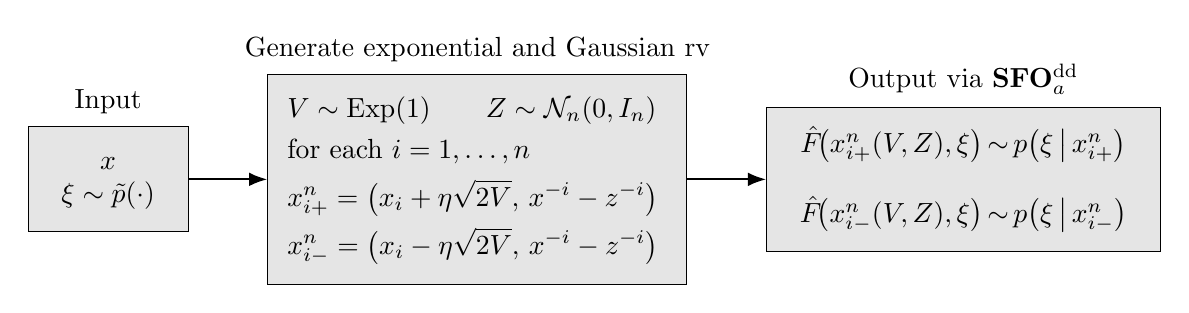
\begin{tikzpicture}[scale = 0.5,
							box/.style={draw, fill=gray!20, rectangle, align=center, inner sep=7pt},
							%bigbox/.style={draw, rectangle, align=center, inner sep=12pt, text width=8.2cm},
							%outbox/.style={draw, rectangle, align=center, inner sep=10pt, text width=8.0cm},
							arrow/.style={-Latex, thick},
							lab/.style={font=\normalsize}
							]
							% --- Input ---
							\node[box] (inp) {$
								\begin{array}{c}
									x\\ %\hline
									\xi \sim \tilde p(\cdot)
								\end{array}
								$};
							\node[lab, above=1pt of inp] {Input};
							% --- Oracle ---
							\node[box, right=1cm of inp] (orc) {%
								$
								\begin{aligned}
									&V \sim \mathrm{Exp}(1)
									\qquad
									Z \sim \mathcal{N}_n(0,I_n)\\
									&\text{for each } i=1,\ldots,n\\
									&x^{n}_{i+}=\bigl(x_i+\eta\sqrt{2V},\,x^{-i}-z^{-i}\bigr)\\
									&x^{n}_{i-}=\bigl(x_i-\eta\sqrt{2V},\,x^{-i}-z^{-i}\bigr)
								\end{aligned}
								$
							};
							\node[lab, above=1pt of orc] {{Generate exponential and Gaussian rv}};
							% --- Output ---
							\node[box, right=1cm of orc] (out) {$
								\begin{array}{c}
									\hat F\!\bigl(x^{n}_{i+}(V,Z),\xi\bigr){\, \sim \,}
									p\!\left(\xi\,\middle|\,x^{n}_{i+}\right)\\%[0.9em]\hline
									\\
									\hat F\!\bigl(x^{n}_{i-}(V,Z),\xi\bigr){\, \sim \,}
									p\!\left(\xi\,\middle|\,x^{n}_{i-}\right)
								\end{array}
								$};
							\node[lab, above=1pt of out] {Output {via {\bf SFO$^{\rm dd}_a$}}};
							% --- Arrows ---
							\draw[arrow] (inp.east) -- (orc.west);
							\draw[arrow] (orc.east) -- (out.west);
						\end{tikzpicture}
						\caption{Oracle schematic for decision dependent stochastic optimization with known struction of $p(\xi \mid x)$}
						\label{fig:oracle-1}
					\end{figure}
					
					
					From \eqref{eq:eta-grad-2}, we get 
					\beq\label{eq:unbiased-dd-1}
					\E_{V,Z, \bxi} [\tilde{g}_{\eta}(x,V,Z, \bxi)] = \nabla f_{\eta}(x).
					\eeq
					We can also derive an analogous second moment bound on the estimator, {which can also be seen to grow linearly with the dimension $n$, akin to the non-DD regime}.
					\begin{proposition}\label{prop:2mombd-DD1}
						Let Assumption~\ref{asm:decdep} holds.  Then for any $x$ and $\eta > 0$,
						\begin{equation*}
							\mathbb{E}_{V,Z,\bxi {\sim \tilde{p}}}\left[\|\tilde{g}_\eta(x,V,Z,\bxi)\|^2\right]\leq {\tfrac{4L_0^2 n}{\pi}}, \mbox{ where } {L_0 \triangleq {\sqrt{2 \lp M^2\hat{L}_f^2 +M M_f^2L_\xi^2 \rp}}},
							%\tfrac{8 \lp M^2\hat{L}_f^2 +M M_f^2L_\xi^2 \rp n}{\pi},
						\end{equation*}
						{ and } $\tilde g_{\eta}$ is defined as in \eqref{estidec1}.
					\end{proposition}
					\begin{proof}
					Observe the non-decision-dependent representation of $f$ in \eqref{eq:dectonondec} and the Lipschitz coefficient $L_0 = {\sqrt{2 \lp M^2\hat{L}_f^2 +M M_f^2L_\xi^2 \rp}}$ of $\tilde{F}$ in Proposition~\ref{lem:F-decdep1-Lip}-(a). Consequently, from Proposition~\ref{prop:secmombd}, we obtain that
					\begin{equation*}
						\mathbb{E}_{V,Z,\bxi {\sim \tilde{p}}}\left[\|\tilde{g}_\eta(x,V,Z,\bxi)\|^2\right]\leq \tfrac{4L_0^2 n}{\pi},
					\end{equation*}
					which proves our result.
					\end{proof}
					\begin{comment}
						For simplicity,  \us{suppose $x^+$ and $x^-$ denote $x^+=x_{i+}^\eta(V,Z)$ and $x^-=x_{i-}^\eta(V,Z)$, respectively.} \us{Suppose the joint density in $V$ and $Z$ is denoted by $c(u)$ where $U = (V,Z)$.}
						%\us{UVS: Mingrui -- please check this below. I changed the notation a bit and cleaned this up. Got rid of $dp(v,z)$ and used $p(u)du$}
						\begin{align}\label{eq:secmodec}
							\mathbb{E}\left[|\tilde{g}^i_\eta(x,V,Z,\bxi)|^2\right]&=\tfrac{1}{2\pi\eta^2}\mathbb{E}_{V,Z,\bxi}\left[\left|\tilde{F}(x^+,\bxi)-\tilde{F}(x^-,\bxi)\right|^2\right]\nonumber\\
							=\tfrac{1}{2\pi\eta^2}\int\int&\left|\frac{\hat{F}(x^+,\xi)p(\xi \mid x^+)}{\tilde{p}(\xi)}-\frac{\hat{F}(x^-,\xi)p(\xi \mid x^-)}{\tilde{p}(\xi)}\right|^2\tilde{p}(\xi)\us{c(u)}d\xi \us{du} \nonumber\\
							&\leq \tfrac{1}{\pi\eta^2}\int \int \left[\left|\hat{F}\left(x^+,\xi\right)-\hat{F}\left(x^-,\xi\right)\right|^2\left|\frac{p(\xi \mid x^+)}{\tilde{p}(\xi)}\right|^2\right.\nonumber\\
							& \quad \quad \left.+{\left|\hat{F}(x^-,\xi)\right|^2} \left|\frac{p(\xi \mid x^+)}{\tilde{p}(\xi)}-\frac{p(\xi \mid x^-)}{\tilde{p}(\xi)}\right|^2\right]\tilde{p}(\xi)\us{c(u)}d\xi \us{du}\nonumber\\
							&\leq \tfrac{1}{\pi\eta^2}\mathbb{E}_{V,Z}\left[L_0^2 \pc{M^2} |x^+-x^-|^2+\int \mr{M_f^2}\left|\frac{p(\xi \mid x^+)}{\tilde{p}(\xi)}-\frac{p(\xi \mid x^-)}{\tilde{p}(\xi)}\right|^2 \tilde{p}(\xi)d\xi\right],
						\end{align}
						\us{where the second inequality follows from the uniform boundedness of $\frac{p(\xi\mid x)}{\tilde{p}(\xi)}$ \pc{by $M$} and $\hat{F}(x,\xi)$ \pc{by $M_f$} for any $x,\xi$}. 
						\us{Consider} the second term in the last line above. 
						\begin{align}\label{eq:seclast}
							\int &\left|\frac{p(\xi \mid x^+)}{\tilde{p}(\xi)}-\frac{p(\xi \mid x^-)}{\tilde{p}(\xi)}\right|^2 \tilde{p}(\xi)d\xi=\int \frac{\left|p(\xi \mid x^+)-p(\xi \mid x^-)\right|^2}{\tilde{p}(\xi)} d\xi\nonumber\\
							&=\int \frac{\left(p(\xi \mid x^+)-p(\xi \mid x^-)\right)_+^2}{p(\xi \mid x^+)}\frac{p(\xi \mid x^+)}{\tilde{p}(\xi)} d\xi+\int \frac{\left(p(\xi \mid x^+)-p(\xi \mid x^-)\right)_-^2}{p(\xi \mid x^-)}\frac{p(\xi \mid x^-)}{\tilde{p}(\xi)} d\xi\nonumber\\
							& \leq Md^2_2\left(p(\xi \mid x^+),p(\xi \mid x^-)\right)+Md^2_2\left(p(\xi \mid x^-),p(\xi \mid x^+)\right).
						\end{align}
						%\us{\bf UVS: We have that $d_2^2$ is defined in terms of distributions, i.e. $d_2^2(\mathbb{Q},\mathbb{P})$; in addition, the above definition is 
							%$$ d_2^2(\mathbb{Q},\mathbb{P}) = \int \frac{(p(\xi) - q(\xi))_+^2}{p(\xi)} d\mu(\xi) $$ 
							%does not match the above.. or maybe I missed something. basically -- extra $\tilde{p}(\xi)$ in denominator.} \pc{-- $p(\xi| x^{+})/\tilde{p}(\xi)$ is bounded by $M$, and the dominating measure $\mu$ is chosen to be Lebesgue. Suggest changing the definition of $d_2$ with $\mu=$Lebesgue since are using densities everywhere. }
						By \cite[Lemma 8.4]{boucheron2013concentration} and Assumption~\ref{asm:decdep} \us{(2)}, we have that
						\begin{equation}\label{eq:KBbound}
							d^2_2\left(p(\xi \mid x^+),p(\xi \mid x^-)\right)+d^2_2\left(p(\xi \mid x^-),p(\xi \mid x^+)\right) \leq D\left(p(\xi \mid x^+),p(\xi \mid x^-)\right) \leq L_0^2|x^+-x^-|^2
						\end{equation}
						Plugging \eqref{eq:seclast} and \eqref{eq:KBbound} into \eqref{eq:secmodec} \us{and noting that $\mathbb{E}[V] = 1$} , we get
						\begin{align}
							\mathbb{E}\left[|\tilde{g}^i_\eta(x,V,Z,\bxi)|^2\right] &\leq  \tfrac{1}{\pi\eta^2}\mathbb{E}_{V,Z}\left[\mr{M^2}L_0^2|x^+-x^-|^2+M\mr{M_f^2}L_0^2|x^+-x^-|^2\right]\nonumber\\
							&\mr{\leq\tfrac{L_0^2M(M+M_f^2)}{\pi\eta^2}\mathbb{E}\left[(2\eta\sqrt{2V})^2\right]=\tfrac{8L_0^2M(M+M_f^2)}{\pi}.}
						\end{align}
					\end{comment}
					%we \us{may derive an analogue} of Lemma~\ref{Lemma:SmoothProperties}. 
					%\begin{lemma}
					%\pc{$f$ defined by \eqref{eq:DDproblem} is Lipschitz with Lipschitz coefficient $\hat{L}_0 = L_0(M + M_f \sqrt{M})$, and consequently satisifies all properties in %Lemma~\ref{Lemma:SmoothProperties}.}
					%\end{lemma}
					%%%%%%%
					\begin{comment}
						\us{\us{\bf UVS: modify to capture decision-dependence. Which constants change?} \pc{perhaps this is not the right place for this lemma--perhaps right after Lemma~\ref{lem:d-2-ineq} or elsewhere if we wish to capture constant for both settings. }
							\begin{lemma}[\mr{Remove this?}]\label{Lemma:SmoothProperties-dec-dep}
								Suppose \pc{either Assum.~\ref{asm:ascvgstochastic} or Assum.~\ref{asm:randomfield} holds and $f, \phi_{\eta},$ and $f_{\eta}$ are defined as in \eqref{eq:DDproblem},  \eqref{eq:phieta}, and \eqref{eq:feta}, respectively. Let $\hat{L_0} = L_0(1+M)$ under Assum.~\ref{asm:decdep} or $\hat{L_0} = L_0 (1+\sqrt{C})$ under Assum.~\ref{asm:randomfield}.} Then the following hold.
								\begin{enumerate}[label=\alph*.]
									\item \label{Lemma:a} %$f_{\eta} \in C^{\infty}$, and 
									The components of $\nabla f_{\eta}$ are given by \eqref{eq:eta-grad-2}\pc{(Assum.~\ref{asm:ascvgstochastic} ) or \eqref{eq:DDGradientfetaD}(Assum.~\ref{asm:randomfield})}.
									\item \label{Lemma:b}$|f_{\eta}(x)-f_{\eta}(y)| \leq \pc{\hat{L_0}} \|x-y\|$ for any $x, y \, \in \, X$.
									\item \label{Lemma:c}$|f_{\eta}(x)-f(x)| \leq \pc{\hat{L_0}}\sqrt{n+1}\eta$ for any $x \, \in \, X$.
									\item \label{Lemma:d} If in addition $f$ is convex, then $f_\eta$ is convex and for any $x \, \in \, X$,
									\begin{equation}\label{eq:Lemmad}
										f(x) \leq f_\eta(x) \leq f(x)+\pc{\hat{L_0}}\sqrt{n+1}\eta.
									\end{equation}
									\item \label{Lemma:e} $\|f_\eta(x)-f_{\eta^{\prime}}(x)\| \leq \pc{\hat{L_0}}\sqrt{n+1}|\eta-\eta^{\prime}|$.
									\item \label{Lemma:f} $\|\nabla f_{\eta}(x) - \nabla f_{\eta}(y)\| \leq \frac{2\pc{\hat{L_0}}\sqrt{n}}{\eta \sqrt{2 \pi}}\|x-y\|$ for any $x, y \, \in \, X$.
									\item \label{Lemma:g} If $f$ is differentiable and $L_1$-smooth, then $\|\nabla f_{\eta}(x) - \nabla f(x)\| \leq L_1\eta \sqrt{n}$ for any $x \, \in \, X$.
								\end{enumerate}
							\end{lemma}
							\pc{
								\begin{proof}
								To be completed: but just show $f(x) = \E_{\bxi \sim \mathcal{D}(x)} [\hat{F} (x, \bxi)]$ is $\hat{L}_0$-Lipschitz. 
								\end{proof}
							}
						}
					\end{comment}
					%%%%%%%%%
					%\pc{CAUTION!!! Change $L_0$ to $\hat{L_0}$ wherever $\hat{F}$ is assumed to be $\hat{L_0}$-Lipschitz}
					
					%%%%%%
					\begin{comment}
						\begin{remark}[\mr{(Remove this remark.)}]
							One \us{may} also be curious about whether there is relation between the stationary point and the ``equilibrium'' point of the problem~\ref{eq:DDproblem} \us{as defined in XX.}. By definition~\ref{def:eq}, we have for an equilibrium point $\bar{x}$, \us{the following condition holds.}
							\begin{equation*}
								\int \nabla_x \hat{F}(x,\xi)p(\xi \mid \bar{x}) dx \Big|_{x=\bar{x}}=0.
							\end{equation*} 
							However, \us{at an unconstrained stationary point},  we have \us{that the following holds.}
							\begin{equation}\label{eq:stpgrad}
								\int \us{(}\nabla_x \hat{F}(x,\xi)p(\xi \mid x) +\hat{F}(x,\xi)\nabla_x p(\xi \mid x) \us{)}dx \Big|_{x=x^*}=0.
							\end{equation} 
							By assuming that for any $p(\xi \mid x)\leq M$ \us{for any $x, \xi$}), we proceed to \us{derive a bound on the first term in \eqref{eq:stpgrad}. We first observe that} 
							\begin{align*}
								&\int\left|p(\xi \mid x_1)-p(\xi \mid  x_2)\right|^2d\xi \\
								&=\int \frac{\left(p(\xi \mid x_1)-p(\xi \mid x_2)\right)_+^2}{p(\xi \mid x_1)}p(\xi \mid x_1)d\xi+\int \frac{\left(p(\xi \mid x_1)-p(\xi \mid x_2)\right)_-^2}{p(\xi \mid x_2)}p(\xi \mid x_2)d\xi\\
								&\leq Md^2_2\left(p(\xi \mid x_1),p(\xi \mid x_2)\right)+Md^2_2\left(p(\xi \mid x_2),p(\xi \mid x_1)\right)\\
								&\leq MD\left(p(\xi \mid x_1),p(\xi \mid x_2)\right) \leq L_0^2|x_1-x_2|^2.
							\end{align*}
							We have \us{\bf UVS: Please justify interchange of limit and integral and the inequality.} \pc{(If DCT is used to justify interchange, need Lipschitz $|p(\xi|x) - p(\xi|y)| \leq g(\xi){\|x-y\|}$, and $g(\xi)$ integrable. but then above calculations are perhaps not required)}
							\begin{equation*}
								\int \left|\nabla_x p(\xi \mid x)\right|^2d\xi \leq \lim_{|x_1-x_2| \rightarrow 0} \int\frac{\left|p(\xi \mid x_1)-p(\xi \mid  x_2)\right|^2}{|x_1-x_2|^2}d\xi \leq ML_0^2.
							\end{equation*}
							Then by Cauchy-Schwarz, the second term of \eqref{eq:stpgrad}
							\begin{equation*}
								\left|\int \hat{F}(x,\xi)\nabla_x p(\xi \mid x) dx\right|^2\leq \left(\int \hat{F}^2(x,\xi)d\xi\right)^{1/2}\left( \int\left|\nabla_x p(\xi \mid x)\right|^2d\xi \right)^{1/2} \leq ML_0^2M_f.
							\end{equation*}
							\us{\bf This ends abruptly..we have a bound on the second term. What can we conclude?} \pc{the ultimate goal to get a bound on $|\bar{x} - x^{\ast}|$, but this gives a bound at $x = x^{\ast}$ of the first quantity $\int \nabla_x \hat{F}(x,\xi)p(\xi \mid {x}^{\ast}) dx \Big|_{x={x}^{\ast}}$. Maybe this could be completed Mingrui.}
						\end{remark}
					\end{comment}
					%%%%%%%%%%%
					
					\subsection{Unknown structure of $p(\xi \mid x)$.}\label{sub:p_unknown} 
					In this subsection, we consider the more common setting where the functional form of $p(\bullet \mid x)$ is unavailable. Yet, we proceed to show that similar guarantees can be obtained under some assumptions.  We use the same notation $x_{i+}^\eta{(V,Z)}$ and $x_{i-}^\eta{(V,Z)}$, as defined in \eqref{eq:x_i+-}. Note that in this setting, we do not introduce a density $\tilde{p}(\bullet)$.
					%\begin{align*}
					%	x_{i+}^\eta(v,z)=\left(x_i+\eta\sqrt{2v},x^{-i}-z^{-i}\right) \mbox{ and }
					%	x_{i-}^\eta(v,z)=\left(x_i-\eta\sqrt{2v},x^{-i}-z^{-i}\right),
					%\end{align*}
					%respectively. 
					Our first result derives the gradient of $f_{\eta}$ when $p(\xi\mid x)$ is unavailable. 
					Contrary to our exposition in the prequel, we are going to assume existence of a random field ${\bxi} = \{\bxi_{x}, x \in \R^n\}$ which exhibit the marginals $\cd(x)$ or $p(\xi \mid x)$ (when density exists) for every $x \in \R^n$, in addition to a correlation structure we define below. To talk about expectations of functionals with respect to this random field, we will also employ the following notation for expectation of any function $u(x,y,\bxi_x,\bxi_y)$ with respect to $\bxi$, defined as %\mr{\bf MR: Should this be integral w.r.t the joint density?}     
					\begin{equation}\label{eq:Expxi12}
						\mathbb{E}_{\bxi_x, \bxi_y} \left[ \, u(x,y,\bxi_x,\bxi_y)\, \right] \, \triangleq \, \int_{\Xi(y)} \ \int_{\Xi(x)} \ u(x,y, \xi_1, \xi_2) p_{\bxi_x, \bxi_y}(\xi_1, \xi_2) d\xi_1 d\xi_2,
					\end{equation}
					where $p_{\bxi_x, \bxi_y}$ is the joint density of $(\bxi_x,\bxi_y)$, with marginals $\bxi_x \sim \mathcal{D}(x),\bxi_y \sim \mathcal{D}(y)$.
					Unless mentioned otherwise, in this subsection, the expectation operator is as defined above. We now outline some assumptions on $\bxi$ and $\hat{F}$, {based on which we may conclude}  the Lipschitzian property of $f$. %specifically imposing a suitable Lipschiztian requirement on $\hat{F}$.  %We first assume a relation on the correlation structure of the random field $\{\bxi_{x}; x \in \R^n\}$. 
					\begin{assumption}\label{asm:randomfield}
						$\hat{F}(\bullet,\xi_\bullet)$ is $L_0$-Lipschitz continuous in the $L^2(\bxi_\bullet)$ metric, i.e., there exists an $L_0$ such that the following holds for any $x, y \in \R^n$.
						$$
						{\lnn \hat{F}(x, \bxi_x) - \hat{F}(y, \bxi_y) \rnn}_{L^2(\bxi_\bullet)} \, \leq \, L_0 \|x-y\|.
						$$  
					\end{assumption}
					
					In this section, we assume existence of a stochastic first-order oracle {\bf SFO$^{\rm dd}_u$} corresponding to a decision-dependent regime with an unknown density $p(\xi\mid x)$.\\
					
					\begin{definition} [{\bf SFO$^{\rm dd}_u$}] \label{sfo-ddu} There exists a stochastic first-order oracle that given {a collection $x\in {\laa}$, produces $\{ \hat{F}(x,\xi_x); x \in {\laa} \}$},  where {$\{\xi_x ; x \in {\laa} \}$} is generated from an identical but independent random field that satisfies the Assumption~\ref{asm:randomfield} with the marginal distribution $\bxi_x \sim \mathcal{D}(x)$.  %with unknown density density $p(\xi\mid x)$.  
					\end{definition}
					
					%\us{[\bf UVS: Seek clarification.}\pc{- definition modified slightly - please check]}}
				%\mr{\noindent \emph{Oracle.} In this subsection, the oracle does not have access to the density $p(\bullet\mid x)$. When an input $x$ is provided to the oracle, it provides an output $\xi_x$ or $\hat{F}(x, \xi_x)$. However, it is important to note that at each iteration, $\xi_x$ is generated from an identical but independent random field that satisfies the Assumption~\ref{asm:randomfield} with the marginal distributions $\bxi_x \sim \mathcal{D}(x)$.}
				%\us{We observe that this assumption is indeed satisfied under a suitable correlation requirement on $\bxi_x$ and $\bxi_y$, as we subsequently observe.}
				
				
				\begin{figure}[h]
					\centering
					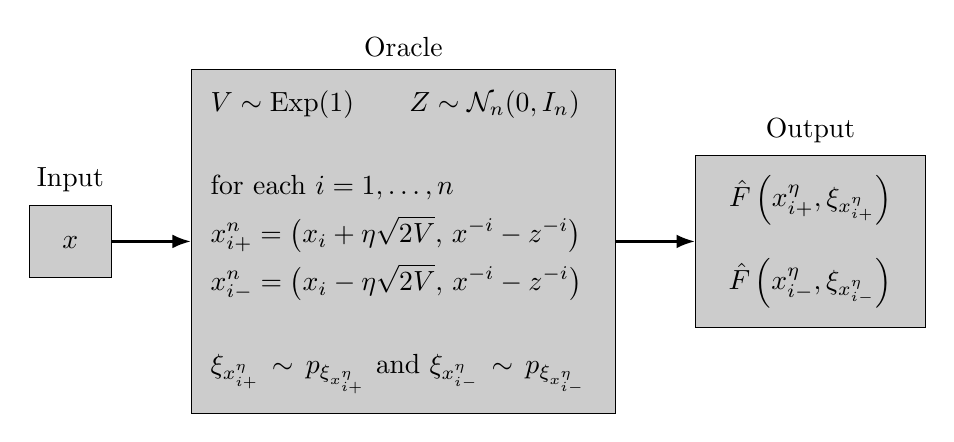
\begin{tikzpicture}[scale = 0.5,
						box/.style={draw, rectangle, fill=gray!40, align=center, inner sep=7pt},
						%bigbox/.style={draw, rectangle, align=center, inner sep=12pt, text width=8.2cm},
						%outbox/.style={draw, rectangle, align=center, inner sep=10pt, text width=8.0cm},
						arrow/.style={-Latex, thick},
						lab/.style={font=\normalsize}
						]
						% --- Input ---
						\node[box] (inp) {$
							\begin{array}{c}
								x%\\ \hline
								%\xi \sim \tilde p(\cdot)
							\end{array}
							$};
						\node[lab, above=1pt of inp] {Input};
						% --- Oracle ---
						\node[box, right=1cm of inp] (orc) {%
							$
							\begin{aligned}
								&V \sim \mathrm{Exp}(1)
								\qquad
								Z \sim \mathcal{N}_n(0,I_n)\\
								&\\
								&\text{for each } i=1,\ldots,n\\
								&x^{n}_{i+}=\bigl(x_i+\eta\sqrt{2V},\,x^{-i}-z^{-i}\bigr)\\
								&x^{n}_{i-}=\bigl(x_i-\eta\sqrt{2V},\,x^{-i}-z^{-i}\bigr)\\
								&\\
								&{\xi_{x_{i+}^\eta} \, \sim \,  p_{\xi_{x_{i+}^\eta}}} \mbox{ and } {\xi_{x_{i-}^\eta}  \, \sim \,  p_{\xi_{x_{i-}^\eta}}}
							\end{aligned}
							$
						};
						\node[lab, above=1pt of orc] {Oracle};
						% --- Output ---
						\node[box, right=1cm of orc] (out) {$
							\begin{array}{c}
								\hat{F} \left(x_{i+}^{\eta}, \xi_{x_{i+}^{\eta}} \right)\\%[0.9em]\hline
								\\
								\hat{F} \left(x_{i-}^{\eta}, \xi_{x_{i-}^{\eta}} \right)
							\end{array}
							$};
						\node[lab, above=1pt of out] {Output};
						% --- Arrows ---
						\draw[arrow] (inp.east) -- (orc.west);
						\draw[arrow] (orc.east) -- (out.west);
					\end{tikzpicture}
					\caption{Oracle schematic for decision dependent stochastic optimization with unknown struction of $p(\xi \mid x)$}
					\label{fig:oracle-2}
				\end{figure}
				
				
				\begin{remark}\label{ass:f-hat-Lip-DD2}
					Naturally, one might inquire if the prior Assumption ~\ref{asm:randomfield} is vacuous. We observe that under the following correlation and Lipschitzian requirements, this assumption indeed holds. 
					%For better understanding, we here provide a more explicit assumption in the following.
					\begin{enumerate}
						\item\label{ass:DD2-xi} For any $x,y\in \R^n$, there exists a constant $c_{\xi}$ such that $\mathbb{E}[\|\bxi_x-\bxi_y\|^2] \, \leq \, c_{\xi} \|x-y\|^2$ for $\bxi_x \sim \mathcal{D}(x),\bxi_y \sim \mathcal{D}(y)$, i.e.,   $\bxi$ is $L_2$-Lipschitz. 
						\item $\hat{F}(x,\xi)$ is $L_\xi$-Lipschitz in $x$ and $\xi$.
					\end{enumerate}
					It is readily checked that if the above two requirements are satisfied then Assumption~\ref{asm:randomfield} will be satisfied with $L_0=L_\xi\sqrt{2+2c_\xi}$. 
					 
				\end{remark}
				\medskip
				Examples of $L_2$-Lipschitz random fields are aplenty. We provide two simple Gaussian examples. For further details please refer to \cite{gaussian-processes-ml}.\\
				\begin{enumerate}[wide, labelindent = 0pt, label = (\roman*)]
					\item {Let $\{\psi_k\}_{k=1}^n$ be deterministic continuous functions and $\{Z_k\}_{k=1}^n$ be independent standard normals}. {If $\{a_k\}_{k=1}^n$ denotes a set of scalars, then }
					$$\bxi_x = \sum_{k=1}^n a_k Z_k \psi_k(x)$$
					is a centered Gaussian random field satisfying the $L_2$-Lipschitz property.
					\item Let $W$ be Gaussian white noise on $\R^d$. Then for a kernel $\phi \in L^2$ with bounded gradient, the Gaussian convolutional random field
					$$\bxi_x = \int \phi(x-u) W(du)$$
					satisfies the $L_2$-Lipschitz property.
				\end{enumerate}
				
				As one may notice, $\bxi_x,\bxi_y$ in Assumption~\ref{asm:randomfield} or Remark~\ref{ass:f-hat-Lip-DD2} cannot be independent. Assumption~\ref{asm:randomfield}  suffices to guarantee the Lipschitz continuity of the function $f$. 
				%\us{\bf We need to be precise about what the expectation is wrt? $\mathbb{E}_{V,Z,\bxi_{+},\bxi_{-}}$?}
				%\us{\bf Some notational suggestions here. Why not use $\bxi_{x_{i+}^\eta}$ and $\bxi_{x_{i-}^\eta}$ rather than $\bxi_{1},\bxi_{2}$? This helps clarify the Lipschitzian structure below.} \pc{Yes this change been pending too long.}
				
				\begin{lemma}\label{lem:f-decdep2-Lip}
					Suppose Assumption~\ref{asm:randomfield} holds. Then $f$, defined in \eqref{eq:DDproblem}, is $L_0$-Lipschitz continuous. %all previous results we derived for non-decision-dependent problem will hold for decision-dependent problem.
				\end{lemma}
				\begin{proof} 
				Recall from \eqref{eq:DDproblem} that $f(x)=\int_{\Xi(x)} \hat{F}(x, \xi)p(\xi \mid  x) d\xi$. Consequently, by Jensen's inequality, for any $x, y$, we have  
				\begin{align*}
					|\, f(x)-&f(y)\, |\, = \, \left|\, \mathbb{E}_{\bxi_x, \bxi_y}\left[\, \hat{F}(x,\bxi_x)-\hat{F}(y,\bxi_y)\, \right]\, \right|\\
					&\, \leq \, \sqrt{\E_{\bxi_x,\bxi_y}\left[\, \left| \,\hat{F}(x,\bxi_x)-\hat{F}(y,\bxi_y)\, \right|^2 \, \right]}\, =\, {\lnn \hat{F}(x, \bxi_x) - \hat{F}(y, \bxi_y) \rnn}_{L^2(\bxi_\bullet)} \leq L_0 \|x-y\|.
				\end{align*}
				\end{proof}
				This result allows us to claim that Proposition ~\ref{prop:gradfeta} and Lemma~\ref{Lemma:SmoothProperties} hold true with Lipschitz constant $L_0$. 
				\begin{proposition}\label{prop:DDgradfeta}
					Suppose Assumption~\ref{asm:randomfield} holds. Let $\phi$ and $\phi_\eta$ be as in \eqref{eq:phiu} and \eqref{eq:phietau}. %\pc{\sout{Let $f \in L^1(\mathbb{R}^n,\mathbb{R})$ and $f_\eta$ as introduced in \eqref{eq:feta}}}. 
					Then for $1 \leq i \leq n$, the $i$-th partial derivative of $f_\eta$ is given by 
					\begin{equation}\label{eq:DDGradientfetaD}
						\tfrac{\partial_i f_{\eta}(x)}{\partial x_i} \,  = \, \tfrac{1}{\eta\sqrt{2\pi}}\mathbb{E}_{{V,Z,\bxi_{x_{i+}^\eta},\bxi_{x_{i-}^\eta}}}\left[\hat{F}\left(x_{i+}^\eta(V,Z), \bxi_{x_{i+}^\eta}\right)-\hat{F}\left(x_{i-}^\eta(V,Z), \bxi_{x_{i-}^\eta}\right)\right],
					\end{equation}
					where the expectation taken over $\bxi_{x_{i+}^\eta},\bxi_{x_{i-}^\eta}$ is in the sense of \eqref{eq:Expxi12} with marginals $ \mathcal{D}(x_{i+}^\eta(V,Z))$ and $\mathcal{D}(x_{i-}^\eta(V,Z))$, respectively. Additionally, $V \sim \mathcal{E}xp(1)$ and $Z\sim \mathcal{N}_n(0,\eta^2 I)$.
				\end{proposition}
				\begin{proof}
				By invoking Lemma~\ref{lem:f-decdep2-Lip}, we have that $f$ is $L_0$-Lipschitz continuous. Therefore. we may apply Proposition~\ref{prop:gradfeta}. By \eqref{eq:GradientfetaD} and using the representation of $f$ in \eqref{eq:DDproblem} it is immediate that
				\begin{align*}
					\tfrac{\partial_i f_{\eta}(x)}{\partial x_i}&=
					\, \tfrac{1}{\eta \sqrt{2\pi}}\mathbb{E}_{V,Z}\left[f\left(x_{i+}^{\eta}(V,Z)\right)-f\left(x_{i-}^{\eta}(V,Z) \right)\right] \\
					%&\tfrac{1}{\eta\sqrt{2\pi}}\left[\int_{0}^{+\infty} f\left(x_i+\eta\sqrt{2v},x^{-i}-z^{-i}\right)h(v) dv  \right.\\
					%&\quad \quad\left.-\int_{0}^{+\infty} f\left(x_i-\eta\sqrt{2v},x^{-i}-z^{-i}\right)h(v) dv \right]\\
					%&=\tfrac{1}{\eta\sqrt{2\pi}}\left[\int_{0}^{+\infty} \int_{\Xi(x)} \hat{F}\left(x_{i+}^\eta(v,z), \xi\right)p\left(\xi \mid x_{i+}^\eta(v,z)\right) d\xi \, h(v) dv \right.\\
					%&\quad \left. \quad -\int_{0}^{+\infty} \int_{\Xi(x)}  \hat{F}\left(x_{i-}^\eta(v,z), \xi\right)p\left(\xi \mid x_{i-}^\eta(v,z)\right) d\xi \, h(v) dv \right]\\
					&=\tfrac{1}{\eta\sqrt{2\pi}}\mathbb{E}_{V,Z,\bxi_{x_{i+}^\eta},\bxi_{x_{i-}^\eta}}\left[\hat{F}\left(x_{i+}^\eta(V,Z), \bxi_{x_{i+}^\eta}\right)-\hat{F}\left(x_{i-}^\eta(V,Z), \bxi_{x_{i-}^\eta}\right)\right].
				\end{align*}	%where we used the representationin \eqref{eq:DDproblem}.
				\end{proof}
				
				Denote $\bxi_{x_+^\eta}=(\bxi_{x_{i+}^\eta})_{1\leq i\leq n}$ and $\bxi_{x_-^\eta}=(\bxi_{x_{i-}^\eta})_{1\leq i\leq n}$. Let us consider a new gradient estimator $\tilde{g}_{\eta}$, where the $i$-th component $\tilde{g}_{\eta}^i$ is defined as 
				\begin{equation*}
					\tilde g_{\eta}^i \left(x,v,z,\xi_1,\xi_2\right) \, = \,\tfrac{1}{\eta\sqrt{2\pi}}\left(\hat{F}\left(x_{i+}^\eta(v,z), \xi_1\right)-\hat{F}\left(x_{i-}^\eta(v,z), \xi_2\right)\right)
				\end{equation*}
				and $\xi_1$ and $\xi_2$ denote realizations of $\bxi_{x_+^\eta}$ and $\bxi_{x_-^\eta}$, respectively. As a result of Proposition~\ref{prop:DDgradfeta}, $\tilde{g}_{\eta}$ is an unbiased estimate of $\nabla f_{\eta}$, as qualified in: 
				\beq\label{eq:unbiasedd-dd-2}
				\E_{V,Z,\bxi_{x_+^\eta},\bxi_{x_-^\eta}}  \left[\, \tilde{g}_{\eta}(x,V,Z,\bxi_{x_{+}}, \bxi_{x_{-}}) \, \right]  \, = \, \nabla f_{\eta}(x).
				\eeq
				This then allows for deriving an analogous second moment bound on the estimator {with a similar dependence (linear) on $n$ as in the prior two estimators.}
				\begin{proposition}\label{prop:DDsecmombd}
					Suppose Assumption~\ref{asm:randomfield} holds. Then for any $x\in \R^n$ and $\eta > 0$,
					\begin{equation}
						\mathbb{E}\left[\, \|\tilde{g}_\eta(x,V,Z,\bxi_{x_{+}^{\eta}},\bxi_{x_{-}^{\eta}})\|^2\, \right] \, \leq \, \tfrac{4L_0^2n}{\pi}.
					\end{equation}
				\end{proposition}
				\begin{proof}
				Consider an $L_\xi$-Lipschitz continuous $\hat{F}$. Then 
				%\us{\bf UVS: May be worth qualifying what the expectation is wrt as seen below?}\pc{I think we have been using the convention of specifying variables when expectation is {\bf not} taken over all random variables-- but we should check if this is followed everywhere.}
				\begin{align*}
					& \quad \mathbb{E}_{V,Z,\bxi_{x_{i+}^\eta},\bxi_{x_{i-}^\eta}}\left[\left|\, \tilde g_{\eta}^i\left(x,V,Z,\bxi_{x_{i+}^\eta},\bxi_{x_{i-}^\eta}\right)\right|^2\right] \\
					& = \tfrac{1}{\eta^2 2\pi}\mathbb{E}_{V,Z,\bxi_{x_{i+}^\eta},\bxi_{x_{i-}^\eta}}\left[\left|\hat{F}\left(x_{i+}^\eta(V,Z), \bxi_{x_{i+}^\eta}\right)-\hat{F}\left(x_{i-}^\eta(V,Z), \bxi_{x_{i-}^\eta}\right)\right|^2\right]\\
					&= \tfrac{1}{\eta^2 2\pi} \mathbb{E}_{V,Z} \left\|\hat{F}\left(x_{i+}^\eta(V,Z), \bxi_{x_{i+}^\eta}\right)-\hat{F}\left(x_{i-}^\eta(V,Z), \bxi_{x_{i-}^\eta}\right)\right\|_{L^2(\bxi_\bullet)}^2.
				\end{align*}
				Then by Assumption~\ref{asm:randomfield} we have
				$$
				\mathbb{E}_{V,Z,\bxi_{x_{i+}^\eta},\bxi_{x_{i-}^\eta}}\left[\left|\, \tilde g_{\eta}^i\left(x,V,Z,\bxi_{x_{i+}^\eta},\bxi_{x_{i-}^\eta}\right)\right|^2\right]
				\leq \tfrac{1}{\eta^2 2\pi}L_0^2 \mathbb{E}_{V,Z} \left[\, \left|x_{i+}^\eta(V,Z)-x_{i-}^\eta(V,Z)\right|^2 \, \right] =\frac{4L_0^2}{\pi}.
				$$
				%\end{align*}
				%\us{UVS: We use Jensen's above -- qualify this step and clarify it's usage since our expectation is decision-dependent.}
				Then the result follows by noting that $\mathbb{E}[\|\tilde{g}_{\eta}(x,V,Z,\bxi_{x_{i+}^\eta},\bxi_{x_{i-}^\eta})\|^2]=\sum_{i=1}^n \mathbb{E}[|\tilde{g}_{\eta}^i(x,V,Z,\bxi_{x_{i+}^\eta},\bxi_{x_{i-}^\eta})|^2]$.
				
				\end{proof}
				
				\begin{remark}
					The need for Assumption~\ref{asm:randomfield}.\ref{ass:DD2-xi} is clear from the proof of Proposition~\ref{prop:DDsecmombd}. Simply speaking, one requires that $\hat{F}(x_{+}^{\eta}(V,Z),\bxi_{x_{+}})$ and $\hat{F}(x_{-}^{\eta}(V,Z),\bxi_{x_{-}})$ be correlated in order to bound the second moment of $\tilde g_{\eta}$. One way to achieve that is by imposing Assumption~\ref{asm:randomfield}.\ref{ass:DD2-xi} on the random field $\{\bxi_x; x \in \R^n\}$. Note that in Section~\ref{sub:p_known}, such dependence is also needed but created artificially between $\tilde F(x_{+}^{\eta}(V,Z), \bxi)$ and $\tilde F(x_{-}^{\eta}(V,Z), \bxi)$ as evident in the definition of $\tilde g_{\eta}$ in \eqref{estidec1}. 
				\end{remark}
				
				%\us{UVS: We will need to provide some instances where Assumption 3.2 does hold. I think we discussed settings with the Gaussian distribution where the mean is affected by $x$. }
				\subsection{Optima, stationary points, and performatively stable points}
				Early work in decision-dependent stochastic optimization problems, as outlined in ~\cite{drusvyatskiy2023stochastic, perdomo2020performative}, focused on an examination of a  ``performative stable point'' or an ``equilibrium'' point.  In general, such a point is distinct from either an optimal solution or a stationary point.  We recap the three distinct  definitions.
				
				\medskip
				
				\begin{definition}\label{def:eq}
					Consider the decision-dependent problem \eqref{eq:DDproblem}. 
					
					\noindent (i) $x^{\rm opt}$ is an optimal solution of \eqref{eq:DDproblem}, if 
					\begin{align}
						f(x^{\rm opt}) \, \le \, f(x) = \mathbb{E}_{\bxi \sim {\mathcal{D}}(x)} \left[ F(x,\bxi) \right], \quad \forall x \, \in \, X.
					\end{align}
					\noindent (ii) If $f$ is C$^1$ on an open neighborhood containing $X$, then $x^{\rm stat}$ is a stationary point of \eqref{eq:DDproblem} if 
					\begin{align}
						\nabla_x f(x)^\top (y - x) \, \ge \, 0, \quad \forall y \, \in \, X.
					\end{align}
					\noindent (iii)  $x^{\rm ps} \in X$ is called a performatively stable point  of  \eqref{eq:DDproblem} if
					\begin{equation}
						x^{\rm ps} \, \in \, {\displaystyle \text{arg}\hspace{-0.01in}\min_{x \, \in \, X}} \, \mathbb{E}_{\bxi \sim \mathcal{D}({x^{\rm ps}})} \left[\hat{F}(x, \bxi)\right]. 
					\end{equation} 
				\end{definition}
				{It may be noted that a performatively stable point, denoted by}  $x^{\rm ps}$, satisfies a fixed-point property by definition. While the relationship between optima and stationary points is well studied in the optimization literature, we point out two other relationships, one of which is less obvious, showing that if the distribution function satisfies a suitably defined ${\beta}$-sensitivity with respect to $x$, then under suitable strong convexity and Lipschitzian requirements, then $\|x^{\rm opt}-x^{\rm ps}\| = \mathcal{O}({\beta})$. {However, such a parameter $\beta$ is idiosyncratic to the problem setting, suggesting that $x^{\rm opt}$ and $x^{\rm ps}$ need not be close to zero.  } 
				
				\begin{lemma} Consider the decision-dependent problem \eqref{prob-dd}. Then the following hold.
					
					\noindent (a) $f(x^{\rm opt}) \, \le \, f(x^{\rm ps}).$
					
					\noindent (b) Suppose $F(x,\xi)$ is $\gamma$-strongly convex in $x$ for any $\xi$ and $L_{\xi}$-Lipschitz in $\xi$ for any $x$. Further, suppose ${\mathcal{D}}(\cdot)$ is ${\beta}$-sensitive, i.e., if $W_1({\mathcal{D}}(x),{\mathcal{D}}(x^\prime)) \le {\beta} \| x-x^\prime\|$ for any $x,x^{\prime} \in X$. Then for any $x^{\rm opt}$ and any $x^{\rm ps}$, 
					$$\| x^{\rm opt}-x^{\rm ps} \| \, \le \, \frac{2L_{\xi} {\beta}}{\gamma}.$$  
				\end{lemma}
				\begin{proof} (i) Omitted; (ii) See \cite[Theorem 4.3]{perdomo2020performative}.
				\end{proof}
				
				\medskip
				
				More generally, absent strong assumptions on the distribution and the stringent convexity requirements, a performatively stable solution $x^{\rm ps}$ may be significantly poorer than the optimal solution $x^{\rm opt}$ and may 
				%even display any desirable stationarity property.    Even if the function $\hat{F}(x, \xi)$ is strongly convex in $x$ for all $\xi \in \Xi$, its expectation $\mathbb{E}_{\bxi \sim \mathcal{D}(x)} [\hat{F}(x, \bxi)]=\int_{\Xi(x)} \hat{F}(x, \xi)p(\xi \mid  x) d\xi$ may still be nonconvex in $x$. In fact, it appears that an equilibrium point, as defined next, may 
				have no corresponding stationarity guarantee. Consequently, the definition of an optimal point requires careful consideration.
				%\medskip
				Observe that
				\begin{align}
					f_\eta(x) & =\int f(y) \phi_\eta(x-y) \, d y  =\int \mathbb{E}\left[\hat{F}\left(y, \bxi_y\right)\right] \phi_\eta(x-y) \, d y \nonumber\\
					& \stackrel{\text{Fubini}}{=}\underbrace{\mathbb{E}\left[\int \hat{F}\left(y, \bxi_y\right) \phi_\eta(x-y) \, d y\right]}_{\, =\mathbb{E}_{\bxi {\sim {\mathcal{D}}(y)}} \left[\bar{F}_\eta(x, \bxi)\right]} \label{eq:DDeqf1}\\
					& =\mathbb{E}\left[\int \hat{F}\left(x-y, \bxi_{x-y}\right) \phi_\eta(y) \, d y\right] \nonumber
					=\mathbb{E}_{\bxi}\left[\mathbb{E}_{Z_\eta}\left[\hat{F}\left(x-Z_\eta, \bxi_{x-Z_\eta}\right)\right]\right]\notag \\
					& =\mathbb{E}_{{\bxi \sim {\mathcal{D}}(x-Z_{\eta}), Z_{\eta}}}\left[\hat{F}\left(x-Z_\eta, \bxi\right)\right], \label{eq:DDeqf2}
				\end{align}
				where $Z_\eta$ denotes a random variable with probability density function $\phi_\eta$. Observe that this representation reveals that the decision dependence is no longer local (i.e. at $x$) but is instead  spread over the feasible region through $x-Z_{\eta}$.
				%Equations \eqref{eq:DDeqf1} and \eqref{eq:DDeqf2} indicate that the equilibrium point, as characterized in Definition~\ref{def:eq}, is not a suitable solution concept for the smoothed problem. This is because the decision dependence is smoothed or convoluted over the feasible region $X$, resulting in a non-local dependence on the random field $\bxi$. 
				This necessitates a new definition of equilibrium for the smoothed problem, provided next.  \\
				
				\begin{definition}\label{def:etasmeq}
					$\bar{x}_\eta$ is a $\eta$-smoothed {performatively stable point} of the decision-dependent problem \eqref{eq:DDproblem} if
					\begin{equation*}
						\bar{x}_\eta  \, {\in} \, \arg\min_{x\in X}\E_{\bxi}\left[\E_{Z_{\eta}}\left[\hat{F}\left(x-Z_\eta,\bxi_{\bar{x}_\eta-Z_\eta}\right)\right]\right]. 
					\end{equation*} 
					
				\end{definition}
				
				\medskip
				
				A natural question is whether the $\eta$-smoothed {perfomatively stable point} is an approximate {performatively stable point} for the original problem. We show below that this is indeed the case with the following enhanced version of Assumption~\ref{asm:randomfield}.
				%This is indeed provable as captured by the next result. 
				%\mr{\bf MR: I plan to delete the following Proposition. I was not careful before... I realize that actually $ f_\eta(x)\neq \mathbb{E}_{\bxi \sim \mathcal{D}(x)} [\hat{F}_\eta(x, \bxi)]$. And it doesn't make sense to talk about the equilibrium of the smoothed problem because the smoothed problem $\min f_\eta(x)$ is not of expectation form anymore.}
				\begin{proposition}
					%\us{UVS: We need to claim that $f$ as defined in the DD-case is indeed $\bar{L}$-Lipschitz since we use this below. Maybe specify the assumptions required for that.}
					Suppose $\varepsilon > 0$ and there exists an $\bar{L}$ such that the following holds for any $x, y \in \R^n$.
					\begin{equation}\label{eq:asmenhance}
						{\lnn \hat{F}(x_1, \bxi_{x_2}) - \hat{F}(y_1, \bxi_{y_2}) \rnn}_{L^2(\bxi_\bullet)} \, \leq \, \frac{\bar{L}}{2} \left(\|x_1-y_1\|+\|x_2-y_2\|\right).
					\end{equation} Let $\bar{x}_\eta$ be an $\eta$-smoothed {performatively stable point} as in Definition~\ref{def:etasmeq} with $\eta \leq \tfrac{\varepsilon}{2\bar{L}\sqrt{n+1}}$. Then $\bar{x}_\eta$ is an $\varepsilon$-{performatively stable point} of the original problem $\min f(x)= \mathbb{E}_{\bxi \sim \mathcal{D}(x)} [\hat{F}(x, \bxi)]$.
				\end{proposition}
				\begin{proof}
				Observe that by Lemma~\ref{Lemma:SmoothProperties} \eqref{Lemma:c} for any $x \in X$ and by definition of the smoothing, we have
				\begin{align}\label{eq:fxbareta}
					\notag	f(\bar{x}_\eta) & = \mathbb{E}_{\bxi} \left[\hat{F}(\bar{x}_\eta, \bxi_{\bar{x}_\eta})\right] \,\leq \, f_\eta(\bar{x}_\eta)+\bar{L}\eta\sqrt{n+1}\\
					& =\E_{\bxi}\left[\E_{Z_\eta}\left[\hat{F}\left(\bar{x}_\eta-Z_\eta, \bxi_{\bar{x}_\eta-Z_\eta}\right)\right] \right]+\bar{L}\eta \sqrt{n+1}.
				\end{align}
				By definition of $\bar x_{\eta}$ and Fubini's theorem, the following holds for any $x \in X$,	
				\begin{equation}\label{eq:xbareta}
					\E_{\bxi}\left[\E_{Z_\eta}\left[\hat{F}\left(\bar{x}_\eta-Z_\eta, \bxi_{\bar{x}_\eta-Z_\eta}\right)\right] \right]\leq \E_{Z_\eta}\left[\E_{\bxi}\left[\hat{F}\left(x-Z_\eta, \bxi_{\bar{x}_\eta-Z_\eta}\right)\right] \right].
				\end{equation}	
				Furthermore, by Jensen's inequality we have for any $x \in X$%through a second application of Lemma~\ref{Lemma:SmoothProperties} leads to the following claim for any $x \in X$.
				\begin{align*}
					& \left|\E_{Z_\eta}\left[\E_{\bxi}\left[\hat{F}\left(x-Z_\eta, \bxi_{\bar{x}_\eta-Z_\eta}\right)\right]\right]-\E_{\bxi}\left[\hat{F}(x,\bxi_{\bar{x}_\eta})\right]\right|  \\
					&~~~~ \leq \E_{Z_\eta}\left[\, \left\|\hat{F}\left(x-Z_\eta, \bxi_{\bar{x}_\eta-Z_\eta}\right)-\hat{F}(x,\bxi_{\bar{x}_\eta})\right\|_{L^2(\bxi_{\bullet})} \, \right] \\
					&~~~~ \overset{\eqref{eq:asmenhance}}{\leq} \bar{L}\E_{Z_\eta}\left\|Z_\eta\right\|.
				\end{align*}
				Using the above inequality and following same argument as in the proof of Lemma~\ref{Lemma:SmoothProperties} \eqref{Lemma:c} we have 
				\begin{equation}\label{eq:xbaretaJen}
					\E_{Z_\eta}\left[\E_{\bxi}\left[\hat{F}\left(x-Z_\eta, \bxi_{\bar{x}_\eta-Z_\eta}\right)\right]\right]\leq\E_{\bxi}\left[\hat{F}(x,\bxi_{\bar{x}_\eta})\right]+\bar{L}\eta \sqrt{n+1}.
				\end{equation}
				Combining \eqref{eq:fxbareta}, \eqref{eq:xbareta} and \eqref{eq:xbaretaJen}, the following holds for any $x \in X$,
			$$
			f(\bar{x}_\eta)\leq\E_{\bxi}\left[F(x,\bxi_{\bar{x}_\eta})\right]+2\bar{L}\eta \sqrt{n+1}=\E_{\bxi\sim{\cd(\bar{x}_\eta})}\left[\hat{F}(x,\bxi)\right]+2\bar{L}\eta \sqrt{n+1},
			$$
			proving the result.
			\end{proof}
			
			{In contrast with some of the prior work in decision-dependent stochastic optimization~\cite{drusvyatskiy2023stochastic},  our focus lies on computing either stationary points or optima of the original problem, as observed in the subsequent sections. We conclude this section with an example where we observe that performatively stable points can indeed depart significantly from optima.}
			
			\begin{comment}
				Consider the following update rule for generating $\{x_k\}$, given $x_0 \in X$,
				\begin{equation}\label{DDalgstoc}
					x_{k+1}\, =\, \Pi_{X}\left[x_{k}-\gamma_{k} \tilde{g}_{\eta_k}(x_k,v_k, z_k, \xi_{k}^1, \xi_{k}^2)\right], \quad \text { for all } k \geq 0 
				\end{equation}
				where $\eta_k > 0$. Here $\{V_k\}_{k=1}^K$ are i.i.d $\mathcal{E}xp(1)$ and $\{Z_k\}_{k=1}^N$ are i.i.d. $\mathcal{N}_n(0,\eta^2I)$ with realizations $\{v_k\}$ and $\{z_k\}$, respectively. $\{\xi_k^1\}$ and $\{\xi_k^2\}$ are realizations of $\bxi_k^1 \sim \mathcal{D}(x_{k,i+}^\eta(v_k,z_k))$ and $\bxi_k^2 \sim \mathcal{D}(x_{k,i-}^\eta(v_k,z_k))$ respectively. Denote by $\mathcal{F}_k$, the natural filtration generated by the information from the first $k$ iterates $\{z_1, \ldots, z_{k-1} \} \cup \{v_1, \ldots, v_{k-1} \} \cup \{\xi_1^1, \ldots, \xi_{k-1}^1\} \cup \{\xi_1^2, \ldots, \xi_{k-1}^2\} \cup \{x_0\}$. Then we know that $x_k$ and $\xi_{k-1}^1,\xi_{k-1}^2$ are $\mathcal{F}_k$-measurable. \hb{Then can I say $\mathbb{E}\left[\left\|\tilde{g}_{\eta}(x_k,V_k,Z_k,\bxi_k^1,\bxi_k^2)\right\|^2 \mid \mathcal{F}_k\right]=\mathbb{E}\left[\left\|\tilde{g}_{\eta}(x_k,V_k,Z_k,\bxi_k^1,\bxi_k^2)\right\|^2\right]$?}\\
				\begin{remark}
					In \eqref{eq:norm2xkx*cond}, we actually skip one step.(see the following)
					\begin{align*}
						\mathbb{E}[\|x_{k+1}-x^*\|^2 \mid \mathcal{F}_k] &\leq  (1-\mu\gamma_k)\|x_k-x^*\|^2+2L_0\sqrt{n+1}\gamma_k\eta_k+ \gamma_k^2\mathbb{E}\left[\| {\tilde{g}_{\eta_k}}(x_k,V_k,Z_k,\bxi_k)\|^2 \mid \mathcal{F}_k\right]\\
						&\leq (1-\mu\gamma_k)\|x_k-x^*\|^2+2L_0\sqrt{n+1}\gamma_k\eta_k+ \tfrac{4L_0^2n}{ \pi}\gamma_k^2.
					\end{align*}
					After taking conditional expectation, since $x_k$ is $\mathcal{F}_k$-measurable and $V_k,Z_k,\bxi_k$ are independent of $\mathcal{F}_k$, we have $\mathbb{E}\left[\| {\tilde{g}_{\eta_k}}(x_k,V_k,Z_k,\bxi_k)\|^2 \mid \mathcal{F}_k\right]=\mathbb{E}\left[\| {\tilde{g}_{\eta_k}}(x_k,V_k,Z_k,\bxi_k)\|^2\right]$. Then we can apply Proposition~\ref{prop:secmombd} to get the next line. So in \eqref{eq:norm2xkx*cond} everything in the right hand side are $\mathcal{F}_k$-measurable, which satisfy the requirement of the Robbins-Siegmund Theorem.\\
					But in the decision dependent case, we need to make one more assumption(\hb{maybe it can be $\xi_k^1$ given $x_k$ are independent for all $k$. Same for $\xi_k^2$.}) In that case we can have $\mathbb{E}\left[\left\|\tilde{g}_{\eta}(x_k,V_k,Z_k,\bxi_k^1,\bxi_k^2)\right\|^2 \mid \mathcal{F}_k\right]=\mathbb{E}\left[\left\|\tilde{g}_{\eta}(x_k,V_k,Z_k,\bxi_k^1,\bxi_k^2)\right\|^2\right].$
					Then we can apply Proposition~\ref{prop:DDsecmombd} and similar to \eqref{eq:norm2xkx*cond} we have 
					\begin{align*}
						\mathbb{E}[\|x_{k+1}-x^*\|^2 \mid \mathcal{F}_k] &\leq  (1-\mu\gamma_k)\|x_k-x^*\|^2+2L_0\sqrt{n+1}\gamma_k\eta_k+ \gamma_k^2\mathbb{E}\left[\| {\tilde{g}_{\eta_k}}(x_k,V_k,Z_k,\bxi_k^1,\bxi_k^2)\|^2 \mid \mathcal{F}_k\right]\\
						&=(1-\mu\gamma_k)\|x_k-x^*\|^2+2L_0\sqrt{n+1}\gamma_k\eta_k+ \gamma_k^2\mathbb{E}\left[\| {\tilde{g}_{\eta_k}}(x_k,V_k,Z_k,\bxi_k^1,\bxi_k^2)\|^2 \right]\\
						&\leq (1-\mu\gamma_k)\|x_k-x^*\|^2+2L_0\sqrt{n+1}\gamma_k\eta_k+ \tfrac{8L_0^2n}{ \pi}\gamma_k^2.
					\end{align*}
					Again, everything on the right hand side are $\mathcal{F}_k$-measurable. Thus one can apply the Robbins-Siegmund Theorem.
				\end{remark}
			\end{comment}
			\subsection{Example}\label{subsec:marketproblem}
			In this section, we present an example that demonstrates how the assumptions outlined in Sections~\ref{sub:p_known} and~\ref{sub:p_unknown} can be met. This example also serves as an illustration of the distinction between an optimal point and an equilibrium point.  For the first case with known structure of $p(\xi | x)$ (Sec.~\ref{sub:p_known}), the KL-divergence needs to satisfy Assumption~\ref{asm:decdep} (2).
			For the second case with unknown structure of $p(\xi | x)$ (Sec.~\ref{sub:p_unknown}), the assumption was imposed on the oracle itself. One way to satisfy Assumption~\ref{asm:randomfield} is by assuming the oracle can give us two correlated random variables $\bxi_x$ and $\bxi_y$, satisfying the correlation
			\begin{equation}\label{eq:rho}
				\rho({x,y})  = \frac{\mathbb{E}[\bxi_x\bxi_y]-\mathbb{E}[\bxi_x]\mathbb{E}[\bxi_y]}{\sqrt{\textnormal{Var}[\bxi_x]}\sqrt{\textnormal{Var}[\bxi_y]}}
				\geq \frac{\frac{1}{2}\left(\mathbb{E}[\bxi_x^2]+\mathbb{E}[\bxi_y^2]-c_\xi{\|x-y\|}^2\right)-\mathbb{E}[\bxi_x]\mathbb{E}[\bxi_y]}{\sqrt{\textnormal{Var}[\bxi_x]}\sqrt{\textnormal{Var}[\bxi_y]}},
			\end{equation} 
			{where the inequality is a result of employing $\mathbb{E} [ \|\bxi_x - \bxi_y\|^2 ] \le  c_\xi\|x-y\|^2.$} In this case Remark~\ref{ass:f-hat-Lip-DD2}~\eqref{ass:DD2-xi} is satisfied. %\us{\bf UVS: Question should $\rho$ be $\rho(x,y)$? - yes, change made} 
			We now consider a specific example from \cite{wang2023constrained}.\\
			
			\noindent \underline{Market Problem with Normal Noise.} %\label{subsec:marketproblem}
			Consider the market problem in \cite{wang2023constrained}, given by the following optimization problem.
			\begin{equation}\label{eq:mkproblem}
				\min_{x_1, x_2} \quad -x_1\left(\mathbb{E}\left[\bzeta_1\left(x_1\right)\right]-a_1 x_1\right)-x_2\left(\mathbb{E}\left[\bzeta_2\right]-a_2 x_2\right).
			\end{equation}
			where ${\bzeta_1(x_1)} \sim \mathcal{N}(a+{\beta} x_1, \sigma^2)$ and ${\bzeta_2} \sim \mathcal{U}[L_2, R_2]$. Plugging in the expectation, we have the explicit form of the problem
			\begin{align}\label{eq:mkproblem2}
				\min_{x_1,x_2}  \quad &-x_1\left(a+{\beta} x_1-a_1 x_1\right)-x_2\left((L_2+R_2)/2-a_2 x_2\right)\nonumber\\
				{\, \equiv \, }  \min_{x_1, x_2} \quad & \ {\begin{pmatrix} x_1 \\ x_2 
					\end{pmatrix}^\top} \begin{pmatrix}
					a_1-{\beta} & 0\\
					0 & a_2
				\end{pmatrix}\begin{pmatrix}
					x_1\\ x_2
				\end{pmatrix}-\begin{pmatrix}
					a \\ (L_2+R_2)/2
				\end{pmatrix}^\top \begin{pmatrix}
					x_1\\ x_2
				\end{pmatrix},
			\end{align}
			which is a strongly convex optimization problem {if $a_1 - \beta > 0$ and $a_2 >0$}. Thus it has an unique optimal point. 
			
			\noindent {\em Case 1: Known density $p(\xi \mid x)$.} Here, it is easy to check that the density of $\zeta_1$ is Lipschitz in $x_1$ since the first derivative is bounded. Moreover, {by noting that $\sigma_x = \sigma_y$,} the KL-divergence of the normal distribution is 
			\begin{equation*}
				\frac{1}{2}\left(\left(\frac{\sigma_y}{\sigma_x}\right)^2+\frac{\left(\mu_x-\mu_y\right)^2}{\sigma_x^2}-1+\ln \left(\frac{\sigma_x^2}{\sigma_y^2}\right)\right)=\frac{{\beta}^2 (x-y)^2}{2\sigma^2},
			\end{equation*}
			which satisfies {Assumption~\ref{asm:decdep}~(\ref{ass:p-x-y-dist}).}  We {may} choose $\tilde{p}(\xi)$ to be the zero mean normal distribution with variance $\sigma^2$, same as the variance of $\zeta_1$. In this case the ratio $\frac{p(\xi\mid x)}{\tilde{p}(\xi)}$ will stay in a reasonable range.
			
			\noindent {\em Case 2: Unknown density $p(\xi \mid x)$.} In the second case, from \eqref{eq:rho} we require 
			\begin{align*}
				\rho({x,y}) &\geq \frac{\frac{1}{2}\left(\mathbb{E}[{\bxi_x}^2]+\mathbb{E}[{\bxi_y^2}]-c_\xi{\|x-y\|}^2\right)-\mathbb{E}[\bxi_x]\mathbb{E}[\bxi_y]}{\sqrt{\mathbb{E}[\bxi_x^2]-\left(\mathbb{E}[\bxi_x]\right)^2}\sqrt{\mathbb{E}[\bxi_y^2]-\left(\mathbb{E}[\bxi_y]\right)^2}}\\
				&= \frac{1}{\sigma^2}\left[\frac{1}{2} \left((a+{\beta} x)^2+\sigma^2+(a+{\beta} y)^2+\sigma^2\right)-\frac{c_\xi}{2}{\|x-y\|}^2-(a+{\beta} x)(a+{\beta} y)\right]\\
				&=1-\frac{c_\xi-{\beta}^2}{2\sigma^2}(x-y)^2.
			\end{align*}
			With carefully chosen constants, the right hand side of the above inequality is always less than $1$. When applying optimization algorithm in this case, one can ask the oracle to simulate correlated random variables with correlation $\rho=\max(1-\frac{c_\xi-{\beta}^2}{2\sigma^2}(x^+-x^-)^2,-1)$. 
			
			%\pc{[\sout{As the algorithm goes , the $\rho$ will goes to $1$ since $|x^+-x^-|$ goes to zero when $\eta$ goes to zero.} - lets get rid of this line - i think what was meant is for $\eta_k \downarrow 0$ which we had previously} \us{\bf UVS: I'm not sure about this argument. It's not clear what we're trying to do here. For instance,  $x^+-x^- = \mathcal{O}(\eta \sqrt{2V})$ and I'm unsure if this sequence tends to zero?} \pc{- delete if okay]}
			
			\begin{remark}
				In the {quadratic} problem \eqref{eq:mkproblem2},  the unique optimal point is given by  
				$$x^*={\begin{pmatrix} \tfrac{a}{2(a_1-{\beta})} \\ \tfrac{L_2+R_2}{4} \end{pmatrix}}.$$ 
				However, there exist an unique performatively stable solution  of \eqref{eq:mkproblem} with our setting. Indeed,
				\begin{align*}%\label{eq:mkproblem}
					(\bar{x}_1,\bar{x}_2) &= \text{arg} \min_{x_1,x_2} \left(-x_1\left(\mathbb{E}\left[\zeta_1\left(\bar{x}_1\right)\right]-a_1 x_1-x_2\left(\mathbb{E}\left[\bzeta_2\right]-a_2 x_2\right)\right) \right)\\
					\implies 	(\bar{x}_1,\bar{x}_2)	& = \begin{pmatrix}
						\tfrac{a}{2a_1-{\beta}} \\ \tfrac{L_2+R_2}{4}
					\end{pmatrix}.
				\end{align*}
				Observe that $x^*$ and $\bar{x}$ may differ significantly unless $\beta = 0$. Our schemes are guaranteed to converge to the optimal point $x^*_1$ under some conditions. 
			\end{remark}
			\section{{Nonsmooth convex optimization via stochastic zeroth-order methods} }\label{sec:conv_theorems} 
			In this section, we present a unified  stochastic zeroth-order framework enabled by {\bf esGs} smoothing that can contend with {the standard non-decision-dependent setting as well as the decision-dependent regime}. Recall the function $f$ and the optimization problem given by either \eqref{eq:f=EF} (in the standard setting) or \eqref{eq:DDproblem} (in the decision-dependent setting). In this section, we require that $f$ be convex.
			%Besides Assumption~\ref{asm:ascvgstochastic}, we now consider \eqref{prob} with a convexity assumption.
			\begin{assumption}\label{asm:covstoc2}
				\begin{enumerate}[label=\arabic*., leftmargin=*]
					\item[]
					\item\label{asm:cvx1}
					\begin{enumerate}[label=(\alph*), leftmargin=*, nosep]
						\item\label{asm:cvx1a} In the non-decision dependent setting of Section~\ref{sec:esGsestimator}, in addition to Assumption~\ref{asm:ascvgstochastic}, we assume that $F(\bullet,\xi)$ is a convex function for every $\xi \in \Xi$.
						\item\label{asm:cvx1b} In the decision-dependent setting of Section~\ref{sec:Decision_Dep}, in addition to Assumption~\ref{asm:decdep} or Assumption~\ref{asm:randomfield}, we assume $f$ to be convex.
					\end{enumerate}
					\item\label{asm:covstoc3}  $X \subseteq \mathbb{R}^n$ is a convex set. %\pc{(This to be placed in future sections when needed for first time.)}
				\end{enumerate}
			\end{assumption}
			Note that under Assumption~\ref{asm:covstoc2}.\ref{asm:cvx1}\ref{asm:cvx1a} (Assumption~\ref{asm:covstoc2}.\ref{asm:cvx1}\ref{asm:cvx1b}, resp.), by Remark~\ref{rem:EF-Lip} (Lemmas~\ref{lem:F-decdep1-Lip} or~\ref{lem:f-decdep2-Lip}, resp.), the function $f$ is $L_0$-Lipschitz continuous. 
			Recall the gradient estimator $\tilde{g}_{\eta}$ which is unbiased due to the previously derived relations \eqref{eq:tilde-g-unbiased}, \eqref{eq:unbiased-dd-1} and \eqref{eq:unbiasedd-dd-2}.
			Moreover, for the non-decision-dependent problem and decision-dependent problem with known structure of $p(\xi | x)$, Proposition~\ref{prop:secmombd} (Propositions~\ref{prop:2mombd-DD1}, resp.) implies that
			\begin{equation*}
				\mathbb{E}_{V, Z, \bxi} \lc \tilde{g}_{\eta}(x, V, Z, \bxi) \rc \leq \tfrac{4L_0^2 n}{\pi}.
			\end{equation*}
			While in the decision-dependent problem with unknown structure of $p(\xi | x)$, Proposition~\ref{prop:DDsecmombd} yields that
			\begin{equation*}
				\mathbb{E}_{V, Z, \bxi_{x_{+}},\bxi_{x_{-}}} \lc \|\tilde{g}_{\eta}(x,V,Z,\bxi_{x_{+}},\bxi_{x_{-}})\|^2 \rc \leq \tfrac{4L_0^2n}{\pi}.
			\end{equation*}
			For the purpose of writing, in the following of this paper we will abuse the notation of $\tilde{g}_{\eta}(x, V, Z, \bxi)$ for all cases even when $\tilde{g}_\eta(x,V,Z,\bxi_{x_{+}},\bxi_{x_{-}})$ would be more precise. We have provided a summary of our guarantees obtained for nonsmooth convex optimization. %\us{\bf UVS: Mingrui -- specify what the improvement is with respect to. I think it is mostly for iteration complexity? Should we also specify sample complexity for completeness?} \mr{\bf MR: Yes, the improvement is for iteration complexity. Sample complexity should remain same as other estimators.}
			
			\begin{table}[htb]
				\scriptsize
				\centering
				\caption{}{{Complexity guarantees} in convex {settings}}
				%\scriptsize
				%	\label{tab:estimators}
				\renewcommand{\arraystretch}{2}
				\begin{tabular}{ C{3cm} c C{2cm}  C{1.8cm} C{1.8cm} C{2.7cm} }
					\hline
					Parameters&Convergence metric&  Convergence rate &Iteration complexity&Improvement {in iteration complexity} &Assumptions addition to Asm~\ref{asm:covstoc2} \\
					%&    &  & &\\
					\hline
					$\gamma_k=\eta_k=\tfrac{1}{\sqrt{n(k+1)}}$,  $\bar{x}_{K} \triangleq \tfrac{\sum_{k=0}^{{K-1}} \gamma_{k} x_{k}}{\sum_{k=0}^{{K-1}}\gamma_{k}}$  & $\mathbb{E}\left[f\left(\bar{x}_{K}\right)-f^{*}\right]$  & $\mathcal{O}\left(\tfrac{\sqrt{n} \ln(K)}{\sqrt{K}}\right)$&$\mathcal{O}(n\varepsilon^{-2})$&${\mathcal{O}(n)}$&-\\
					\hline
					$\gamma_k=\eta_k=1/(k+1)^{1/2}$ &  $ f(\bar{x}_K)-f(x^*) \quad a.s.$& $\mathcal{O}\left(\frac{n\ln (K)}{\sqrt{K}}\right) $&$\mathcal{O}(n^2\varepsilon^{-2})$&-&$X$ is bounded \\
					\hline
					$ \gamma_{k}=\tfrac{\theta}{k} $, where $ \theta>1 /  \mu $   & $\mathbb{E}\left[\left\|x_{k}-x^{*}\right\|^{2}\right] $ &$ \mathcal{O}\left(\tfrac{n}{k}\right)$&$\mathcal{O}(n\varepsilon^{-1})$&${\mathcal{O}(n)}$&Asm~\ref{asm:covstoc4}, $f$ is $\mu$-strongly convex\\
					%\hline
					%Accelerated gradient descent   &  $N_k = k$, $\eta_k=\frac{1}{k}$, $\alpha_k = \frac{2}{k+1}$, $\gamma_k = \tfrac{\eta_k}{2 C\sqrt{n}}$, and $\lambda_ k = \tfrac{k\eta_k}{4C\sqrt{n}}$ &   $\E\left[f(\bar{\beta}_K)-f(x^\ast)\right] $& $\mathcal{O}\left(\tfrac{\sqrt{n}}{K}\right)$&$\mathcal{O}(\sqrt{n}\varepsilon^{-1})$&$\sqrt{n}$&$X$ is bounded \\
					\hline
				\end{tabular}
				\vspace{0.1em}
				
				{\textit{Remark:} Sample complexity scales as $n$ times the iteration complexity.}
			\end{table}
			
			\subsection{Zeroth-order stochasic gradient descent.}\label{sec:zo-method}
			If $\Pi_X[u]$ denotes the Euclidean projection of  $u$ onto the set $X$, 
			%For any given scalar $\eta > 0$, we consider the smoothing of the integrand $F(\bullet,\xi)$, given by $F_{\eta}\us{(\bullet,\xi)}$ and defined as
			%\begin{equation}
			%	F_{\eta}(x,\xi)= \int_{\mathbb{R}^n} F(x-z,\xi) \phi_{\eta}(z) dz,
			%\end{equation}
			%where $\phi_\eta$ is defined in \eqref{eq:phietau}.
			consider the following update rule for generating $x_{k+1}$, given $x_0 \in X$, for any $k \, \ge \, 0$.
			%\begin{equation}\label{algstoc}
			%	x_{k+1}\, =\, \Pi_{X}\left[\, x_{k}-\gamma_{k}\left( \nabla f_{\eta_k}\left(x_{k}\right)+w_k\right)\, \right], \quad \text { for all } k \geq 0 
			%\end{equation}
			\begin{equation}\label{algstoc}
				x_{k+1}\, =\, \Pi_{X}\left[\, x_{k}-\gamma_{k}\,
				\tilde{g}_{\eta_k}(x_k, V_k, Z_k, \bxi_k)\, \right]\, 
				%\quad \text { for all } k \geq 0 
			\end{equation}
			where $\eta_k > 0$, $\tilde{g}_{\eta_k}$ denotes the gradient estimator in either the standard or the decision-dependent setting, and $f_{\eta}$ is defined in \eqref{eq:feta} Here $\{V_k\}_{k=0}^N$ are i.i.d $\mathcal{E}xp(1)$ and $\{Z_k\}_{k=0}^N$ are i.i.d. $\mathcal{N}_n(0,\eta^2I)$ with realizations $\{v_k\}$ and $\{z_k\}$, respectively.
			Denote by $\cf_k$ the filtration generated by the initial iterate $x_0$ and the random variates $\{V_i, Z_i, \bxi_i\}_{i=1}^{k-1}$. Note that with this definition of $\cf_k$, $x_k \in \cf_k$. For brevity, in the following we will simply use $\tilde{g}_{\eta_k}(x_k)$ to stand for the random variable $\tilde{g}_{\eta_k}(x_k,V_k,Z_k,\bxi_k)$.
			%\sout{Denote by $\mathcal{F}_k$, the natural filtration generated by the first $k$ iterates $\{x_{0}, \ldots, x_{k-1} \}$.}
			From \eqref{eq:tilde-g-unbiased}, \eqref{eq:unbiased-dd-1} and \eqref{eq:unbiasedd-dd-2} note that $\tilde{g}_{\eta_k}(x_k)$ is an unbiased  estimator for $\nabla f_{\eta_k}(x_k)$. In addition, since $x_k \in \cf_k$, the conditional expectation  %Since $f(x)=\mathbb{E}_{\bxi}[F(x,\bxi)]$ and $g_\eta(x, V,Z, \bxi)$ is an unbiased estimator of $\nabla F_{\eta}(x,\xi)$, 
			%Since $V_k,Z_k$ and $\xi_k$ are independent of $\cf_k$, 
			$\mathbb{E}[ \, w_k \, \mid \, \mathcal{F}_k] = 0$ almost surely, where $w_k = \tilde{g}_{\eta_k}(x_k) - \nabla f_{\eta_k}(x_k)$. 
			%\sout{Prop. XXX. \us{UVS: Maybe point to the results which prove conditional unbiasedness.}}
			%\begin{equation*}
			%	\mathbb{E}[\, w_k \mid \mathcal{F}_k\, ]
			%	=\mathbb{E}[w_k ]
			%	=\us{\mathbb{E}[\, \tilde{g}_{\eta_k}-\nabla f_{\eta_k}(x_k)\, \mid \, \mathcal{F}_k ]}%+\mathbb{E}_{\bxi_k}[\nabla F_{\eta_k}\left(x_k, \bxi_k\right)-\nabla f_{\eta_k}(x_k) \mid \mathcal{F}_k]
			%	=0,
			%\end{equation*}
			%\us{holds almost surely.} 
			Let us now introduce an assumption on the terms of our stochastic approximation algorithm \eqref{algstoc}
			
			\begin{assumption} \label{asm:covstoc4}
				%\begin{enumerate}
				%\item 
				The sequences $\{\gamma_{k},\eta_k\}$ are positive, satisfying \( \sum_{k=0}^{\infty} \gamma_{k}=\infty \), \( \sum_{k=0}^{\infty} \gamma_{k}^{2}<\infty \) and $ \sum_{k=0}^{\infty} \gamma_k\eta_k < \infty $.
				%	\end{enumerate}
		\end{assumption}
		\medskip
		Akin to~\cite{Farzad1}, we derive consistency claims for Algo.~\eqref{algstoc}; this is a unified framework that captures the non-decision-dependent problem \eqref{eq:f=EF} and the decision-dependent problem \eqref{eq:DDproblem}. % optimization problem in
		
		\medskip
		
		\begin{proposition}[{\bf a.s. convergence}]\label{prop:ascvgstochastic}
			If Assumptions~\ref{asm:covstoc2} and \ref{asm:covstoc4} hold, and the optimal set $X^*$ is nonempty, the sequence $\{x_k\}$ generated by \eqref{algstoc} converges almost surely to some point $x^* \in X^*$.
		\end{proposition}
		\begin{proof}
		By the non-expansive property of projection, for any $x^* \in X^*$ and $k \geq0$,
		\begin{align*}
			\|x_{k+1}-x^*\|^2 &\leq \|x_k-x^*-\gamma_k \left(\nabla f_{\eta_k}(x_k)+w_k\right)\|^2\\
			&=\|x_k-x^*\|^2-2\gamma_k (\nabla f_{\eta_k}(x_k)+w_k)^{\top}(x_k-x^*)+ \gamma_k^2\|\nabla f_{\eta_k}(x_k)+w_k\|^2.
		\end{align*}
		By Lemma~\ref{prop:KeepConvex}, $f_{\eta_k}$ is convex for any $\eta_k >0$. Consequently, for any $k \ge 0$,
		\begin{align*}
			\|x_{k+1}-x^*\|^2 &\leq  \|x_k-x^*\|^2-2\gamma_k \left(f_{\eta_k}(x_k)-f_{\eta_k}(x^*)\right)-2\gamma_k w_k^{\top}(x_k-x^*)\\
			&+ \gamma_k^2\left\| \tilde{g}_{\eta_k}(x_k,v_k,z_k, \xi_k)\right\|^2.
		\end{align*}
		Moreover, by Lemma~\ref{Lemma:SmoothProperties} \eqref{Lemma:d},  $f(x_k) \leq f_{\eta_k}(x_k)$ and $f_{\eta_k}(x^*) \leq f(x^*)+L_0\sqrt{n+1}\eta_k$, implying
		\begin{align}\label{eq:xk-x*}
			\|x_{k+1}-x^*\|^2 &\leq  \|x_k-x^*\|^2-2\gamma_k \left(f(x_k)-f(x^*)\right)+2L_0\sqrt{n+1}\gamma_k\eta_k-2\gamma_k w_k^{\top}(x_k-x^*)\nonumber\\
			& + \gamma_k^2\left\| {\tilde{g}_{\eta_k}}(x_k,v_i,z_i, \xi_k)\right\|^2.
		\end{align}
		Taking conditional expectations of both sides with respect to ${V_k}$, ${Z_k}$, and $\bxi_k$, given $\mathcal{F}_k$, we get
		\begin{align} \label{eq:Exkx*}
			\mathbb{E}[\|x_{k+1}-x^*\|^2 \mid \mathcal{F}_k] &\leq  \|x_k-x^*\|^2-2\gamma_k \left(f(x_k)-f(x^*)\right)+2L_0\sqrt{n+1}\gamma_k\eta_k\nonumber\\
			&+ \gamma_k^2\mathbb{E}[\| {\tilde{g}_{\eta_k}}(x_k,V_k,Z_k, \bxi_k)\|^2 \mid \mathcal{F}_k]\nonumber\\
			&\leq \|x_k-x^*\|^2-2\gamma_k \left(f(x_k)-f(x^*)\right)+2L_0\sqrt{n+1}\gamma_k\eta_k+ \tfrac{4L_0^2n}{ \pi}\gamma_k^2,
		\end{align}
		where \eqref{eq:Exkx*} follows from Prop.~\ref{prop:secmombd}. Applying the Robbins-Siegmund Lemma~\cite{robbins1971convergence}, for any $x^* \in X^*$,  the sequence $\{\|x_k-x^*\|\}$ converges and 
		$\sum_{k=0}^\infty \gamma_k \left(f(x_k)-f(x^*)\right) < \infty$ a.s.. The latter implies that $ \liminf _{k \rightarrow \infty} f\left(x_{k}\right)=f^{*} $ a.s. in view of the condition $ \sum_{k=0}^{\infty} \gamma_{k}=\infty$. Therefore, there exists a subsequence $\{x_{k_j}\}$ of $\{x_k\}$ such that $f(x_{k_j}) \rightarrow f^*$ a.s. By the continuity of $f$, the sublevel sets $\{x \in \mathbb{R}^{n}: f(x) \leq c\}$ are closed, implying that all cluster points of $\{x_{k_j}\}$ belong to the optimal set $X^*$. Therefore there exists a subsubsequence of $\{x_k\}$ that converges to some point in $X^*$ a.s. Combining with the a.s. convergence of $\{\|x_k-x^*\|\}$, the entire sequence $\{x_k\}$ converges to a point in $X^*$ a.s. .
		\end{proof}
		
		\smallskip
		
		Having derived a.s. convergence, we may then show that the function value of an averaged sequence admits non-asymptotic rate guarantees. Notably, this claim holds for both the non decision-dependent setting as well as the decision-dependent regime.
		
		\medskip
		
		\begin{proposition}[{\bf Rate of convergence under diminishing $\eta_k$}]\label{prop:convex_zogd_rate}
			Suppose Assumption~\ref{asm:covstoc2} %\mr{\sout{and \ref{asm:covstoc4}}} 
			holds and the optimal set $X^*$ is nonempty. Suppose $\gamma_k=\eta_k=\tfrac{1}{\sqrt{n(k+1)}}$,  $\bar{x}_{K} \triangleq \tfrac{\sum_{k=0}^{{K-1}} \gamma_{k} x_{k}}{\sum_{k=0}^{{K-1}}\gamma_{k}}$ and $a_0=\|x_0-x^*\|$. Then, for all $K$,
			\begin{equation*}
				\mathbb{E}\left[f\left(\bar{x}_{K}\right)-f^{*}\right] \leq 
				\tfrac{a_{0}^{2}{\sqrt{n}}+\left(2L_0{\frac{\sqrt{n+1}}{\sqrt{n}}}+\frac{4L_0^2{\sqrt{n}}}{ \pi}\right)\left(1+\ln ({K})\right)}{{4} \sqrt{K+{1}}}
				\lesssim \mathcal{O}\left(\tfrac{\sqrt{n} \ln(K)}{\sqrt{K}}\right).
				% \tfrac{a_{0}^{2}+\left(2L_0\mr{\frac{\sqrt{n+1}}{\sqrt{n}}}+\frac{4L_0^2\mr{\sqrt{n}}}{ \pi}\right) \left(1+\ln (K+\mr{1})\right)}{4 \sqrt{K+\mr{2}}} 
			\end{equation*}
		\end{proposition}
		\begin{proof}
		Let us rewrite equation~\eqref{eq:Exkx*} from the previous proof.
		\begin{equation*}
			\mathbb{E}[\|x_{k+1}-x^*\|^2 \mid \mathcal{F}_k] \leq  \|x_k-x^*\|^2-2\gamma_k \left(f(x_k)-f(x^*)\right)+2L_0\sqrt{n+1}\gamma_k\eta_k+\tfrac{4L_0^2n}{\pi}\gamma_k^2.
		\end{equation*}
		Taking unconditional expectations, we have
		\begin{equation*}
			2\mathbb{E}[\gamma_k \left(f(x_k)-f(x^*)\right)] \leq  \mathbb{E}[\|x_{k}-x^*\|^2 ]-\mathbb{E}[\|x_{k+1}-x^*\|^2 ]+2L_0\sqrt{n+1}\gamma_k\eta_k+ \tfrac{4L_0^2n}{\pi}\gamma_k^2.
		\end{equation*}
		Summing over $k=0,\cdots, {K-1}$,
		\begin{equation}\label{eq:sumfkf*}
			\sum_{k=0}^{{K-1}}2\mathbb{E}[\gamma_k \left(f(x_k)-f(x^*)\right)] \leq \|x_{0}-x^*\|^2 +\sum_{k=0}^{{K-1}}\left(2L_0\sqrt{n+1}\gamma_k\eta_k+\tfrac{4L_0^2n}{\pi}\gamma_k^2\right).
		\end{equation}
		Since $\bar{x}_{K} \triangleq \tfrac{\sum_{k=0}^{{K-1}} \gamma_{k} x_{k}}{\sum_{k=0}^{{K-1}}\gamma_{k}}$ and $f$ is convex, we can apply Jensen's inequality to \eqref{eq:sumfkf*} to obtain
		\begin{equation}\label{eq:ieqfkf*}
			2\mathbb{E}[\left(f(\bar{x}_K)-f(x^*)\right)] \leq 2 \tfrac{\sum_{k=0}^{{K-1}} \mathbb{E}\left[\gamma_{k}\left(f\left(x_{k}\right)-f^{*}\right)\right]}{\sum_{k=0}^{{K-1}} \gamma_{k}} \leq \tfrac{a_{0}^{2}+ \sum_{k=0}^{{K-1}}\left(2L_0\sqrt{n+1}\gamma_k\eta_k+\frac{4L_0^2n}{ \pi}\gamma_k^2\right)}{\sum_{k=0}^{{K-1}} \gamma_{k}} .
		\end{equation}
		Recall that $\gamma_k=\eta_k={\tfrac{1}{\sqrt{n(k+1)}}}$ for any $k$, implying that $\sum_{k=0}^{{K-1}} \gamma_{k} \geq \tfrac{1}{\sqrt{n}}(\int_{1}^{K+{1}} \tfrac{1}{\sqrt{x}} d x)$, while $\sum_{k=0}^{{K-1}} \gamma_k\eta_k=  \sum_{k=0}^{{K-1}} \gamma_{k}^2 \leq \tfrac{1}{n}(1+\int_{1}^{{K}} \tfrac{1}{x} d x)$. Using these inequalities in \eqref{eq:ieqfkf*}, our desired result follows as shown next.  
		\begin{equation*}
			2\mathbb{E}[\left(f(\bar{x}_K)-f(x^*)\right)] \leq \tfrac{a_{0}^{2}+{\frac{1}{n}}\left(2L_0\sqrt{n+1}+\frac{4L_0^2n}{ \pi}\right) \left(1+\int_{1}^{{K}} \frac{1}{x} d x\right)}{\frac{1}{\sqrt{n}}\left(\int_{1}^{K+{1}} \frac{1}{\sqrt{x}} d x\right)} \leq \tfrac{a_{0}^{2}{\sqrt{n}}+\left(2L_0{\frac{\sqrt{n+1}}{\sqrt{n}}}+\frac{4L_0^2{\sqrt{n}}}{ \pi}\right)\left(1+\ln ({K})\right)}{2 \sqrt{K+{1}}}.
		\end{equation*}
		\end{proof}
		\smallskip
		From the above analysis, one can easily derive the following when $\eta_k = \eta$ for all $k$.
		\smallskip
		
		\begin{corollary}[Rate of convergence under constant $\eta$]\label{Coro:2}
			Suppose the assumptions of Prop.~\ref{prop:convex_zogd_rate} hold and 
			let $\eta_k=\eta$ for any $k$. For any $K>0$, denote $S_K=\sum_{k=0}^{{K-1}} \gamma_k$.% and define  $\hat{x}_K = \text{arg\;min}[f(x) : x  \in \{x_0,...,x_K\}]$. 
			
			\noindent (i)  Then the following holds for any $K > 0$. 
			\begin{equation*}
				\mathbb{E}[f(\bar{x}_K)]-f(x^*) \leq \tfrac{1}{S_K}\sum_{k=0}^{K-1}\mathbb{E}[\gamma_k \left(f(x_k)-f(x^*)\right)] \leq L_0\sqrt{n+1}\eta +\tfrac{1}{S_K}\left[\tfrac{a_0^2}{2}+\tfrac{2L_0^2n}{\pi}\sum_{k=0}^{K-1}\gamma_k^2\right].
			\end{equation*}
			%\noindent (ii) Suppose for a given $K > 0$, $\gamma_k = \tfrac{1}{\sqrt{n(k+1)}}$ for any k = 0, 1, \cdots, K-1$ and $\eta = \tfrac{1}{\sqrt{nK}}.$ Then for any $K$, we have %\pc{(is the following an appropriate way of representing big O bounds?)}
			%\begin{equation*}
			%	\mathbb{E}[f(\bar{x}_K)]-f(x^*) = \mathcal{O}\left(\frac{\sqrt{n}}{K}\right) + \mathcal{O}\left(\frac{\sqrt{n}\ln(K)}{\sqrt{K}}\right).
			%\end{equation*}
			\noindent (ii) Suppose for a given $K > 0$, $\gamma_k=\tfrac{R}{L_0 \sqrt{nK}}$ and $\eta = \tfrac{1}{\sqrt{nK}}$ where $R>0$ is a constant. The required iteration and sample complexities (in function evaluations) for ensuring $\E\left[f(\bar{x}_K)\right]-f(x^\ast)\leq \varepsilon $ are $\cO(n\varepsilon^{-2})$ and $\cO(n^2 \varepsilon^{-2})$, respectively.
			
		\end{corollary}
		%\mr{MR: Should we mention here the corresponding reference \cite[Thm 6]{nesterov2017random}.} 
		%\begin{comment}
		\begin{remark}
			{Comparing} Cor.~\ref{Coro:2} to \cite[Thm 6]{nesterov2017random}, it can be observed that our scheme yields $\varepsilon$-error in $\mathcal{O}(n\varepsilon^{-2})$ iterations, as opposed to $\mathcal{O}(n^2 \varepsilon^{-2})$ in~\cite{nesterov2017random} with no degradation in sample complexity. This has a pronounced impact when the projection operation onto a set $X$ is computationally expensive. In general, this operation requires solving a potentially large-scale strongly convex optimization problem with potentially nonlinear constraints. {In fact, these benefits are supported by the numerics, as we observe later in this paper. } 
		\end{remark}
		%\end{comment}
		We provide an intermediate lemma for claiming convergence of a suitable recursion~\cite{polyak1987introduction}.
		\begin{lemma}\label{lemma:stronglycov} 
			Let \( \left\{v_{k}\right\} \) be a sequence of nonnegative random variables, where \( \mathbb{E}\left[v_{0}\right]<\infty \), and let \( \left\{u_{k}\right\} \) and \( \left\{\mu_{k}\right\} \) be deterministic scalar sequences such that the following hold.
			\begin{enumerate}[label=(\roman*)]
				\item \( \mathbb{E}\left[v_{k+1} \mid v_{0}, \ldots, v_{k}\right] \leq\left(1-u_{k}\right) v_{k}+\mu_{k} \) a.s. for all \( k \geq 0 \);
				\item \( 0 \leq u_{k} \leq 1,  \mu_{k} \geq 0 \), for all \( k \geq 0 \);
				\item \( \sum_{k=0}^{\infty} u_{k}=\infty,  \sum_{k=0}^{\infty} \mu_{k}<\infty,  \lim _{k \rightarrow \infty} \frac{\mu_{k}}{u_{k}}=0 \).
			\end{enumerate}
			Then, \( v_{k} \rightarrow 0 \) almost surely as \( k \rightarrow \infty \).
		\end{lemma}
		\begin{proposition}[{\bf a.s. convergence for strongly convex $f$}]\label{prop:Strongconvex}
			Suppose Assumptions~\ref{asm:covstoc2} and \ref{asm:covstoc4} hold, and the optimal set $X^*$ is nonempty. If, in addition, $f$ is $\mu$-strongly convex\footnote{note in the non-decision dependent setting of Section~\ref{sec:esGsestimator}, we can assume that $F(\bullet, \xi)$ is $\mu$-strongly convex to obtain $f = \E_{\bxi}[F(\bullet, \bxi)]$ is $\mu$-strongly convex.} on $X$ almost surely, the sequence $\{x_k\}$ generated by \eqref{algstoc} converges almost surely to a unique optimal solution $x^*$.
		\end{proposition}
		\begin{proof}
		By the non-expansive property of the Euclidean projection, for any $x^* \in X^*$ and $k>0$,
		\begin{align*}
			\|x_{k+1}-x^*\|^2 &\leq \|x_k-x^*-\gamma_k \left(\nabla f_{\eta_k}(x_k)+w_k\right)\|^2\\
			&=\|x_k-x^*\|^2-2\gamma_k (\nabla f_{\eta_k}(x_k)+w_k)^{\top}(x_k-x^*)+ \gamma_k^2\|\nabla f_{\eta_k}(x_k)+w_k\|^2.
		\end{align*}
		%If $F(\bullet, \xi)$ is $\mu$-strongly convex $\xi$-a.s., then $f$, defined as 
		Since $f$ is $\mu$-strongly convex, we have 
		\begin{align*}
			\|x_{k+1}-x^*\|^2 &\leq  \|x_k-x^*\|^2-2\gamma_k \left(f_{\eta_k}(x_k)-f_{\eta_k}(x^*)\right)-\mu\gamma_k\|x_k-x^*\|^2\\
			&-2\gamma_k w_k^{\top}(x_k-x^*) + \gamma_k^2\|\tilde{g}_{\eta_k}(x_k,v_k,z_k,\xi_k)\|^2.
		\end{align*}
		Moreover, by Lemma~\ref{Lemma:SmoothProperties} \eqref{Lemma:d} we have $f(x_k) \leq f_{\eta_k}(x_k)$ and $f_{\eta_k}(x^*) \leq f(x^*)+L_0\sqrt{n+1}\eta_k$. Thus
		\begin{align}\label{eq:norm2xkx*}
			\|x_{k+1}-x^*\|^2 &\leq  \|x_k-x^*\|^2-2\gamma_k \left(f(x_k)-f(x^*)\right)+2L_0\sqrt{n+1}\gamma_k\eta_k-\mu\gamma_k\|x_k-x^*\|^2\nonumber\\
			&-2\gamma_k w_k^{\top}(x_k-x^*)+ \gamma_k^2\| \tilde{g}_{\eta_k}(x_k,v_k,z_k,\xi_k)\|^2.
		\end{align}
		Since $x^*$ is optimal, $f(x_k)-f(x^*) \geq 0$. Thus, from \eqref{eq:norm2xkx*}, {we obtain} 
		\begin{align*}
			\|x_{k+1}-x^*\|^2 &\leq  (1-\mu \gamma_k)\|x_k-x^*\|^2+2L_0\sqrt{n+1}\gamma_k\eta_k
			-2\gamma_k w_k^{\top}(x_k-x^*)\\
			&+ \gamma_k^2\| {\tilde{g}_{\eta_k}}(x_k,v_k,z_k,\xi_k)\|^2.
		\end{align*}
		Taking expectations of both sides with respect to {${V_k}$, ${Z_k}$ and $\bxi_k$}, given $\mathcal{F}_k$, we obtain
		\begin{align}\label{eq:norm2xkx*cond}
			\mathbb{E}[\|x_{k+1}-x^*\|^2 \mid \mathcal{F}_k] &\leq  (1-\mu\gamma_k)\|x_k-x^*\|^2+2L_0\sqrt{n+1}\gamma_k\eta_k\nonumber\\
			&\quad \quad \quad \quad \quad+ \gamma_k^2\mathbb{E}\left[\| {\tilde{g}_{\eta_k}}(x_k,V_k,Z_k,\bxi_k)\|^2 \mid \mathcal{F}_k\right]\nonumber\\
			&\leq (1-\mu\gamma_k)\|x_k-x^*\|^2+2L_0\sqrt{n+1}\gamma_k\eta_k+ \tfrac{4L_0^2n}{ \pi}\gamma_k^2.
		\end{align}
		From Assumption~\ref{asm:covstoc4}, $\sum_{k=0}^\infty \gamma_k=\infty$ and $\sum_{k=0}^\infty (2L_0\sqrt{n+1}\gamma_k\eta_k+ \frac{4L_0^2n}{ \pi}\gamma_k^2)<\infty$. In addition note,\\
		$\lim _{k \rightarrow \infty}(2L_0\sqrt{n+1}\gamma_k\eta_k+ \frac{4L_0^2n}{ \pi}\gamma_k^2)/\mu\gamma_k \rightarrow 0$. Thus by Lemma~\ref{lemma:stronglycov} the result holds.
		\end{proof}
		
		\begin{lemma}~\cite{shapiro2014lectures}\label{Lemma:ak}
			Consider the following recursion: \( {b}_{k+1} \leq(1-2 c \theta / k) {b}_{k}+\frac{1}{2} \theta^{2} M^{2} / k^{2} \), where \( \theta \) and \( M \) are positive constants, \( {b}_{k} \geq 0 \), and \( (1-2 c \theta)<0 \). Then for \( k \geq 1 \), we have that
			$2 {b}_{k} \leq \frac{\max \left(\frac{\theta^{2}}{2 c \theta-\lfloor 2 c \theta\rfloor} M^{2}, 2 {b}_{1}\right)}{k}$.
		\end{lemma}
		We now prove a ZO variant of an analogous result from~\cite{shapiro2014lectures}.
		\begin{proposition}[{\bf Convergence in mean and rate statement under strong convexity}]  
			Under the setting of Proposition~\ref{prop:Strongconvex}. In addition, suppose $a_0 = {\|x_0-x^{*}\|} $ and \( \gamma_{k}=\tfrac{\theta}{k} \), where \( \theta>1 /  \mu \). Then the sequence \( \left\{x_{k}\right\} \) converges to \( x^{*} \) in mean and
			\begin{equation*}
				\mathbb{E}\left[\left\|x_{k}-x^{*}\right\|^{2}\right] \leq \tfrac{\max \left\{\theta^{2} {(4L_0\sqrt{n+1}+ \frac{8L_0^2n}{ \pi})}(\mu \theta-1)^{-1}, {a_0^2} \right\}}{k}{\lesssim \mathcal{O}\left(\tfrac{n}{k}\right)}.
			\end{equation*}
		\end{proposition}
		\begin{proof}
		Recall the recursion obtained from \eqref{eq:norm2xkx*cond}:
		\begin{equation*}
			\mathbb{E}\left[\left\|x_{k+1}-x^{*}\right\|^{2} \mid \mathcal{F}_{k}\right] \leq (1-\mu\gamma_k)\|x_k-x^*\|^2+2L_0\sqrt{n+1}\gamma_k\eta_k+ \tfrac{4L_0^2n}{ \pi}\gamma_k^2.
		\end{equation*}
		By setting $\eta_k=\gamma_k=\frac{\theta}{k}$, it follows that by taking unconditional expectations we have that
		\begin{equation*}
			\mathbb{E}\left[\left\|x_{k+1}-x^{*}\right\|^{2}\right] \leq (1-\mu\gamma_k)\mathbb{E}\left[\|x_k-x^*\|^2\right]+(2L_0\sqrt{n+1}+ \tfrac{4L_0^2n}{ \pi})\gamma_k^2.
		\end{equation*}	
		Choosing \( \theta>1 /  \mu \) and \( M^{2} / 2=(2L_0\sqrt{n+1}+ \frac{4L_0^2n}{ \pi}) \) in Lemma~\ref{Lemma:ak}, {and noting that $a_0^2 = {\|x_0-x^{*}\|}^2 $}, we obtain the result for all \( k \).
		\end{proof}
		
		\subsection{{High probability guarantees}}
		{In this subsection, we provide a high probability guarantee for a general choice of steplength and smoothing parameter sequences. These statements are then refined for a specific choice of steplengths. We proceed to show that such guarantees pave the way for developing a rate of convergence provided in an almost-sure sense (rather than for the mean sub-optimality).}   
		\begin{proposition}[\bf{Concentration inequality for function value}]\label{prop:concentration}
			{Let Assumption~\ref{asm:covstoc2} hold and assume $X$ is bounded with a finite-valued diameter $D_X$, where$D_X \, \triangleq \, \sup_{x, x' \in X} \| x - x'\|$ denote the diameter of  $X$.}
			\begin{itemize}
				\item[(i)] Denote $I_{A_K}=\sqrt{8\left(1+\frac{4n}{\pi}\right)D_X^2L_0^2\sum_{k=0}^{K-1}\gamma_k^2}$ and $I_{B_K}=\frac{4nL_0^2}{\pi} \sum_{k=0}^{K-1}\gamma_k^2$. Then {for any $\lambda > 0$,}
				\begin{equation*}
					\mathbb{P}\left(f(\bar{x}_K)-f(x^*)\geq \frac{D_X^2+\sum_{k=0}^{K-1}2L_0\sqrt{n+1}\gamma_k\eta_k 
						+\lambda\left(I_{A_K}+I_{B_K}\right)}{2\sum_{k=0}^{K-1} \gamma_k}\right)\leq \frac{1}{\lambda}+\frac{1}{\lambda^2}.
				\end{equation*}
			\end{itemize}
			{Suppose that the sub-Gaussian property, defined as\footnote{By Jensen's inequality this implies the $L^2$ Lipschitz property of $F$.}
				\begin{equation}\label{eq:sub-Gaussian}
					\E_{\bxi_k}\left[\exp\left(\|F(x,\bxi_k)-F(y,\bxi_k)\|^2\right)\right]\leq \exp\left(L_0^2\|x-y\|^2\right),
				\end{equation}
				is satisfied for (ii), (iii), and (iv)}.
			\begin{itemize}
				\item[(ii)]  There exists a constant $\al \in (0,1)$ only depending on $n$ such that for any $\varepsilon> 0$, 
				\begin{equation*}
					\mathbb{P}\left(f(\bar{x}_K)-f(x^*)\geq \frac{c_{D,K,n}+\varepsilon+\sqrt{\frac{2nc_Lc_K}{\al}\varepsilon}}{2\sum_{k=0}^{K-1} \gamma_k}\right)\leq \exp\left(-\varepsilon/3\right)+\left(\frac{\varepsilon}{c_nc_K}\right)^{c_K}\exp\left(c_K-\varepsilon/c_n\right),
				\end{equation*}
				where $c_n=\frac{4nL_0^2}{\pi}$, $c_L=8D_X^2L_0^2,$ $c_K=\sum_{k=0}^{K-1}\gamma_k^2$ and $c_{D,K,n} =D_X^2+\sum_{k=0}^{K-1}2L_0\sqrt{n+1}\gamma_k\eta_k+\sqrt{\frac{2nc_Lc_K}{\al}}$. 
				\item[(iii)] Suppose $\gamma_k=\eta_k=1/(k+1)^{1/2}$ and $\varepsilon=\max\{4c_nc_K,4c_K\}$. {Then for any positive integer $K$},  we have
				\begin{equation}\label{eq:concenfinal}
					\mathbb{P}\left(f(\bar{x}_K)-f(x^*)\geq\frac{Cn\ln(K)}{\sqrt{K}}\right)\leq K^{-4/3}+K^{\ln(4)-3},
				\end{equation}
				where $C>0$ is a constant independent of $n,K$.	
				\item[(iv)]
				Suppose {$\gamma_k=\eta_k=1/(k+1)^{1/2}$} and $c_K = \frac{\varepsilon}{2c_n}.$  Then for any $\varepsilon> 0$, 
				\begin{align*}
					& \mathbb{P}\left(f(\bar{x}_K)-f(x^*)\geq \frac{\varepsilon}{4c_n}\left(D_X^2 +\sqrt{\tfrac{c_Ln\varepsilon}{\al c_n}}+ \varepsilon\left(\left(2 L_0\sqrt{(n+1)}\right)+1+ \left(\sqrt{\tfrac{2nc_L}{2\al c_n}}\right)\right)\right)\right) \\
					&~~~~\le \exp\left(-\varepsilon/3\right)+\left(\frac{e}{2}\right)^{-(\frac{\varepsilon}{2c_n})}. 
				\end{align*}
				% \item[(iv)] \us{Suppose $\gamma_k  = \eta_k = \frac{1}{k+1}$ and $K = \lceil \frac{1}{\varepsilon^2}\rceil.$ Then  
					% \begin{align} \notag & \mathbb{P}\left(f(\bar{x}_K)-f(x^*)\geq \varepsilon\left(\tfrac{D_X^2 + 4L_0 \sqrt{n+1}\ln(1/\varepsilon) + \sqrt{4nc_L \ln(1/\varepsilon)}+\varepsilon+\sqrt{\frac{4nc_L\ln(1/\varepsilon)}{\al}\varepsilon}}{2\tilde{b}}\right)\right)\\
						% &~~~\le \exp\left(-\tfrac{\varepsilon}{3}\right)+\tfrac{1}{c_n}\exp\left(-\tfrac{\varepsilon}{c_n}\right).
						% \end{align}}
			\end{itemize}
		\end{proposition}
		
		\begin{proof}
		\emph{(i)} Recall from \eqref{eq:xk-x*}, we have
		\begin{align}
			2\gamma_k \left(f(x_k)-f(x^*)\right)\leq&   \|x_k-x^*\|^2-\|x_{k+1}-x^*\|^2+2L_0\sqrt{n+1}\gamma_k\eta_k-2\gamma_k w_k^{\top}(x_k-x^*)\nonumber\\
			& + \gamma_k^2\left\| {\tilde{g}_{\eta_k}}(x_k,V_k,Z_k, \bxi_k)\right\|^2.
		\end{align}
		Summing over $k=0,\cdots, {K-1}$,
		\begin{align}\label{eq:fk-f*}
			2\sum_{k=0}^{K-1}\gamma_k \left(f(x_k)-f(x^*)\right) \leq& \|x_0-x^*\|^2-\|x_{K}-x^*\|^2+\sum_{k=0}^{K-1}2L_0\sqrt{n+1}\gamma_k\eta_k\nonumber\\
			&-\sum_{k=0}^{K-1}2\gamma_k w_k^{\top}(x_k-x^*)+\sum_{k=0}^{K-1}\gamma_k^2\left\| {\tilde{g}_{\eta_k}}(x_k,V_k,Z_k, \bxi_k)\right\|^2.
		\end{align}
		Let $A_k$ and $B_k$ be defined as $A_k \triangleq -2\gamma_k w_k^{\top}(x_k-x^*)$ and $B_k \triangleq \gamma_k^2\left\| {\tilde{g}_{\eta_k}}(x_k,V_k,Z_k, \bxi_k)\right\|^2$, respectively. We first obtain {a large-deviation bound} for the partial sums of $A_k$  and $B_k$.  In order to obtain a large-deviation result for partial sums of $A_k$, note that from the $L_0$-Lipschitz property of $f$ and $f_{\eta_k}$ (by Lemma~\ref{Lemma:SmoothProperties}.\ref{Lemma:b}), $\|\nabla f_{\eta_k}(x_k)\| \leq L_0$. Thus, for any sequence of $\sigma_k$ we have using $\|x_k - x^{\ast}\| \leq D_X$ that
		\begin{equation*}
			\E \lc {\|A_k\|^2}  \rc \leq\E \left[ 4D_X^2\gamma_k^2\|w_k\|^2  \right]\leq\E \lc 8D_X^2\gamma_k^2\left(L_0^2+\|\tilde{g}_{\eta_k}(x_k,V_k,Z_k, \bxi_k) \|^2\right)\rc,
		\end{equation*} 
		where we have used the elementary inequality $(a+b)^2 \leq 2(a^2 + b^2)$. By  employing Proposition~\ref{prop:secmombd} ({decision-independent setting}) {or} \ref{prop:2mombd-DD1} ({decision-dependent setting}), we have
		\begin{equation*}
			\E \lc {\|A_k\|^2}  \rc  \leq 8\left(1+\frac{4n}{\pi}\right)D_X^2L_0^2\gamma_k^2.
		\end{equation*}
		By \cite[Lem 2.3]{ghadimi2013stochastic} (see also \cite[Thm 2.1]{juditsky2008large}) we obtain
		\begin{equation}\label{eq:pbAk1}
			\mathbb{P}\left(\left\|\sum_{k=0}^{K-1}A_k\right\|\geq \lambda\sqrt{8\left(1+\frac{4n}{\pi}\right)D_X^2L_0^2\sum_{k=0}^{K-1}\gamma_k^2}\right)\leq \frac{1}{\lambda^2}.
		\end{equation}{We may get an analogous moment bound for} the partial sums of $B_k$ by {leveraging} the second moment bound of the \textbf{esGs} estimator, {as shown next.} 
		\begin{equation*}
			\E \lc {\sum_{k=0}^{K-1}B_k}  \rc \leq \frac{4nL_0^2}{\pi} \sum_{k=0}^{K-1}\gamma_k^2.
		\end{equation*}
		By the Markov inequality, we obtain
		\begin{equation}\label{eq:pbBk1}
			\mathbb{P}\left(\sum_{k=0}^{K-1}B_k\geq \lambda\frac{4nL_0^2}{\pi} \sum_{k=0}^{K-1}\gamma_k^2\right)\leq \frac{1}{\lambda}.
		\end{equation}
		By Jensen's inequality and \eqref{eq:fk-f*} we have 
		\begin{align}\label{eq:fxK-fx*1}
			f(\bar{x}_K)-f(x^*)&\leq\frac{\sum_{k=0}^{K-1}\gamma_k \left(f(x_k)-f(x^*)\right)}{\sum_{k=0}^{K-1} \gamma_k} \nonumber\\
			&\leq \frac{1}{2\sum_{k=0}^{K-1} \gamma_k}\left[D_X^2+\sum_{k=0}^{K-1}2L_0\sqrt{n+1}\gamma_k\eta_k 
			+\sum_{k=0}^{K-1}A_k+\sum_{k=0}^{K-1}B_k\right].
		\end{align}
		Denote $I_{A_K}=\sqrt{8\left(1+\frac{4n}{\pi}\right)D_X^2L_0^2\sum_{k=0}^{K-1}\gamma_k^2}$ and $I_{B_K}=\frac{4nL_0^2}{\pi} \sum_{k=0}^{K-1}\gamma_k^2$. From \eqref{eq:pbAk1} - \eqref{eq:fxK-fx*1} we have
		\begin{align*}
			\mathbb{P}&\left(f(\bar{x}_K)-f(x^*)\geq \frac{D_X^2+\sum_{k=0}^{K-1}2L_0\sqrt{n+1}\gamma_k\eta_k 
				+\lambda\left(I_{A_K}+I_{B_K}\right)}{2\sum_{k=0}^{K-1} \gamma_k}\right)\\
			&\leq \mathbb{P}\left(\left\|\sum_{k=0}^{K-1}A_k\right\|\geq \lambda I_{A_K}\right)+	\mathbb{P}\left(\sum_{k=0}^{K-1}B_k\geq \lambda I_{B_K}\right)\leq \frac{1}{\lambda}+\frac{1}{\lambda^2}.
		\end{align*}
		
		
		%Recall our definition of the filtration $\cf_k$ in Section~\ref{sec:zo-method}.  
		\emph{(ii):} By Assumption~\ref{asm:covstoc2}.\ref{asm:cvx1} and \eqref{eq:sub-Gaussian}, we have
		\begin{align}\label{eq:gkbd} \notag
			\E_{\bxi_k}  \lc \exp\left(\left\| {\tilde{g}_{\eta_k}}(x_k,V_k,Z_k, \bxi_k)\right\|^2 \right) \mid \cf_k \rc 
			&= \sum_{i=1}^n \E_{\bxi_k} \left[\exp\left(\tfrac{1}{ 2\pi \eta_k^2} \left|F\left(x_k+\eta_k\sqrt{2V_k},x_k^{-i}-Z_k^{-i},\bxi_k\right) \right. \right. \right. \\
			& \left. \left. \left. -F\left(x_k-\eta_k\sqrt{2V_k},x_k^{-i}-Z_k^{-i},\bxi_k\right)\right|^2\right) \mid \cf_k \right] \nonumber \\
			&\leq \exp\left(\tfrac{4nL_0^2}{\pi}V_k\right).%\leq \frac{8nL_0^2D_X^2}{\pi \eta_k^2}.
		\end{align}
		In order to obtain a large-deviation result for partial sums of $A_k$, note that from the $L_0$-Lipschitz property of $f$ and $f_{\eta_k}$ (by Lemma~\ref{Lemma:SmoothProperties}.\ref{Lemma:b}), $\|\nabla f_{\eta_k}(x_k)\| \leq L_0$. Thus, for any sequence $\left\{\sigma_k\right\}$, by leveraging $\|x_k - x^{\ast}\| \leq D_X$, we have 
		\begin{align*}
			\E_{\bxi_k} \lc \exp\left({\|A_k\|^2/\sigma_k^2} \right) \mid \cf_k \rc &\leq\E_{\bxi_k} \left[ \exp\left({4D_X^2\gamma_k^2\|w_k\|^2/\sigma_k^2}\right) \mid \cf_k \right]\\
			&\leq\E_{\bxi_k} \lc \exp\left({8D_X^2\gamma_k^2\left(L_0^2+\|\tilde{g}_{\eta_k}(x_k,V_k,Z_k, \bxi_k) \|^2\right)/\sigma_k^2}\right)\mid \cf_k \rc,
		\end{align*} 
		where we have used the elementary inequality $(a+b)^2 \leq 2(a^2 + b^2)$.
		Applying \eqref{eq:gkbd} we have
		\begin{equation*}
			\E_{\bxi_k}\left[ \exp\left({\|A_k\|^2/\sigma_k^2}\right)\mid \cf_k \right]
			\leq\exp\left(\frac{c_L\gamma_k^2}{\sigma_k^2}\right)\exp\left(\frac{4nc_L\gamma_k^2 V_k}{\pi\sigma_k^2}\right),
		\end{equation*}
		where $c_L=8D_X^2L_0^2$. Since $\{V_k\}_{k \geq 1}$ are i.i.d. random variables following $\mathcal{E}xp(1)$ and noting that $\E [\exp(t V_k)] = 1/(1-t)$ for $t < 1$, we have for large enough $\sigma_k$, 
		\begin{equation*}
			\E \left[\exp\left({\|A_k\|^2/\sigma_k^2}\right) \mid \cf_k \right]\leq\exp\left(\frac{c_L\gamma_k^2}{\sigma_k^2}\right)\left(1-\frac{4nc_L\gamma_k^2}{\pi\sigma_k^2}\right)^{-1}.
		\end{equation*}
		It is readily checked that for small enough $\al > 0$, $e^{\al-1} \leq1-\frac{4n}{\pi}\al$. Therefore, by choosing $\sigma_k=\frac{\sqrt{nc_L}\gamma_k}{\sqrt{\al}},$ 
		\begin{equation}\label{eq:exp1}
			\E \left[ \exp\left({\|A_k\|^2/\sigma_k^2}\right) \mid \cf_k \right]\leq \exp(1).
		\end{equation}
		Since $\mathbb{E}\left[A_k \mid \mathcal{F}_{k}\right]=0$, together with \eqref{eq:exp1} we can apply \cite[Lem 2.3]{ghadimi2013stochastic} (see also \cite[Thm 2.1]{juditsky2008large}) to obtain
		\begin{equation}\label{eq:pbAk}
			\mathbb{P}\left(\left\|\sum_{k=0}^{K-1}A_k\right\| \geq \sqrt{2}(1+\lambda) \sqrt{\sum_{k=0}^{K-1} \sigma_k^2}\right)\leq \exp\left(-\lambda^2/3\right).
		\end{equation}
		
		We now proceed towards obtaining an analogous large-deviation result for the partial sums of $B_k$. Observe from \eqref{eq:gkbd} we have
		\begin{equation*}%\label{eq:Bk}
			\E_{\bxi_k} \lc \exp(B_k)\mid \cf_k \rc \leq \exp(c_n\gamma_k^2 V_k),
		\end{equation*} 
		where $c_n=\frac{4nL_0^2}{\pi}$. From the moment generating function of an exponential random variable and Jensen's inequality,  for any $t < 1/c_n$ and $\gamma_k<1$, we have
		\begin{equation}\label{eq:mgfexp}
			\E \lc \exp(tB_k)\mid \cf_k \rc \leq \E \lc\exp(tc_n\gamma_k^2 V_k)\rc\leq\left(\E\exp\left(tc_nV_k\right)\right)^{\gamma_k^2}=(1-c_nt)^{-\gamma_k^2}.
		\end{equation}
		Consider the moment generating function of {the partial sum of $B_k$ as expressed next.}
		{\small
			\begin{equation}\label{eq:MGFbd}
				\E\left(\exp\left(t\sum_{k=0}^{K-1}B_k\right)\right)=\E \lc\E\left[\exp\left(t\sum_{k=0}^{K-1}B_k \right)\mid \cf_{K-1}\right] \rc=\E\left[\exp\left(t\sum_{k=0}^{K-2}B_k \right)\E\lc\exp\lp tB_{K-1}\rp\mid \cf_{K-1}\rc\right].
		\end{equation}}
		Applying \eqref{eq:mgfexp} to \eqref{eq:MGFbd} we have
		\begin{equation}\label{eq:iterBk}
			\E\left(\exp\left(t\sum_{k=0}^{K-1}B_k\right)\right)\leq (1-c_nt)^{-\gamma_{K-1}^2}\E\lc\exp\left(t\sum_{k=0}^{K-2}B_k \right)\rc.
		\end{equation}
		Iterating \eqref{eq:iterBk} from $k=K-1$ to $k=0$ we obtain
		\begin{equation}\label{eq:prodMGF}
			\E\left(\exp\left(t\sum_{k=0}^{K-1}B_k\right)\right)\leq\left(1-c_nt\right)^{-\sum_{k=0}^{K-1}\gamma_k^2}.
		\end{equation}
		Therefore, combining \eqref{eq:prodMGF} and a Chernoff bound, we obtain 
		\begin{equation}\label{eq:min_t}
			\mathbb{P}\left(\sum_{k=0}^{K-1}B_k \geq \varepsilon\right)\leq \E\left(\exp\left(t\sum_{k=0}^{K-1}B_k\right)\right)\exp(-t\varepsilon)\leq\left(1-c_nt\right)^{-\sum_{k=0}^{K-1}\gamma_k^2}\exp(-t\varepsilon).
		\end{equation}
		Minimizing the right hand side of \eqref{eq:min_t}  over $t$, the following holds by choosing $t=\frac{1}{c_n}-\frac{\sum_{k=0}^{K-1}\gamma_k^2}{\varepsilon}$s.
		\begin{equation}\label{eq:Bk}
			\mathbb{P}\left(\sum_{k=0}^{K-1}B_k \geq \varepsilon\right)\leq \left(\frac{\varepsilon}{c_n\sum_{k=0}^{K-1}\gamma_k^2}\right)^{\sum_{k=0}^{K-1}\gamma_k^2}\exp\left(\sum_{k=0}^{K-1}\gamma_k^2-\varepsilon/c_n\right).
		\end{equation}
		%By Jensen's inequality and \eqref{eq:fk-f*} we have 
		%\begin{align}\label{eq:fxK-fx*}
		%	f(\bar{x}_K)-f(x^*)&\leq\frac{\sum_{k=0}^{K-1}\gamma_k \left(f(x_k)-f(x^*)\right)}{\sum_{k=0}^{K-1} \gamma_k} \nonumber\\
		%	&\leq \frac{1}{2\sum_{k=0}^{K-1} \gamma_k}\left[D_X^2+\sum_{k=0}^{K-1}2L_0\sqrt{n+1}\gamma_k\eta_k 
		%	+\sum_{k=0}^{K-1}A_k+\sum_{k=0}^{K-1}B_k\right].
		%\end{align}
		From \eqref{eq:pbAk}, \eqref{eq:Bk} and \eqref{eq:fxK-fx*1} we have
		\begin{align*}
			\mathbb{P}&\left(f(\bar{x}_K)-f(x^*)\geq \frac{D_X^2+\sum_{k=0}^{K-1}2L_0\sqrt{n+1}\gamma_k\eta_k 
				+\varepsilon+\sqrt{2}(1+\lambda) \sqrt{\frac{nc_L}{\al}\sum_{k=0}^{K-1} \gamma_i^2}}{2\sum_{k=0}^{K-1} \gamma_k}\right)\\
			&\leq \mathbb{P}\left(\left\|\sum_{k=0}^{K-1}A_k\right\| \geq \sqrt{2}(1+\lambda) \sqrt{\frac{nc_L}{\al}\sum_{k=0}^{K-1} \gamma_i^2}\right)+\mathbb{P}\left(\sum_{k=0}^{K-1}B_k \geq \varepsilon\right)\\
			&\leq \exp\left(-\lambda^2/3\right)+\left(\frac{\varepsilon}{c_n\sum_{k=0}^{K-1}\gamma_k^2}\right)^{\sum_{k=0}^{K-1}\gamma_k^2}\exp\left(\sum_{k=0}^{K-1}\gamma_k^2-\varepsilon/c_n\right).
		\end{align*}
		{\em (iii)} If $c_K = \sum_{k=0}^{K-1}\gamma_k^2$ and $c_{D,K,n} =D_X^2+\sum_{k=0}^{K-1}2L_0\sqrt{n+1}\gamma_k\eta_k+\sqrt{\frac{2nc_Lc_K}{\al}}$, by setting $\lambda=\sqrt{\varepsilon}$, we have
		\begin{equation}\label{eq:conceneps}
			\mathbb{P}\left(f(\bar{x}_K)-f(x^*)\geq \frac{c_{D,K,n}+\varepsilon+\sqrt{\frac{2nc_Lc_K}{\al}\varepsilon}}{2\sum_{k=0}^{K-1} \gamma_k}\right)\leq \exp\left(-\varepsilon/3\right)+\left(\frac{\varepsilon}{c_nc_K}\right)^{c_K}\exp\left(c_K-\varepsilon/c_n\right).
		\end{equation}
		\begin{comment}
			or equivalently
			\begin{equation}
				\mathbb{P}\left(f(\bar{x}_K)-f(x^*)\geq \frac{C}{2\sum_{k=0}^{K-1} \gamma_k}+\lambda\right)\leq \exp\left(-4\lambda^2\left(\sum_{k=0}^{K-1} \gamma_k\right)^2/ C\right).
			\end{equation}
		\end{comment}
		\begin{comment}
			\us{Consider a window-based averaging scheme where we provide a guarantee for an averaged iterate $\bar{x}_{K/2,K} = \frac{2}{K}\sum_{k=K/2}^{K-1} x_k$ when $K$ is an even positive integer. 
				\begin{align*}
					\mathbb{P}& \left(f(\bar{x}_{K/2,K})-f(x^*)\geq \frac{D_X^2+\sum_{k=K/2}^{K-1}2L_0\sqrt{n+1}\gamma_k\eta_k 
						+\varepsilon+\sqrt{2}(1+\lambda) \sqrt{\frac{nc_L}{\al}\sum_{k=K/2}^{K-1} \gamma_k^2}}{2\sum_{k=K/2}^{K-1} \gamma_k}\right) 
					\leq \exp\left(-\varepsilon/3\right)\\
					&~~~+\left(\frac{\varepsilon}{c_nc_{K/2,K}}\right)^{c_{K/2,K}}\exp\left(c_{K/2,K}-\varepsilon/c_n\right)\
				\end{align*}
				Further, we choose $\gamma_k = \eta_k = \frac{1}{\sqrt{k+1}}.$ Consequently, we have that
				$$
				\ln(2) \, \le \, c_{K/2,K} = \sum_{k=K/2}^{K-1} \gamma_k^2 \le 1+\ln(2)  (\mbox{CHECK!!}) $$ and 
				$\sum_{k=0}^{K-1}\gamma_k^2$ and 
				$$c_{D,K/2,K,n} =D_X^2+\sum_{k=K/2}^{K-1}2L_0\sqrt{n+1}\gamma_k\eta_k+\sqrt{\frac{2nc_Lc_{K/2,K}}{\al}} \le D_X^2+2L_0\sqrt{n+1} \ln(2) +\sqrt{\frac{2nc_Lc\ln(2)}{\al}}.$$ 
				Furthermore, we observe that 
				\begin{align*}
					\left(\frac{\varepsilon}{c_nc_{K/2,K}}\right)^{c_{K/2,K}}\exp\left(c_{K/2,K}-\varepsilon/c_n\right) & \, = \, 
					\left(\frac{\varepsilon}{c_nc_{K/2,K}}\right)^{c_{K/2,K}}\underbrace{\exp(c_{K/2,K})}_{\exp(c_{K/2,K}) \le \exp(1+\ln(2)) = 2e} \exp\left(-\varepsilon/c_n\right) \\
					& \, \le \,  2e\left(\frac{\varepsilon}{c_nc_{K/2,K}}\right)^{c_{K/2,K}} \exp\left(-\varepsilon/c_n\right) \\
					& \, = \,  2e\left(\frac{\pi \varepsilon}{4n L_0^2 \ln(2)}\right)^{c_{K/2,K}} \exp\left(-\varepsilon/c_n\right). 
				\end{align*}
				Consequently, since $c_{K/2,K} \le (1+\ln(2))$ and $ \left(\frac{L_0^2 \varepsilon}{4n \pi \ln(2)}\right) \ge 1$ (for sufficiently large $\varepsilon)$, we have 
				$$ 2e\left(\frac{ \pi\varepsilon}{4n L_0^2 \ln(2)}\right)^{c_{K/2,K}} \le 2e\left(\frac{\pi \varepsilon}{4n L_0^2\ln(2)}\right)^{\ln(2)} = 2e^{d_1\ln(\varepsilon)+d_2}. \mbox{CHECK!!!}$$
				for some $d > 0$.
				It follows that 
				\begin{align*}
					\left(\frac{\varepsilon}{c_nc_{K/2,K}}\right)^{c_{K/2,K}}\exp\left(c_{K/2,K}-\varepsilon/c_n\right) & \, \le \,  2e \exp\left(- \pi \varepsilon/(4n L_0^2)\right). 
				\end{align*}
				\begin{align*}
					\tfrac{D_X^2+\sum_{k=K(\varepsilon)/2}^{K(\varepsilon)-1}2L_0\sqrt{n+1}\gamma_k\eta_k 
						+\varepsilon+\sqrt{2}(1+\lambda) \sqrt{\frac{nc_L}{\al}\sum_{k=K/2}^{K-1} \gamma_k^2}}{2\sum_{k=K/2}^{K-1} \gamma_k} 
					\le \tfrac{\left(D_X^2  + 2L_0 \sqrt{n+1}(1+ln(2)  + \varepsilon + \sqrt{2}(1+\sqrt{\varepsilon})\sqrt{\frac{nc_L(1+\ln(2))}{\alpha}}\right)}{2\sqrt{K}}
				\end{align*}
				It follows that
				\begin{align*}
					\mathbb{P} \left(f(\bar{x}_{K(\varepsilon)/2,K(\varepsilon)})-f(x^*)\geq \tfrac{\left(D_X^2  + 2L_0 \sqrt{n+1}(1+ln(2)  + \varepsilon + \sqrt{2}(1+\sqrt{\varepsilon})\sqrt{\frac{nc_L(1+\ln(2))}{\alpha}}\right)}{2\sqrt{K}} \right) 
					& \leq \exp(-\varepsilon/3) \\
					& + 2e  \exp(d_1\ln(\varepsilon)+d_2 -L_0^2 \varepsilon/(4n\pi)).
				\end{align*}
				\us{UVS: The above result is a cleaner version of the main high probability claim in that the exponential rate is clarified. Notably, we have a slight slowing in the form of $\varepsilon \exp(-\varepsilon)$ or something similar. I also think by setting $\varepsilon \ge \ln(K)$, we may be able to obtain summability of RHS and employ Borel-Cantelli. Thoughts?}
			}
		\end{comment}
		
		
		Since $\gamma_k$ is not summable. we get a concentration inequality with exponential rate.
		Choosing $\gamma_k=\eta_k=1/(k+1)^{1/2}$, $\varepsilon=\max\{4c_nc_K,4c_K\}$, we know that $c_K \simeq \ln(K), \sum_{k=0}^{K-1}\gamma_k\eta_k\simeq \ln(K)$ and $\sum_{k=0}^{K-1}\gamma_k\simeq \sqrt{K}$. Therefore, applying \eqref{eq:conceneps} we have for large enough $K$ there exist a constant $C>0$ independent of $n,K$ such that
		\begin{align}\label{eq:BigOconcen}
			\notag\mathbb{P}\left(f(\bar{x}_K)-f(x^*)\geq\frac{Cn\ln(K)}{\sqrt{K}}\right) & \le 
			\mathbb{P}\left(f(\bar{x}_K)-f(x^*)\geq \frac{c_{D,K,n}+\varepsilon+\sqrt{\frac{2nc_Lc_K}{\al}\varepsilon}}{2\sum_{k=0}^{K-1} \gamma_k}\right)  \\
			& \leq \exp\left(-\varepsilon/3\right)+\left(\frac{\varepsilon}{c_nc_K}\right)^{c_K}\exp\left(c_K-\varepsilon/c_n\right).
		\end{align}
		Since $\varepsilon\geq4c_K$ and $c_K\geq \ln(K)$, the first term of the right hand side of \eqref{eq:BigOconcen} becomes
		\begin{equation}\label{eq:concen1}
			\exp\left(-\varepsilon/3\right)\leq\exp\left(\frac{-4c_K}{3}\right)\leq \exp\left(\frac{-4}{3}\ln (K)\right)=K^{-4/3}.
		\end{equation}
		Set $u=\max\{4,4/c_n\}$, then $\varepsilon=uc_nc_K$. Substituting in the last term of \eqref{eq:BigOconcen} we have
		\begin{equation}\label{eq:concen2}
			\left(\frac{\varepsilon}{c_nc_K}\right)^{c_K}\exp\left(c_K-\varepsilon/c_n\right)=u^{c_K}\exp\left(c_K-uc_K\right)=\exp\left(\left(\ln (u)+1-u\right)c_K\right).
		\end{equation}
		The function $h(u)=\ln(u)+1-u$ has negative derivative $h^{\prime}(u)=1/u-1$ for $u>1$. Since $u\geq4$, $h(u)\leq\ln(4)-3$. Therefore from \eqref{eq:concen2} we have 
		\begin{equation}\label{eq:concen3}
			\left(\frac{\varepsilon}{c_nc_K}\right)^{c_K}\exp\left(c_K-\varepsilon/c_n\right)\leq\exp\left((\ln(4)-3)c_K\right)\leq\exp\left((\ln(4)-3)\ln(K)\right)=K^{\ln(4)-3},
		\end{equation}
		where we use $\ln(4)-3<-1$ and $c_K\geq \ln(K)$ in the last inequality. Plugging \eqref{eq:concen1}-\eqref{eq:concen3} into \eqref{eq:BigOconcen} we get our desired result.
		
		\noindent (iv) Suppose $c_K = \frac{\varepsilon}{2c_n}.$ Then 
		\begin{align}
			\notag	\mathbb{P}\left(f(\bar{x}_K)-f(x^*)\geq \frac{c_{D,K,n}+\varepsilon+\sqrt{\frac{2nc_Lc_K}{\al}\varepsilon}}{2\sum_{k=0}^{K-1} \gamma_k}\right)& \leq \exp\left(-\varepsilon/3\right)+\left(\frac{\varepsilon}{c_nc_K}\right)^{c_K}\exp\left(c_K-\varepsilon/c_n\right) \\
			\notag  & \leq \exp\left(-\varepsilon/3\right)+2^{(\frac{\varepsilon}{2c_n})}\exp\left(-\varepsilon/2c_n\right) \\
			\notag & \leq \exp\left(-\varepsilon/3\right)\\
			\notag  &~~~+\left(\frac{2}{e}\right)^{(\frac{\varepsilon}{2c_n})}\exp\left(\varepsilon/2c_n\right)\exp\left(-\varepsilon/2c_n\right) \\
			\label{hp:b1}            & = \exp\left(-\varepsilon/3\right)+\left(\frac{e}{2}\right)^{-(\frac{\varepsilon}{2c_n})}.
		\end{align}
		%Furthermore, we have 
		%		\begin{align*}
			%		& \quad \mathbb{P}\left(f(\bar{x}_K)-f(x^*)\geq \frac{c_{D,K,n}+\varepsilon+\sqrt{\frac{2nc_Lc_K}{\al}\varepsilon}}{2\sum_{k=0}^{K-1} \gamma_k}\right) \\
			%%                & ~~~~~~\, = \, 
			%        \mathbb{P}\left(f(\bar{x}_K)-f(x^*)\geq \frac{c_{D,K,n}+\varepsilon+\sqrt{\frac{2nc_Lc_K}{2c_N\al}}\varepsilon} {2\sum_{k=0}^{K-1} \gamma_k}\right).
			%        \end{align*}
		Observe that since $\eta_k = \gamma_k$, \begin{align*}
			c_{D,K,n} & = D_X^2 + 2 L_0\sqrt{(n+1)}\sum_{k=0}^{K-1}\gamma_k \eta_k  +\sqrt{\frac{2nc_Lc_K}{\al}} 
			=D_X^2 + 2 L_0\sqrt{(n+1)}\underbrace{\sum_{k=0}^{K-1}\gamma_k^2}_{\triangleq c_K} + \sqrt{\frac{c_L n \varepsilon}{\al c_n}} \\
			& = D_X^2 + 2 L_0\sqrt{(n+1)}\frac{\varepsilon}{2c_n}+ \sqrt{\frac{c_Ln\varepsilon}{\al c_n}}. 
		\end{align*}
		Observe that 
		\begin{align}
			\frac{\varepsilon}{2c_n} = c_K = \sum_{k=0}^{K-1}\gamma_k^2 \le \ln(K) \implies K \ge e^{\frac{\varepsilon}{2c_n}}.  
		\end{align}
		We may then get a lower bound on the probability, as shown next.
		{\small
		\begin{align}
			\notag & \mathbb{P}\left(f(\bar{x}_K)-f(x^*)\geq \frac{c_{D,K,n}+\sqrt{\frac{c_L\varepsilon}{\al}}+\varepsilon+\sqrt{\frac{2nc_Lc_K}{\al}\varepsilon}}{2\sum_{k=0}^{K-1} \gamma_k}\right) \\
			\notag    &~~~\ge 
			\mathbb{P}\left(f(\bar{x}_K)-f(x^*)\geq \frac{D_X^2 +\sqrt{\frac{c_Ln\varepsilon}{\al c_n}}+ \varepsilon\left(\left(2 L_0\sqrt{(n+1)}\right)+1+ \left(\sqrt{\frac{2nc_L}{2\al c_n}}\right)\right)}{2e^{\frac{\varepsilon}{2c_n}}}\right) \\
			\label{hp:b2}    &\overset{e^{(-u)} \le u}{\ge} 
			\mathbb{P}\left(f(\bar{x}_K)-f(x^*)\geq \frac{\varepsilon}{4c_n}\left(D_X^2 +\sqrt{\tfrac{c_Ln\varepsilon}{\al c_n}}+ \varepsilon\left(\left(2 L_0\sqrt{(n+1)}\right)+1+ \left(\sqrt{\tfrac{2nc_L}{2\al c_n}}\right)\right)\right)\right). 
		\end{align}}
		%\us{\mbox{\bf UVS: Check this integral bound in denominator, constant is off.}}
		{By leveraging \eqref{hp:b1} and \eqref{hp:b2},}
		\begin{align*}
			& \mathbb{P}\left(f(\bar{x}_K)-f(x^*)\geq \frac{\varepsilon}{4c_n}\left(D_X^2 +\sqrt{\tfrac{c_Ln\varepsilon}{\al c_n}}+ \varepsilon\left(\left(2 L_0\sqrt{(n+1)}\right)+1+ \left(\sqrt{\tfrac{2nc_L}{2\al c_n}}\right)\right)\right)\right) \\
			&~~~~\le \exp\left(-\varepsilon/3\right)+\left(\frac{e}{2}\right)^{-(\frac{\varepsilon}{2c_n})}. 
		\end{align*}
		
		%\noindent (iv) \us{\bf UVS: Some mistakes and I am trying to resolve if possible.} \us{Suppose $\gamma_k = \eta_k = \frac{1}{\sqrt{(k+1)}}$. Consider the bound given by 
			%$$ \exp\left(-\varepsilon/3\right)+\left(\frac{\varepsilon}{c_nc_K}\right)^{c_K}\exp\left(c_K-\varepsilon/c_n\right) =  \exp\left(-\varepsilon/3\right)+\left(\frac{\varepsilon}{c_nc_K}\right)^{c_K}\exp(c_K) \exp\left(-\varepsilon/c_n\right). $$
			%Recall that $\ln(K+1) \le c_K = \sum_{k=0}^{K-1} \gamma_k^2 \le \ln(K)+1$, when $\gamma_k = 1/(k+1)$.  Choose $K = \lceil e^{\varepsilon} \rceil$, implying that  
			%\begin{align}
			%    \label{bd:sum_gamma}
			%\varepsilon \le \ln\left(e^{\varepsilon}+1\right) \le c_K  \le \ln\left(e^{\varepsilon}\right)+1 = \varepsilon+1. \us{  \mbox{CHECK}}
			%\end{align}
			%%Consequently, 
			%\begin{align*} \left(\frac{\varepsilon}{c_nc_K}\right)^{c_K} \exp(c_K) \le    
			%\left(\frac{\varepsilon}{c_n \varepsilon}\right)^{\varepsilon+1} \exp(c_K)
			% \overset{\eqref{bd:sum_gamma}}{\le} \frac{1}{c_n^{c_K}}\left(\frac{\varepsilon}{2\ln(1/\varepsilon)}\right)^{2\ln(1/\epsilon)} K 
			%    \le \frac{1}{c_n^{c_K}}\left(\frac{\varepsilon}{2\ln(1/\varepsilon)}\right)^{2\ln(1/\epsilon)} \frac{\varepsilon^{-2}}{\ln(1/\epsilon)} \\
			%        & \overset{\ln(1/\varepsilon) \ge 1}{\le} \frac{1}{c_n^{c_K}} \varepsilon^{2(\ln(1/\epsilon)-1)} 
			%         \le \frac{1}{c_n^{c_K}} \le \frac{1}{c_n^{2\ln(1/\epsilon)}} \le \frac{1}{c_n} \mbox{ if } c_n \ge 1. \end{align*}
		%   It follows that 
		%   \begin{align*}
			%   \exp\left(-\varepsilon/3\right)+\left(\frac{\varepsilon}{c_nc_K}\right)^{c_K}\exp(c_K) \exp\left(-\varepsilon/c_n\right) \le \exp\left(-\varepsilon/3\right)+\frac{\exp\left(-\varepsilon/c_n\right)}{c_n}. 
			%   \end{align*}
		%   Furthermore, we have that 
		%   \begin{align*}
			%c_{D,K,n} =D_X^2+\sum_{k=0}^{K-1}2L_0\sqrt{n+1}\gamma_k\eta_k+\sqrt{\frac{2nc_Lc_K}{\al}} \, & \le \, D_X^2 + 2L_0 \sqrt{n+1}\ln(K) + \sqrt{2nc_L \ln(K)} \\
			%          & \le D_X^2 + 4L_0 \sqrt{n+1}\ln(1/\varepsilon) + \sqrt{4nc_L \ln(1/\varepsilon)}. 
			%   \end{align*}
		%   \begin{align}
			%      \notag  & \mathbb{P}\left(f(\bar{x}_K)-f(x^*)\geq \tfrac{c_{D,K,n}+\varepsilon+\sqrt{\frac{2nc_Lc_K}{\al}\varepsilon}}{2\sum_{k=0}^{K-1} \gamma_k}\right) \\
			%        & \notag ~~~\ge \mathbb{P}\left(f(\bar{x}_K)-f(x^*)\geq \tfrac{D_X^2 + 4L_0 \sqrt{n+1}\ln(1/\varepsilon) + \sqrt{4nc_L \ln(1/\varepsilon)}+\varepsilon+\sqrt{\frac{4nc_L\ln(1/\varepsilon)}{\al}\varepsilon}}{2\tilde{b}\sqrt{K}}\right) \\
			%            \notag     & ~~~\ge \mathbb{P}\left(f(\bar{x}_K)-f(x^*)\geq \varepsilon\left(\tfrac{D_X^2 + 4L_0 \sqrt{n+1}\ln(1/\varepsilon) + \sqrt{4nc_L \ln(1/\varepsilon)}+\varepsilon+\sqrt{\tfrac{4nc_L\ln(1/\varepsilon)}{\al}\varepsilon}}{2\tilde{b}}\right)\right).
			%   \end{align}
		%%Consequently, we obtain the exponential rate bound, given by
		%\begin{align*}
		%& \mathbb{P}\left(f(\bar{x}_K)-f(x^*)\geq \varepsilon\left(\tfrac{D_X^2 + 4L_0 \sqrt{n+1}\ln(1/\varepsilon) + \sqrt{4nc_L \ln(1/\varepsilon)}+\varepsilon+\sqrt{\frac{4nc_L\ln(1/\varepsilon)}{\al}\varepsilon}}{2\tilde{b}}\right)\right)\\
		%    &~~~\le \exp\left(-\tfrac{\varepsilon}{3}\right)+\tfrac{1}{c_n}\exp\left(-\tfrac{\varepsilon}{c_n}\right).
		%\end{align*}
		%}
	\end{proof}
	\begin{remark}
		Note that one may be able to relax the assumption on the boundedness of $X$ in Proposition~\ref{prop:concentration}. In the non-decision dependent setting of Section~\ref{sec:esGsestimator}, for example, one can assume that $F$ is strongly convex in $x$, Lipschitz continuous on $\xi$, and $\xi$ satisfies a \emph{Gaussian concentration property}. In this case, \cite[Thm 2.2]{frikha2012concentration} yields a concentration inequality for {$\|x_k-x^*\|$}. 
	\end{remark}
	
	{We conclude this section with a result that leverages the Borel-Cantelli Lemma to obtain an almost-sure convergence rate guarantee.}
	
	\begin{corollary}
		Under the setting of Proposition~\ref{prop:concentration}, the following holds for any $K > 0.$
		\begin{equation*}
			f(\bar{x}_K)-f(x^*)\, = \, \mathcal{O}\left(\frac{n \ln K}{\sqrt{K}}\right) \quad a.s.
		\end{equation*}
	\end{corollary}
	\begin{proof}
	By \eqref{eq:concenfinal} from Proposition~\ref{prop:concentration}{(iii)}, we have
	\begin{equation}
		\mathbb{P}\left(f(\bar{x}_K)-f(x^*)\geq\frac{Cn\ln(K)}{\sqrt{K}}\right)\leq K^{-4/3}+K^{\ln(4)-3}.
	\end{equation}
	Observe that the right hand side of the above inequality is summable. Recall that $C$ is a constant independent of $n$ and $K$. Therefore, by the Borel-Cantelli lemma, we have
	\begin{equation*}
		\mathbb{P}\left(\, f(\bar{x}_K)-f(x^*)\geq \frac{Cn\ln K}{\sqrt{K}} \quad {\mbox{infinitely often} }\, \right)\, =\, 0.
	\end{equation*}
	That is, except for finitely many $K$, 
	\begin{equation*}
		f(\bar{x}_K)-f(x^*)=\mathcal{O}\left(\frac{n \ln K}{\sqrt{K}}\right) \quad a.s.
	\end{equation*}
	which is the desired result.
	\end{proof}
	
	\begin{comment}
		\begin{proposition}[\bf{Concentration inequality for function value}]
			Suppose Assumptions~\ref{asm:ascvgstochastic} and \ref{asm:covstoc2} hold. Let $D_X = \sup_{x, x' \in X} \| x - x'\|$ be the diameter of  $X$ . And if $\sum_{k=0}^{\infty}\gamma_k\eta_k < \infty, \sum_{k=0}^{\infty}\frac{\gamma_k^2}{\eta_k^2} < \infty$. Then there exist a constant $C$, such that for any $\lambda > 0$ 
			\begin{equation*}
				\mathbb{P}\left(f(\bar{x}_K)-f(x^*)\geq \frac{C}{2\sum_{k=0}^{K-1} \gamma_k}+\lambda\right)\leq \exp\left(-4\lambda^2\left(\sum_{k=0}^{K-1} \gamma_k\right)^2/ C\right).
			\end{equation*}
		\end{proposition}
		\begin{proof}
		By the boundedness of $X$ we have 
		\begin{align}\label{eq:gkbd}
			\left\| {\tilde{g}_{\eta_k}}(x_k,v_i,z_i, \xi_k)\right\|^2 =& \tfrac{1}{\eta_k^2 2\pi}\sum_{i=1}^n\left|F\left(x_i+\eta\sqrt{2v_i},x^{-i}-z_i^{-i},\xi_k\right)-F\left(x_i-\eta\sqrt{2v_i},x^{-i}-z_i^{-i},\xi_k\right)\right|^2\nonumber\\
			\leq &\tfrac{1}{\eta_k^2 2\pi}\sum_{i=1}^n\left|L_0\left\|(2\eta\sqrt{2v_i},0,\cdots,0)\right\|\mathbf{1}(\eta\sqrt{2v_i} < 2D_X)\right|^2 \nonumber\\
			\leq & \tfrac{4nL_0^2}{\pi}v_i \leq \frac{8nL_0^2D_X^2}{\pi \eta_k^2}.
		\end{align}
		From \eqref{eq:xk-x*} we have
		\begin{align}
			2\gamma_k \left(f(x_k)-f(x^*)\right)\leq&   \|x_k-x^*\|^2-\|x_{k+1}-x^*\|^2+2L_0\sqrt{n+1}\gamma_k\eta_k-2\gamma_k w_k^{\top}(x_k-x^*)\nonumber\\
			& + \gamma_k^2\left\| {\tilde{g}_{\eta_k}}(x_k,v_i,z_i, \xi_k)\right\|^2.
		\end{align}
		Summing over $k=0,\cdots, {K-1}$,
		\begin{align}\label{eq:fk-f*}
			2\sum_{k=0}^{K-1}\gamma_k \left(f(x_k)-f(x^*)\right) \leq& \|x_0-x^*\|^2-\|x_{K}-x^*\|^2+\sum_{k=0}^{K-1}2L_0\sqrt{n+1}\gamma_k\eta_k\nonumber\\
			&-\sum_{k=0}^{K-1}2\gamma_k w_k^{\top}(x_k-x^*)+\sum_{k=0}^{K-1}\gamma_k^2\left\| {\tilde{g}_{\eta_k}}(x_k,v_i,z_i, \xi_k)\right\|^2.
		\end{align}
		Denote $A_k \triangleq -2\gamma_k w_k^{\top}(x_k-x^*)$ and $B_k \triangleq \gamma_k^2\left\| {\tilde{g}_{\eta_k}}(x_k,v_i,z_i, \xi_k)\right\|^2$. Since $\mathbb{E}(A_k \mid \mathcal{F}_{k-1})=0$, and from \eqref{eq:gkbd}
		\begin{equation*}
			|A_k| \leq 4\gamma_k D|w_k| \leq 4\gamma_k D_X\left(L_0+\frac{\sqrt{8n}L_0D_X}{\sqrt{\pi}\eta_k}\right)\leq\frac{16\sqrt{2n}L_0D_X^2\gamma_k}{\sqrt{\pi}\eta_k} =:c_k.
		\end{equation*}
		The last inequality follows when $\eta_k$ is small. Then we have $X_k=\sum_{i=0}^{k-1}A_i$ is a martingale. By Azuma–Hoeffding inequality
		we have
		\begin{equation}\label{eq:pbAk}
			\mathbb{P}\left(\sum_{k=0}^{K-1}A_k \geq \varepsilon\right)\leq \exp\left(\frac{-\varepsilon^2}{2\sum_{k=0}^{K-1}c_k^2}\right).
		\end{equation}
		Moreover, 
		\begin{equation}\label{eq:Bk}
			\sum_{k=0}^{K-1} B_k \leq \sum_{k=0}^{K-1}\frac{8nL_0^2D_X^2\gamma_k^2}{\pi \eta_k^2}.
		\end{equation} 
		By Jensen's inequality and \eqref{eq:fk-f*} we have 
		\begin{align}\label{eq:fxK-fx*}
			f(\bar{x}_K)-f(x^*)&\leq\frac{\sum_{k=0}^{K-1}\gamma_k \left(f(x_k)-f(x^*)\right)}{\sum_{k=0}^{K-1} \gamma_k} \nonumber\\
			&\leq \frac{1}{2\sum_{k=0}^{K-1} \gamma_k}\left[4D_X^2+\sum_{k=0}^{K-1}2L_0\sqrt{n+1}\gamma_k\eta_k 
			+\sum_{k=0}^{K-1}A_k+\sum_{k=0}^{K-1}B_k\right].
		\end{align}
		From \eqref{eq:pbAk}, \eqref{eq:Bk} and \eqref{eq:fxK-fx*} we have
		\begin{equation}
			\mathbb{P}\left(f(\bar{x}_K)-f(x^*)\geq \frac{4D_X^2+\sum_{k=0}^{K-1}2L_0\sqrt{n+1}\gamma_k\eta_k 
				+\sum_{k=0}^{K-1}B_k+\varepsilon}{2\sum_{k=0}^{K-1} \gamma_k}\right)\leq \exp\left(\frac{-\varepsilon^2}{2\sum_{k=0}^{K-1}c_k^2}\right).
		\end{equation}
		Choose $\gamma_k, \eta_k$ such that $\sum_{k=0}^{\infty}\gamma_k\eta_k < \infty, \sum_{k=0}^{\infty}\frac{\gamma_k^2}{\eta_k^2} < \infty$ (for example $\gamma_k=1/k^{5/6}, \eta_k=1/k^{1/4}$). Then there exist a constant $C$ such that 
		\begin{equation}
			\mathbb{P}\left(f(\bar{x}_K)-f(x^*)\geq \frac{C+\varepsilon}{2\sum_{k=0}^{K-1} \gamma_k}\right)\leq \exp\left(\frac{-\varepsilon^2}{C}\right),
		\end{equation}
		or equivalently
		\begin{equation}
			\mathbb{P}\left(f(\bar{x}_K)-f(x^*)\geq \frac{C}{2\sum_{k=0}^{K-1} \gamma_k}+\lambda\right)\leq \exp\left(-4\lambda^2\left(\sum_{k=0}^{K-1} \gamma_k\right)^2/ C\right).
		\end{equation}
		Since $\gamma_k$ is not summable. we get a concentration inequality with exponential rate.
		\hfill  \Halmos \endproof
		\begin{remark}
			If we don't have boundedness of $X$, then $|A_k|$ is not bounded almost surely. The best I can get is to apply \cite[Thm 14.9]{dasgupta2011probability}
			\begin{equation*}
				\mathbb{P}\left(\max_{0 \leq i \leq K-1}\left|\sum_{k=0}^{i}A_k\right| \geq \varepsilon\right)\leq \frac{K\left(L_0^2+\tfrac{4}{\pi}L_0^2n\right)\sum_{k=0}^{K-1}\gamma_k^2}{\varepsilon^2}.
			\end{equation*}
			Or equivalently
			\begin{equation*}
				\mathbb{P}\left(\frac{\max_{0 \leq i \leq K-1}\left|\sum_{k=0}^{i}A_k\right|}{\sum_{k=0}^{K-1} \gamma_k} \geq \lambda\right)\leq \frac{K\left(L_0^2+\tfrac{4}{\pi}L_0^2n\right)\sum_{k=0}^{K-1}\gamma_k^2}{\lambda^2\left(\sum_{k=0}^{K-1} \gamma_k\right)^2}.
			\end{equation*}
			and (omit proof)
			\begin{equation*}
				\mathbb{P}\left(\sum_{k=0}^{K-1}B_k \geq \varepsilon\right)\leq \left(\frac{\varepsilon}{\sum_{k=0}^{K-1}\gamma_k^2}\right)^{\sum_{k=0}^{K-1}\gamma_k^2}\exp\left(\sum_{k=0}^{K-1}\gamma_k^2-\varepsilon\right).
			\end{equation*}
			Or equivalently
			\begin{equation*}
				\mathbb{P}\left(\frac{\sum_{k=0}^{K-1}B_k}{\sum_{k=0}^{K-1} \gamma_k}\geq \lambda\right)\leq \left(\frac{\lambda\sum_{k=0}^{K-1} \gamma_k}{\sum_{k=0}^{K-1}\gamma_k^2}\right)^{\sum_{k=0}^{K-1}\gamma_k^2}\exp\left(\sum_{k=0}^{K-1}\gamma_k^2-\lambda\sum_{k=0}^{K-1} \gamma_k\right).
			\end{equation*}
			Where the first bounded will blow up. However, even without boundedness of $X$ if in addition we assume that $f$ is strongly convex and $\xi$ satisfy 'Gaussian concentration property' then we can apply \cite[Thm 2.2]{frikha2012concentration} to get a concentration inequality for $|x_k-x^*|$.
		\end{remark}
	\end{comment}
	\begin{comment}
		\subsection{Zeroth-order accelerated scheme.}
		Consider the problem given by \eqref{eq:f=EF} or \eqref{eq:DDproblem}.
		Inspired by Nesterov's Accelerated
		Gradient (NAG) method~\cite{ghadimi2016accelerated, nesterov1983method}, we introduce two auxiliary sequences $\left\{ \theta_k
		\right\} $ and $\left\{ \beta_k \right\}$, updated by the approximated gradient $g_{\eta_k,N_k}=\frac{1}{N_k}\sum_{i=1}^{N_k}\tilde{g}_{\eta_k}(x_k,V_{k,i},Z_{k,i}, \bxi_{k,i})$ under
		distinct rules. The resulting variance-reduced zeroth-order smoothed accelerated scheme ({\bf zo-SAG}) is defined as follows for $k \ge 1$.  
		\begin{align} \label{def:x_k}
			x_{k}  &  \, = \, (1- \alpha_k) \beta_{k-1} + \alpha_k \theta_{k-1}, \\
			\theta_k  & \, = \,    \Pi_{X} \left[ \,  \theta_{k-1} - \lambda_k g_{\eta_k,N_k} \, \right]\label{eq:def_theta_k}, \\
			\label{def:beta_k} 
			\beta_k & \, = \,  \Pi_{X} \left[\,   x_k - \gamma_k g_{\eta_k, N_k} \, \right]. 
		\end{align}
		Let $\Gamma_k$ be defined as 
		\begin{equation}\label{def:Gamma_k}  
			\Gamma_k =
			\begin{cases}
				1  & k=1 ; \\
				(1-\alpha_k) \Gamma_{k-1} & k \geq 2.
			\end{cases}
		\end{equation}
		\begin{lemma}[Lemma 1 of \cite{ghadimi2016accelerated}]\label{lemma:sequence_alpha}
			Let $\{ \alpha_k \} $ be a sequence such that $\alpha_1 = 1, \alpha_k  \in [0,1]$ for $ k \geq 2$ and $\{\Gamma_k\}$ be the sequence defined in \eqref{def:Gamma_k}. Suppose the  sequences $\{ A_k\}$ and $\{ B_k\}$ satisfy 
			$A_k \leq (1- \alpha_k )A_{k-1} + B_k$ for  $k \geq 1$.
			Then for all $k\geq 1$, we have $
			A_k \leq \Gamma_k \sum_{i=1}^k \frac{B_i}{\Gamma_i}.
			$
		\end{lemma}
		\begin{lemma}[Three Point, Lemma 3.8 of \cite{lan2020first}]\label{lemma:three_point}Let $Z$ be a given closed convex set and $\phi$ be a function $\mu$-strongly convex  with respect to some Bregman metric $V$ s.t.
			$\phi(z) - \phi(\bar z ) -\phi'(\bar z)^\top (z - \bar z ) \geq \mu V(\bar z,z)$ for all $z,\bar z \in Z$. If $\hat z \in \argmin_{z \in Z} \{ \pi^\top z + \phi(z) + \tau V(\bar z, z)\}$, then 
			$(\hat z - z)^\top \pi + \phi( \hat z) -\phi(z) \leq \tau V(\bar z, z) -(\tau + \mu) V(\hat z,z) -\tau V(\bar z,\hat z), \quad \forall z\in Z.$
		\end{lemma}
		\begin{lemma}\label{lemma:nonconvex_sequence}
			Suppose Assumption~\ref{asm:ascvgstochastic} holds. Let $\{x_k\}_{k=1}^K$ be the sequence generated by Algorithm {\bf zo-SAG} with $\alpha_k = \frac{2}{k+1}$, $\gamma_k = \tfrac{\eta_k}{2C\sqrt{n}}$,  and $\lambda_ k = \tfrac{k\eta_k}{4C\sqrt{n}}$ for $k \geq 1$. 
			%   $\eta_k = \frac{1}{2\mr{\hat{L}_f}} $ for all $k$ and $\alpha_k$ and $\lambda_k$ satisfying
			%\begin{equation}\label{eq:condition_alpha_Gamma}  
			%\tfrac{\alpha_k}{ \lambda_k \Gamma_k}  \geq  \tfrac{\alpha_{k+1}}{ \lambda_{k+1} \Gamma_{k+1}} , \text{ for } k=1,2,\cdots, K-1. 
			%\end{equation}
			Then the following holds for any $K$.
			\begin{multline*}  
				\tfrac{f_{\eta_k}(\beta_K )   - f_{\eta_k}(x^*)}{\Gamma_K} + \sum_{k=1}^K \tfrac{C\sqrt{n}}{4 \eta_k\Gamma_k} \| \beta_k   - x_k \|^2    
				\leq     \sum_{k=1}^K \tfrac{\mu_{wc}C\sqrt{n} \alpha_k}{2\eta_k\Gamma_k}\big ( \| x_k   - x^* \|^2 
				% +\sum_{k=1}^K  \tfrac{\mr{\hat{L}_f}\alpha_k^2}{2\Gamma_k} 
				+ \alpha_k  \| \theta_{k-1} - \beta_{k-1} \|^2 \big )\\
				+2 \tfrac{C\sqrt{n}}{\eta_1} \| \theta_0 -x^*\|^2+ 2C\sqrt{n}\sum_{k=1}^{K-1}  \big (\tfrac{1 }{\eta_{k+1}} - \tfrac{1 }{\eta_{k}} \big )\| \theta_k -x^*\|^2   + \sum_{k=1}^K  \tfrac{\eta_k\|  \Delta_k \|^2}{2\Gamma_k C\sqrt{n}}  + \sum_{k=1}^K  \tfrac{ \alpha_k \Delta_k^\top (x^* - \theta_{k-1} )  }{\Gamma_k } ,
			\end{multline*}
			where $C=\frac{2L_0}{\sqrt{2\pi}}$.
		\end{lemma}
		\begin{proof}
		Recall the update rule of $\beta_k$ in \eqref{def:beta_k}  where 
		\begin{equation*} 
			\beta_k  = \mbox{arg}\min_{z\in \cX}\left\{g_{\eta_k,N_k}^\top  z + \tfrac{ \| x_{k}   -z\|^2}{2\gamma_k}\right\}. 
		\end{equation*}
		By using the three-point Lemma \ref{lemma:three_point}, for any $ x \in \cX$, we have
		\begin{equation*} 
			g_{\eta_k,N_k}^\top (\beta_k   - x) \leq \tfrac{1}{2\eta_k} \left(  \| x_{k}  - x\|^2 - \| \beta_k   - x_{k} \|^2 - \|  \beta_k  - x \|^2\right). 
		\end{equation*}
		Since both $x_k, \beta_{k-1}  \in X$,
		by setting $x = \alpha_k \theta_k + (1-\alpha_k) \beta_{k-1} $ in the above inequality, 
		\begin{multline}
			g_{\eta_k,N_k}^\top \big (\beta_k   - \alpha_k \theta_k - (1-\alpha_k) \beta_{k-1} \big ) 
			\leq \tfrac{1}{2\gamma_k} \big (  \| x_{k}  - \alpha_k \theta_k - (1-\alpha_k) \beta_{k-1}  \|^2 - \| \beta_k   - x_{k} \|^2\big ) \nonumber \\
			-  \tfrac{1}{2\gamma_k}\|  \beta_k  -  \alpha_k \theta_k - (1-\alpha_k) \beta_{k-1}  \|^2   \leq \tfrac{1}{2\gamma_k} \Big (  \alpha_k^2 \| \theta_{k}- \theta_{k-1} \|^2 - \| \beta_k   - x_{k} \|^2  \Big ) , \label{eq:thm_rate_01} 
		\end{multline}
		where we use the update rule \eqref{def:x_k} that $x_{k}   =(1- \alpha_k) \beta_{k-1}  + \alpha_k \theta_{k-1}$ in the second inequality. Meanwhile, by  recalling the update rule for $\theta_k$ in \eqref{eq:def_theta_k}, using the three-point Lemma \ref{lemma:three_point} and the fact that $x^* \in \cX$, we have 
		\begin{equation*}  
			g_{\eta_k,N_k}^\top (\theta_k  - x^*) \leq \tfrac{1}{2\lambda_k} \Big (  \| \theta_{k-1}- x^*\|^2 - \| \theta_k  - \theta_{k-1}\|^2 - \|  \theta_k - x^* \|^2\Big ). 
		\end{equation*}
		Recall that $\alpha_k = \frac{2}{k+1}$, $\gamma_k = \tfrac{\eta_k}{2C\sqrt{n}}$, and $\lambda_ k = \tfrac{k \eta_k}{4C\sqrt{n}}$, 
		by multiplying $\alpha_k$ on both sides of the above inequality and combining it with  \eqref{eq:thm_rate_01}, 
		%for $x^* \in \cX$, 
		we obtain 
		\begin{align*}
			& g_{\eta_k,N_k}^\top (\beta_k   - \alpha_k x^* - (1-\alpha_k) \beta_{k-1} ) \nonumber\\
			& \leq  \tfrac{\alpha_k}{2\lambda_k} \Big (  \| \theta_{k-1}- x^*\|^2 - \| \theta_k  - \theta_{k-1}\|^2 - \|  \theta_k - x^* \|^2\Big ) + \tfrac{\alpha_k^2 \| \theta_{k}- \theta_{k-1} \|^2 - \| \beta_k   - x_{k} \|^2}{2\gamma_k} \nonumber\\
			& = \tfrac{\alpha_k}{2\lambda_k} \Big (  \| \theta_{k-1}- x^*\|^2 - \|  \theta_k - x^* \|^2\Big ) +  \tfrac{ \alpha_k^2 \lambda_k - \alpha_k \gamma_k }{2\gamma_k \lambda_k} \| \theta_{k}- \theta_{k-1} \|^2 -  \tfrac{ \| \beta_k   - x_{k} \|^2}{2\gamma_k}  .
		\end{align*} 
		Noticing that $\alpha_k \lambda_k  = \tfrac{k\eta_k}{2C \sqrt{n}(k+1)}\leq \gamma_k = \tfrac{\eta_k}{2C\sqrt{n}}$ we have
		\begin{equation}\label{eq:thm_rata_02} 
			g_{\eta_k,N_k}^\top (\beta_k   - \alpha_k x^* - (1-\alpha_k) \beta_{k-1} )\leq \tfrac{\alpha_k}{2\lambda_k} \Big (  \| \theta_{k-1}- x^*\|^2 - \|  \theta_k - x^* \|^2\Big ) - \tfrac{C\sqrt{n}}{\eta_k} \| \beta_k   - x_{k} \|^2 .
		\end{equation}
		By Lemma~\ref{Lemma:SmoothProperties} \eqref{Lemma:f} we know that $f_{\eta_k}$ is $\tfrac{C\sqrt{n}}{\eta_k}$-smooth, together with the monotonicity of $\nabla f_{\eta_k}$, 
		%Since the objective function $F$ has Lipschitz continuous gradient, 
		we have 
		\begin{equation} \label{bds_lip}  
			f_{\eta_k}(\beta_k  )  - f_{\eta_k}(x_k )  \leq \nabla f_{\eta_k}(x_k )^\top ( \beta_k   - x_k ) + \tfrac{C\sqrt{n}}{2\eta_k} \| \beta_k   - x_k \|^2.
		\end{equation}
		Also noticing that $(\nabla f_{\eta_k}(x^*) - \nabla f_{\eta_k}(x_k))^\top ( x_k   - x^*)\leq 0$ from the monotonicity of $\nabla f_{\eta_k}$, we have 
		\begin{align}
			f_{\eta_k}(x_k  )  - f_{\eta_k}(x^*) & \leq \nabla f_{\eta_k}(x^*)^\top ( x_k   - x^*) + \tfrac{C\sqrt{n}}{2\eta_k} \| x_k   - x^* \|^2 \nonumber\\
			& = \left(\nabla f_{\eta_k}(x^*) - \nabla f_{\eta_k}(x_k)\right)^\top ( x_k   - x^*)+ \nabla f_{\eta_k}(x_k)^\top ( x_k   - x^*) + \tfrac{C\sqrt{n}}{2\eta_k} \| x_k   - x^* \|^2, \nonumber\\
			& \le  \nabla f_{\eta_k}(x_k)^\top ( x_k   - x^*) + \tfrac{C\sqrt{n}}{2\eta_k} \| x_k   - x^* \|^2.
		\end{align}
		Similarly, we have
		\begin{equation}\label{bds_lip3}
			f_{\eta_k}(x_k  )  -f_{\eta_k }(\beta_{k-1} )  \leq \nabla f_{\eta_k}(x_k )^\top ( x_k   - \beta_{k-1} ) + \tfrac{C\sqrt{n}}{2\eta_k} \| x_k   - \beta_{k-1} \|^2.
		\end{equation}
		Note that when $f_{\eta_k}$ is convex, we have that 
		\begin{align} \label{bds_lip_conv}  
			f_{\eta_k}(x_k  )  - f_{\eta_k}(x^*) & \leq  \nabla f_{\eta_k}(x_k)^\top ( x_k   - x^*)  \nonumber\\
			\mbox{ and } f_{\eta_k}(x_k  )  - f_{\eta_k}(\beta_{k-1} ) & \leq \nabla f_{\eta_k}(x_k )^\top ( x_k   - \beta_{k-1} ). 
		\end{align}
		If we define a constant $\mu_{wc}$ such that 
		\begin{align*}
			\mu_{wc}  = \begin{cases} 0, &\mbox{ if } f_{\eta_k} \mbox{ is convex }\\ 
				1, & \mbox{ otherwise }.
			\end{cases}
		\end{align*}
		We may then have a unified representation of \eqref{bds_lip} - \eqref{bds_lip3} and \eqref{bds_lip_conv} by utilizing $\mu_{wc}$. 
		\begin{align} \label{bds_lip_unif}  
			\begin{aligned} 
				f_{\eta_k}(\beta_k  )  - f_{\eta_k}(x_k ) & \leq \nabla f_{\eta_k}(x_k )^\top ( \beta_k   - x_k ) + \tfrac{C\sqrt{n}}{2\eta_k} \| \beta_k   - x_k \|^2, \\
				f_{\eta_k}(x_k  )  - f_{\eta_k}(x^*) & \leq \nabla f_{\eta_k}(x_k)^\top ( x_k   - x^*) + \tfrac{\mu_{wc}C\sqrt{n}}{2\eta_k} \| x_k   - x^* \|^2, \\
				\mbox{ and } f_{\eta_k}(x_k  )  - f_{\eta_k}(\beta_{k-1} ) & \leq \nabla f_{\eta_k}(x_k )^\top ( x_k   - \beta_{k-1} ) + \tfrac{\mu_{wc}C\sqrt{n}}{2\eta_k} \| x_k   - \beta_{k-1} \|^2. 
			\end{aligned}
		\end{align}
		By utilizing the above three inequalities, we have 
		\begin{multline*}  
			g_{\eta_k,N_k}^\top (\beta_k   - \alpha_k x^* - (1-\alpha_k) \beta_{k-1} ) =  \nabla f_{\eta_k}(x_k )^\top \big (\beta_k   - x_k  +  \alpha_k ( x_k    - x^* ) + (1-\alpha_k )(x_k  -  \beta_{k-1} )   \big )  +   u_k \\  
			\geq f_{\eta_k}(\beta_k  )  - f_{\eta_k}(x_k ) -  \tfrac{C\sqrt{n}}{2\eta_k} \| \beta_k   - x_k \|^2 + \alpha_k (f_{\eta_k}(x_k  )  - f_{\eta_k}(x^*) ) - \tfrac{ \mu_{wc} \alpha_k C\sqrt{n}}{2\eta_k} \| x_k   - x^* \|^2\\ 
			+ (1 - \alpha_k)( f_{\eta_k}(x_k  )  - f_{\eta_k}(\beta_{k-1} ) ) - \tfrac{  (1-\alpha_k) \mu_{wc}C\sqrt{n}}{2\eta_k} \| x_k   - \beta_{k-1} \|^2 + u_k, 
		\end{multline*}
		where 
		$u_k = \big ( g_{\eta_k,N_k} - \nabla f_{\eta_k}(x_k ) \big ) ^\top (\beta_k   - \alpha_k x^* - (1-\alpha_k) \beta_{k-1} ) .$
		%Since the above inequality holds for all feasible $x \in \cX$, 
		By combining the above inequality with \eqref{eq:thm_rata_02} and rearranging the terms, we obtain
		\begin{align*}
			f_{\eta_k}(\beta_k  )  & \leq     (1 - \alpha_k)f_{\eta_k}(\beta_{k-1} )   - \tfrac{C\sqrt{n}}{2\eta_k} \| \beta_k   - x_k \|^2  + \alpha_k f_{\eta_k}(x^*)  + \tfrac{   \mu_{wc}\alpha_k C\sqrt{n}}{2\eta_k} \| x_k   - x^* \|^2 \\
			& \quad  + \tfrac{  (1-\alpha_k)\mu_{wc} C\sqrt{n}}{2\eta_k} \| x_k   - \beta_{k-1} \|^2 - u_k + \tfrac{\alpha_k}{2\lambda_k} \big (  \| \theta_{k-1}- x^*\|^2 - \|  \theta_k - x^* \|^2\big ) .
		\end{align*}
		Using \eqref{def:x_k} whereby $x_{k}   =(1- \alpha_k) \beta_{k-1}  + \alpha_k \theta_{k-1}$ and $(1-\alpha_k) \le 1$ we obtain
		\begin{align}\label{eq:thm_rata_03}  
			f_{\eta_k}(\beta_k  )  &\leq  (1 - \alpha_k)f_{\eta_k}(\beta_{k-1} )  -  \tfrac{C\sqrt{n}}{2\eta_k} \| \beta_k   - x_k \|^2  + \alpha_k f_{\eta_k}(x^*)  + \tfrac{ \mu_{wc}  \alpha_kC\sqrt{n}}{2\eta_k} \| x_k   - x^* \|^2 \nonumber\\
			& \quad  + \tfrac{ \mu_{wc}C\sqrt{n} \alpha_k^2}{2\eta_k} \| \theta_{k-1} - \beta_{k-1} \|^2   - u_k + \tfrac{\alpha_k}{2\lambda_k} \big (  \| \theta_{k-1}- x^*\|^2 - \|  \theta_k - x^* \|^2\big ).
		\end{align}
		Let $\Delta_k  = g_{\eta_k,N_k} - \nabla f_{\eta_k}(x_k )$, again, by using \eqref{def:x_k}, we have 
		\begin{align*}  
			- u_k & = - \Delta_k ^\top (\beta_k   - \alpha_k x^* - (1-\alpha_k) \beta_{k-1} )  
			= - \Delta_k^\top (\beta_k   - \alpha_k x^* + \alpha_k \theta_{k-1} - x_k  ) \\
			& \leq \alpha_k \Delta_k^\top (x^* - \theta_{k-1} )  +  \tfrac{\eta_k}{2C\sqrt{n}} \| \Delta_k\|^2  + \tfrac{C\sqrt{n}}{2\eta_k} \| x_k  - \beta_k   \|^2.
			% \\
			%& \leq \frac{\alpha_k \|  \Delta_k \|^2 \nu_k^2 }{2} + \frac{\alpha_k  \| x^* - \theta_{k-1} \|^2 }{2 \nu_k^2}  + \| \Delta_k\|^2  + \frac{\mr{\hat{L}_f}}{4} \| x_k  - \beta_k   \|^2.
		\end{align*}
		By substituting the above inequality into \eqref{eq:thm_rata_03}, and subtracting $F(x^*)$ on both sides of the obtained inequality, we further obtain
		\begin{align*}  
			f_{\eta_k}(\beta_k  )   - f_{\eta_k}(x^*) 
			& \leq  (1 - \alpha_k)\big (f_{\eta_k}(\beta_{k-1} ) -f_{\eta_k}(x^*) \big )  -  \tfrac{C\sqrt{n}}{2\eta_k} \| \beta_k   - x_k \|^2   + \tfrac{ \mu_{wc}C\sqrt{n}\alpha_k}{2\eta_k} \| x_k   - x^\ast \|^2 \\
			& \quad  + \tfrac{\mu_{wc}C\sqrt{n}\alpha_k^2}{2\eta_k} \| \theta_{k-1} -\beta_{k-1} \|^2  + \tfrac{\alpha_k}{2\lambda_k} \big (  \| \theta_{k-1}- x^* \|^2 - \|  \theta_k - x^* \|^2\big ) \\
			& \quad + \tfrac{ \eta_k}{2 C\sqrt{n}}\| \Delta_k\|^2   + \alpha_k \Delta_k^\top (x^* - \theta_{k-1} ) .
		\end{align*}
		By applying Lemma \ref{lemma:sequence_alpha} to the above recursive relationship over $k=1,2,\cdots,K$ and letting $\{ \Gamma_k \}_{k=1}^K$ be the sequence defined as $\Gamma_k = \tfrac{2}{k(k+1)}$, we further obtain 
		\begin{align*}\label{eq:thm_rata_04}  
			\tfrac{f_{\eta_k}(\beta_K )   - f_{\eta_k}(x^*)}{\Gamma_K} 
			&\leq  -  \sum_{k=1}^K \tfrac{C\sqrt{n}}{2 \eta_k\Gamma_k} \| \beta_k   - x_k \|^2   + \sum_{k=1}^K \tfrac{\mu_{wc}C\sqrt{n} \alpha_k}{2\eta_k\Gamma_k}\big ( \| x_k   - x^* \|^2 
			% +\sum_{k=1}^K  \tfrac{\mr{\hat{L}_f}\alpha_k^2}{2\Gamma_k} 
			+ \alpha_k  \| \theta_{k-1} - \beta_{k-1} \|^2 \big )\\
			& \quad  + \sum_{k=1}^K  \tfrac{\alpha_k   (  \| \theta_{k-1}- x^*\|^2 - \|  \theta_k - x^* \|^2 )  }{2\lambda_k \Gamma_k}  + \sum_{k=1}^K  \tfrac{\eta_k\|  \Delta_k \|^2}{2\Gamma_k C\sqrt{n}}  + \sum_{k=1}^K  \tfrac{ \alpha_k \Delta_k^\top (x^* - \theta_{k-1} )  }{\Gamma_k } .
		\end{align*}
		Under our choice of step-sizes that $\alpha_k = \frac{2}{k+1}$, $\gamma_k = \tfrac{\eta_k}{2C\sqrt{n}}$, and $\lambda_ k = \tfrac{k\eta_k }{4C\sqrt{n}}$, we observe that $\Gamma_k = \frac{2}{k(k+1)}$ and 
		$ \frac{\alpha_k}{ \lambda_k \Gamma_k} =  \tfrac{4C\sqrt{n}}{\eta_k}$ for all $k$, which further implies that 
		\begin{multline*}
			\sum_{k=1}^K  \tfrac{\alpha_k 
			}{2\lambda_k \Gamma_k} \big (  \| \theta_{k-1}- x^*\|^2 - \|  \theta_k - x^* \|^2\big )    
			=  \tfrac{\alpha_1}{2\lambda_1 \Gamma_1} \| \theta_0 -x^*\|^2+  \sum_{k=1}^{K-1}  \big (\tfrac{\alpha_{k+1} }{2\lambda_{k+1} \Gamma_{k+1} } - \tfrac{\alpha_k}{2\lambda_k \Gamma_k} \big )\| \theta_k -x^*\|^2  \\ 
			-  \tfrac{\alpha_K}{2\lambda_K \Gamma_K}  \|  \theta_K- x^* \|^2  f_
			\leq 2 \tfrac{C\sqrt{n}}{\eta_1} \| \theta_0 -x^*\|^2+ 2C\sqrt{n}\sum_{k=1}^{K-1}  \big (\tfrac{1 }{\eta_{k+1}} - \tfrac{1 }{\eta_{k}} \big )\| \theta_k -x^*\|^2 .
		\end{multline*}
		Consequently, we obtain	 that
		\begin{multline*}%\label{eq:thm_rata_04}  
			\tfrac{f_{\eta_k}(\beta_K )   - f_{\eta_k}(x^*)}{\Gamma_K} + \sum_{k=1}^K \tfrac{C\sqrt{n}}{4 \eta_k\Gamma_k} \| \beta_k   - x_k \|^2    
			\leq     \sum_{k=1}^K \tfrac{\mu_{wc}C\sqrt{n} \alpha_k}{2\eta_k\Gamma_k}\big ( \| x_k   - x^* \|^2 
			% +\sum_{k=1}^K  \tfrac{\mr{\hat{L}_f}\alpha_k^2}{2\Gamma_k} 
			+ \alpha_k  \| \theta_{k-1} - \beta_{k-1} \|^2 \big )\\
			+2 \tfrac{C\sqrt{n}}{\eta_1} \| \theta_0 -x^*\|^2+ 2C\sqrt{n}\sum_{k=1}^{K-1}  \big (\tfrac{1 }{\eta_{k+1}} - \tfrac{1 }{\eta_{k}} \big )\| \theta_k -x^*\|^2 +   \sum_{k=1}^K  \tfrac{\eta_k\|  \Delta_k \|^2}{2\Gamma_k C\sqrt{n}}  + \sum_{k=1}^K  \tfrac{ \alpha_k \Delta_k^\top (x^* - \theta_{k-1} )  }{\Gamma_k } .
		\end{multline*}
		\end{proof}
		\begin{theorem}
			Suppose Assumptions~\ref{asm:covstoc2} hold. Let $\{x_k,\theta_k, \beta_k\}_{k=1}^K$ be the sequence generated by Algorithm {\bf zo-SAG} with $N_k = k$, $\eta_k=\frac{1}{k}$, $\alpha_k = \frac{2}{k+1}$, $\gamma_k = \tfrac{\eta_k}{2 C\sqrt{n}}$, and $\lambda_ k = \tfrac{k\eta_k}{4C\sqrt{n}}$. 
			Let $D_X = \sup_{x, x' \in X} \| x - x'\|$ be the diameter of  $X$ and $\bar{\beta}_K=(\sum_{s=1}^{K}\frac{\beta_s}{\Gamma_s})/(\sum_{s=1}^{K}\frac{1}{\Gamma_s})$. %and $R_K \in \{1,2,\cdots,K\}$ be a random integer with the mass function defined as \eqref{eq:def_pR}.
			\\
			(a) Then for any $K$, $\E\left[f(\bar{\beta}_K)-f(x^\ast)\right] \, \leq \, \mathcal{O}\left(\tfrac{\sqrt{n}}{K}\right).$
			\\
			(b) Given an $\varepsilon >0$, the required iteration and sample complexities (in function evaluations) for ensuring $\E\left[f(\bar{\beta}_K)-f(x^\ast)\right]\leq \varepsilon $ are $\cO(\sqrt{n}\varepsilon^{-1})$ and $\cO(n \varepsilon^{-2})$, respectively.
		\end{theorem}
		\begin{proof}
		By invoking Lemma~\ref{lemma:nonconvex_sequence} and noting that $\mu_{wc} = 0$ due to the convexity of $f_{\eta}$, and setting $\eta_k=\frac{1}{k}$ we have for any $s \geq 1$,  
		\begin{equation*}  
			\tfrac{f_{\eta_s}(\beta_s )   - f_{\eta_s}(x^*)}{\Gamma_s} \leq    2C\sqrt{n}\sum_{k=0}^{s-1} \| \theta_k -x^*\|^2  + \sum_{k=1}^s  \tfrac{\|  \Delta_k \|^2}{2k\Gamma_k C\sqrt{n}}  + \sum_{k=1}^s  \tfrac{ \alpha_k \Delta_k^\top (x^* - \theta_{k-1} )  }{\Gamma_k } .
		\end{equation*}
		This implies that by Lemma~\ref{Lemma:SmoothProperties} \eqref{Lemma:d},  
		\begin{align*}  
			\tfrac{f(\beta_s )   - f(x^*)}{\Gamma_s}  &\leq 
			\tfrac{f_{\eta_s}(\beta_s )   - f_{\eta_s}(x^*)}{\Gamma_s} + \tfrac{ L_0 \sqrt{n+1}}{s\Gamma_s} \\
			&\leq   \tfrac{L_0 \sqrt{n+1}}{s\Gamma_s} +  2C\sqrt{n}\sum_{k=1}^{s} \| \theta_{k-1} -x^*\|^2  + \sum_{k=1}^s  \tfrac{\|  \Delta_k \|^2}{2k\Gamma_k C\sqrt{n}}  + \sum_{k=1}^s  \tfrac{ \alpha_k \Delta_k^\top (x^* - \theta_{k-1} )  }{\Gamma_k } .
		\end{align*}
		Taking expectations on both sides and summing over $s = 1,\cdots, K$, and noticing that $\E(\Delta_k^\top (x^* - \theta_{k-1} ) )=\E[\E(\Delta_k^\top (x^* - \theta_{k-1} )\mid \mathcal{F}_{k}) ]=0$ we have 
		\begin{align}  \label{eq:FBeta-F*}
			\sum_{s=1}^K \tfrac{  \E [ f(\beta_s )]   - f(x^*)}{\Gamma_s}  &  \leq  \sum_{s=1}^K \left(\tfrac{L_0 \sqrt{n+1}}{s\Gamma_s} +  2C\sqrt{n}\sum_{k=1}^{s} \E\| \theta_{k-1} -x^*\|^2 + \sum_{k=1}^s  \tfrac{\E\|  \Delta_k \|^2}{2k\Gamma_k C\sqrt{n}}  \right) \nonumber\\
			&  \leq  \sum_{s=1}^K \tfrac{L_0 \sqrt{n+1}}{s\Gamma_s} +  2C\sqrt{n} \sum_{s=1}^K\sum_{k=1}^{s} \E\| \theta_{k-1} -x^*\|^2   + \sum_{s=1}^K\sum_{k=1}^s  \tfrac{2L_0^2n }{\pi k\Gamma_k C\sqrt{n}N_k} ,
		\end{align}
		where the third term on the right side is a consequence of employing Prop.~\ref{prop:secmombd} that $\mathbb{E}[ \| \Delta_k\|^2] \leq \E[\|g_{\eta_k, N_k}\|^2] \leq \frac{4L_0^2n}{\pi N_k}$. %while the third term is a consequence of employing the Cauchy-Schwarz inequality, the bound on the second moment, and the bound on the feasibility set $B_x$.
		Since $\bar{\beta}_K=(\sum_{s=1}^{K}\frac{\beta_s}{\Gamma_s})/(\sum_{s=1}^{K}\frac{1}{\Gamma_s})$ and $f$ is convex, we can apply Jensen's inequality to \eqref{eq:FBeta-F*} and by dividing both sides of the above inequality by $\left(\sum_{s=1}^K \frac{1}{\Gamma_s}\right)$, we obtain 
		\begin{align*}  
			\E [ f( \bar{\beta}_K )]   - f(x^*) & \leq \Big  (\sum_{s=1}^K \tfrac{1}{\Gamma_s} \Big )^{-1} \left [  \sum_{s=1}^K \tfrac{L_0 \sqrt{n+1}}{s\Gamma_s} +  2C\sqrt{n} \sum_{s=1}^K\sum_{k=1}^{s} \E\| \theta_{k-1} -x^*\|^2   + \sum_{s=1}^K\sum_{k=1}^s  \tfrac{2L_0^2n }{\pi k\Gamma_k C\sqrt{n}N_k} \right] \\
			& =  \Big  (\sum_{s=1}^K \tfrac{1}{\Gamma_s} \Big )^{-1} \left [ \sum_{s=1}^K  L_0 \sqrt{n+1} (s+1) +  2 C\sqrt{n}\sum_{s=1}^K sD_X  + \sum_{s=1}^K\sum_{k=1}^s  \tfrac{L_0^2\sqrt{n} (k+1)}{\pi  CN_k}    \right] ,
		\end{align*}  
		where we substituding $\Gamma_k = 2/(k(k+1))$, $\eta_k = 1/k$, and by noting that $\| \theta_{k-1} -x^*\|\leq D_X^2$. Therefore, for $N_k=k^a$
		\begin{align*}
			\E [ f( \bar{\beta}_K )]   - f(x^*) &\leq \Big(\tfrac{6}{K^2(K+1)}\Big ) \left [   \tfrac{L_0 \sqrt{n+1}(K(K+1)+2K)}{2} +  \tfrac{2 C\sqrt{n} D_X^2K(K+1)}{2}  + \sum_{s=1}^K\sum_{k=1}^s  \tfrac{L_0^2\sqrt{n} (k+1)}{\pi  CN_k}    \right] \\
			& \le \mathcal{O}\left( \tfrac{\sqrt{n}}{K}\right) + 
			\Big(\tfrac{6}{K^2(K+1)}\Big ) \sum_{s=1}^K\sum_{k=1}^s  \tfrac{L_0^2\sqrt{n} (k+1)}{\pi  Ck^a}\\
			& \le \mathcal{O}\left( \tfrac{\sqrt{n}}{K}\right) + \Big(\tfrac{6}{K^2(K+1)}\Big ) \mathcal{O}\left( \tfrac{L_0^2\sqrt{n} }{\pi  C}K^{3-a}\right)   \le \mathcal{O}\left( \tfrac{\sqrt{n}}{K}\right) +  \mathcal{O}\left( \tfrac{\sqrt{n}}{K^a}\right) ,  
		\end{align*}
		By choosing $a = 1$, we have that
		$$  \E [ f( \bar{\beta}_K )]   - f(x^*) ] \, \le \, \mathcal{O}\left( \tfrac{\sqrt{n}}{K}\right) . $$ 
		Consequently, the required iteration and sample complexities for finding an $\varepsilon$-optimal solution are $\cO(\sqrt{n}/\varepsilon)$ and $\cO(n/\varepsilon^{2})$, respectively.  
		\end{proof}
		
		
		
		% Our construction of the estimator emerges from  a simple change-of-variable argument, potentially providing us an access to the smoothed Hessian, may have downstream benefits in developing limit theorems and resolving stochastic optimization problems with decision-dependent distributions.
	\end{comment}
	\section{Addressing {nonsmooth nonconvex stochastic optimization}}\label{sec:Nonconv}
	In this section, we consider the unconstrained nonsmooth and nonconvex problem, applying the update rule \eqref{algstoc} with $X=\R^n$. {Specifically, given an $x_0 \in \R^n$, let $\{x_k\}$ be generated as per the following update rule, given an $x_0 \in \mathbb{R}^n.$}
	\begin{equation}\label{eq:updateRn}
		x_{k+1}\, = \, x_{k}-\gamma_{k}\tilde{g}_{\eta_k}(x_k, V_k, Z_k, \bxi_k).
		%\quad \text { for all } k \geq 0 
	\end{equation}
	In Section~\ref{sec:5.1}, we introduce the nonconvex and nonsmooth setting and provide rate guarantees and asymptotic statements in Sections~\ref{sec:5.2} and ~\ref{sec:5.3}. respectively.
	
	\subsection{Background and assumptions}\label{sec:5.1}
	We recall some key results in Clarke's nonsmooth calculus~\cite{clarke98} which allow for articulating stationarity conditions in nonsmooth nonconvex regimes. At the heart of this analysis is the directional derivative,  defined next. \\
	\begin{definition}[Directional derivatives and Clarke generalized gradients~\cite{clarke98}]\label{Def:Calrkesubgrad}  
		The directional derivative of $h$ at $x$ in a direction $v$ is defined as 
		\begin{equation}
			h^{\circ}(x,v) \triangleq  \limsup_{y \to x, t \downarrow 0} \left(\frac{h(y+tv)-h(y)}{t}\right).
		\end{equation} 
		The Clarke generalized gradient (or Clarke subdifferential) of a function $h$ at $x$ is defined as follows.
		\begin{equation}
			\partial h(x) \, \triangleq \, \left\{ \, \zeta \, \in \, \mathbb{R}^n\, \mid\, h^{\circ}(x,v) \, \geq \,  \zeta^\top v, \quad \forall v \, \in \, \mathbb{R}^n\,\right\}.
		\end{equation}
		In other words, 
		$$h^{\circ}(x,v) =  \sup_{g \in \partial h(x)}  \ g^{\top}v.$$ 
	\end{definition}
	If $h$ is $C^1$ at $x$, the Clarke
	generalized gradient reduces to the standard gradient, {i.e.,} $\partial h(x)
	= \nabla_{x} h(x).$ If $x$ is a local minimizer of $h$, then we have that $0
	\in \partial h(x)$. In fact, this claim can be extended to convex constrained
	regimes, {i.e.,} if $x$ is a local minimizer of $\displaystyle \min_{ \in
		X} \ h(x)$, then $x$ satisfies $0 \in \partial h(x) + \mathcal{N}_X(x)$,
	where $\mathcal{N}_{X}(x)$ denotes the normal cone of $X$ defined at
	$x$~\cite{clarke98}. Furthermore, if $h$ is locally Lipschitz on an open set
	{$\mathcal{C}$} containing $X$, then $h$ is differentiable almost everywhere
	on $C$ by Rademacher's theorem~\cite{clarke98}. Suppose $C_h$ denotes the set
	of points where $h$ is not differentiable. We now provide some properties of
	the Clarke generalized gradient.   %\mr{\bf MR: Should we keep this part simple, by just mentioning that $0\in\partial h$ implies stationarity?}
	
	\begin{proposition}[Properties of Clarke generalized gradients~\cite{clarke98}] \em
		Suppose $h$ is $L_0$-Lipschitz continuous on $\mathbb{R}^n$. Then the following hold {for any $x \in \mathbb{R}^n$}.
		\begin{enumerate}
			\item[(i)] $\partial h(x)$ is a nonempty, convex, and compact  set and $\|g \| \leq {L_0}$ for any $g \in \partial h(x)$. 
			\item[(ii)] $h$ is differentiable almost everywhere.  (iii) $\partial h(x)$ is an upper-semicontinuous map defined as 
			$\partial h(x) \, \triangleq \, \mbox{conv}\left\{\, g \, \mid \, g \, = \, \lim_{k \to \infty} \nabla_{x} h(x_k), C_h \, \not \, \owns x_k \, \to \, x\, \right\}.$ $\Box$
		\end{enumerate}
		%{Question: If $h$ is nondiferentiable at $x_k$, what does $\nabla h(x_k)$ denote in the above set?}
		%\us{Actually, $x_k \notin C_h$ implies that $h$ is differentiable at $x_k$.} 
	\end{proposition}
	We may also define the $\delta$-Clarke generalized gradient~\cite{goldstein77} as   
	\begin{equation}
		\partial_{\delta} h(x) \, \triangleq \, \mbox{conv}\left\{ \, \zeta\, \mid \, \zeta \, \in \, \partial h(y), \left\|\, x-y\, \right\|\, \leq \, \delta \,\right\} = \mbox{conv} \left\{ \, \bigcup_{\| y-x\| \le \delta } \partial h(y) \, \right\}. 
	\end{equation}
	Notice that $\delta$-Clarke generalized gradient of $h$ at $x$ is given by the convex hull of elements in the Clarke generalized gradient of vectors within a distance $\delta$ of $x$. {This has particular relevance in the current context since it has been shown that a stationarity point of the $\eta$-smoothed problem satisfies the enlarged stationarity conditions with parameter $\eta$. This is captured by the next lemma~\cite{goldstein77}.
		\begin{lemma}
			Consider  a problem, where $f$ is a locally Lipschitz continuous function. For any $\eta > 0$ and any $x \in \mathbb{R}^n$,  $\nabla f_{\eta}(x) \in \partial_{\eta} f(x).$ 
	\end{lemma}}
	
	Next, we consider the set of cluster points associated with sequences associated with the gradients of the smoothed functions. 
	
	
	\begin{definition}\label{Def:subgradmoli}{\cite[Def 4.1.]{ermoliev1995minimization}}
		Let $f: \mathbb{R}^n \rightarrow \mathbb{R}$ be locally integrable and let $\left\{\, f_k:=f_{\eta_k} \, \mid \, k \in \mathbf{N}\right\}$ be a sequence of $C^1$ mollified functions obtained from $f$ by convolution with the sequence of mollifiers $\left\{\phi_k:=\phi_{\eta_k}: \mathbb{R}^n \rightarrow \mathbb{R}_{+} \, \mid \, k \in \mathbf{N}\right\}$, where $\eta_k \downarrow 0$ as $k \rightarrow \infty$.  The subgradient set of $\phi$-mollifier of $f$ at $x$ is denoted by $\partial_\phi f(x)$ and represents  the cluster points of all possible sequences $\left\{\nabla f_k\left(x_k\right)\right\}$ such that $x_k \rightarrow x$, as captured by the following definition\footnote{Here $\operatorname{Limsup}$ is the outer limit (limit superior) of sets. $\operatorname{Limsup}_{n\rightarrow\infty}C_n$ consists of all cluster points of all possible sequences $y_n$ where each $y_n\in C_n$.}.
		$$
		\partial_\phi f(x):=\mbox{Limsup}_{k \rightarrow \infty}\left\{\nabla f_k\left(x_k\right) \mid x_k \rightarrow x\right\} 
		$$
		%\us{\bf UVS: We should check this definition with limsup and see if it can be articulated in a clearer way.} \mr{\bf MR: Added a footnote there, or we can have a formal definition placed before.}
		%The full $\Psi$ - mollifier subgradient set is
		%$$
		%\partial_{\Phi} f(x):=\bigcup_\phi \partial_\phi f(x),
		%$$
		%where $\phi$ ranges over all possible sequences of mollifiers that generate smooth mollified functions.
	\end{definition}
	
	\medskip
	
	Observe that that the mollifiers are such that the mollified functions $f_k$ are smooth (of class $C^1$ ) as would be the case if the mollifiers $\phi_k$ are smooth.
	\begin{comment}
		\begin{definition}{(Clarke)}\label{Def:Calrkesubgrad}
			The set of generalized (Clarke) subgradients is
			$$
			\partial_C f(x)=\left\{g \in \mathbf{R}^n \mid\langle g, u\rangle \leq d_C f(x ; u), \forall u \in \mathbf{R}^n\right\} ,
			$$
			where the Clarke subderivative of a function $f: \mathbf{R}^n \rightarrow \mathbf{R}$ is
			$$
			\left(d_C f\right)(x ; u)=\limsup _{y \rightarrow x, \lambda \downarrow 0} \frac{1}{\lambda}[f(y+\lambda u)-f(y)],
			$$
			with the limsup calculated with respect to all sequences $y \rightarrow x, \lambda \downarrow 0$.
		\end{definition}
	\end{comment}
	We now borrow an important result from \cite[Thm 4.11]{ermoliev1995minimization} which is stated for compactly supported mollifiers $\phi$. This result clarifies the relationship between $\partial_{\phi} f(x)$ and $\partial f(x)$, where the latter subdifferential is in the Clarke sense. %\us{\bf UVS: Why does this result need to be extended to our setting. Doesnt our Gaussian smoothing estimator immediately subsume this setting.} \mr{\bf MR: The mollifier of Gaussian smoothing does not have compact support, but we have checked that this result can be easily extended to our mollifier.} 
	However, we let the patient reader check that the result is readily extended to our setting with $\phi$ given by \eqref{eq:phiu}. 
	\begin{proposition}\label{prop:phiinclarke}
		If $f: \mathbb{R}^n \rightarrow \mathbb{R}$ is lower semicontinuous and locally integrable, then
		$$
		\mathrm{conv} \left(\partial_\phi f(x) \right) \,  \subset %\operatorname{con} \partial_{\Phi} f(x) \subset 
		\partial f(x).
		$$ 
		%If, in addition, $f$ is locally Lipschitz continuous, then
		%$$
		%\operatorname{con} \partial_\phi f(x)=\partial_{\Phi} f(x)=\partial_C f(x)
		%$$
	\end{proposition}
	{The above results are essential as we proceed to show that we may develop an efficient scheme for computing an approximate stationary point of $f_{\eta}$ and relating it to $f$ via the enlarged Clarke generalized gradient or by showing that the sequences converges asymptotically to} $\mbox{conv} \, {\left(\partial_\phi f(x)\right)} \,$ and via the above inclusion, it can be claimed that this element is indeed a Clarke stationary point of $f$. 
	
	\medskip
	
	We conclude with a review of the  assumptions employed in this section.
	\begin{assumption}\label{asm:non-convex} Assumption~\ref{asm:ascvgstochastic} (non-DD), Assumption~\ref{asm:decdep} (DD), or Assumption~\ref{asm:decdep} hold. 
		%begin{enumerate}
		%\item[]
		%\item\label{asm:noncvx1} In the non-decision dependent setting of Section~\ref{sec:non-DD}, we assume .% that $F(\bullet,\xi)$ is a convex function for every $\xi \in \Xi$.
		%\item\label{asm:noncvx2} In the decision-dependent setting of Section~\ref{sec:Decision_Dep}, we assume Assumption~\ref{asm:decdep} or Assumption~\ref{asm:randomfield}. %, we assume $f$ to be convex.
		%%\item[2.~~~]\label{asm:covstoc3} In addition, $X \subseteq \mathbb{R}^n$ is a convex set. %\pc{(This to be placed in future sections when needed for first time.)}
		%\end{enumerate}
	\end{assumption}
	Note that under Assumption~\ref{asm:non-convex} in the non-DD regime (Assumption~\ref{asm:non-convex} DD regime, respectively), by Remark~\ref{rem:EF-Lip} (Lemmas~\ref{lem:F-decdep1-Lip} or~\ref{lem:f-decdep2-Lip}, respectively) the function $f$ is $L_0$-Lipschitz continuous. Moreover, Proposition~\ref{prop:secmombd} (Propositions~\ref{prop:2mombd-DD1} or~\ref{prop:DDsecmombd}, respectively) implies that
	\begin{equation*}
		\mathbb{E}_{V_k, Z_k, \bxi_k} \left[\, \tilde{g}_{\eta_k}(x_k, V_k, Z_k, \bxi_k)\, \right] \, \leq \, \frac{4L_0^2 n}{\pi}.
	\end{equation*}
	
	
	
	\subsection{Convergence gurantees in nonsmooth nonconvex settings.}\label{sec:5.2}
	We now present rate guarantees for the expected stationarity residual. 
	\begin{table}[H]
		\scriptsize
		\centering
		\caption{}{{Complexity guarantees} in nonconvex settings}
		%\scriptsize
		%	\label{tab:estimators}
		\renewcommand{\arraystretch}{2}
		\begin{tabular}{ c C{3cm} c c c c}
			\hline
			Parameters&Convergence metric&  Convergence rate &Iteration complexity&Improvement &Assumption\\
			%&    &  & &\\
			\hline
			$\gamma_k = \frac{\eta}{L_0 \sqrt{n}\sqrt{k+1}}$& $\mathbb{E}_{R_K, \bxi}\left[\|\nabla f_{\eta}(x_{R_K})\|^2\right]$ &\eqref{eq:msefetak2}&${\tilde{\mathcal{O}}}\left(\, \left(L_0^2 n \eta^{-1} + L_0^4 n^2 \right) \varepsilon^{-4} \, \right)$&${\mathcal{O}(n)}$&Asm.~\ref{asm:non-convex}\\          \hline
			- &  $ x_k \rightarrow x^*$ in probability and $0 \in \partial f(x^*)\, a.s.$& - &-&-&Asm.~\ref{asm:non-convex}-\ref{asm:etagammanoncvx}\\
			\hline
		\end{tabular}
		\vspace{0.2em}
		
		{\textit{Remark:} Sample complexity scales as $n$ times the iteration complexity.}
	\end{table}
	\begin{proposition}\label{prop:gradgotozero}
		Suppose Assumption~\ref{asm:non-convex} holds. Consider the sequence $\left\{\, x_k\, \right\}$ generated by \eqref{eq:updateRn}. Then the following hold. 
		
		\noindent (a) For any $K > 0$,
		\begin{align}
			\notag	\frac{\sum_{k=0}^{K-1}\gamma_k\mathbb{E}\left[\, \left\|\nabla f_{\eta_k}(x_k)\right\|^2\, \right]}{\sum_{k=0}^{K-1}\gamma_k} &\leq \frac{1}{\sum_{k=0}^{K-1}\gamma_k} \left[f(x_0)-f^*+L_0\sqrt{n+1}\sum_{k=1}^{K-1}|\eta_k-\eta_{k-1}|\right.\\
			&~~~\left.+L_0\sqrt{n+1}(\eta_0+\eta_K)  +\frac{4L_0^3n^{\frac{3}{2}}}{\sqrt{2}\pi^{\frac{3}{2}}}\sum_{k=0}^{K-1}\frac{\gamma_k^2}{\eta_k} \right].
		\end{align}
		(b) Suppose $R_K$ denotes a random variable taking values in $\{0, 1, \cdots, K-1\}$ with probability mass function $\mathbb{P}[R_K = j] = \frac{\gamma_j}{\sum_{\ell=0}^{K-1} \gamma_\ell}$. Then we have for any $K > 0$,
		\begin{align} 
			\mathbb{E}_{R_j, \bxi} \left[ \| \nabla f_{\eta_{R_K}} (x_{R_K}) \|^2 \right] &\leq \frac{1}{\sum_{k=0}^{K-1}\gamma_k} \left[f(x_0)-f^*+L_0\sqrt{n+1}\sum_{k=1}^{K-1}|\eta_k-\eta_{k-1}|\right.\\
			&~~~\left.+L_0\sqrt{n+1}(\eta_0+\eta_K)  +\frac{4L_0^3n^{\frac{3}{2}}}{\sqrt{2}\pi^{\frac{3}{2}}}\sum_{k=0}^{K-1}\frac{\gamma_k^2}{\eta_k} \right],
		\end{align}
		\begin{comment} Then   
			\begin{align}
				\lim_{k \to \infty} \nabla f_{\eta_k}(x_k) \, = \, 0,   \us{\mbox{ almost surely}.} 
			\end{align}
		\end{comment}
	\end{proposition}
	\begin{proof}
	\noindent (a) Since $f$ is $L_0$-Lipschitz continuous, by Lemma~\ref{Lemma:SmoothProperties}, $f_\eta$ has Lipschitz gradient with Lipschitz constant $L_1(f_\eta)= \frac{2L_0\sqrt{n}}{\eta\sqrt{2 \pi}}$. Then we have
	\begin{equation*}
		f_{\eta_k}(x_{k+1})\, \leq \, f_{\eta_k}(x_k) -  \gamma_k \nabla f_{\eta_k}^\top \tilde{g}_{\eta_k}(x_k,v_k,z_k,\xi_k) +\frac{L_1(f_{\eta_k})}{2}\gamma_k^2 \left\|\, \tilde{g}_{\eta_k}(x_k,v_k,z_k,\xi_k)\, \right\|^2.
	\end{equation*}
	Taking conditional expectation with respect to $\mathcal{F}_k$ and applying Proposition~\ref{prop:secmombd}, we have 
	\begin{align}\label{eq:expnoncvx}
		\mathbb{E}\left[f_{\eta_k}(x_{k+1}) \mid \mathcal{F}_k\right] &\leq f_{\eta_k}(x_k) -  \gamma_k \mathbb{E}\left[\, \left\|\nabla f_{\eta_k}(x_k)\right\|^2 \right] +\frac{L_0\sqrt{n}}{\eta_k\sqrt{2\pi}}\gamma_k^2 \mathbb{E} \left[\, \|\tilde{g}_{\eta_k}(x_k,V_k,Z_k,\bxi_k)\|^2 \, \mid \cf_k \right] \nonumber\\
		&\leq f_{\eta_k}(x_k) -  \gamma_k \mathbb{E} \left[\left\|\nabla f_{\eta_k}(x_k)\right\|^2 \right] +\frac{4L_0^3n^{\frac{3}{2}}}{\eta_k\sqrt{2}\pi^{\frac{3}{2}}}\gamma_k^2. 
	\end{align}
	Taking unconditional expectations and rearranging the order
	\begin{equation}
		\gamma_k \mathbb{E}\left[\, \left\|\nabla f_{\eta_k}(x_k)\right\|^2 \right] \,	\leq \, \mathbb{E}\left[f_{\eta_k}(x_k)\right]- \mathbb{E}\left[f_{\eta_k}(x_{k+1})\right]  +\frac{4L_0^3n^{\frac{3}{2}}}{\eta_k\sqrt{2}\pi^{\frac{3}{2}}}\gamma_k^2. 
	\end{equation}
	Summing both sides from $k=0$ to $K-1$, we have 
	\begin{align}
		\sum_{k=0}^{K-1}\gamma_k\mathbb{E}\left[\, \left\|\nabla f_{\eta_k}(x_k)\right\|^2 \, \right] \, \leq \,  &\left[\sum_{k=1}^{K-1}\mathbb{E}\left(f_{\eta_k}(x_k)-f_{\eta_{k-1}}(x_k)\right)\right.\nonumber\\
		&\left.+\left(f_{\eta_0}(x_0)-\mathbb{E}\left(f_{\eta_K}(x_{K+1})\right)\right)+\frac{4L_0^3n^{\frac{3}{2}}}{\sqrt{2}\pi^{\frac{3}{2}}}\sum_{k=0}^{K-1}\frac{\gamma_k^2}{\eta_k} \right].
	\end{align}
	Recall that $f(x) \geq f^*$ for any $ x \in \mathbb{R}^n$. By Lemma~\ref{Lemma:SmoothProperties} (\ref{Lemma:c}), we know 
	\begin{equation*}
		\left(f_{\eta_0}(x_0)-\mathbb{E}\left(f_{\eta_K}(x_{K+1})\right)\right) =  f_{\eta_0}(x_0)-f^*+L_0\sqrt{n+1}\eta_K \leq  f(x_0) - f^* + L_0 \sqrt{n+1}(\eta_0 +\eta_K).
	\end{equation*}
	Applying Lemma~\ref{Lemma:SmoothProperties} (\ref{Lemma:e}) we have
	\begin{align}\label{eq: sumgrad}
		\notag	\sum_{k=0}^{K-1}\gamma_k\mathbb{E}\left[\,  \left\|\nabla f_{\eta_k}(x_k)\right\|^2 \, \right] & \leq   \left[  f(x_0)-f^* + L_0\sqrt{n+1}\sum_{k=1}^{K-1}|\eta_k-\eta_{k-1}| \right. \\
		& ~~~+ \left.L_0\sqrt{n+1}(\eta_0+\eta_K) +\frac{4L_0^3n^{\frac{3}{2}}}{\sqrt{2}\pi^{\frac{3}{2}}}\sum_{k=0}^{K-1}\frac{\gamma_k^2}{\eta_k} \, \right].
	\end{align}
	% By Assumption~\ref{asm:etagammanoncvx}, we know that the right hand side of \eqref{eq: sumgrad} is bounded by a constant $C$. 
	Dividing both sides by $\sum_{k=0}^{K-1}\gamma_k$, we obtain
	\begin{align}\label{eq:msgraderror}
		\notag	\frac{\sum_{k=0}^{K-1}\gamma_k\mathbb{E}\left[\, \left\|\nabla f_{\eta_k}(x_k)\right\|^2\, \right]}{\sum_{k=0}^{K-1}\gamma_k} &\leq \frac{1}{\sum_{k=0}^{K-1}\gamma_k} \left[f(x_0)-f^*+L_0\sqrt{n+1}\sum_{k=1}^{K-1}|\eta_k-\eta_{k-1}|\right.\\
		&~~~\left. +L_0\sqrt{n+1}(\eta_0+\eta_K)+\frac{4L_0^3n^{\frac{3}{2}}}{\sqrt{2}\pi^{\frac{3}{2}}}\sum_{k=0}^{K-1}\frac{\gamma_k^2}{\eta_k} \right].
		%\nonumber\\ &\leq \frac{C}{\sum_{k=0}^K\gamma_k} \rightarrow 0 \quad \text{when} \quad K \rightarrow \infty.
	\end{align}
	\noindent (b) Suppose $R_K$ denotes a random variable taking values in $\{0, 1, \cdots, K-1\}$ with probability mass function $\mathbb{P}[R_K = j] = \frac{\gamma_j}{\sum_{\ell=0}^{K-1} \gamma_\ell}$. Then we have for any $K > 0$, 
	\begin{align*} 
		\mathbb{E}_{R_K, \bxi} \left[ \| \nabla f_{\eta_{R_K}} (x_{R_K}) \|^2 \right] &\leq \frac{1}{\sum_{k=0}^{K-1}\gamma_k} \left[f(x_0)-f^*+L_0\sqrt{n+1}\sum_{k=1}^{K-1}|\eta_k-\eta_{k-1}|\right.\\
		&~~~\left.+L_0\sqrt{n+1}(\eta_0+\eta_K)  +\frac{4L_0^3n^{\frac{3}{2}}}{\sqrt{2}\pi^{\frac{3}{2}}}\sum_{k=0}^{K-1}\frac{\gamma_k^2}{\eta_k} \right],
	\end{align*}
	where $\mathbb{E}_{R_K,\bxi}[\bullet]$ denotes the appropriately defined expectation over the joint space.
	
	\end{proof}
	\medskip
	
	{We now utilize the above result to derive formal rate guarantees in nonsmooth nonsmooth regimes, where we employ a constant sequence $\{\eta_k\}$ with $\eta_k = \eta$ for any $k$}. In such a case, we may articulate an $(\eta,\varepsilon)$-stationary point as a vector $x$ satisfying 
	\begin{equation}
		\mathbb{E}_{R_K, \bxi}\left[\|\nabla f_{\eta}(x_{R_K})\|^2\right] \le \varepsilon^2.
	\end{equation}
	\begin{comment}
		When $f$ is $L_1$-smooth but potentially nonconvex, we may refine this guarantee to the more standard stationarity residual, allowing us to obtain an $\varepsilon$-stationary point $x$, satisfying 
		\begin{equation}
			\mathbb{E}_{R_K, \bxi}\left[\|\nabla f(x_{R_K})\|^2\right] \le \varepsilon^2.
		\end{equation}
	\end{comment}
	%\mr{Let $\bd{\eta} = \{\eta_k\}_{k\geq 0}$. Given the sequences $(x_k)$ and $(\eta_k)$, we define the random point $x_{R_K}$ as an $(\bd{\eta}, \varepsilon)$-stationary point if
		%\begin{equation*}
		%    \mathbb{E}_{R_K, \bxi}\left[\|\nabla f_{\eta_{R_K}}(x_{R_K})\|^2\right] \le \varepsilon^2.
		%\end{equation*}
		%Accordingly, let $K_{\bd{\eta}, \varepsilon}$ denote the minimum number of steps required to ensure this condition holds. In addition, whenever $\nabla f$ is defined almost everywhere, $x_{R_K}$ is considered as an $\varepsilon$-stationary point if
		%\begin{equation*}
		%    \mathbb{E}_{R_K, \bxi}\left[\|\nabla f(x_{R_K})\|^2 \right] \le \varepsilon^2.
		%\end{equation*}
		We denote by {$K_{\eta,\varepsilon}$ and $S_{\eta,\varepsilon}$} the corresponding minimum number of steps and {oracle calls} required to achieve this bound. We provide a supporting lemma (proven via the Lambert function) which allows us to prove the following result (cf.~\cite{jalilzdeh22smoothed}).\\
		
		\begin{lemma}\label{lambert} Suppose $\frac{a+b\ln(K)}{K} \le \varepsilon$ for some $a, b > 0$. Then $K = \mathcal{O}\left(\frac{1}{\varepsilon}\ln\left(\frac{1}{\varepsilon}\right)\right)$. 
		\end{lemma}
		
		\begin{proposition}
			Suppose Assumption~\ref{asm:non-convex} holds. 
			%\begin{enumerate}[label = (\roman*)]
			%\item 
			\allowdisplaybreaks
			Suppose $\gamma_k = \frac{\eta}{L_0 \sqrt{n}\sqrt{k+1}}$ and $\eta_k = \eta$ for any $k$, then the {iteration and sample-complexity} of computing an $(\eta,\varepsilon)$-stationary point are
			\begin{equation*}
				K_{\eta,\varepsilon} = {\tilde{\mathcal{O}}}\left(\, \left(L_0^2 n \eta^{-1} + L_0^4 n^2 \right) \varepsilon^{-4} \, \right) \mbox{ and  }  
				{S_{\eta,\varepsilon}} = {\tilde{\mathcal{O}}}\left(\, {n}\left(L_0^2 n \eta^{-1} + L_0^4 n^2 \right) \varepsilon^{-4} \, \right), \mbox{ respectively} \footnotemark.
			\end{equation*}
			\footnotetext{Note that $\tilde{\mathcal{O}}(\bullet)$ is a counterpart of $\mathcal{O}$ that suppresses poly-logarithmic factors.}
			%\mr{\bf MR: Does $\tilde{\cO}$ different from $\cO$? If so should we define it somewhere.}
			%Then for the sequence ${x_k}$ generated from \eqref{eq:updateRn},
			%\begin{equation*}
			%    K_{\bd{\eta},\varepsilon} = \mathcal{O}\left(\, L_0^2 n  \varepsilon^{-2} \, \right)^{1/(1-\al)}.
			%\end{equation*}
			%\item Assume in addition that $f$ has $L_1$-Lipschitz gradient. Let $\eta_k=(k+1)^{-\beta}$ and $\gamma_k=\frac{1}{L_0\sqrt{n}}(k+1)^{-\al}$ with $\al,\beta$ \mr{\sout{as in Remark~\ref{Rk: etagammanoncvx}. Then by choosing $\al, \beta$}} \us{satisfying $\alpha \in (0,1)$, $\beta \in (0,1)$, $2\alpha - \beta >1$, and $2\beta+\al > 1$,} the sequence $\{x_k\}$ generated from \eqref{eq:updateRn} satisfies%yields an $\varepsilon$-stationary point with iteration complexity
			%\begin{equation*}
			%    K_{\varepsilon} = \mathcal{O}\left(\, (L_0^2+L_1^2) n  \varepsilon^{-2} \, \right)^{1/(1-\al)}.
			%\end{equation*}
			%\end{enumerate}
		\end{proposition}
		
		\begin{proof} 
		%\us{Suppose $f$ is $L_0$-Lipschitz. Then for any $K > 0$, the following holds.}
		%\noindent
		%\begin{enumerate}[label = (\roman*), wide, labelwidth=!, labelindent=0pt]
		%\item 
		Recall equation~\eqref{eq:msgraderror}, by choosing $\gamma_k = \frac{\eta}{L_0 \sqrt{n}\sqrt{k+1}}$ and $\eta_k = \eta$ for any $k$, we have 
		\begin{align}\label{eq:msefetak2}
			\notag
			\mathbb{E}_{R_K,\bxi}\left[\, \left\|\nabla f_{\eta}(x_{R_K})\right\|^2\, \right]  \, & \leq \, \frac{1}{\sum_{k=0}^{K-1}\gamma_k} \left[f(x_0)-f^*+L_0\sqrt{n+1}\sum_{k=0}^{K-1}|\eta_k-\eta_{k-1}|\right. \\
			~~~~&\left. + L_0\sqrt{n+1}(\eta_0+\eta_K) +\frac{4L_0^3n^{\frac{3}{2}}}{\sqrt{2}\pi^{\frac{3}{2}}}\sum_{k=0}^{K-1}\frac{\gamma_k^2}{\eta_k} \right] \nonumber\\
			\notag& = \, \frac{1}{\sum_{k=0}^{K-1}\gamma_k} \left[f(x_0)-f^*+ 2L_0\sqrt{n+1}\eta +\frac{4L_0^3n^{\frac{3}{2}}}{\sqrt{2}\pi^{\frac{3}{2}}}\sum_{k=0}^{K-1}\frac{\gamma_k^2}{\eta} \right] \\
			\notag  & \le \, \frac{1}{ \frac{\eta}{L_0 \sqrt{n} }\sqrt{K}} \left[f(x_0)-f^*+ 2L_0\sqrt{n+1}\eta +\frac{4L_0^3n^{\frac{3}{2}}}{\sqrt{2}\pi^{\frac{3}{2}}}\sum_{k=0}^{K-1}\frac{\eta \ln(K)}{L_0^2n} \right] \\
			& = \, \frac{1}{ \frac{\eta}{L_0 \sqrt{n} }\sqrt{K}} \left[f(x_0)-f^*+ 2L_0\sqrt{n+1}\eta +\frac{4\ln(K)L_0\sqrt{n} \eta}{\sqrt{2}\pi^{\frac{3}{2}}} \right].
		\end{align}
		It follows that the iteration complexity required to ensure that  $\mathbb{E}_{R_K,\bxi}\left[\, \left\|\nabla f_{\eta}(x_{R_K})\right\|^2\, \right] \le \varepsilon^2$, is given by  %of computing an $(\eta,\varepsilon)$-stationary point is denoted by $K_{\eta,\varepsilon}$ and is bounded as follows.
		\begin{equation*}
			K_{\eta,\varepsilon} = \mathcal{O}\left(\, \left(L_0^2 n \eta^{-1} + L_0^4 n^2 \right)\left(\ln\left(L_0^2 n \eta^{-1} + L_0^4 n^2 \right)\right)^2 \varepsilon^{-4}\left(\ln(\varepsilon^{-4})\right)^2\, \right),  
		\end{equation*}
		where we have invoked Lemma~\ref{lambert}. Consequently, the corresponding sample-complexity of computing an $(\eta,\varepsilon)$-stationary point 
		is $\tilde{\mathcal{O}}(nK_{\eta,\varepsilon}). $
		\end{proof}
		%Recall equation~\eqref{eq:msgraderror} 
		%\begin{align}\label{eq:msefetak}
		%\notag
		%	\us{\mathbb{E}_{R_K,\bxi}\left[\, \left\|\nabla f_{\eta_{R_K}}(x_{R_K})\right\|^2\, \right]}  \,  \leq \, \frac{1}{\sum_{k=0}^{\us{K-1}}\gamma_k} &\left[\us{f(x_0)-f^*}+L_0\sqrt{n+1}\sum_{k=1}^{\mr{K-1}}|\eta_k-\eta_{k-1}|\right. \\
		%        &~~~~\left. + \us{L_0\sqrt{n+1}(\eta_0+\eta_K)} +\frac{4L_0^3n^{\frac{3}{2}}}{\sqrt{2}\pi^{\frac{3}{2}}}\sum_{k=0}^{\us{K-1}}\frac{\gamma_k^2}{\eta_k} \right] .
		%\end{align}
		%\us{By invoking the} choices \mr{$\eta_k=k^{-\beta}$ and $\gamma_k=\frac{1}{L_0\sqrt{n}}k^{-\al}$ with $\al,\beta$} as in Remark~\ref{Rk: etagammanoncvx}, we may derive the following bound on $\sum_{k=1}^{\mr{K-1}}|\eta_k-\eta_{k-1}|$. 
		%%\begin{align}\label{eq:etak-k-1}
		%	\sum_{k=1}^{\mr{K-1}}|\eta_k-\eta_{k-1}| \leq \sum_{k=2}^{K}\frac{\beta}{(k-1)^{\beta+1}} &= \sum_{k=1}^{\mr{K-1}}\frac{\beta}{k^{\beta+1}} \nonumber\\
		%	&\leq \beta+\int_1^{\mr{K-1}} \frac{\beta}{\us{u}^{\beta+1}}\us{du}=\beta+1-\frac{1}{\mr{(K-1)}^\beta}\leq \beta+1.
		%\end{align}
		%Similarly, we have that 
		%\begin{align}\label{eq:gamk2/etak}
		%	\sum_{\us{k=0}}^{\us{K-1}}\frac{\gamma_k^2}{\eta_k}&=\mr{\frac{1}{L_0^2n}}\sum_{\us{k=0}}^{\us{K-1}} \frac{1}{\us{(k+1)}^{2\al-\beta}}\leq \mr{\frac{1}{L_0^2n}}\left(1+\int_0^{\us{K}}\frac{1}{\us{(u+1)}^{2\al-\beta}}\us{du}\right)\nonumber\\
		%	&=\mr{\frac{1}{L_0^2n}}\left[1+\frac{1}{2\al-\beta-1}\left(1-\frac{1}{(K+1)^{2\al-\beta-1}}\right)\right]\leq \mr{\frac{1}{L_0^2n}}\left(1+\frac{1}{2\al-\beta-1}\right).
		%\end{align} 
		%Moreover, we have
		%\begin{equation}\label{eq:sumgk}
		%    \sum_{k=0}^{K-1}\gamma_k\geq \mr{\frac{1}{L_0\sqrt{n}}}\int_1^{K+1}\frac{1}{u^\al}du=\frac{(K+1)^{1-\al}-1}{\mr{L_0\sqrt{n}}(1-\al)}.
		%\end{equation}
		%Plugging \eqref{eq:etak-k-1}-\eqref{eq:sumgk} in \eqref{eq:msefetak} we have
		%\begin{align}\label{eq:mserrorfeta}
		%	\us{\mathbb{E}_{R_K,\bxi}\left[\, \left\|\nabla f_{\eta_{R_K}}(x_{R_K})\right\|^2\, \right]}  
		%	&\leq \frac{\mr{L_0\sqrt{n}}(1-\al)}{(K+1)^{1-\al}-1}\left[\us{f(x_0)-f^*}+L_0\sqrt{n+1}(\beta+1)\right. \nonumber\\
		%        ~~~~&\left. + \us{L_0\sqrt{n+1}(\eta_0+\eta_K)} +\frac{4\mr{L_0\sqrt{n}}}{\sqrt{2}\pi^{\frac{3}{2}}}(1+\frac{1}{2\al-\beta-1}) \right].
		%\end{align}
		%%In order to get $\varepsilon$ mean square error of $\|\nabla f_{\eta_k}(x_k)\|$ we have to run $\mathcal{O}((\frac{c_1\sqrt{n+1}+c+c_2n^{{3}/{2}}}{\varepsilon})^\frac{1}{1-\al})$ iterations, where
		%%\begin{equation*}
		%%	c_1=L_0(1-\al)(\beta+1), \quad c_2=\frac{4L_0^3}{\sqrt{2}\pi^{\frac{3}{2}}}(1-\al)\left(1+\frac{1}{2\al-\beta-1}\right).
		%%\end{equation*}
		%\mr{It follows that the iteration complexity required to ensure $\mathbb{E}_{R_K,\bxi}\left[\, \left\|\nabla f_{\eta_{R_K}}(x_{R_K})\right\|^2\, \right] \le \varepsilon^2$, is given by
			%\begin{equation*}
			%    K_{\bd{\eta},\varepsilon} = \mathcal{O}\left(\, L_0^2 n  \varepsilon^{-2} \, \right)^{1/(1-\al)}.
			%\end{equation*}
			%Consequently, the corresponding sample-complexity is $\mathcal{O}(n K_{\bd{\eta},\varepsilon})$.}
		%\item 
		%If in addition $f$ has $L_1$-Lipschitz gradient, then by Lemma~\ref{Lemma:SmoothProperties} \eqref{Lemma:g} we have 
		%%\begin{align}
		%\notag \mathbb{E}\left[\|\nabla f(x_k)\|^2\right] & \leq \us{2}\mathbb{E}\left[\|\nabla f_{\eta_k}(x_k)\|^2\right]+\us{2}\mathbb{E}\left[\|\nabla f_{\eta_k}(x_k)-\nabla f(x_k)\|^2\right] \\
		%        &\leq \us{2}\mathbb{E}\left[\|\nabla f_{\eta_k}(x_k)\|^2\right]+\us{2}L_1^2n\eta_k^2.
		%\end{align}
		%Therefore
		%\begin{equation}\label{eq:mserrorf}
		%	\frac{\sum_{k=0}^{K-1}\gamma_k\mathbb{E}\left\|\nabla f(x_k)\right\|^2}{\sum_{k=0}^{K-1}\gamma_k} \leq 	\frac{\us{2}\sum_{k=0}^{K-1}\gamma_k\mathbb{E}\left\|\nabla f_{\eta_k}(x_k)\right\|^2}{\sum_{k=0}^{K-1}\gamma_k} +	\frac{\us{2}L_1^2n\sum_{k=0}^{K-1}\gamma_k\eta_k^2}{\sum_{k=0}^{K-1}\gamma_k} .
		%\end{equation}
		%\mr{
			%Now let us look at the first term on the right hand side of \eqref{eq:mserrorf}. Recall equation~\eqref{eq:msgraderror} 
			%\begin{align}\label{eq:msefetak}
			%	&\frac{\sum_{k=0}^{K-1}\gamma_k\mathbb{E}\left\|\nabla f_{\eta_k}(x_k)\right\|^2}{\sum_{k=0}^{K-1}\gamma_k}=\mathbb{E}_{R_K,\bxi}\left[\, \left\|\nabla f_{\eta_{R_K}}(x_{R_K})\right\|^2\, \right]  \nonumber\\
			%    &\leq  \frac{1}{\sum_{k=0}^{K-1}\gamma_k} \left[f(x_0)-f^*+L_0\sqrt{n+1}\sum_{k=1}^{K-1}|\eta_k-\eta_{k-1}|
			%       + L_0\sqrt{n+1}(\eta_0+\eta_K) +\frac{4L_0^3n^{\frac{3}{2}}}{\sqrt{2}\pi^{\frac{3}{2}}}\sum_{k=0}^{K-1}\frac{\gamma_k^2}{\eta_k} \right] .
			%\end{align}
			%By invoking the choices $\eta_k=(k+1)^{-\beta}$ and $\gamma_k=\frac{1}{L_0\sqrt{n}}(k+1)^{-\al}$ with $\al,\beta$ satisfying $\alpha \in (0,1)$, $\beta \in (0,1)$, $2\alpha - \beta >1$, we can derive the following bound on $\sum_{k=1}^{K-1}|\eta_k-\eta_{k-1}|$. 
			%\begin{equation}\label{eq:etak-k-1}
			%	\sum_{k=1}^{K-1}|\eta_k-\eta_{k-1}| \leq \sum_{k=2}^{K}\frac{\beta}{(k-1)^{\beta+1}} = \sum_{k=1}^{K-1}\frac{\beta}{k^{\beta+1}}\leq \beta+\int_1^{K-1} \frac{\beta}{u^{\beta+1}}du=\beta+1-\frac{1}{(K-1)^\beta}\leq \beta+1.
			%\end{equation}
			%Similarly, we have that 
			%\begin{align}\label{eq:gamk2/etak}
			%	\sum_{k=0}^{K-1}\frac{\gamma_k^2}{\eta_k}&=\frac{1}{L_0^2n}\sum_{k=0}^{K-1} \frac{1}{(k+1)^{2\al-\beta}}\leq \frac{1}{L_0^2n}\left(1+\int_0^{K}\frac{1}{(u+1)^{2\al-\beta}}du\right)\nonumber\\
			%	&=\frac{1}{L_0^2n}\left[1+\frac{1}{2\al-\beta-1}\left(1-\frac{1}{(K+1)^{2\al-\beta-1}}\right)\right]\leq \frac{1}{L_0^2n}\left(1+\frac{1}{2\al-\beta-1}\right).
			%\end{align} 
			%Moreover, we have
			%\begin{equation}\label{eq:sumgk}
			%    \sum_{k=0}^{K-1}\gamma_k\geq \frac{1}{L_0\sqrt{n}}\int_1^{K+1}\frac{1}{u^\al}du=\frac{(K+1)^{1-\al}-1}{L_0\sqrt{n}(1-\al)}.
			%\end{equation}
			%}
		%Plugging \eqref{eq:etak-k-1}-\eqref{eq:sumgk} in \eqref{eq:msefetak} we have
		%\begin{align}\label{eq:mserrorfeta}
		%	&\frac{\sum_{k=0}^{K-1}\gamma_k\mathbb{E}\left\|\nabla f_{\eta_k}(x_k)\right\|^2}{\sum_{k=0}^{K-1}\gamma_k}=\mathbb{E}_{R_K,\bxi}\left[\, \left\|\nabla f_{\eta_{R_K}}(x_{R_K})\right\|^2\, \right]  \nonumber\\
		%	&\leq \frac{L_0\sqrt{n}(1-\al)}{(K+1)^{1-\al}-1}\left[f(x_0)-f^*+L_0\sqrt{n+1}\mr{(\beta+1+\eta_0+\eta_K)}+\frac{4L_0\sqrt{n}}{\sqrt{2}\pi^{\frac{3}{2}}}(1+\frac{1}{2\al-\beta-1}) \right].
		%\end{align}
		%Recall that the rate of $\eta_k$ and $\gamma_k$ satisfy $2\beta+\al > 1$, then the second term on the right hand side of \eqref{eq:mserrorf} can be bounded by 
		%\begin{equation}\label{eq:L12n}
		%	\frac{L_1^2n\sum_{k=0}^{K-1}\gamma_k\eta_k^2}{\sum_{k=0}^{K-1}\gamma_k} =\frac{L_1^2n\sum_{k=1}^{K}\frac{1}{k^{2\beta+\al}}}{\sum_{k=1}^{K}\frac{1}{k^\al}} \leq \frac{L_1^2n\left(1+\int_1^{K}\frac{1}{k^{2\beta+\al}}dk\right)}{\int_1^{K}\frac{1}{k^\al}dk} \leq \frac{L_1^2n(1-\al)\left(1+\frac{1}{2\beta+\al-1}\right)}{K^{1-\al}-1}.
		%\end{equation}
		%
		%%Plugging \eqref{eq:mserrorfeta} and \eqref{eq:L12n} into \eqref{eq:mserrorf} we have \
		%\begin{equation}\label{eq:error-Lip-grad}
		%	\mathbb{E}_{R_K,\bxi}\left[\, \left\|\nabla f(x_{R_K})\right\|^2\, \right] \leq \mr{\frac{2L_0^2n(1-\al)C_{L_0,n,\alpha,\beta}}{(K+1)^{1-\al}-1}}+ \frac{2L_1^2n(1-\al)\left(1+\frac{1}{2\beta+\al-1}\right)}{K^{1-\al}-1},
		%%\end{equation}
		%\mr{where
			%\begin{equation*}
			%    C_{L_0,n,\alpha,\beta}=\frac{f(x_0)-f^*}{L_0\sqrt{n}}+2(\beta+1+\eta_0+\eta_K)+\frac{4}{\sqrt{2}\pi^{\frac{3}{2}}}(1+\frac{1}{2\al-\beta-1})
			%\end{equation*}}
			%%where $c_3=L_1^2(1-\al)\left(1+\frac{1}{2\beta+\al-1}\right)$. Therefore, in order to get $\varepsilon$ mean square error of $\|\nabla f(x_k)\|$ we have to run $\mathcal{O}((\frac{c_1\sqrt{n+1}+c+c_2n^{{3}/{2}}+c_3n}{\varepsilon})^{{1}/{(1-\al)}})$ iterations.
			%It is now readily checked that the iteration complexity to ensure $\mathbb{E}_{R_K,\bxi}\left[\, \left\|\nabla f(x_{R_K})\right\|^2\, \right] \le \varepsilon^2$ satisfies
			%\begin{equation*}
			%    K_{\varepsilon} = \mathcal{O}\left(\, (L_0^2+L_1^2) n  \varepsilon^{-2} \, \right)^{1/(1-\al)}.
			%\end{equation*}
			%Consequently, the corresponding sample-complexity is  $\mathcal{O}(nK_\varepsilon)$.
			%\end{enumerate}
			
			\begin{comment}\begin{remark} \us{\bf Delete later}
					A natural question is whether a feasible $(\alpha,\beta)$ exist to satisfy the above requirements. Suppose $\alpha = p \beta$. Then we have 
					\begin{align*}
						0 \le p\beta \le 1, 0 < \beta < 1, (2p-1)\beta  > 1, (p+2) \beta > 1 \implies p \le \frac{1}{\beta}, p \ge \frac{1}{\beta}-2, p \ge \frac{1}{2}(\frac{1}{\beta}+1). 
					\end{align*}
					It suffices to find an $p$ and $\beta$ such that $(1-p\beta)$ is maximized so as to maximize the rate. UVS: Feasible choice: $\beta = 1/2,  3/2 \le p \le 2$ CHoose $p = 3/2$, $\alpha = 3/4$ and $\beta = 1/2$. This leads to $1-p\beta = 1/4.$
					\mr{\bf MR: the feasible region of $(\alpha,\beta)$ is the interior of the triangle with vertices $(\frac{3}{5},\frac{1}{5}),(1,0),(1,1)$. We can choose $\alpha$ as close as possible to $\frac{3}{5}$ but the constants in \eqref{eq:error-Lip-grad} corresponding to $\alpha, \beta$ will be large. } 
					\us{I solved this problem as a linear program:
						$$ \max_{\alpha,\beta} \left\{ 1-\alpha \mid \ 2\alpha - \beta \ge 1, \alpha + 2 \beta \ge 1, 0 \le \alpha \le 1, 0 \le \beta \le 1\, \right\}. $$ 
						The optimal solution is $(\alpha^\ast,\beta^\ast) = \left(\frac{3}{5},\frac{1}{5}\right).$ This implies that $1-\alpha = 0.4$. Note that this leads to $K_{\epsilon} = \mathcal{O}(1/\epsilon^{-5})$ and a similar sample-complexity. This is sub-optimal and I wonder whether we should drop this result since I'd rather not get into a discussion with the reviewers about a result that is potentially inferior to competing results, particularly since it focuses on a setting that is more stringent than our focus. 
					}
				\end{remark}
			\end{comment}
			
			
			%\begin{corollary}
			%    Under Assumption~\ref{asm:non-convex}, by choosing $\gamma_k = \frac{\eta}{L_0 \sqrt{n}\sqrt{k+1}}$ and $\eta_k = \eta$ for any $k$, we have the iteration complexity %of an $(\eta,\varepsilon)$-stationary point to be
			%    \begin{equation*}
				%    K_{\eta,\varepsilon} = \mathcal{O}\left(\, \left(L_0^2 n \eta^{-1} + L_0^4 n^2 \right) \varepsilon^{-4} \, \right).  
				%\end{equation*}
				%\end{corollary}
				%\begin{proof}
				%\mr{{\bf Ver. 1:} \\
					%% Recall equation~\eqref{eq:msgraderror}, by choosing $\gamma_k = \frac{\eta}{L_0 \sqrt{n}\sqrt{k+1}}$ and $\eta_k = \eta$ for any $k$, we have }
				%\begin{align}\label{eq:msefetak2}
				%\notag
				%	\us{\mathbb{E}_{R_K,\bxi}\left[\, \left\|\nabla f_{\eta}(x_{R_K})\right\|^2\, \right]}  \, & \leq \, \frac{1}{\sum_{\mr{k=0}}^{\us{K-1}}\gamma_k} \left[\us{f(x_0)-f^*}+L_0\sqrt{n+1}\sum_{\mr{k=0}}^{K-1}|\eta_k-\eta_{k-1}|\right. \\
				%        ~~~~&\left. + \us{L_0\sqrt{n+1}(\eta_0+\eta_K)} +\frac{4L_0^3n^{\frac{3}{2}}}{\sqrt{2}\pi^{\frac{3}{2}}}\sum_{\mr{k=0}}^{\us{K-1}}\frac{\gamma_k^2}{\eta_k} \right] \nonumber\\
				%            \notag& = \, \frac{1}{\sum_{\mr{k=0}}^{\us{K-1}}\gamma_k} \left[\us{f(x_0)-f^*}+ \us{2L_0\sqrt{n+1}\eta} +\frac{4L_0^3n^{\frac{3}{2}}}{\sqrt{2}\pi^{\frac{3}{2}}}\sum_{\mr{k=0}}^{\us{K-1}}\frac{\gamma_k^2}{\eta} \right] \\
				%           \notag  & \le \, \frac{1}{ \frac{\eta}{L_0 \sqrt{n} }\sqrt{K}} \left[\us{f(x_0)-f^*}+ \us{2L_0\sqrt{n+1}\eta} +\frac{4L_0^3n^{\frac{3}{2}}}{\sqrt{2}\pi^{\frac{3}{2}}}\sum_{k=0}^{\us{K-1}}\frac{\eta \ln(\mr{K})}{L_0^2n} \right] \\
				%             & = \, \frac{1}{ \frac{\eta}{L_0 \sqrt{n} }\sqrt{K}} \left[\us{f(x_0)-f^*}+ \us{2L_0\sqrt{n+1}\eta} +\frac{4\ln(\mr{K})L_0\sqrt{n} \eta}{\sqrt{2}\pi^{\frac{3}{2}}} \right],
				%\end{align}
				%It follows that the iteration complexity required to ensure that  $\mathbb{E}_{R_K,\bxi}\left[\, \left\|\nabla f_{\eta}(x_{R_K})\right\|^2\, \right] \le \varepsilon^2$, is given by  %of computing an $(\eta,\varepsilon)$-stationary point is denoted by $K_{\eta,\varepsilon}$ and is bounded as follows.
				%\begin{equation*}
				%    \mr{K_{\eta,\varepsilon} = \mathcal{O}\left(\, \left(L_0^2 n \eta^{-1} + L_0^4 n^2 \right)\left(\ln\left(L_0^2 n \eta^{-1} + L_0^4 n^2 \right)\right)^2 \varepsilon^{-4}\left(\ln(\varepsilon^{-4})\right)^2\, \right).  }
				%\end{equation*}
				%Consequently, the corresponding sample-complexity %for computing an $(\eta,\varepsilon)$-stationary point 
				%is \mr{$\mathcal{O}(nK_{\eta,\varepsilon}). $}\\
				%
				% \mr{{\bf Ver. 2:} \\
					% Recall equation~\eqref{eq:msgraderror}, by choosing $\gamma_k = \frac{\eta}{L_0 \sqrt{n}\sqrt{k+1}}$ and $\eta_k = \eta$ for any $k$, we have }
				%\begin{align}\label{eq:msefetak2}
				%\notag
				%	\mathbb{E}_{R_K,\bxi}&\left[\, \left\|\nabla f_{\eta}(x_{R_K})\right\|^2\, \right] \\
				%    & \leq  \frac{1}{\sum_{k=K/2}^{\us{K-1}}\gamma_k} \left[\us{f(x_0)-f^*}+L_0\sqrt{n+1}\sum_{k=K/2}^{K-1}|\eta_k-\eta_{k-1}|\right. \nonumber\\
				%        ~~~~&\left. + \us{L_0\sqrt{n+1}(\eta_0+\eta_K)} +\frac{4L_0^3n^{\frac{3}{2}}}{\sqrt{2}\pi^{\frac{3}{2}}}\sum_{k=K/2}^{\us{K-1}}\frac{\gamma_k^2}{\eta_k} \right] \nonumber\\
				%        \notag &\text{\mr{MR: Should the first term becomes $f(x_{K/2})-f^*$ which might not be bounded?}}\\
				%            \notag& = \, \frac{1}{\sum_{k=K/2}^{\us{K-1}}\gamma_k} \left[\us{f(x_0)-f^*}+ \us{2L_0\sqrt{n+1}\eta} +\frac{4L_0^3n^{\frac{3}{2}}}{\sqrt{2}\pi^{\frac{3}{2}}}\sum_{k=K/2}^{\us{K-1}}\frac{\gamma_k^2}{\eta} \right] \\
				%           \notag  & \le \, \frac{1}{\mr{(2-\sqrt{2})} \frac{\eta}{L_0 \sqrt{n} }\sqrt{K}} \left[\us{f(x_0)-f^*}+ \us{2L_0\sqrt{n+1}\eta} +\frac{4L_0^3n^{\frac{3}{2}}}{\sqrt{2}\pi^{\frac{3}{2}}}\sum_{k=0}^{\us{K-1}}\frac{\eta (\ln(2)\mr{+1})}{L_0^2n} \right] \\
				%             & = \, \frac{1}{\mr{(2-\sqrt{2})} \frac{\eta}{L_0 \sqrt{n} }\sqrt{K}} \left[\us{f(x_0)-f^*}+ \us{2L_0\sqrt{n+1}\eta} +\frac{4(\ln(2)\mr{+1})L_0\sqrt{n} \eta}{\sqrt{2}\pi^{\frac{3}{2}}} \right],
				%\end{align}
				%%where $\tilde{c}$ is a suitable constant (\us{Mingrui- think comes from the integral...just evaluate this constant when you do a round}). 
				%It follows that the iteration complexity required to ensure that $\mathbb{E}_{R_K,\bxi}\left[\, \left\|\nabla f_{\eta}(x_{R_K})\right\|^2\, \right] \le \varepsilon^2$, is given by%then we have that the iteration complexity of computing an $(\eta,\varepsilon)$-stationary point is denoted by $K_{\eta,\varepsilon}$ and is bounded as follows.
				%\begin{equation*}
				%    K_{\eta,\varepsilon} = \mathcal{O}\left(\, \left(L_0^2 n \eta^{-1} + L_0^4 n^2 \right) \varepsilon^{-4} \, \right).  
				%\end{equation*}
				
				\begin{remark} {\em Observe that the dependence on $n$ is  significantly better than that obtained by Nesterov when employing Gaussian smoothing~\cite{nesterov2017random}.  Observe that the sample-complexity matches that in recent work leveraging spherical smoothing (see~\cite{marrinan2026zeroth} and the references therein), requiring a single-sample at every step, while the dimension dependence is slightly worse than that obtained via a mini-batch scheme reliant on spherical smoothing.  }
				\end{remark} 
				%We note that by employing variance reduction   Consequently, the corresponding sample-complexity is $\mathcal{O}(nK_{\eta,\varepsilon}). $ \us{UVS: Remark -- } 
				\begin{comment}
					\us{UVS: Is the better bound available via constant $\eta$. If it is, you can include the below. If not, maybe we can drop it.}
					%
					\noindent (b) \us{UVS: Please repeat for smooth problems for constant $\eta$ and by choosing $\gamma$ or $\gamma_k$ in accordance with $L_1$, $n$. }
					\mr{If in addition $f$ has $L_1$-Lipschitz gradient, by \eqref{eq:mserrorf} and \eqref{eq:msefetak2} we have 
						\begin{align*}
							\mathbb{E}_{R_K,\bxi}\left[\, \left\|\nabla f(x_{R_K})\right\|^2\, \right] &\leq \mathbb{E}_{R_K,\bxi}\left[\, \left\|\nabla f_{\eta_{R_K}}(x_{R_K})\right\|^2\, \right]+ L_1^2n\eta^2\\
							&\leq \frac{1}{\tilde{c} \frac{\eta}{L_0 \sqrt{n} }\sqrt{K}} \left[f(x_0)-f^*+ 2L_0\sqrt{n+1}\eta +\frac{4\ln(2)L_0\sqrt{n} \eta}{\sqrt{2}\pi^{\frac{3}{2}}} \right]+ L_1^2n\eta^2.
						\end{align*}
						{\bf MR: Presence of the last term in the above inequality for fixed $\eta$ prevents convergence to $0$ as $K$ goes to infinity.}}
				\end{comment}
				
				%\pc{(This sentence should appear later)}Thus we \us{may} derive similar result of Proposition~\ref{prop:phiinclarke}. Therefore we can get a stationary point of problem~\ref{eq:DDproblem}.\\
				
				%\us{\bf UVS: In the last step, did we conclude that $\nabla f_{\eta_k}(x_k) \rightarrow 0$ because the averaged sequence converges. But this is not true in general. For instance, if $a_k = (-1)^k$, then the averaged sequence converges to $1/2$ but the sequence does not converge. Maybe there is another argument we're leveraging. }\mr{MR: Has been taken care in Prop.6.6.}
				
				
				\subsection{{Asymptotic a.s. convergence}} \label{sec:5.3}
				\begin{comment}
					\mr{It can be shown that the sequence generated by \eqref{eq:updateRn} converge in probability to a stationary point of the original function $f$.}
					\begin{proposition}\label{prop:convinprob}
						Suppose \mr{Assumption~\ref{asm:non-convex}} holds. Let $\{x_k\}_{k=1,2,\cdots}$ be a sequence generated by \eqref{eq:updateRn} \mr{with $\gamma_k=(k+1)^{-\al}, \al > 1/2$}, then there exist $x^* \in \mathbb{R}^n$, such that $x_k \rightarrow x^*$ in probability.
					\end{proposition}
					\begin{proof}
					Since $x_k$ comes from iterate \eqref{eq:updateRn}, with Proposition~\ref{prop:secmombd} we have 
					\begin{equation*}
						\mathbb{E}\|x_{k+1}-x_k \|^2 \leq \gamma_k^2 \mathbb{E}\|\tilde{g}_{\mr{\eta_k}}(x_k,\mr{V_k,Z_k,\bxi_k})\|^2 \leq c\gamma_k^2
					\end{equation*}
					Choosing $\gamma_k=(k+1)^{-\al}, \al > 1/2$, there exists $K>0$ such that for any $m,n>K$
					\begin{equation*}
						\mathbb{E}\|x_m-x_n\|^2 \leq \sum_{k=min\{m,n\}}^\infty c\gamma_k^2 \leq \frac{K^{1-2\al}}{2\al-1} \rightarrow 0 \quad \text{as} \quad K \rightarrow \infty.
					\end{equation*}
					Therefore $\{x_k\}$ is a $L_2$-Cauchy sequence, which implies that $x_k \rightarrow x^*$ in probability for some $x^*$. \par
					\end{proof}
				\end{comment}
				{In much of the prior work, there appear to be no asymptotic almost sure convergence guarantees to the set of Clarke-stationary points. The key challenge lies in driving the sequence $\{\eta_k\}$ to zero and is precisely the concern that is addressed in this subsection.} At this stage, we remind the reader of the definition of subgradient set of $\phi$-mollifier of $f$ in Definition~\ref{Def:subgradmoli} {and proceed to prove almost sure convergence to the set of Clarke stationary points in a subsequential sense}. %\sout{and generalized (Clarke) subgradients.}
				%\us{UVS: In this proof below, I believe we need to use convergence  in mean of $\left\{x_{R_K}\right\}$ to conclude a.s. subsequential convergence of $\left\{x_{R_K}\right\}$ to a Clarke stationary point of $f$.} \mr{MR: I think for asymptotic result without rate we don't need that, our original sequence will converge to a stationary point. Please see the following modified proof.}
				\begin{assumption}\label{asm:etagammanoncvx}
					Suppose the sequences $\left\{ \gamma_k \right\}$ and $\left\{ \eta_k\right\}$ are such that  $\sum_{k=1}^\infty|\eta_k-\eta_{k-1}| < \infty$, $\sum_{k=0}^\infty\frac{\gamma_k^2}{\eta_k} < \infty$ and $\sum_{k=0}^\infty\gamma_k = \infty$. 
				\end{assumption}
				\begin{remark}\label{Rk: etagammanoncvx}
					For the choice of sequences $\left\{\eta_k\right\}$ and $\left\{\gamma_k\right\}$ for satisfying Assumption~\ref{asm:etagammanoncvx}, one option is to set $\eta_k=\tfrac{1}{(k+1)^\beta}, \gamma_k=\tfrac{1}{(k+1)^\al}$ such that $0 <\beta<1 , 0<\al < 1$ and $2\al-\beta>1$. In this case it is easy to see that $ \sum_{k=0}^\infty\tfrac{\gamma_k^2}{\eta_k} < \infty$ and $\sum_{k=0}^\infty\gamma_k = \infty$. Now let us proceed to show that $\sum_{k=1}^\infty \ |\eta_k-\eta_{k-1}| < \infty$. Since function $x^\beta$ has a decreasing derivative, by the mean value theorem we have that 
					\begin{equation*}
						\frac{u^\beta-(u-1)^\beta}{1} \leq \beta(u-1)^{\beta-1}
					\end{equation*}
					Therefore, by invoking the above bound in the deriving a bound on $\sum_{k=1}^\infty|\eta_k-\eta_{k-1}|$, we obtain
					\begin{align}\label{eq:etak-etak-1}
						\sum_{k=1}^\infty|\eta_k-\eta_{k-1}| & = \sum_{k=2}^{\infty}\left|\frac{1}{k^\beta}-\frac{1}{(k-1)^\beta}\right| \leq \sum_{k=2}^\infty \notag \frac{k^\beta-(k-1)^\beta}{k^\beta (k-1)^{\beta}} \\
						& \leq \sum_{k=2}^\infty\frac{\beta}{k^\beta (k-1)} < \sum_{k=2}^\infty\frac{\beta}{(k-1)^{1+\beta}} < \infty.
					\end{align}
				\end{remark}	
				\begin{proposition}
					Suppose Assumption~\ref{asm:non-convex} - \ref{asm:etagammanoncvx} hold. In addition, suppose any subsequence of $(x_k)$ generated from \eqref{eq:updateRn} has an almost sure convergent subsubsequence. Then there exists a cluster point $x^{\ast}$ of $(x_k)$ such that $0 \in \partial f(x^*)$ almost surely, that is, $x^*$ is a stationary point almost surely.
				\end{proposition}
				\begin{proof}
				By Proposition~\ref{prop:gradgotozero}.(a) we have 
				\begin{align}\label{eq:Enablafeta}
					\frac{\sum_{k=0}^{K-1}\gamma_k\mathbb{E}\left[\, \left\|\nabla f_{\eta_k}(x_k)\right\|^2\, \right]}{\sum_{k=0}^{K-1}\gamma_k} &\leq \frac{1}{\sum_{k=0}^{K-1}\gamma_k} \left[f(x_0)-f^*+L_0\sqrt{n+1}\sum_{k=1}^K|\eta_k-\eta_{k-1}|\right.\nonumber\\
					&~~~\left.+L_0\sqrt{n+1}(\eta_0+\eta_K)  +\frac{4L_0^3n^{\frac{3}{2}}}{\sqrt{2}\pi^{\frac{3}{2}}}\sum_{k=0}^{K-1}\frac{\gamma_k^2}{\eta_k} \right].
				\end{align}
				By Assumption~\ref{asm:etagammanoncvx} we know the numerator of the right hand side of \eqref{eq:Enablafeta} is bounded by a constant $C$. Therefore we have 
				\begin{equation}\label{eq:Enablafto0}
					\frac{\sum_{k=0}^{K-1}\gamma_k\mathbb{E}\left[\, \left\|\nabla f_{\eta_k}(x_k)\right\|^2\, \right]}{\sum_{k=0}^{K-1}\gamma_k} \leq\frac{C}{\sum_{k=0}^{K-1}\gamma_k}\rightarrow 0 ,
				\end{equation}
				as $K\rightarrow\infty$. We {may} conclude that there exists a subsequence {$\left\{x_{k_j}\right\}$} such that $\E[\|\nabla f_{\eta_{k_j}}(x_{k_j})\|^2]\rightarrow 0$. If not, then there exists a positive constant $r$ such that $$ \liminf_{k \rightarrow \infty}\E\left[\|\nabla f_{\eta_{k}}(x_{k})\|^2\right]=r>0.$$ This implies that 
				\begin{equation*}
					\lim_{k\rightarrow\infty}\frac{\sum_{k=0}^{K-1}\gamma_k\mathbb{E}\left[\, \left\|\nabla f_{\eta_k}(x_k)\right\|^2\, \right]}{\sum_{k=0}^{K-1}\gamma_k}\geq r>0,
				\end{equation*}
				which {leads to} a contradiction {with} \eqref{eq:Enablafto0}. By  the Markov inequality, we have for any $\varepsilon>0$, we have 
				\begin{equation*}
					\mathbb{P}\left(\|\nabla f_{\eta_{k_j}}(x_{k_j})\|>\varepsilon\right)\leq \frac{\E\left[\|\nabla f_{\eta_{k_j}}(x_{k_j})\|^2\right]}{\varepsilon^2}\rightarrow0,
				\end{equation*}
				as $j\rightarrow\infty$. Since $\varepsilon$ is arbitrary, it follows that $\nabla f_{\eta_{k_j}}(x_{k_j}) \rightarrow 0$ in probability. Therefore there exists a subsequence {with index set  $\{ l_j\}$, where $\left\{l_j\right\}  \, \subseteq \left\{ k_j\right\}$} such that 
				\begin{equation}\label{eq:nablafa.s.}
					\nabla f_{\eta_{l_j}}(x_{l_j}) \rightarrow 0, \quad\text{a.s.} 
				\end{equation}
				By %Proposition~\ref{prop:convinprob}, we know that $x_{l_j} \rightarrow x^*$ in probability. Then 
				our assumption that every subsequence has an almost sure convergent subsubsequence, there exists a subsequence $(m_j)\subset(l_j)$ such that
				\begin{equation}\label{eq:xmja.s.}
					x_{m_j} \rightarrow x^*, \quad\text{a.s.}
				\end{equation}
				By \eqref{eq:nablafa.s.}-\eqref{eq:xmja.s.} we know that zero is a cluster point of $\nabla f_{\eta_{m_j}}(x_{m_j})$ such that $x_{m_j}\rightarrow x^{*}$. From Definition~\ref{Def:subgradmoli}, we have $	0 \in \partial_\phi f(x^*)$ a.s. Then by Proposition~\ref{prop:phiinclarke} we have $0 \in \partial f(x^*)$ a.s. 
				\end{proof}
				%\subsection{Rate result}
				
				
				\section{Numerics}\label{sec:numerics}
				In this section, we {present numerics to examine the performance of the schemes in }  the non-decision-dependent setting in Section~\ref{subsec:nonDDnum} and extend our focus to decision-dependent setting in Section~\ref{subsec:DD}.
				\subsection{Non-Decision-dependent regime}\label{subsec:nonDDnum}
				In this section, we provide some numerics, comparing the proposed scheme with three ZO schemes. {Specifically, we compare our proposed {\bf esGs} scheme with Gaussian smoothing counterparts~\cite{nesterov2017random}, spherical smoothing~\cite{cui2023complexity}, and simultaneous perturbation stochastic approximation (SPSA)~\cite{spall1992multivariate}.} To ensure parity, we terminate
				all algorithms after the same number of calls to the function oracle; specifically, we ran $200$ iterations of our method and $200n$ steps  of the other methods. We generated $20$ replications of each scheme. For each problem considered, we provided a tabulation of error given by the empirical average of either $\mathbb{E}[f(\bar{x}_K)-f^*]$ or $\mathbb{E}[f(x_K) - f^*]$ over the replications while ``time'' represents the average runtime in \texttt{Matlab}. %and plot the mean trajectory and the $\pm 1$ standard deviation area.\\
				\begin{figure}[htb]
					\centering
					\begin{minipage}{0.48\textwidth}
						\centering
						\begin{subfigure}{0.48\textwidth}
							\includegraphics[width=\linewidth]{200dQNS2}
							\caption{(a)}
							\label{fig:a}
						\end{subfigure}
						\hfill
						\begin{subfigure}{0.48\textwidth}
							\includegraphics[width=\linewidth]{200dQesGs}
							\caption{(b)}
							\label{fig:b}
						\end{subfigure}	
						%\caption{My figure caption}
						%\label{fig:myfig}
					\end{minipage}\hfill
					\begin{minipage}{0.51\textwidth}
						\centering
						\fontsize{5}{6}\selectfont
						\captionsetup{width=\textwidth}
						\captionof{table}{{$\ell_1$-regularized strongly} convex quadratic obj.}
						\label{tab:QuadP}
						\begin{tabular}{ |p{0.25cm} |p{0.53cm}|p{0.65cm}|p{0.53cm}|p{0.63cm}|p{0.53cm}|p{0.63cm}| p{0.53cm}| p{0.53cm}|}
							\hline
							&  \multicolumn{2}{C{1.6cm}|}{\citet{nesterov2017random}} & \multicolumn{2}{c}{\citet{cui2023complexity}}& \multicolumn{2}{|c|}{\citet{spall1992multivariate} }& \multicolumn{2}{c|}{esGs} \\
							\hline
							$n$ &error&time&error&time&error&time&error&time\\
							\hline
							10  & 0.0700   & 0.0096  & 0.0558&0.0092&0.0562&0.0114&0.0280&0.0044 \\
							\hline
							20 & 0.1580  & 0.0390 &0.1444 &0.0293&0.1334&0.0350&0.0285&0.0092 \\
							\hline
							50  &  0.4047  &0.5408   &0.3273 &0.4965&0.3432&0.5224&0.0383&0.0436\\
							\hline
							100 &0.6066 & 3.0719  &0.6360 &3.0741&0.6337&3.0199&0.0615&0.1178\\
							\hline
							150 & 0.8232   & 11.5668  & 0.8070&12.6310&0.8680&11.9770&0.0828&0.2913\\
							\hline
							200 &  1.0683  & 39.0659  & 1.0025&38.0015&1.0228&37.4888&0.0955&0.6088\\
							\hline
							250 & 1.1982   & 69.4609  &1.1731 &71.8910&1.1298&70.4420&0.1185&0.9991\\
							\hline
						\end{tabular}
					\end{minipage}
				\end{figure}
				
				\underline{Stochastic quadratic objectives {with $\ell_1$-regularization}.}
				Our first problem is a nonsmooth convex stochastic quadratic optimization problem in which $$F(x,\xi) =\tfrac{1}{2}x^\top \hat{Q}x+b(\xi)^\top x+ 0.5\|x\|_1,$$ with$X \triangleq [-1,1]^n$, $\hat{Q}=Q+W${($Q \in \mathbb{S}^n_{++}$)}, $b(\xi)=b+\xi$, {$\bxi \sim \mathcal{N}(0,1)$}, and $W=\tfrac{1}{n}B^\top B$ where the components of $B$ are generated from $\mathcal{N}(0,0.01)$. All algorithms utilize the same steplength and smoothing parameters $\gamma_k=\eta_k=1/(\text{norm}(Q)\sqrt{{k}})$ and a deterministic starting point $x_0=(5,5,5,5,5,0,0,\cdots)$.  
				
				\begin{comment}
					\begin{table}[h!]
						\parbox{.45\linewidth}{
							\captionof{table}{\us{Strongly} Convex Quadratic Objective}
							\tiny
							\label{tab:QuadP}
							\begin{tabular}{ |p{0.2cm} |p{0.4cm}|p{0.46cm}|p{0.4cm}|p{0.3cm}|p{0.4cm}|p{0.45cm}| p{0.38cm}| p{0.45cm}|}
								\hline
								&  \multicolumn{2}{|C{1.2cm}|}{\cite{nesterov2017random}} & \multicolumn{2}{|C{1.3cm}|}{\cite{cui2023complexity}}& \multicolumn{2}{|c|}{\cite{spall1992multivariate} }& \multicolumn{2}{|c|}{esGs} \\
								\hline
								$n$ &error&time&error&time&error&time&error&time\\
								\hline
								10  & 0.0700   & 0.0096  & 0.0558&0.0092&0.0562&0.0114&0.0280&0.0044 \\
								\hline
								20 & 0.1580  & 0.0390 &0.1444 &0.0293&0.1334&0.0350&0.0285&0.0092 \\
								\hline
								50  &  0.4047  &0.5408   &0.3273 &0.4965&0.3432&0.5224&0.0383&0.0436\\
								\hline
								100 &0.6066 & 3.0719  &0.6360 &3.0741&0.6337&3.0199&0.0615&0.1178\\
								\hline
								150 & 0.8232   & 11.5668  & 0.8070&12.6310&0.8680&11.9770&0.0828&0.2913\\
								\hline
								200 &  1.0683  & 39.0659  & 1.0025&38.0015&1.0228&37.4888&0.0955&0.6088\\
								\hline
								250 & 1.1982   & 69.4609  &1.1731 &71.8910&1.1298&70.4420&0.1185&0.9991\\
								\hline
							\end{tabular}
						}
						\hfill
						\parbox{.55\linewidth}{
							\captionof{table}{\us{Strongly} Convex Piecewise-Linear Objective}
							\tiny
							\label{tab:PLP}
							\centering
							\begin{tabular}{ |p{0.2cm} |p{0.4cm}|p{0.34cm}|p{0.48cm}|p{0.48cm}|p{0.4cm}|p{0.58cm}| p{0.4cm}| p{0.48cm}|}
								\hline
								&  \multicolumn{2}{|C{1.5cm}|}{\cite{nesterov2017random}} & \multicolumn{2}{|C{1.5cm}|}{\cite{cui2023complexity}}& \multicolumn{2}{|C{1cm}|}{\cite{spall1992multivariate} }& \multicolumn{2}{|C{1cm}|}{esGs} \\
								\hline
								$n$ &error&time&error&time&error&time&error&time\\
								\hline
								10  & 0.0672 &0.0055  & 0.0844&0.0048&0.1008&0.0067&0.0205&0.0024 \\
								\hline
								%	20 &0.0825 &0.0135 &0.1888 &0.0123&0.1723&0.0151&0.0156&0.0046 \\
								%		\hline
								%		50  & 0.1048&0.0356&0.3489&0.0324&0.3758&0.0452&0.0119&0.0072\\
								%		\hline
								100  & 0.2111&0.0938&0.5434&0.0860&0.5292&0.1190&0.0228&0.0241\\
								\hline
								150  & 0.3264&0.1709&0.6346&0.1589&0.6507&0.2206&0.0314&0.0739\\
								\hline
								200  & 0.4014&0.2697&0.7299&0.2539&0.7627&0.3466&0.0400&0.1217\\
								\hline
								%	250  & 0.4946&0.3888&0.8112&0.3756&0.8116&0.5013&0.0520&0.1686\\
								%	\hline
								500  & 0.9795&1.2842&0.9311&1.3229&0.9448&1.7489&0.1098&0.1431\\
								\hline
								1000  & 1.6041&4.9934&1.8245&4.8908&1.7411&6.3167&0.1870&2.1960\\
								\hline
								2000  &2.4267&16.9147&2.4379&17.1208&2.4572&22.4920&0.3253&2.5243\\
								\hline
								3000  &3.1195&38.0462&3.1155&38.4532&3.0184&50.4454&0.5203&5.8374\\
								\hline
								4000  &3.6107&92.6660&3.5918&101.2859&3.5943&133.5990&0.7237&10.1906\\
								\hline
							\end{tabular}
						}
					\end{table}
					%\includegraphics[width=0.5\linewidth]{50dQNS}\includegraphics[width=0.5\linewidth]{50dQMR}\\
					%\includegraphics[width=0.5\linewidth]{100dQNS}\includegraphics[width=0.5\linewidth]{100dQMR}\\
					\begin{figure}[htb]
						\centering
						\begin{subfigure}{0.245\textwidth}
							\includegraphics[width=\linewidth]{200dQNS2}
							\caption{}
							\label{fig:a}
						\end{subfigure}
						\hfill
						\begin{subfigure}{0.245\textwidth}
							\includegraphics[width=\linewidth]{200dQesGs}
							\caption{}
							\label{fig:b}
						\end{subfigure}	
						\hfill
						\begin{subfigure}{0.245\textwidth}
							\includegraphics[width=\linewidth]{200dPLNS2}
							\caption{}
							\label{fig:c}
						\end{subfigure}
						\hfill
						\begin{subfigure}{0.245\textwidth}
							\includegraphics[width=\linewidth]{200dPLesGs}
							\caption{}
							\label{fig:d}
						\end{subfigure}
						\\
						{\scriptsize Figures (\subref{fig:a}) and (\subref{fig:b}) represent replications of $n=200$ quadratic problem with  Nesterov-Spokoiny and ({\bf esGs}), respectively, while  Figures (\subref{fig:c}) and (\subref{fig:d}) represent replications of $n=200$ piecwise-linear problem with  Nesterov-Spokoiny and ({\bf esGs}), respectively.}
					\end{figure}
				\end{comment}
				\underline{Piecewise-linear strongly convex and convex objectives.}
				In our second and third problems, we consider a strongly convex and convex piecewise-linear objective given by $$F(x,\xi)=\phi\left(\sum_{i=1}^n\left(\frac{i}{n}+\xi_i\right)x_i\right)+\tfrac{\mu}{2}\|x\|^2$$
				 where {$\mu = 1$ (strongly convex) or $\mu = 0$ (convex)}, $X \triangleq \{ \, x \, \mid \,\|x\| \leq 1\,\}$, $\phi(t)=\max_{1 \leq j \leq m}(v_j+s_jt)$, and $\xi_i \sim \mathcal{N}(0,1)$. We choose $\{v_j\}_{j=1}^5=\{0.2,0.3,0.6,0.5,0.8\}$, and $ \{s_j\}_{j=1}^5 =\{0.9,0.2,0.1,0.5,0.5\}$. All of the algorithms employ the same steplength and smoothing sequences given by $\gamma_k=\eta_k=1/k^{0.52}.$ 
				\begin{figure}[htbp]
					\centering
					\begin{minipage}{0.48\textwidth}
						\centering
						\begin{subfigure}{0.48\textwidth}
							\includegraphics[width=\linewidth]{200dPLNS2}
							\caption{(c)}
							\label{fig:c}
						\end{subfigure}
						\hfill
						\begin{subfigure}{0.48\textwidth}
							\includegraphics[width=\linewidth]{200dPLesGs}
							\caption{(d)}
							\label{fig:d}
						\end{subfigure}
					\end{minipage}\hfill
					\begin{minipage}{0.51\textwidth}
						\centering
						\captionsetup{width=\textwidth}
						\captionof{table}{{Strongly} Convex Piecewise-Linear Objective}
						\fontsize{5}{6}\selectfont
						\label{tab:PLP}
						\centering
						\begin{tabular}{ |p{0.35cm} |p{0.5cm}|p{0.5cm}|p{0.5cm}|p{0.5cm}|p{0.5cm}|p{0.7cm}| p{0.5cm}| p{0.6cm}|}
							\hline
							&  \multicolumn{2}{|C{1.6cm}|}{\citet{nesterov2017random}} & \multicolumn{2}{|C{1.6cm}|}{\citet{cui2023complexity}}& \multicolumn{2}{|C{1.2cm}|}{\citet{spall1992multivariate} }& \multicolumn{2}{|C{1.2cm}|}{esGs} \\
							\hline
							$n$ &error&time&error&time&error&time&error&time\\
							\hline
							10  & 0.0672 &0.0055  & 0.0844&0.0048&0.1008&0.0067&0.0205&0.0024 \\
							\hline
							%	20 &0.0825 &0.0135 &0.1888 &0.0123&0.1723&0.0151&0.0156&0.0046 \\
							%		\hline
							%		50  & 0.1048&0.0356&0.3489&0.0324&0.3758&0.0452&0.0119&0.0072\\
							%		\hline
							100  & 0.2111&0.0938&0.5434&0.0860&0.5292&0.1190&0.0228&0.0241\\
							\hline
							150  & 0.3264&0.1709&0.6346&0.1589&0.6507&0.2206&0.0314&0.0739\\
							\hline
							200  & 0.4014&0.2697&0.7299&0.2539&0.7627&0.3466&0.0400&0.1217\\
							\hline
							%	250  & 0.4946&0.3888&0.8112&0.3756&0.8116&0.5013&0.0520&0.1686\\
							%	\hline
							500  & 0.9795&1.2842&0.9311&1.3229&0.9448&1.7489&0.1098&0.1431\\
							\hline
							1000  & 1.6041&4.9934&1.8245&4.8908&1.7411&6.3167&0.1870&2.1960\\
							\hline
							2000  &2.4267&16.9147&2.4379&17.1208&2.4572&22.4920&0.3253&2.5243\\
							\hline
							3000  &3.1195&38.0462&3.1155&38.4532&3.0184&50.4454&0.5203&5.8374\\
							\hline
							4000  &3.6107&92.6660&3.5918&101.2859&3.5943&133.5990&0.7237&10.1906\\
							\hline
						\end{tabular}
					\end{minipage}
				\end{figure}
				\begin{figure}
					\begin{minipage}{0.48\textwidth}
						\centering
						\begin{subfigure}{0.48\textwidth}
							\includegraphics[width=\linewidth]{200dPLNSnon}
							\caption{(e)}
							\label{fig:e}
						\end{subfigure}
						\hfill
						\begin{subfigure}{0.48\textwidth}
							\includegraphics[width=\linewidth]{200dPLesGsnon}
							\caption{(f)}
							\label{fig:f}
						\end{subfigure}
					\end{minipage}\hfill
					\begin{minipage}{0.51\textwidth}
						\centering
						\captionof{table}{Convex Piecewise-Linear Objective}
						\fontsize{5}{6}\selectfont
						\label{tab:PLNstrong}
						\centering
						\begin{tabular}{ |p{0.35cm} |p{0.5cm}|p{0.5cm}|p{0.5cm}|p{0.5cm}|p{0.5cm}|p{0.7cm}| p{0.5cm}| p{0.6cm}|}
							\hline
							&  \multicolumn{2}{|C{1.6cm}|}{\citet{nesterov2017random}} & \multicolumn{2}{|C{1.5cm}|}{\citet{cui2023complexity}}& \multicolumn{2}{|C{1cm}|}{\citet{spall1992multivariate} }& \multicolumn{2}{|C{1cm}|}{esGs} \\
							\hline
							$n$ &error&time&error&time&error&time&error&time\\
							\hline
							10  & 0.0130 &0.0199  & 0.0104&0.0216&0.0105&0.0236&0.0038&0.0042 \\
							\hline
							%	20 &0.0825 &0.0135 &0.1888 &0.0123&0.1723&0.0151&0.0156&0.0046 \\
							%		\hline
							%		50  & 0.1048&0.0356&0.3489&0.0324&0.3758&0.0452&0.0119&0.0072\\
							%		\hline
							100  & 0.1652&0.2184&0.1563&0.2271&0.1618&0.2586&0.0188&0.0148\\
							\hline
							150  & 0.2713&0.3605&0.2702&0.3710&0.2673&0.4319&0.0262&0.0488\\
							\hline
							200  & 0.3900&0.5004&0.3820&0.5193&0.3764&0.6260&0.0350&0.0623\\
							\hline
							%	250  & 0.4946&0.3888&0.8112&0.3756&0.8116&0.5013&0.0520&0.1686\\
							%	\hline
							500  & 0.9210&1.6481&0.9118&1.6893&0.9246&2.1700&0.0854&0.4169\\
							\hline
							1000  & 1.5934&4.7528&1.5831&4.7925&1.6127&6.4975&0.1516&1.7818\\
							\hline
							2000  &2.4821&15.0903&2.4869&15.4758&2.4473&21.9957&0.2837&6.6433\\
							\hline
							3000  &3.0783&33.3002&3.0420&33.5104&3.0753&47.9169&0.4184&14.4593\\
							\hline
							4000  &3.5804&77.9254&3.5594&85.7464&3.5568&102.9953&0.5313&26.9370\\
							\hline
						\end{tabular}
					\end{minipage}
				\end{figure}
				Tables~\ref{tab:QuadP}-\ref{tab:PLNstrong} represent the comparisons across the ZO schemes and our proposed framework with the ({\bf esGs}) estimator for the quadratic and piecewise-linear problem, respectively. Figures~\nameref{fig:a}-\nameref{fig:f} represent the trajectories and the spread across replications across the two problems, comparing our method with that by Nesterov and Spokoiny.
				\noindent {{\bf Insights.} (a) {\em Empirical error.} The empirical error
					produced by our scheme is \underline{nearly an order of magnitude} better than competing
					schemes in the first example, while similar benefits emerge in the
					piecewise-linear setting.  (b) {\em Computational time.} In terms of
					computational time, the distinctions are even more pronounced, a consequence of
					the iteration complexity of our scheme being $\mathcal{O}(n)$ better than its
					counterparts. For instance, in quadratic settings when $n = 200$, our scheme
					requires $0.609$s while the scheme developed by Nesterov and Spokoiny takes
					approximately $39$s, while producing an empirical error that is \underline{more than $10$
						times worse}. The distinctions are significant, if not as pronounced, in the
					piecewise-linear setting.} We further note that the distinctions in computational time and empirical error distinctions increase
				dramatically with dimension, in alignment with our theory.
				\begin{table}[H]
					\parbox{.54\linewidth}{
						\captionsetup{width=\textwidth}
						\captionof{table}{Strongly Convex Quadratic Objective}
						\tiny
						\label{tab:QuadPvar}
						\begin{tabular}{ |p{1.8cm} |p{1.1cm}|p{1.1cm}|p{1cm}|p{1cm}|}
							\hline
							&  \multicolumn{2}{|C{2.5cm}|}{\citet{nesterov2017random}} & \multicolumn{2}{|c|}{\bf esGs} \\
							\hline
							Var of $(\bxi,B)$ &error&time&error&time\\
							\hline
							$(1,0.01)$& 0.7048  &  77.5523  & 0.0580 & 1.0937\\
							\hline
							$(3,0.01)$& 6.0977 &  77.4978  & 0.4869 & 1.0997\\
							\hline
							$(3,0.09)$  & 5.7965  &  78.6783  & 0.4799 & 1.1006\\
							\hline
							$(10,1)$ &  60.4279 &  78.4632  & 5.5456 & 1.1048\\
							\hline
						\end{tabular}
					}
					\hfill
					\parbox{.45\linewidth}{
						\captionsetup{width=\textwidth}
						\captionof{table}{Strongly Convex Piecewise-Linear Objective}
						\tiny
						\label{tab:PLPvar}
						\centering
						\begin{tabular}{ |p{1cm} |p{1cm}|p{1cm}|p{1cm}|p{1cm}|p{1cm}|p{1cm}|}
							\hline
							&  \multicolumn{2}{|C{2.5cm}|}{\citet{nesterov2017random}} &  \multicolumn{2}{|c|}{\bf esGs} \\
							\hline
							$Var(\bxi)$ &error&time&error&time\\
							\hline
							$1$& 0.3750  &  0.5717  & 0.0299 &0.1383 \\
							\hline
							$3$& 0.8801  & 0.5715  & 0.4287 &0.1482 \\
							\hline
							$5$  & 1.0159  &0.5731   & 0.6405 & 0.1393\\
							\hline
							$10$ & 1.0251  & 0.5754  & 0.7498 & 0.1374\\
							\hline
						\end{tabular}
					}
				\end{table}
				
				\underline{Robustness of scheme.}
				We also {conducted} experiments for noise with {increasing} variance (see ). Under the same settings, we {provide the} same budget of oracle call to each method and {modify} the {variance in the} noise. %$n=200$. Number of iterations: esGs: $400$, NS: $80000$.
				As {observed in Table~\ref{tab:QuadPvar}-\ref{tab:PLPvar}},  {\bf esGs} {continues to compete well with standard {\bf GS} schemes.}%, while Acc-esGs achieve same error as Nesterov and Spokoiny with much less steps. 
				
				\begin{comment}
					
					\begin{figure}[H]
						\centering
						\begin{subfigure}{0.3\textwidth}
							\includegraphics[width=\linewidth]{1000dP1Accni}
							\captionsetup{labelformat=empty}
							\caption{AccP}
							%	\label{AccP}
						\end{subfigure}
						\hfill
						\begin{subfigure}{0.3\textwidth}
							\includegraphics[width=\linewidth]{1000dP1esGsni}
							\captionsetup{labelformat=empty}
							\caption{esGsP}
							%	\label{esGsP}
						\end{subfigure}	
						\hfill
						\begin{subfigure}{0.3\textwidth}
							\includegraphics[width=\linewidth]{1000dP1Nsni}
							\captionsetup{labelformat=empty}
							\caption{NsP}
							%	\label{NSP}
						\end{subfigure}
						\hfill
						\\
						{\small	{ Adjust better stepsize for esGs and NS: \hb{$\gamma_k=\eta_k=1/\sqrt{nk}$ and $\gamma_k=\eta_k=1/n\sqrt{k}$} respectively. Setting $C=0.1, n=1000, \bxi \sim \mathcal{N}(0,1)$. Steplength: Acc=600, esGs=600, NS=600000.}}
					\end{figure}
					
					
					\begin{figure}[H]
						\centering
						\begin{subfigure}{0.3\textwidth}
							\includegraphics[width=\linewidth]{1000dP10Accni}
							\captionsetup{labelformat=empty}
							\caption{AccP}
							%	\label{AccP}
						\end{subfigure}
						\hfill
						\begin{subfigure}{0.3\textwidth}
							\includegraphics[width=\linewidth]{1000dP10esGsni}
							\captionsetup{labelformat=empty}
							\caption{esGsP}
							%	\label{esGsP}
						\end{subfigure}	
						\hfill
						\begin{subfigure}{0.3\textwidth}
							\includegraphics[width=\linewidth]{1000dP10Nsni}
							\captionsetup{labelformat=empty}
							\caption{NsP}
							%	\label{NSP}
						\end{subfigure}
						\hfill
						\\
						{\small	{ Adjust better stepsize for esGs and NS: \hb{$\gamma_k=\eta_k=1/\sqrt{nk}$ and $\gamma_k=\eta_k=1/n\sqrt{k}$} respectively. Setting $C=0.1, n=1000, \bxi \sim \mathcal{N}(0,10)$. Steplength: Acc=600, esGs=600, NS=600000.}}
					\end{figure}
				\end{comment}
				
				\underline{{Stochastic nonconvex optimization}.}	
				Let ${\bxi}\sim U[0,2]$. Define $f: \mathbb{R}^n \mapsto \mathbb{R}$ as 
				$$f(\mathbf{x})=\mathbb{E}\left[\min \left[f_1(\mathbf{x}, \bxi), f_2(\mathbf{x}, \bxi)\right]\right],$$ where $f_1(\mathbf{x}, \bxi)=\sum_i^n\left(x_i-\bxi\right)^2$ and $f_2(\mathbf{x}, \bxi)=\sum_i^n\left(x_i+\bxi\right)^2$. $X \triangleq [-10,10]^n$. The explicit form of $f$ is $f(\mathbf{x}) = ||\mathbf{x}||^2 + 4n/3 - 2|\sum_{i=1}^n x_i|$, which is non-convex. 
				For $\mathbf{x}$ such that $\sum_{i=1}^n x_i\neq 0$, $f$ is differentiable and $\nabla f(x)=2 x-2 \cdot \operatorname{sgn}\left(\sum_{i=1}^n x_i\right) \mathbf{1}$. For $\mathbf{x}$ such that $\sum_{i=1}^n x_i= 0$ we have the subgradient of $f$ is $\partial f(x)=\{2 x+v \cdot \mathbf{1} \mid v \in[-2,2]\}$. It is easy to see that $\mathbf{x}=\mathbf{1}$ and $\mathbf{x}=-\mathbf{1}$ are stationary points of $f$, and all three algorithm tend to converge to this two points. In the following error$=\mathbb{E}\|\nabla f(x_K)\|^2$. We choose $\gamma_k=1/k^{0.9},\eta_k=1/k^{0.3}$, satisfying Remark~\ref{Rk: etagammanoncvx}, and we ran $500$ iterations of our method and $500n$ steps  of the other methods.
				\begin{figure}[htbp]
					\centering
					\begin{minipage}{0.48\textwidth}
						\centering
						\begin{subfigure}[t]{0.49\textwidth}
							\includegraphics[width=\linewidth]{500dnoncvxG.png}
							\captionsetup{labelformat=empty}
							\caption{\scriptsize esGs (nonconvex)}
							\label{esGsnon}
						\end{subfigure}
						\hfill
						\begin{subfigure}[t]{0.49\textwidth}
							\includegraphics[width=\linewidth]{500dnoncvxN.png}
							\captionsetup{labelformat=empty}
							\caption{\scriptsize Nesterov and Spokoiny (nonconvex)}
							\label{NSnon}
						\end{subfigure}	
					\end{minipage}\hfill
					\begin{minipage}{0.51\textwidth}
						\centering
						\captionof{table}{Nonconvex settings}
						\scriptsize
						%\label{tab:QuadP}
						\centering
						\begin{tabular}{ |p{0.5cm} |p{0.8cm}|p{1cm}|p{0.8cm}|p{1cm}| p{0.8cm}| p{1cm}|}
							\hline
							&  \multicolumn{2}{|C{1.8cm}|}{\citet{nesterov2017random}} & \multicolumn{2}{|c|}{\citet{cui2023complexity}}& \multicolumn{2}{|c|}{esGs} \\
							\hline
							$n$ &error&time&error&time&error&time\\
							\hline
							5  & 0.2294  &  0.0035 &0.1693  & 0.0038 & 0.1264  &  0.0044  \\
							\hline
							10 &  0.2918 &0.0103   & 0.2908 &  0.0132 &  0.1514 & 0.0086  \\
							\hline
							50  & 0.6392  &  0.0598 & 0.6520 & 0.0603  &  0.5381 &  0.0161  \\
							\hline
							500& 2.2249  &  1.9560 & 2.2505 & 2.0446  & 1.3091  &  0.4324  \\
							\hline
							1000&  3.2148 & 6.9023  & 3.2897 & 7.3248  & 2.1735  &  1.5807  \\
							\hline
							5000 & 7.8538  &  218.7707 & 7.8577 & 237.5124  & 5.1192  & 181.8080   \\
							\hline
						\end{tabular}
					\end{minipage}
				\end{figure}

				
				\subsection{Decision-dependent {settings}}\label{subsec:DD}
				Here we provide the following numerical experiments for the market problem in Section~\ref{subsec:marketproblem}, with $a=4.5,a_1=0.8, a_2=0.2,L_2=0.5,R_2=2.2,\varepsilon=0.1$ and $\sigma^2=10$. We apply the algorithms for both known and unknown structure of $p(\xi|x)$. The numerical experiments show that both algorithms we proposed converge to the true optimal point, instead of {a performatively stable point}.
				\begin{figure}[H]
					\centering
					\begin{subfigure}{0.2\textwidth}
						\includegraphics[width=\linewidth]{MKNf1}
						\caption{(g)}
						\label{fig:f1}
					\end{subfigure}
					\begin{subfigure}{0.2\textwidth}
						\includegraphics[width=\linewidth]{MKNx1}
						\caption{(h)}
						\label{fig:x1}
					\end{subfigure}	
					\begin{subfigure}{0.2\textwidth}
						\includegraphics[width=\linewidth]{MKNf2}
						%\captionsetup{labelformat=empty}
						\caption{(i)}
						\label{fig:f2}
					\end{subfigure}
					\begin{subfigure}{0.2\textwidth}
						\includegraphics[width=\linewidth]{MKNx2}
						%\captionsetup{labelformat=empty}
						\caption{(j)}
						\label{fig:x2}
					\end{subfigure}
					\\
					{\scriptsize Figures \nameref{fig:f1} and \nameref{fig:x1} represent error of function value and the trajectory of $x$ by applying algorithm with known structure of $p(\xi|x)$, respectively. Figures \nameref{fig:f2} and \nameref{fig:x2} represent error of function value and the trajectory of $x$ by applying algorithm with unknown structure of $p(\xi|x)$, respectively.}
				\end{figure}
				
				
				
				
				
				
				
				
				
				
				\section{Concluding remarks}\label{sec:conc}
				{Extant techniques for addressing  nonsmooth stochastic optimization problems are afflicted by two key challenges. First, when applying stochastic zeroth-order methods enabled by Gaussian smoothing, the moment bounds display a quadratic dependence on dimension and this dependence emerges in the iteration complexity, impeding applicability of such schemes to high-dimensional problems. Second, there appear to be no unified analysis that can capture standard stochastic problems and their decision-dependent counterparts that allow for decision dependence on the probability distribution.} 
				
				{To contend with the first challenge, via a simple change-of-variable argument, we develop an
					exponentially shifted Gaussian smoothing ({\bf esGs}) estimator, reliant on
					shifting via exponential random variables, whose moment bound grows at the rate
					of $\mathcal{O}(n)$, rather that $\mathcal{O}(n^2)$ for Gaussian smoothing estimators. Motivated by the second challenge, we show that this {\bf esGs} estimator can be extended with suitable modifications to contend with two distinct settings of decision-dependence, while exhibiting similar linear dependence on dimension. This provides us with the foundation for developing a unified analysis for convex, strongly convex, and nonconvex regimes. In convex regimes, we provide improved iteration complexity guarantees of $\mathcal{O}(n \varepsilon^{-2})$ (by a factor of $n$) while matching the sample-complexity guarantees of $\mathcal{O}(n^2 \varepsilon^{-2})$ in such schemes. Similar benefits are obtained in nonconvex regimes where we obtain improved iteration complexity guarantees. Notably, in a convex setting, we also provide novel high probability guarantees  and sublinear rate guarantees in an a.s. sense, while a new subsequential a.s. convergence guarantee is provided in nonconvex regimes. Importantly, all of these findings can capture decision-dependent regimes. Preliminary numerics in convex and nonconvex settings support these findings and we observe that our {\bf esGs}-enabled ZO methods provide significant benefits in computational time and empirical accuracy.}
				
				%Conventional avenues for developing gradient estimators via Gaussian smoothing are afflicted by a key concern in that moment bounds on the estimators grow at the rate of $\mathcal{O}(n^2)$. As a consequence, iteration complexity bounds \us{tend to be afflicted by a  pronounced dependence on dimension. For instance, } computing \us{an} $\varepsilon$-solution in convex settings \us{requires} $\mathcal{O}(n^2 \varepsilon^{-2})$ steps. \us{Such a } dependence  impedes the application of zeroth-order schemes to large-scale settings. . \us{This has a significant impact on complexity guarantees, leading to an improved iteration complexity in convex settings of }  $\mathcal{O}(n\varepsilon^{-2})$. 
				

		
\bigskip

\bibliographystyle{plainnat}

\bibliography{refs}

\end{document}
